\PassOptionsToPackage{unicode=true}{hyperref} % options for packages loaded elsewhere
\PassOptionsToPackage{hyphens}{url}
%
\documentclass[]{book}
\usepackage{lmodern}
\usepackage{amssymb,amsmath}
\usepackage{ifxetex,ifluatex}
\usepackage{fixltx2e} % provides \textsubscript
\ifnum 0\ifxetex 1\fi\ifluatex 1\fi=0 % if pdftex
  \usepackage[T1]{fontenc}
  \usepackage[utf8]{inputenc}
  \usepackage{textcomp} % provides euro and other symbols
\else % if luatex or xelatex
  \usepackage{unicode-math}
  \defaultfontfeatures{Ligatures=TeX,Scale=MatchLowercase}
\fi
% use upquote if available, for straight quotes in verbatim environments
\IfFileExists{upquote.sty}{\usepackage{upquote}}{}
% use microtype if available
\IfFileExists{microtype.sty}{%
\usepackage[]{microtype}
\UseMicrotypeSet[protrusion]{basicmath} % disable protrusion for tt fonts
}{}
\IfFileExists{parskip.sty}{%
\usepackage{parskip}
}{% else
\setlength{\parindent}{0pt}
\setlength{\parskip}{6pt plus 2pt minus 1pt}
}
\usepackage{hyperref}
\hypersetup{
            pdftitle={The EMU-SDMS Manual},
            pdfauthor={Raphael Winkelmann},
            pdfborder={0 0 0},
            breaklinks=true}
\urlstyle{same}  % don't use monospace font for urls
\usepackage{color}
\usepackage{fancyvrb}
\newcommand{\VerbBar}{|}
\newcommand{\VERB}{\Verb[commandchars=\\\{\}]}
\DefineVerbatimEnvironment{Highlighting}{Verbatim}{commandchars=\\\{\}}
% Add ',fontsize=\small' for more characters per line
\usepackage{framed}
\definecolor{shadecolor}{RGB}{248,248,248}
\newenvironment{Shaded}{\begin{snugshade}}{\end{snugshade}}
\newcommand{\AlertTok}[1]{\textcolor[rgb]{0.94,0.16,0.16}{#1}}
\newcommand{\AnnotationTok}[1]{\textcolor[rgb]{0.56,0.35,0.01}{\textbf{\textit{#1}}}}
\newcommand{\AttributeTok}[1]{\textcolor[rgb]{0.77,0.63,0.00}{#1}}
\newcommand{\BaseNTok}[1]{\textcolor[rgb]{0.00,0.00,0.81}{#1}}
\newcommand{\BuiltInTok}[1]{#1}
\newcommand{\CharTok}[1]{\textcolor[rgb]{0.31,0.60,0.02}{#1}}
\newcommand{\CommentTok}[1]{\textcolor[rgb]{0.56,0.35,0.01}{\textit{#1}}}
\newcommand{\CommentVarTok}[1]{\textcolor[rgb]{0.56,0.35,0.01}{\textbf{\textit{#1}}}}
\newcommand{\ConstantTok}[1]{\textcolor[rgb]{0.00,0.00,0.00}{#1}}
\newcommand{\ControlFlowTok}[1]{\textcolor[rgb]{0.13,0.29,0.53}{\textbf{#1}}}
\newcommand{\DataTypeTok}[1]{\textcolor[rgb]{0.13,0.29,0.53}{#1}}
\newcommand{\DecValTok}[1]{\textcolor[rgb]{0.00,0.00,0.81}{#1}}
\newcommand{\DocumentationTok}[1]{\textcolor[rgb]{0.56,0.35,0.01}{\textbf{\textit{#1}}}}
\newcommand{\ErrorTok}[1]{\textcolor[rgb]{0.64,0.00,0.00}{\textbf{#1}}}
\newcommand{\ExtensionTok}[1]{#1}
\newcommand{\FloatTok}[1]{\textcolor[rgb]{0.00,0.00,0.81}{#1}}
\newcommand{\FunctionTok}[1]{\textcolor[rgb]{0.00,0.00,0.00}{#1}}
\newcommand{\ImportTok}[1]{#1}
\newcommand{\InformationTok}[1]{\textcolor[rgb]{0.56,0.35,0.01}{\textbf{\textit{#1}}}}
\newcommand{\KeywordTok}[1]{\textcolor[rgb]{0.13,0.29,0.53}{\textbf{#1}}}
\newcommand{\NormalTok}[1]{#1}
\newcommand{\OperatorTok}[1]{\textcolor[rgb]{0.81,0.36,0.00}{\textbf{#1}}}
\newcommand{\OtherTok}[1]{\textcolor[rgb]{0.56,0.35,0.01}{#1}}
\newcommand{\PreprocessorTok}[1]{\textcolor[rgb]{0.56,0.35,0.01}{\textit{#1}}}
\newcommand{\RegionMarkerTok}[1]{#1}
\newcommand{\SpecialCharTok}[1]{\textcolor[rgb]{0.00,0.00,0.00}{#1}}
\newcommand{\SpecialStringTok}[1]{\textcolor[rgb]{0.31,0.60,0.02}{#1}}
\newcommand{\StringTok}[1]{\textcolor[rgb]{0.31,0.60,0.02}{#1}}
\newcommand{\VariableTok}[1]{\textcolor[rgb]{0.00,0.00,0.00}{#1}}
\newcommand{\VerbatimStringTok}[1]{\textcolor[rgb]{0.31,0.60,0.02}{#1}}
\newcommand{\WarningTok}[1]{\textcolor[rgb]{0.56,0.35,0.01}{\textbf{\textit{#1}}}}
\usepackage{longtable,booktabs}
% Fix footnotes in tables (requires footnote package)
\IfFileExists{footnote.sty}{\usepackage{footnote}\makesavenoteenv{longtable}}{}
\usepackage{graphicx,grffile}
\makeatletter
\def\maxwidth{\ifdim\Gin@nat@width>\linewidth\linewidth\else\Gin@nat@width\fi}
\def\maxheight{\ifdim\Gin@nat@height>\textheight\textheight\else\Gin@nat@height\fi}
\makeatother
% Scale images if necessary, so that they will not overflow the page
% margins by default, and it is still possible to overwrite the defaults
% using explicit options in \includegraphics[width, height, ...]{}
\setkeys{Gin}{width=\maxwidth,height=\maxheight,keepaspectratio}
\setlength{\emergencystretch}{3em}  % prevent overfull lines
\providecommand{\tightlist}{%
  \setlength{\itemsep}{0pt}\setlength{\parskip}{0pt}}
\setcounter{secnumdepth}{5}
% Redefines (sub)paragraphs to behave more like sections
\ifx\paragraph\undefined\else
\let\oldparagraph\paragraph
\renewcommand{\paragraph}[1]{\oldparagraph{#1}\mbox{}}
\fi
\ifx\subparagraph\undefined\else
\let\oldsubparagraph\subparagraph
\renewcommand{\subparagraph}[1]{\oldsubparagraph{#1}\mbox{}}
\fi

% set default figure placement to htbp
\makeatletter
\def\fps@figure{htbp}
\makeatother

\usepackage{etoolbox}
\makeatletter
\providecommand{\subtitle}[1]{% add subtitle to \maketitle
  \apptocmd{\@title}{\par {\large #1 \par}}{}{}
}
\makeatother
\usepackage{booktabs}
\usepackage{amsthm}
\makeatletter
\def\thm@space@setup{%
  \thm@preskip=8pt plus 2pt minus 4pt
  \thm@postskip=\thm@preskip
}
\makeatother
% https://github.com/rstudio/rmarkdown/issues/337
\let\rmarkdownfootnote\footnote%
\def\footnote{\protect\rmarkdownfootnote}

% https://github.com/rstudio/rmarkdown/pull/252
\usepackage{titling}
\setlength{\droptitle}{-2em}

\pretitle{\vspace{\droptitle}\centering\huge}
\posttitle{\par}

\preauthor{\centering\large\emph}
\postauthor{\par}

\predate{\centering\large\emph}
\postdate{\par}
\usepackage[]{natbib}
\bibliographystyle{apalike}

\title{The EMU-SDMS Manual}
\author{Raphael Winkelmann}
\date{}

\begin{document}
\maketitle

{
\setcounter{tocdepth}{1}
\tableofcontents
}
\hypertarget{welcome}{%
\chapter*{Welcome}\label{welcome}}
\addcontentsline{toc}{chapter}{Welcome}

The EMU Speech Database Management System (EMU-SDMS) is a collection of software tools which aims to be as close to an all-in-one solution for generating, manipulating, querying, analyzing and managing speech databases as possible. This manual introduces and describes the various components of this system.

\begin{center}\includegraphics[width=0.35\linewidth]{pics/EMU-webAppIcon-roundCorners} \end{center}

\hypertarget{installing-the-emu-sdms}{%
\chapter{Installing the EMU-SDMS}\label{installing-the-emu-sdms}}

\begin{enumerate}
\def\labelenumi{\arabic{enumi}.}
\tightlist
\item
  R

  \begin{itemize}
  \tightlist
  \item
    Download the R programming language from \url{https://cran.r-project.org/}
  \item
    Install the R programming language by executing the downloaded file and following the on-screen instructions.
  \end{itemize}
\item
  \texttt{emuR}

  \begin{itemize}
  \tightlist
  \item
    Start up R.
  \item
    Enter \texttt{install.packages("emuR")} after the \texttt{\textgreater{}} prompt to install the package. (You will only need to repeat this if package updates become available.)
  \item
    As the \texttt{wrassp} package is a dependency of the \texttt{emuR} package, it does not have to be installed separately.
  \end{itemize}
\item
  \texttt{EMU-webApp} (prerequisite)

  \begin{itemize}
  \tightlist
  \item
    The only thing needed to use the \texttt{EMU-webApp} is a current HTML5 compatible browser (Chrome/Firefox/Safari/Opera/\ldots{}). However, as most of the development and testing is done using Chrome we recommend using it, as it is by far the best tested browser.
  \end{itemize}
\end{enumerate}

\hypertarget{version-disclaimer}{%
\section{Version disclaimer}\label{version-disclaimer}}

This document describes the following versions of the software components:

\begin{itemize}
\tightlist
\item
  \texttt{wrassp}

  \begin{itemize}
  \tightlist
  \item
    Package version: 0.1.8
  \item
    Git tag name: v0.1.6 (on master branch)
  \end{itemize}
\item
  \texttt{emuR}

  \begin{itemize}
  \tightlist
  \item
    Package version: 2.0.4.9000
  \item
    Git tag name: v2.0.4 (on master branch)
  \end{itemize}
\item
  \texttt{EMU-webApp}

  \begin{itemize}
  \tightlist
  \item
    Version: 1.1.2
  \item
    Git SHA1: 3723d8e6d2d50c06d5ae3e69b68e3e426895af50
  \end{itemize}
\end{itemize}

As the development of the EMU Speech Database Management System is still ongoing, be sure you have the correct documentation to go with the version you are using.

\hypertarget{for-developers-and-people-interested-in-the-source-code}{%
\section{For developers and people interested in the source code}\label{for-developers-and-people-interested-in-the-source-code}}

The information on how to install and/or access the source code of the developer version including the possibility of accessing the versions described in this document (via the Git tag names mentioned above) is given below.

\begin{itemize}
\tightlist
\item
  \texttt{wrassp}

  \begin{itemize}
  \tightlist
  \item
    Source code is available here: \url{https://github.com/IPS-LMU/wrassp/}
  \item
    Install developer version in R: \texttt{install.packages("devtools");} \texttt{library("devtools");} \texttt{install\_github("IPS-LMU/wrassp")}
  \item
    Bug reports: \url{https://github.com/IPS-LMU/wrassp/issues}
  \end{itemize}
\item
  \texttt{emuR}

  \begin{itemize}
  \tightlist
  \item
    Source code is available here: \url{https://github.com/IPS-LMU/emuR/}
  \item
    Install developer version in R: \texttt{install.packages("devtools");} \texttt{library("devtools");} \texttt{install\_github("IPS-LMU/emuR")}
  \item
    Bug reports: \url{https://github.com/IPS-LMU/emuR/issues}
  \end{itemize}
\item
  \texttt{EMU-webApp}

  \begin{itemize}
  \tightlist
  \item
    Source code is available here: \url{https://github.com/IPS-LMU/EMU-webApp/}
  \item
    Bug reports: \url{https://github.com/IPS-LMU/EMU-webApp/issues}
  \end{itemize}
\end{itemize}

\hypertarget{part-overview-and-tutorial}{%
\part{Overview and tutorial}\label{part-overview-and-tutorial}}

\hypertarget{chap:overview}{%
\chapter[An overview of the EMU-SDMS ]{\texorpdfstring{An overview of the EMU-SDMS \footnote{Sections of this chapter have been published in \citet{winkelmann:2017aa}}}{An overview of the EMU-SDMS }}\label{chap:overview}}

\begin{center}\includegraphics[width=0.35\linewidth]{pics/EMU-webAppIcon-roundCorners} \end{center}

The EMU Speech Database Management System (EMU-SDMS) is a collection of software tools which aims to be as close to an all-in-one solution for generating, manipulating, querying, analyzing and managing speech databases as possible. It was developed to fill the void in the landscape of software tools for the speech sciences by providing an integrated system that is centered around the R language and environment for statistical computing and graphics (\citet{r-core-team:2016a}). This manual contains the documentation for the three software components \texttt{wrassp}, \texttt{emuR} and the \texttt{EMU-webApp}. In addition, it provides an in-depth description of the \texttt{emuDB} database format which is also considered an integral part of the new system. These four components comprise the EMU-SDMS and benefit the speech sciences and spoken language research by providing an integrated system to answer research questions such as: \emph{Given an annotated speech database, is the vowel height of the vowel @ (measured by its correlate, the first formant frequency) influenced by whether it appears in a strong or weak syllable?}

This manual is targeted at new EMU-SDMS users as well as users familiar with the legacy EMU system. In addition, it is aimed at people who are interested in the technical details such as data structures/formats and implementation strategies, be it for reimplementation purposes or simply for a better understanding of the inner workings of the new system. To accommodate these different target groups, after initially giving an overview of the system, this manual presents a usage tutorial that walks the user through the entire process of answering a research question. This tutorial will start with a set of \texttt{.wav} audio and Praat \texttt{.TextGrid} (\citet{boersma:2011a}) annotation files and end with a statistical analysis to address the hypothesis posed by the research question. The following Part I of this documentation is separated into six chapters that give an in-depth explanation of the various components that comprise the EMU-SDMS and integral concepts of the new system. These chapters provide a tutorial-like overview by providing multiple examples. To give the reader a synopsis of the main functions and central objects that are provided by EMU-SDMS's main R package \texttt{emuR}, an overview of these functions is presented in Part II. Part III focuses on the actual implementation of the components and is geared towards people interested in the technical details. Further examples and file format descriptions are available in various appendices. This structure enables the novice EMU-SDMS user to simply skip the technical details and still get an in-depth overview of how to work with the new system and discover what it is capable of.

A prerequisite that is presumed throughout this document is the reader's familiarity with basic terminology in the speech sciences (e.g., familiarity with the international phonetic alphabet (IPA) and how speech is annotated at a coarse and fine grained level). Further, we assume the reader has a grasp of the basic concepts of the R language and environment for statistical computing and graphics. For readers new to R, there are multiple, freely available R tutorials online (e.g., \url{https://en.wikibooks.org/wiki/Statistical_Analysis:_an_Introduction_using_R/R_basics}). R also has a set of very detailed manuals and tutorials that come preinstalled with R. To be able to access R's own ``An Introduction to R'' introduction, simply type \texttt{help.start()} into the R console and click on the link to the tutorial.

\hypertarget{the-evolution-of-the-emu-sdms}{%
\section{The evolution of the EMU-SDMS}\label{the-evolution-of-the-emu-sdms}}

The EMU-SDMS has a number of predecessors that have been continuously developed over a number of years (e.g., \citet{harrington:csl1993a}, \citet{cassidy:1996a}, \citet{cassidy:sc2001a}, \citet{bombien:2006a}, \citet{harrington:2010a}, \citet{john:2012a}). The components presented here are the completely rewritten and newly designed, next incarnation of the EMU system, which we will refer to as the EMU Speech Database Management System (EMU-SDMS). The EMU-SDMS keeps most of the core concepts of the previous system, which we will refer to as the legacy system, in place while improving on things like usability, maintainability, scalability, stability, speed and more. We feel the redesign and reimplementation elevates the system into a modern set of speech and language tools that enables a workflow adapted to the challenges confronting speech scientists and the ever growing size of speech databases. The redesign has enabled us to implement several components of the new EMU-SDMS so that they can be used independently of the EMU-SDMS for tasks such as web-based collaborative annotation efforts and performing speech signal processing in a statistical programming environment. Nevertheless, the main goal of the redesign and reimplementation was to provide a modern set of tools that reduces the complexity of the tool chain needed to answer spoken language research questions down to a few interoperable tools. The tools the EMU-SDMS provides are designed to streamline the process of obtaining usable data, all from within an environment that can also be used to analyze, visualize and statistically evaluate the data.

Upon developing the new system, rather than starting completely from scratch it seemed more appropriate to partially reuse the concepts of the legacy system in order to achieve our goals. A major observation at the time was that the R language and environment for statistical computing and graphics (\citet{r-core-team:2016a}) was gaining more and more traction for statistical and data visualization purposes in the speech and spoken language research community. However, R was mostly only used towards the end of the data analysis chain where data usually was pre-converted into a comma-separated values or equivalent file format by the user using other tools to calculate, extract and pre-process the data. While designing the new EMU-SDMS, we brought R to the front of the tool chain to the point just beyond data acquisition. This allows the entire data annotation, data extraction and analysis process to be completed in R, while keeping the key user requirements in mind. Due to personal experiences gained by using the legacy system for research puposes and in various undergraduate courses (course material usually based on \citet{harrington:2010a}), we learned that the key user requirements were data and database portability, a simple installation process, a simplified/streamlined user experience and cross-platform availability. Supplying all of EMU-SDMS's core functionality in the form of R packages that do not rely on external software at runtime seemed to meet all of these requirements.

As the early incarnations of the legacy EMU system and its predecessors were conceived either at a time that predated the R system or during the infancy of R's package ecosystem, the legacy system was implemented as a modular yet composite standalone program with a communication and data exchange interface to the R/Splus systems (see \citet{cassidy:sc2001a} Section 3 for details). Recent developments in the package ecosystem of R such as the availability of the \texttt{DBI} package (\citet{r-special-interest-group-on-databases-r-sig-db:2016a}) and the related packages \texttt{RSQLite} and \texttt{RPostgreSQL} (\citet{wickham:2014a}, \citet{conway:2016a}), as well as the \texttt{jsonlite} package (\citet{ooms:as2014a}) and the \texttt{httpuv} package (\citet{rstudio:2015a}), have made R an attractive sole target platform for the EMU-SDMS. These and other packages provide additional functional power that enabled the EMU-SDMS's core functionality to be implemented in the form of R packages. The availability of certain R packages had a large impact on the architectural design decisions that we made for the new system.

The R code snippet below shows the simple installation process which we were able to achieve due to the R package infrastructure. Compared to the legacy EMU and other systems, the installation process of the entire system has been reduced to a single R command. Throughout this documentation we will try to highlight how the EMU-SDMS is also able to meet the rest of the above key user requirements.

\begin{Shaded}
\begin{Highlighting}[]
\CommentTok{# install the entire EMU-SDMS}
\CommentTok{# by installing the emuR package}
\KeywordTok{install.packages}\NormalTok{(}\StringTok{"emuR"}\NormalTok{)}
\end{Highlighting}
\end{Shaded}

It is worth noting that throughout this manual R code snippets will be given in the form of the above snippet. These examples represent working R code that allow the reader to follow along in a hands-on manor and give a feel for what it is like working with the new EMU-SDMS.

\hypertarget{sec:overview-sysArch}{%
\section{EMU-SDMS: System architecture and default workflow}\label{sec:overview-sysArch}}

As was previously mentioned, the new EMU-SDMS is made up of four main components. The components are the \texttt{emuDB} format; the R packages \texttt{wrassp} and \texttt{emuR}; and the web application, the \texttt{EMU-webApp}, which is EMU-SDMS's new GUI component. An overview of the EMU-SDMS's architecture and the components' relationships within the system is shown in Figure \ref{fig:overview-archOver}. In Figure \ref{fig:overview-archOver}, the \texttt{emuR} package plays a central role as it is the only component that interacts with all of the other components of the EMU-SDMS. It performs file and DB handling for the files that comprise an \texttt{emuDB} (see Chapter \ref{chap:annot-struct-mod}); it uses the \texttt{wrassp} package for signal processing purposes (see Chapter \ref{chap:wrassp}; and it can serve \texttt{emuDB}s to the \texttt{EMU-webApp} (see Chapter \ref{chap:emu-webApp}).

\begin{figure}

{\centering \includegraphics[width=0.75\linewidth]{pics/overview} 

}

\caption{Schematic architecture of the EMU-SDMS}\label{fig:overview-archOver}
\end{figure}

Although the system is made of four main components, the user largely only interacts directly with the \texttt{EMU-webApp} and the \texttt{emuR} package. A summary of the default workflow illustrating theses interactions can be seen below:

\begin{enumerate}
\def\labelenumi{\arabic{enumi}.}
\tightlist
\item
  Load database into current R session (\texttt{load\_emuDB()}).
\item
  Database annotation / visual inspection (\texttt{serve()}). This opens up the \texttt{EMU-webApp} in the system's default browser.
\item
  Query database (\texttt{query()}). This is optionally followed by \texttt{requery\_hier()} or \texttt{requery\_seq()} as necessary (see Chapter \ref{chap:querysys} for details).
\item
  Get trackdata (e.g.~formant values) for the result of a query (\texttt{get\_trackdata()}).
\item
  Prepare data.
\item
  Visually inspect data.
\item
  Carry out further analysis and statistical processing.
\end{enumerate}

Initially the user creates a reference to an \texttt{emuDB} by loading it into their current R session using the \texttt{load\_emuDB()} function (see step 1). This database reference can then be used to either serve (\texttt{serve()}) the database to the \texttt{EMU-webApp} or query (\texttt{query()}) the annotations of the \texttt{emuDB} (see steps 2 and 3). The result of a query can then be used to either perform one or more so-called requeries or extract signal values that correspond to the result of a \texttt{query()} or \texttt{requery()} (see step 4). Finally, the signal data can undergo further preparation (e.g., correction of outliers) and visual inspection before further analysis and statistical processing is carried out (see steps 5, 6 and 7). Although the R packages provided by the EMU-SDMS do provide functions for steps 4, 5 and 6, it is worth noting that the plethora of R packages that the R package ecosystem provides can and should be used to perform these duties. The resulting objects of most of the above functions are derived \texttt{matrix} or \texttt{data.frame} objects which can be used as inputs for hundreds if not thousands of other R functions.

\hypertarget{emu-sdms-is-it-something-for-you}{%
\section{EMU-SDMS: Is it something for you?}\label{emu-sdms-is-it-something-for-you}}

Besides providing a fully integrated system, the EMU-SDMS has several unique features that set it apart from other current, widely used systems (e.g., \citet{boersma:2011a}, \citet{wittenburg:2006a}, \citet{fromont:2012a}, \citet{rose:2006a}, \citet{mcauliffe:2016a}). To our knowledge, the EMU-SDMS is the only system that allows the user to model their annotation structures based on a hybrid model of time-based annotations (such as those offered by Praat's tier-based annotation mechanics) and hierarchical timeless annotations. An example of such a hybrid annotation structure is displayed in Figure \ref{fig:overview-hybridAnnot}. These hybrid annotations benefit the user in multiple ways, as they reduce data redundancy and explicitly allow relationships to be expressed across annotation levels (see Chapter @ref(chap:annot\_struct\_mod) for further information on hierarchical annotations and Chapter \ref{chap:querysys} on how to query these annotation structures).

\begin{figure}

{\centering 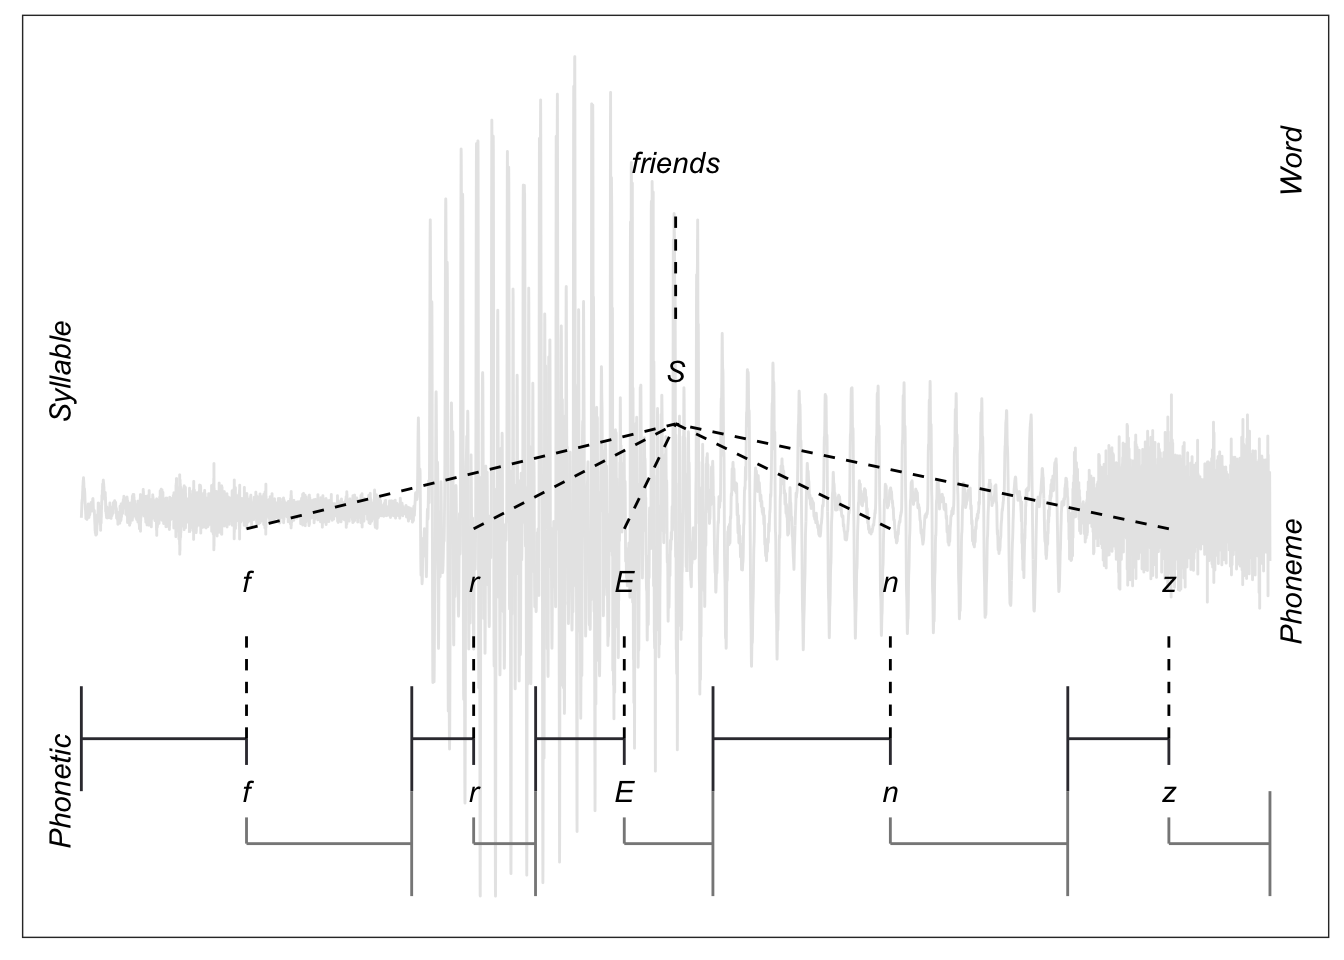
\includegraphics[width=0.75\linewidth]{overview_files/figure-latex/overview-hybridAnnot-1} 

}

\caption{Example of a hybrid annotation combining time-based (*Phonetic* level) and hierarchical (*Phoneme*, *Syllable*, *Text* levels including the inter-level links) annotations.}\label{fig:overview-hybridAnnot}
\end{figure}

Further, to our knowledge, the EMU-SDMS is the first system that makes use of a web application as its primary GUI for annotating speech. This unique approach enables the GUI component to be used in multiple ways. It can be used as a stand-alone annotation tool, connected to a loaded \texttt{emuDB} via \texttt{emuR}'s \texttt{serve()} function and used to communicate to other servers. This enables it to be used as a collaborative annotation tool. An in-depth explanation of how this component can be used in these three scenarios is given in Chapter \ref{chap:emu-webApp}.

As demonstrated in the default workflow of Section \ref{sec:overview-sysArch}, an additional unique feature provided by EMU-SDMS is the ability to use the result of a query to extract derived (e.g., formants and RMS values) and complementary signals (e.g., electromagnetic articulography (EMA) data) that match the segments of a query. This, for example, aids the user in answering questions related to derived speech signals such as: \emph{Given an annotated speech database, is the vowel height of the vowel @ (measured by its correlate, the first formant frequency) influenced by whether it appears in a content or function word?}. Chapter \ref{chap:tutorial} gives a complete walk-through of how to go about answering this question using the tools provided by the EMU-SDMS.

The features provided by the EMU-SDMS make it an all-in-one speech database management solution that is centered around R. It enriches the R platform by providing specialized speech signal processing, speech database management, data extraction and speech annotation capabilities. By achieving this without relying on any external software sources except the web browser, the EMU-SDMS significantly reduces the number of tools the speech and spoken language researcher has to deal with and helps to simplify answering research questions. As the only prerequisite for using the EMU-SDMS is a basic familiarity with the R platform, if the above features would improve your workflow, the EMU-SDMS is indeed for you.

\hypertarget{chap:tutorial}{%
\chapter[A tutorial on how to use the EMU-SDMS ]{\texorpdfstring{A tutorial on how to use the EMU-SDMS \footnote{Some examples of this chapter are adapted versions of examples of the \texttt{emuR\_intro} vignette.}}{A tutorial on how to use the EMU-SDMS }}\label{chap:tutorial}}

\begin{center}\includegraphics[width=0.65\linewidth]{pics/emuSdmsBirdsEye} \end{center}

Using the tools provided by the EMU-SDMS, this tutorial chapter gives a practical step-by-step guide to answering the question: \emph{Given an annotated speech database, is the vowel height of the vowel @ (measured by its correlate, the first formant frequency) influenced by whether it appears in a content or function word?} The tutorial only skims over many of the concepts and functions provided by the EMU-SDMS. In-depth explanations of the various functionalities are given in later chapters of this documentation.

As the EMU-SDMS is not concerned with the raw data acquisition, other tools such as SpeechRecorder by \citet{draxler:2004a} are first used to record speech. However, once audio speech recordings are available, the system provides multiple conversion routines for converting existing collections of files to the new \texttt{emuDB} format described in Chapter \ref{chap:emuDB} and importing them into the new EMU system. The current import routines provided by the \texttt{emuR} package are:

\begin{itemize}
\tightlist
\item
  \texttt{convert\_TextGridCollection()} - Convert TextGrid collections (\texttt{.wav} and \texttt{.TextGrid} files) to the \texttt{emuDB} format,
\item
  \texttt{convert\_BPFCollection()} - Convert Bas Partitur Format (BPF) collections (\texttt{.wav} and \texttt{.par} files) to the \texttt{emuDB} format,
\item
  \texttt{convert\_txtCollection()} - Convert plain text file collections format (\texttt{.wav} and \texttt{.txt} files) to the \texttt{emuDB} format,
\item
  \texttt{convert\_legacyEmuDB()} - Convert the legacy EMU database format to the \texttt{emuDB} format and
\item
  \texttt{create\_emuDB()} followed by \texttt{add\_link/levelDefinition} and \texttt{import\_mediaFiles()} - Creating \texttt{emuDB}s from scratch with only audio files present.
\end{itemize}

The \texttt{emuR} package comes with a set of example files and small databases that are used throughout the \texttt{emuR} documentation, including the functions help pages. These can be accessed by typing \texttt{help(function\_name)} or the short form \texttt{?function\_name}. R code snippet below illustrates how to create this demo data in a user-specified directory. Throughout the examples of this documentation the directory that is provided by the base R function \texttt{tempdir()} will be used, as this is available on every platform supported by R (see \texttt{?tempdir} for further details). As can be inferred from the \texttt{list.dirs()} output in the below code, the \texttt{emuR\_demoData} directory contains a separate directory containing example data for each of the import routines. Additionally, it contains a directory containing an \texttt{emuDB} called \emph{ae} (the directories name is \texttt{ae\_emuDB}, where \texttt{\_emuDB} is the default suffix given to directories containing a \texttt{emuDB}; see Chapter \ref{chap:emuDB}).

\begin{Shaded}
\begin{Highlighting}[]
\CommentTok{# load the package}
\KeywordTok{library}\NormalTok{(emuR)}

\CommentTok{# create demo data in directory provided by the tempdir() function}
\CommentTok{# (of course other directory paths may be chosen)}
\KeywordTok{create_emuRdemoData}\NormalTok{(}\DataTypeTok{dir =} \KeywordTok{tempdir}\NormalTok{())}

\CommentTok{# create path to demo data directory, which is}
\CommentTok{# called "emuR_demoData"}
\NormalTok{demo_data_dir =}\StringTok{ }\KeywordTok{file.path}\NormalTok{(}\KeywordTok{tempdir}\NormalTok{(), }\StringTok{"emuR_demoData"}\NormalTok{)}

\CommentTok{# show demo data directories}
\KeywordTok{list.dirs}\NormalTok{(demo_data_dir, }\DataTypeTok{recursive =}\NormalTok{ F, }\DataTypeTok{full.names =}\NormalTok{ F)}
\end{Highlighting}
\end{Shaded}

\begin{verbatim}
## [1] "ae_emuDB"            "BPF_collection"      "legacy_ae"          
## [4] "TextGrid_collection" "txt_collection"
\end{verbatim}

This tutorial will start by converting a TextGrid collection containing seven annotated single-sentence utterances of a single male speaker to the \texttt{emuDB} format\footnote{The other input routines are covered in the Section @ref(sec:emuRpackageDetails\_importRoutines).}. In the EMU-SDMS, a file collection such as a TextGrid collection refers to a set of file pairs where two types of files with different file extentions are present (e.g., \texttt{.ext1} and \texttt{.ext2}). It is vital that file pairs have the same basenames (e.g., \texttt{A.ext1} and \texttt{A.ext2} where \texttt{A} represents the basename) in order for the conversion functions to be able to pair up files that belong together. As other speech software tools also encourage such file pairs (e.g., \citet{kisler:2015a}) this is a common collection format in the speech sciences. The R code snippet below shows such a file collection that is part of \texttt{emuR}'s demo data. Figure \ref{fig:msajc003-praatTG} shows the content of an annotation as displayed by Praat's \texttt{"Draw\ visible\ sound\ and\ Textgrid..."} procedure.

\begin{Shaded}
\begin{Highlighting}[]
\CommentTok{# create path to TextGrid collection}
\NormalTok{tg_col_dir =}\StringTok{ }\KeywordTok{file.path}\NormalTok{(demo_data_dir, }\StringTok{"TextGrid_collection"}\NormalTok{)}

\CommentTok{# show content of TextGrid_collection directory}
\KeywordTok{list.files}\NormalTok{(tg_col_dir)}
\end{Highlighting}
\end{Shaded}

\begin{verbatim}
##  [1] "msajc003.TextGrid" "msajc003.wav"      "msajc010.TextGrid"
##  [4] "msajc010.wav"      "msajc012.TextGrid" "msajc012.wav"     
##  [7] "msajc015.TextGrid" "msajc015.wav"      "msajc022.TextGrid"
## [10] "msajc022.wav"      "msajc023.TextGrid" "msajc023.wav"     
## [13] "msajc057.TextGrid" "msajc057.wav"
\end{verbatim}

\textbackslash{}begin\{figure\}

\{\centering \includegraphics[width=0.85\linewidth]{pics/msajc003_praat}

\}

\textbackslash{}caption\{TextGrid annotation of the \texttt{emuR\_demoData/TextGrid\_collection/msajc003.wav} / \texttt{.TextGrid} file pair containing the tiers (from top to bottom): \emph{Utterance}, \emph{Intonational}, \emph{Intermediate}, \emph{Word}, \emph{Accent}, \emph{Text}, \emph{Syllable}, \emph{Phoneme}, \emph{Phonetic}, \emph{Tone}, \emph{Foot}.\}\label{fig:msajc003-praatTG}
\textbackslash{}end\{figure\}

\hypertarget{converting-the-textgrid-collection}{%
\section{Converting the TextGrid collection}\label{converting-the-textgrid-collection}}

The \texttt{convert\_TextGridCollection()} function converts a TextGrid collection to the \texttt{emuDB} format. A precondition that all \texttt{.TextGrid} files have to fulfill is that they must all contain the same tiers. If this is not the case, yet there is an equal tier subset that is contained in all the TextGrid files, this equal subset may be chosen. For example, if all \texttt{.TextGrid} files contain only the tier \texttt{Phonetic:\ IntervalTier} the conversion will work. However, if a single \texttt{.TextGrid} of the collection has the additional tier \texttt{Tone:\ TextTier} the conversion will fail. In this case the conversion could be made to work by specifying the equal subset (e.g., \texttt{equalSubset\ =\ c("Phonetic")}) and passing it on to the \texttt{tierNames} function argument \texttt{convert\_TextGridCollection(...,\ tierNames\ =\ equalSubset,\ ...)}. As can be seen in Figure \ref{fig:msajc003-praatTG}, the TextGrid files provided by the demo data contain eleven tiers. To reduce the complexity of the annotations for this tutorial we will only convert the tiers \emph{Word} (content: \emph{C} vs.~function: \emph{F} word annotations), \emph{Syllable} (strong: \emph{S} vs.~weak: \emph{W} syllable annotations), \emph{Phoneme} (phoneme level annotations) and \emph{Phonetic} (phonetic annotations using Speech Assessment Methods Phonetic Alphabet (SAMPA) symbols - \citet{wells:1997aa}) using the \texttt{tierNames} parameter. This conversion can be seen in the R code snippet below.

\begin{Shaded}
\begin{Highlighting}[]
\CommentTok{# convert TextGrid collection to the emuDB format}
\KeywordTok{convert_TextGridCollection}\NormalTok{(}\DataTypeTok{dir =}\NormalTok{ tg_col_dir,}
                           \DataTypeTok{dbName =} \StringTok{"my-first"}\NormalTok{,}
                           \DataTypeTok{targetDir =} \KeywordTok{tempdir}\NormalTok{(),}
                           \DataTypeTok{tierNames =} \KeywordTok{c}\NormalTok{(}\StringTok{"Word"}\NormalTok{, }\StringTok{"Syllable"}\NormalTok{,}
                                         \StringTok{"Phoneme"}\NormalTok{, }\StringTok{"Phonetic"}\NormalTok{))}
\end{Highlighting}
\end{Shaded}

The above call to \texttt{convert\_TextGridCollection()} creates a new \texttt{emuDB} directory in the \texttt{tempdir()} directory called \texttt{my-first\_emuDB}. This \texttt{emuDB} contains annotation files that contain the same \emph{Word}, \emph{Syllable}, \emph{Phoneme} and \emph{Phonetic} segment tiers as the original \texttt{.TextGrid} files as well as copies of the original (\texttt{.wav}) audio files. For further details about the structure of an \texttt{emuDB}, see Chapter \ref{chap:emuDB} of this document.

\hypertarget{loading-and-inspecting-the-database}{%
\section{Loading and inspecting the database}\label{loading-and-inspecting-the-database}}

As mentioned in Section \ref{sec:overview-sysArch}, the first step when working with an \texttt{emuDB} is to load it into the current R session. The R code snippet below shows how to load the converted TextGrid collection into R using the \texttt{load\_emuDB()} function.

\begin{Shaded}
\begin{Highlighting}[]
\CommentTok{# get path to emuDB called "my-first"}
\CommentTok{# that was created by convert_TextGridCollection()}
\NormalTok{path2directory =}\StringTok{ }\KeywordTok{file.path}\NormalTok{(}\KeywordTok{tempdir}\NormalTok{(), }\StringTok{"my-first_emuDB"}\NormalTok{)}

\CommentTok{# load emuDB into current R session}
\CommentTok{# (verbose = F is only set to avoid additional output in manual)}
\NormalTok{db_handle =}\StringTok{ }\KeywordTok{load_emuDB}\NormalTok{(path2directory, }
                       \DataTypeTok{verbose =} \OtherTok{FALSE}\NormalTok{)}
\end{Highlighting}
\end{Shaded}

\hypertarget{overview}{%
\subsection{Overview}\label{overview}}

Now the \emph{my-first} \texttt{emuDB} is loaded into R, an overview of the current status and configuration of the database can be displayed using the \texttt{summary()} function as is shown by the below R code snippet.

\begin{Shaded}
\begin{Highlighting}[]
\CommentTok{# show summary}
\KeywordTok{summary}\NormalTok{(db_handle)}
\end{Highlighting}
\end{Shaded}

\begin{verbatim}
## Name:     my-first 
## UUID:     f0dd8964-7c7c-4cea-a561-624ba406dce5 
## Directory:    /private/var/folders/yk/8z9tn7kx6hbcg_9n4c1sld980000gn/T/RtmpuMOuRJ/my-first_emuDB 
## Session count: 1 
## Bundle count: 7 
## Annotation item count:  664 
## Label count:  664 
## Link count:  0 
## 
## Database configuration:
## 
## SSFF track definitions:
## NULL
## 
## Level definitions:
##       name    type nrOfAttrDefs attrDefNames
## 1     Word SEGMENT            1        Word;
## 2 Syllable SEGMENT            1    Syllable;
## 3  Phoneme SEGMENT            1     Phoneme;
## 4 Phonetic SEGMENT            1    Phonetic;
## 
## Link definitions:
## NULL
\end{verbatim}

The extensive output of \texttt{summary()} is split into a top and bottom half, where the top half focuses on general information about the database (name, directory, annotation item count, etc.) and the bottom half displays information about the various SSFF track, level and link definitions of the \texttt{emuDB}. The summary information about the level definitions shows, for instance, that the \emph{my-first} database has a \emph{Word} level of type \texttt{SEGMENT} and therefore contains annotation items that have a start time and a segment duration. It is worth noting that information about the SSFF track, level and link definitions corresponds to the output of the \texttt{list\_ssffTrackDefinitions()}, \texttt{list\_levelDefinitions()} and \texttt{list\_linkDefinitions()} functions.

\hypertarget{database-annotation-and-visual-inspection}{%
\subsection{Database annotation and visual inspection}\label{database-annotation-and-visual-inspection}}

The EMU-SDMS has a unique approach to annotating and visually inspecting databases, as it utilizes a web application called the \texttt{EMU-webApp} to act as its GUI. To be able to communicate with the web application the \texttt{emuR} package provides the \texttt{serve()} function which is used in the R code snippet below.

\begin{Shaded}
\begin{Highlighting}[]
\CommentTok{# serve my-first emuDB to the EMU-webApp}
\KeywordTok{serve}\NormalTok{(db_handle)}
\end{Highlighting}
\end{Shaded}

Executing this command will either automatically open up the system's default browser or, if using RStudio, download the current EMU-webApp and display it in RStudio's viewer pane and additionally display the following message in the R console:

\begin{verbatim}
## Navigate your browser to the EMU-webApp URL: 
##  https://ips-lmu.github.io/EMU-webApp/ (should happen autom...
## Server connection URL:
##  ws://localhost:17890
## To stop the server either press the 'clear' button in the EMU-webApp, 
##  close/reload the webApp in your browser,
## or call the httpuv::stopAllServers() function
\end{verbatim}

The \texttt{EMU-webApp}, which is now connected to the database via the \texttt{serve()} function, can be used to visually inspect and annotate the \texttt{emuDB}. Figure \ref{fig:tutorial-emuWebAppMyFirst} displays a screenshot of what the \texttt{EMU-webApp} looks like after automatically connecting to the server. As the \texttt{EMU-webApp} is a very feature-rich software annotation tool, this documentation has a whole chapter (see Chapter \ref{chap:emu-webApp}) on how to use it, what it is capable of and how to configure it. To close the connection and free up the blocked R console, simply click the \texttt{clear} button in the top menu bar of the \texttt{EMU-webApp}.

\begin{figure}

{\centering \includegraphics[width=1\linewidth]{pics/tutorialEmuWebAppMyFirst} 

}

\caption{Screenshot of `EMU-webApp` displaying `msajc003` bundle of *my-first* `emuDB`.}\label{fig:tutorial-emuWebAppMyFirst}
\end{figure}

\hypertarget{querying-and-autobuilding-the-annotation-structure}{%
\section{Querying and autobuilding the annotation structure}\label{querying-and-autobuilding-the-annotation-structure}}

An integral step in the default workflow of the EMU-SDMS is querying the annotations of a database. The \texttt{emuR} package implements a \texttt{query()} function to accomplish this task. This function evaluates an EMU Query Language (EQL) expression and extracts the annotation items from the database that match a query expression. As chapter \ref{chap:querysys} gives a detailed description of the query mechanics provided by \texttt{emuR}, this tutorial will only use a very small, hopefully easy to understand subset of the EQL.

The output of the \texttt{summary()} command in the R code snippet below and the screenshot in Figure \ref{fig:tutorial-emuWebAppMyFirst} show that the \emph{my-first} \texttt{emuDB} contains four levels of annotations. The R code snippet below shows four separate queries that query various segments on each of the available levels. The query expressions all use the matching operator \texttt{==} which returns annotation items whose labels match those specified to the right of the operator and that belong to the level specified to the left of the operator (i.e., \texttt{LEVEL\ ==\ LABEL}; see Chapter \ref{chap:querysys} for a detailed description).

\begin{Shaded}
\begin{Highlighting}[]
\CommentTok{# query all segments containing the label}
\CommentTok{# "C" (== content word) of the "Word" level}
\NormalTok{sl_text =}\StringTok{ }\KeywordTok{query}\NormalTok{(}\DataTypeTok{emuDBhandle =}\NormalTok{ db_handle,}
                \DataTypeTok{query =} \StringTok{"Word == C"}\NormalTok{)}

\CommentTok{# query all segments containing the label}
\CommentTok{# "S" (== strong syllable) of the "Syllable" level}
\NormalTok{sl_syl =}\StringTok{ }\KeywordTok{query}\NormalTok{(}\DataTypeTok{emuDBhandle =}\NormalTok{ db_handle,}
               \DataTypeTok{query =} \StringTok{"Syllable == S"}\NormalTok{)}

\CommentTok{# query all segments containing the label}
\CommentTok{# "f" on the "Phoneme" level}
\NormalTok{sl_phoneme =}\StringTok{ }\KeywordTok{query}\NormalTok{(db_handle,}
                   \DataTypeTok{query =} \StringTok{"Phoneme == f"}\NormalTok{)}

\CommentTok{# query all segments containing the label}
\CommentTok{# "n" of the "Phonetic" level}
\NormalTok{sl_phonetic =}\StringTok{ }\KeywordTok{query}\NormalTok{(db_handle,}
                    \DataTypeTok{query =} \StringTok{"Phonetic == n"}\NormalTok{)}

\CommentTok{# show class vector of query result}
\KeywordTok{class}\NormalTok{(sl_phonetic)}
\end{Highlighting}
\end{Shaded}

\begin{verbatim}
## [1] "tbl_df"     "tbl"        "data.frame"
\end{verbatim}

\begin{Shaded}
\begin{Highlighting}[]
\CommentTok{# show first few entries of sl_phonetic}
\NormalTok{sl_phonetic}
\end{Highlighting}
\end{Shaded}

\begin{verbatim}
## # A tibble: 12 x 16
##    labels start   end db_uuid session bundle start_item_id end_item_id level
##    <chr>  <dbl> <dbl> <chr>   <chr>   <chr>          <int>       <int> <chr>
##  1 n      1032. 1196. f0dd89~ 0000    msajc~            98          98 Phon~
##  2 n      1741. 1791. f0dd89~ 0000    msajc~           108         108 Phon~
##  3 n      1515. 1554. f0dd89~ 0000    msajc~           113         113 Phon~
##  4 n      2431. 2528. f0dd89~ 0000    msajc~           127         127 Phon~
##  5 n       895. 1023. f0dd89~ 0000    msajc~            98          98 Phon~
##  6 n      2402. 2475. f0dd89~ 0000    msajc~           122         122 Phon~
##  7 n      2227. 2271. f0dd89~ 0000    msajc~           132         132 Phon~
##  8 n      3046. 3068. f0dd89~ 0000    msajc~           145         145 Phon~
##  9 n      1435. 1495. f0dd89~ 0000    msajc~            91          91 Phon~
## 10 n      1775. 1834. f0dd89~ 0000    msajc~            96          96 Phon~
## 11 n       509.  544. f0dd89~ 0000    msajc~            97          97 Phon~
## 12 n      2448. 2480. f0dd89~ 0000    msajc~           130         130 Phon~
## # ... with 7 more variables: attribute <chr>, start_item_seq_idx <int>,
## #   end_item_seq_idx <int>, type <chr>, sample_start <int>, sample_end <int>,
## #   sample_rate <int>
\end{verbatim}

As demonstrated in the above R code, the result of a query is a \texttt{tbl\_df} object (i.e.~a \href{https://tibble.tidyverse.org/index.html}{tibble object}), which is a super-class of the common \texttt{data.frame}. For historical reasons the result of a query is often referred to as a segment list, or ``seglist''. A segment list carries information about the extracted annotation items such as the extracted labels, the start and end times of the segments, the sessions and bundles the items are from and the levels they belong to. An in-depth description of the information contained in a segment list is given in Section \ref{sec:query-emuRsegs}.

\hypertarget{autobuilding}{%
\section{Autobuilding}\label{autobuilding}}

The simple queries illustrated above query segments from a single level that match a certain label. However, the EMU-SDMS offers a mechanism for performing inter-level queries such as: \emph{Query all Phonetic items that contain the label ``n'' and are part of a content word}. For such queries to be possible, the EMU-SDMS offers very sophisticated annotation structure modeling capabilities, which are described in Chapter \ref{chap:annot-struct-mod}. For the sake of this tutorial we will focus on converting the flat segment level annotation structure displayed in Figure \ref{fig:tutorial-emuWebAppMyFirst} to a hierarchical form as displayed in Figure \ref{fig:tutorial-violentlyHier}, where only the \emph{Phonetic} level carries time information and the annotation items on the other levels are explicitly linked to each other to form a hierarchical annotation structure.

\begin{figure}

{\centering 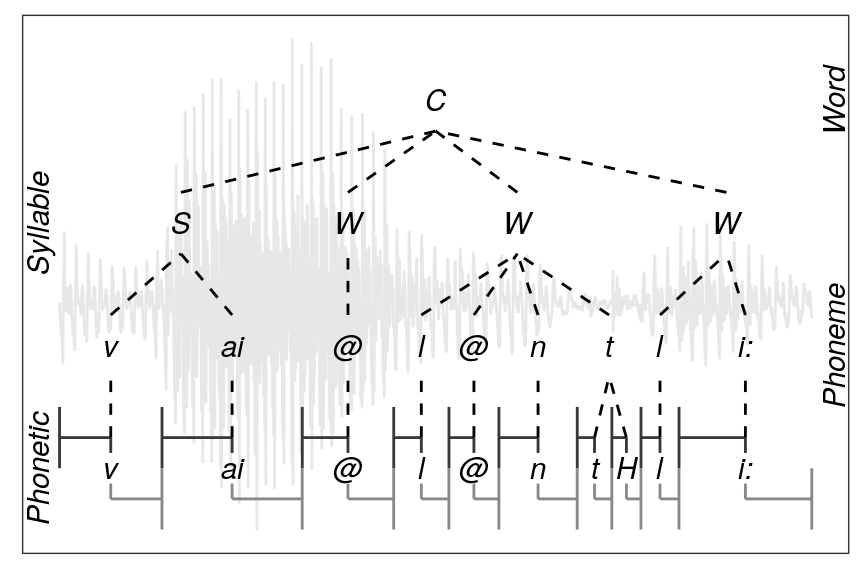
\includegraphics{tutorial_files/figure-latex/tutorial-violentlyHier-1} 

}

\caption{Example of a hierarchical annotation of the content (==*C*) word *violently* belonging to the *msajc012* bundle of the *my-first* demo `emuDB`.}\label{fig:tutorial-violentlyHier}
\end{figure}

As it is a very laborious task to manually link annotation items together using the \texttt{EMU-webApp} and the hierarchical information is already implicitly contained in the time information of the segments and events of each level, we will now use a function provided by the \texttt{emuR} package to build these hierarchical structures using this information called \texttt{autobuild\_linkFromTimes()}. The above R code snippet shows the calls to this function which autobuild the hierarchical annotations in the \emph{my-first} database. As a general rule for autobuilding hierarchical annotation structures, a good strategy is to start the autobuilding process beginning with coarser grained annotation levels (i.e., the \emph{Word}/\emph{Syllable} level pair in our example) and work down to finer grained annotations (i.e., the \emph{Syllable}/\emph{Phoneme} and \emph{Phoneme}/\emph{Phonetic} level pairs in our example). To build hierachical annotation structures we need link definitions, which together with the level definitions define the annotation structure for the entire database (see Chapter \ref{chap:annot-struct-mod} for further details). The \texttt{autobuild\_linkFromTimes()} calls in the below R code snippet use the \texttt{newLinkDefType} parameter, which if defined automatically adds a link definition to the database.

\begin{Shaded}
\begin{Highlighting}[]
\CommentTok{# invoke autobuild function}
\CommentTok{# for "Word" and "Syllable" levels}
\KeywordTok{autobuild_linkFromTimes}\NormalTok{(db_handle,}
                        \DataTypeTok{superlevelName =} \StringTok{"Word"}\NormalTok{,}
                        \DataTypeTok{sublevelName =} \StringTok{"Syllable"}\NormalTok{,}
                        \DataTypeTok{convertSuperlevel =} \OtherTok{TRUE}\NormalTok{,}
                        \DataTypeTok{newLinkDefType =} \StringTok{"ONE_TO_MANY"}\NormalTok{)}

\CommentTok{# invoke autobuild function}
\CommentTok{# for "Syllable" and "Phoneme" levels}
\KeywordTok{autobuild_linkFromTimes}\NormalTok{(db_handle,}
                        \DataTypeTok{superlevelName =} \StringTok{"Syllable"}\NormalTok{,}
                        \DataTypeTok{sublevelName =} \StringTok{"Phoneme"}\NormalTok{,}
                        \DataTypeTok{convertSuperlevel =} \OtherTok{TRUE}\NormalTok{,}
                        \DataTypeTok{newLinkDefType =} \StringTok{"ONE_TO_MANY"}\NormalTok{)}

\CommentTok{# invoke autobuild function}
\CommentTok{# for "Phoneme" and "Phonetic" levels}
\KeywordTok{autobuild_linkFromTimes}\NormalTok{(db_handle,}
                        \DataTypeTok{superlevelName =} \StringTok{"Phoneme"}\NormalTok{,}
                        \DataTypeTok{sublevelName =} \StringTok{"Phonetic"}\NormalTok{,}
                        \DataTypeTok{convertSuperlevel =} \OtherTok{TRUE}\NormalTok{,}
                        \DataTypeTok{newLinkDefType =} \StringTok{"MANY_TO_MANY"}\NormalTok{)}
\end{Highlighting}
\end{Shaded}

\begin{figure}

{\centering \includegraphics[width=0.5\linewidth]{pics/tut_simpleAnnotStruct} 

}

\caption{Schematic annotation structure of the `emuDB` after calling the autobuild function in R code snippet above.}\label{fig:tutorial-simpleAnnotStruct}
\end{figure}

As the \texttt{autobuild\_linkFromTimes()} function automatically creates backup levels to avoid the accidental loss of boundary or event time information, the R code snippet below shows how these backup levels can be removed to clean up the database. However, using the \texttt{remove\_levelDefinition()} function with its \texttt{force} parameter set to \texttt{TRUE} is a very invasive action. Usually this would not be recommended, but for this tutorial we are keeping everything as clean as possible.

\begin{Shaded}
\begin{Highlighting}[]
\CommentTok{# list level definitions}
\CommentTok{# as this reveals the "-autobuildBackup" levels}
\CommentTok{# added by the autobuild_linkFromTimes() calls}
\KeywordTok{list_levelDefinitions}\NormalTok{(db_handle)}
\end{Highlighting}
\end{Shaded}

\begin{verbatim}
##                       name    type nrOfAttrDefs              attrDefNames
## 1                     Word    ITEM            1                     Word;
## 2                 Syllable    ITEM            1                 Syllable;
## 3                  Phoneme    ITEM            1                  Phoneme;
## 4                 Phonetic SEGMENT            1                 Phonetic;
## 5     Word-autobuildBackup SEGMENT            1     Word-autobuildBackup;
## 6 Syllable-autobuildBackup SEGMENT            1 Syllable-autobuildBackup;
## 7  Phoneme-autobuildBackup SEGMENT            1  Phoneme-autobuildBackup;
\end{verbatim}

\begin{Shaded}
\begin{Highlighting}[]
\CommentTok{# remove the levels containing the "-autobuildBackup"}
\CommentTok{# suffix}
\CommentTok{# (verbose = F is only set to avoid additional output in manual)}
\KeywordTok{remove_levelDefinition}\NormalTok{(db_handle,}
                       \DataTypeTok{name =} \StringTok{"Word-autobuildBackup"}\NormalTok{,}
                       \DataTypeTok{force =} \OtherTok{TRUE}\NormalTok{,}
                       \DataTypeTok{verbose =} \OtherTok{FALSE}\NormalTok{)}
\CommentTok{# (verbose = F is only set to avoid additional output in manual)}
\KeywordTok{remove_levelDefinition}\NormalTok{(db_handle,}
                       \DataTypeTok{name =} \StringTok{"Syllable-autobuildBackup"}\NormalTok{,}
                       \DataTypeTok{force =} \OtherTok{TRUE}\NormalTok{,}
                       \DataTypeTok{verbose =} \OtherTok{FALSE}\NormalTok{)}
\CommentTok{# (verbose = F is only set to avoid additional output in manual)}
\KeywordTok{remove_levelDefinition}\NormalTok{(db_handle,}
                       \DataTypeTok{name =} \StringTok{"Phoneme-autobuildBackup"}\NormalTok{,}
                       \DataTypeTok{force =} \OtherTok{TRUE}\NormalTok{,}
                       \DataTypeTok{verbose =} \OtherTok{FALSE}\NormalTok{)}

\CommentTok{# list level definitions}
\KeywordTok{list_levelDefinitions}\NormalTok{(db_handle)}
\end{Highlighting}
\end{Shaded}

\begin{verbatim}
##       name    type nrOfAttrDefs attrDefNames
## 1     Word    ITEM            1        Word;
## 2 Syllable    ITEM            1    Syllable;
## 3  Phoneme    ITEM            1     Phoneme;
## 4 Phonetic SEGMENT            1    Phonetic;
\end{verbatim}

\begin{Shaded}
\begin{Highlighting}[]
\CommentTok{# list level definitions}
\CommentTok{# which were added by the autobuild functions}
\KeywordTok{list_linkDefinitions}\NormalTok{(db_handle)}
\end{Highlighting}
\end{Shaded}

\begin{verbatim}
##           type superlevelName sublevelName
## 1  ONE_TO_MANY           Word     Syllable
## 2  ONE_TO_MANY       Syllable      Phoneme
## 3 MANY_TO_MANY        Phoneme     Phonetic
\end{verbatim}

As can be seen by the output of \texttt{list\_levelDefinitions()} and \texttt{list\_linkDefinitions()} in the above R code, the annotation structure of the \emph{my-first} \texttt{emuDB} now matches that displayed in Figure \ref{fig:tutorial-simpleAnnotStruct}. Using the \texttt{serve()} function to open the \texttt{emuDB} in the \texttt{EMU-webApp} followed by clicking on the \texttt{show\ hierarchy} button in the top menu (and rotating the hierarchy by 90 degrees by clicking the \texttt{rotate\ by\ 90\ degrees} button) will result in a view similar to the screenshot of Figure \ref{fig:tutorial-EMU-webAppScreenshotTutorialPostAutobHier}.

\begin{figure}

{\centering \includegraphics[width=1\linewidth]{pics/EMU-webAppScreenshotTutorialPostAutobHier} 

}

\caption{Screenshot of `EMU-webApp` displaying the autobuilt hierarchy of the *my-first* `emuDB`.}\label{fig:tutorial-EMU-webAppScreenshotTutorialPostAutobHier}
\end{figure}

\hypertarget{querying-the-hierarchical-annotations}{%
\subsection{Querying the hierarchical annotations}\label{querying-the-hierarchical-annotations}}

Having this hierarchical annotation structure now allows us to formulate a query that helps answer the originally stated question: \emph{Given an annotated speech database, is the vowel height of the vowel @ (measured by its correlate, the first formant frequency) influenced by whether it appears in a content or function word?}. The R code snippet below shows how all the \emph{@} vowels in the \emph{my-first} database are queried.

\begin{Shaded}
\begin{Highlighting}[]
\CommentTok{# query annotation items containing}
\CommentTok{# the labels @ on the Phonetic level}
\NormalTok{sl_vowels =}\StringTok{ }\KeywordTok{query}\NormalTok{(db_handle, }\StringTok{"Phonetic == @"}\NormalTok{)}

\CommentTok{# show sl_vowels}
\NormalTok{sl_vowels}
\end{Highlighting}
\end{Shaded}

\begin{verbatim}
## # A tibble: 28 x 16
##    labels start   end db_uuid session bundle start_item_id end_item_id level
##    <chr>  <dbl> <dbl> <chr>   <chr>   <chr>          <int>       <int> <chr>
##  1 @      1506. 1548. f0dd89~ 0000    msajc~           103         103 Phon~
##  2 @      1715. 1741. f0dd89~ 0000    msajc~           107         107 Phon~
##  3 @      1967. 2034. f0dd89~ 0000    msajc~           112         112 Phon~
##  4 @      2303. 2362. f0dd89~ 0000    msajc~           117         117 Phon~
##  5 @      2447. 2506. f0dd89~ 0000    msajc~           119         119 Phon~
##  6 @      1917. 1958. f0dd89~ 0000    msajc~           118         118 Phon~
##  7 @      2022. 2078. f0dd89~ 0000    msajc~           120         120 Phon~
##  8 @      2382. 2431. f0dd89~ 0000    msajc~           126         126 Phon~
##  9 @       330.  380. f0dd89~ 0000    msajc~            91          91 Phon~
## 10 @      1472. 1490. f0dd89~ 0000    msajc~           108         108 Phon~
## # ... with 18 more rows, and 7 more variables: attribute <chr>,
## #   start_item_seq_idx <int>, end_item_seq_idx <int>, type <chr>,
## #   sample_start <int>, sample_end <int>, sample_rate <int>
\end{verbatim}

As the type of word (content vs.~function) for each \emph{@} vowel is also needed, we can use the requery functionality of the EMU-SDMS (see Chapter \ref{chap:querysys}) to retrieve the word type for each \emph{@} vowel. A requery essentially moves through a hierarchical annotation (vertically or horizontally) starting from the segments that are passed into the requery function. The R code below illustrates the usage of the hierarchical requery function, \texttt{requery\_hier()}, to retrieve the appropriate annotation items from the \emph{Word} level.

\begin{Shaded}
\begin{Highlighting}[]
\CommentTok{# hierarchical requery starting from the items in sl_vowels}
\CommentTok{# and moving up to the "Word" level}
\NormalTok{sl_word_type =}\StringTok{ }\KeywordTok{requery_hier}\NormalTok{(db_handle,}
                           \DataTypeTok{seglist =}\NormalTok{ sl_vowels,}
                           \DataTypeTok{level =} \StringTok{"Word"}\NormalTok{,}
                           \DataTypeTok{calcTimes =} \OtherTok{FALSE}\NormalTok{)}

\CommentTok{# show sl_word_type}
\NormalTok{sl_word_type}
\end{Highlighting}
\end{Shaded}

\begin{verbatim}
## # A tibble: 28 x 16
##    labels start   end db_uuid session bundle start_item_id end_item_id level
##    <chr>  <dbl> <dbl> <chr>   <chr>   <chr>          <int>       <int> <chr>
##  1 F         NA    NA f0dd89~ 0000    msajc~            16          16 Word 
##  2 C         NA    NA f0dd89~ 0000    msajc~            17          17 Word 
##  3 C         NA    NA f0dd89~ 0000    msajc~            17          17 Word 
##  4 C         NA    NA f0dd89~ 0000    msajc~            18          18 Word 
##  5 C         NA    NA f0dd89~ 0000    msajc~            18          18 Word 
##  6 C         NA    NA f0dd89~ 0000    msajc~            19          19 Word 
##  7 C         NA    NA f0dd89~ 0000    msajc~            20          20 Word 
##  8 C         NA    NA f0dd89~ 0000    msajc~            20          20 Word 
##  9 F         NA    NA f0dd89~ 0000    msajc~            13          13 Word 
## 10 F         NA    NA f0dd89~ 0000    msajc~            17          17 Word 
## # ... with 18 more rows, and 7 more variables: attribute <chr>,
## #   start_item_seq_idx <int>, end_item_seq_idx <int>, type <chr>,
## #   sample_start <int>, sample_end <int>, sample_rate <int>
\end{verbatim}

\begin{Shaded}
\begin{Highlighting}[]
\CommentTok{# show that sl_vowel and sl_word_type have the}
\CommentTok{# same number of row entries}
\KeywordTok{nrow}\NormalTok{(sl_vowels) }\OperatorTok{==}\StringTok{ }\KeywordTok{nrow}\NormalTok{(sl_word_type)}
\end{Highlighting}
\end{Shaded}

\begin{verbatim}
## [1] TRUE
\end{verbatim}

As can be seen by the \texttt{nrow()} comparison in the above R code, the segment list returned by the \texttt{requery\_hier()} function has the same number of rows as the original \texttt{sl\_vowels} segment list. This is important, as each row of both segment lists line up and allow us to infer which segment belongs to which word type (e.g., vowel \texttt{sl\_vowels{[}5,{]}} belongs to the word type \texttt{sl\_word\_type{[}5,{]}}).

\hypertarget{section:tutorial-sigExtrAndExpl}{%
\section{Signal extraction and exploration}\label{section:tutorial-sigExtrAndExpl}}

Now that the vowel and word type information including the vowel start and end time information has been extracted from the database, this information can be used to extract signal data that matches these segments. Using the \texttt{emuR} function \texttt{get\_trackdata()} we can calculate the formant values in real time using the formant estimation function, \texttt{forest()}, provided by the \texttt{wrassp} package (see Chapter \ref{chap:wrassp} for details). The following R code shows the usage of this function.

\begin{Shaded}
\begin{Highlighting}[]
\CommentTok{# get formant values for the vowel segments}
\CommentTok{# (verbose = F is only set to avoid additional output in manual)}
\NormalTok{td_vowels =}\StringTok{ }\KeywordTok{get_trackdata}\NormalTok{(db_handle,}
                          \DataTypeTok{seglist =}\NormalTok{ sl_vowels,}
                          \DataTypeTok{onTheFlyFunctionName =} \StringTok{"forest"}\NormalTok{,}
                          \DataTypeTok{verbose =}\NormalTok{ F)}

\CommentTok{# show class vector}
\KeywordTok{class}\NormalTok{(td_vowels)}
\end{Highlighting}
\end{Shaded}

\begin{verbatim}
## [1] "tbl_df"     "tbl"        "data.frame"
\end{verbatim}

\begin{Shaded}
\begin{Highlighting}[]
\CommentTok{# show dimensions}
\KeywordTok{dim}\NormalTok{(td_vowels)}
\end{Highlighting}
\end{Shaded}

\begin{verbatim}
## [1] 287  24
\end{verbatim}

\begin{Shaded}
\begin{Highlighting}[]
\CommentTok{# show nr of segments}
\KeywordTok{max}\NormalTok{(td_vowels}\OperatorTok{$}\NormalTok{sl_rowIdx)}
\end{Highlighting}
\end{Shaded}

\begin{verbatim}
## [1] 28
\end{verbatim}

\begin{Shaded}
\begin{Highlighting}[]
\CommentTok{# display all values for fifth segment using dplyr}
\KeywordTok{library}\NormalTok{(dplyr)}
\NormalTok{td_vowels }\OperatorTok\StringTok{ }\KeywordTok{filter}\NormalTok{(sl_rowIdx }\OperatorTok{==}\StringTok{ }\DecValTok{5}\NormalTok{)}
\end{Highlighting}
\end{Shaded}

\begin{verbatim}
## # A tibble: 12 x 24
##    sl_rowIdx labels start   end db_uuid session bundle start_item_id end_item_id
##        <int> <chr>  <dbl> <dbl> <chr>   <chr>   <chr>          <int>       <int>
##  1         5 @      2447. 2506. f0dd89~ 0000    msajc~           119         119
##  2         5 @      2447. 2506. f0dd89~ 0000    msajc~           119         119
##  3         5 @      2447. 2506. f0dd89~ 0000    msajc~           119         119
##  4         5 @      2447. 2506. f0dd89~ 0000    msajc~           119         119
##  5         5 @      2447. 2506. f0dd89~ 0000    msajc~           119         119
##  6         5 @      2447. 2506. f0dd89~ 0000    msajc~           119         119
##  7         5 @      2447. 2506. f0dd89~ 0000    msajc~           119         119
##  8         5 @      2447. 2506. f0dd89~ 0000    msajc~           119         119
##  9         5 @      2447. 2506. f0dd89~ 0000    msajc~           119         119
## 10         5 @      2447. 2506. f0dd89~ 0000    msajc~           119         119
## 11         5 @      2447. 2506. f0dd89~ 0000    msajc~           119         119
## 12         5 @      2447. 2506. f0dd89~ 0000    msajc~           119         119
## # ... with 15 more variables: level <chr>, attribute <chr>,
## #   start_item_seq_idx <int>, end_item_seq_idx <int>, type <chr>,
## #   sample_start <int>, sample_end <int>, sample_rate <int>, times_orig <dbl>,
## #   times_rel <dbl>, times_norm <dbl>, T1 <int>, T2 <int>, T3 <int>, T4 <int>
\end{verbatim}

As can be seen by the call to the \texttt{class()} function, the resulting object is of the type \texttt{tibble} (see \texttt{?tibble::tibble} for more information) and has 28 blocks of data. These blocks correspond to the number of rows contained in the segment lists extracted above (i.e., \texttt{nrow(sl\_vowels)}) and can be matched to the according segment using the \texttt{sl\_rowIdx} column (i.e., \texttt{td\_vowels\ \%\textgreater{}\%\ filter(sl\_rowIdx\ ==\ 5)} are the formant values belonging to \texttt{sl\_vowels{[}5,{]}}). As the columns \texttt{T1}, \texttt{T2}, \texttt{T3}, \texttt{T4} of the printed output of \texttt{td\_vowels\ \%\textgreater{}\%\ filter(sl\_rowIdx\ ==\ 5)} suggest, the \texttt{forest} function estimates four formant values. We will only be concerned with the first (column \texttt{T1}) and second (column \texttt{T2}). The below R code shows two \texttt{ggplot()} function calls which produce the plots displayed in Figures \ref{fig:tutorial-dplot1} and \ref{fig:tutorial-dplot1}. The first \texttt{ggplot()} call plots all 28 first formant trajectories (achieved by setting the \texttt{group} parameter to \texttt{sl\_rowIdx}). To clean up the cluttered first plot, the second \texttt{ggplot()} call uses a segment length normalized version of \texttt{td\_vowels} (see \texttt{?normalize\_length} for futher details) as well as using \texttt{geom\_smooth()} in combination with setting the \texttt{group} parameter to \texttt{labels} to plot only smoothed conditional means of all \emph{@} vowels.

\begin{Shaded}
\begin{Highlighting}[]
\CommentTok{# load package}
\KeywordTok{library}\NormalTok{(ggplot2)}

\KeywordTok{ggplot}\NormalTok{(td_vowels) }\OperatorTok{+}
\StringTok{  }\KeywordTok{aes}\NormalTok{(}\DataTypeTok{x =}\NormalTok{ times_rel, }\DataTypeTok{y =}\NormalTok{ T1, }\DataTypeTok{col =}\NormalTok{ labels, }\DataTypeTok{group =}\NormalTok{ sl_rowIdx) }\OperatorTok{+}
\StringTok{  }\KeywordTok{geom_line}\NormalTok{() }\OperatorTok{+}
\StringTok{  }\KeywordTok{labs}\NormalTok{(}\DataTypeTok{x =} \StringTok{"Duration (ms)"}\NormalTok{, }\DataTypeTok{y =} \StringTok{"F1 (Hz)"}\NormalTok{)}

\CommentTok{# normalize length of segments}
\NormalTok{td_vowels_norm =}\StringTok{ }\KeywordTok{normalize_length}\NormalTok{(td_vowels)}

\KeywordTok{ggplot}\NormalTok{(td_vowels_norm) }\OperatorTok{+}
\StringTok{  }\KeywordTok{aes}\NormalTok{(}\DataTypeTok{x =}\NormalTok{ times_norm, }\DataTypeTok{y =}\NormalTok{ T1, }\DataTypeTok{col =}\NormalTok{ labels, }\DataTypeTok{group =}\NormalTok{ labels) }\OperatorTok{+}
\StringTok{  }\KeywordTok{geom_smooth}\NormalTok{() }\OperatorTok{+}
\StringTok{  }\KeywordTok{labs}\NormalTok{(}\DataTypeTok{x =} \StringTok{"Duration (normalized)"}\NormalTok{, }\DataTypeTok{y =} \StringTok{"F1 (Hz)"}\NormalTok{) }
\end{Highlighting}
\end{Shaded}

\begin{figure}

{\centering 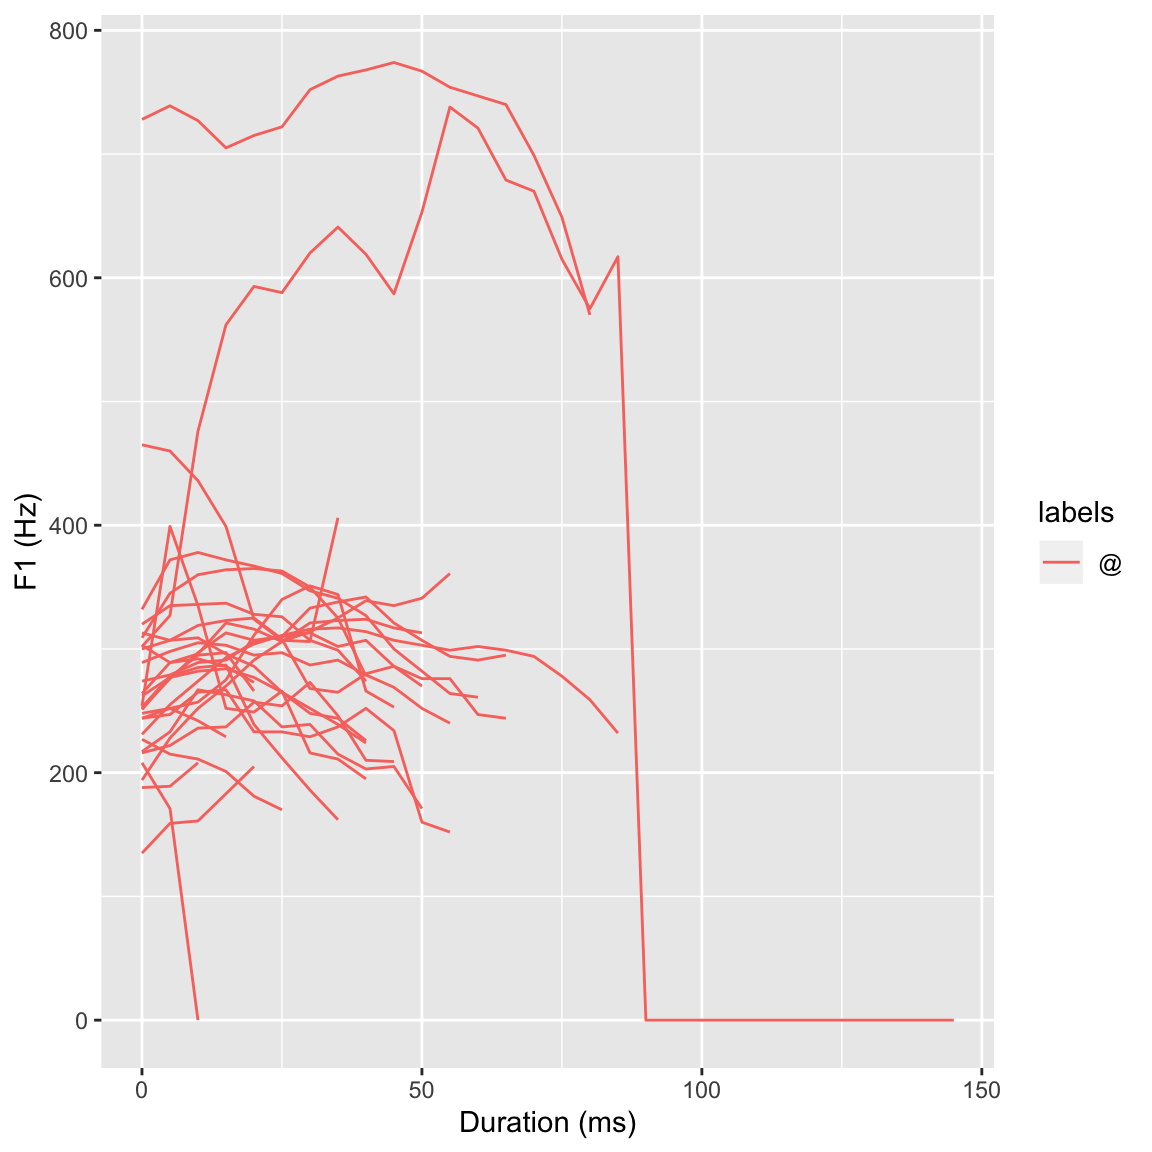
\includegraphics{tutorial_files/figure-latex/tutorial-dplot1-1} 

}

\caption{`ggplot()` plots of all F1 *\@* vowel trajectories.}\label{fig:tutorial-dplot1}
\end{figure}

\begin{figure}

{\centering 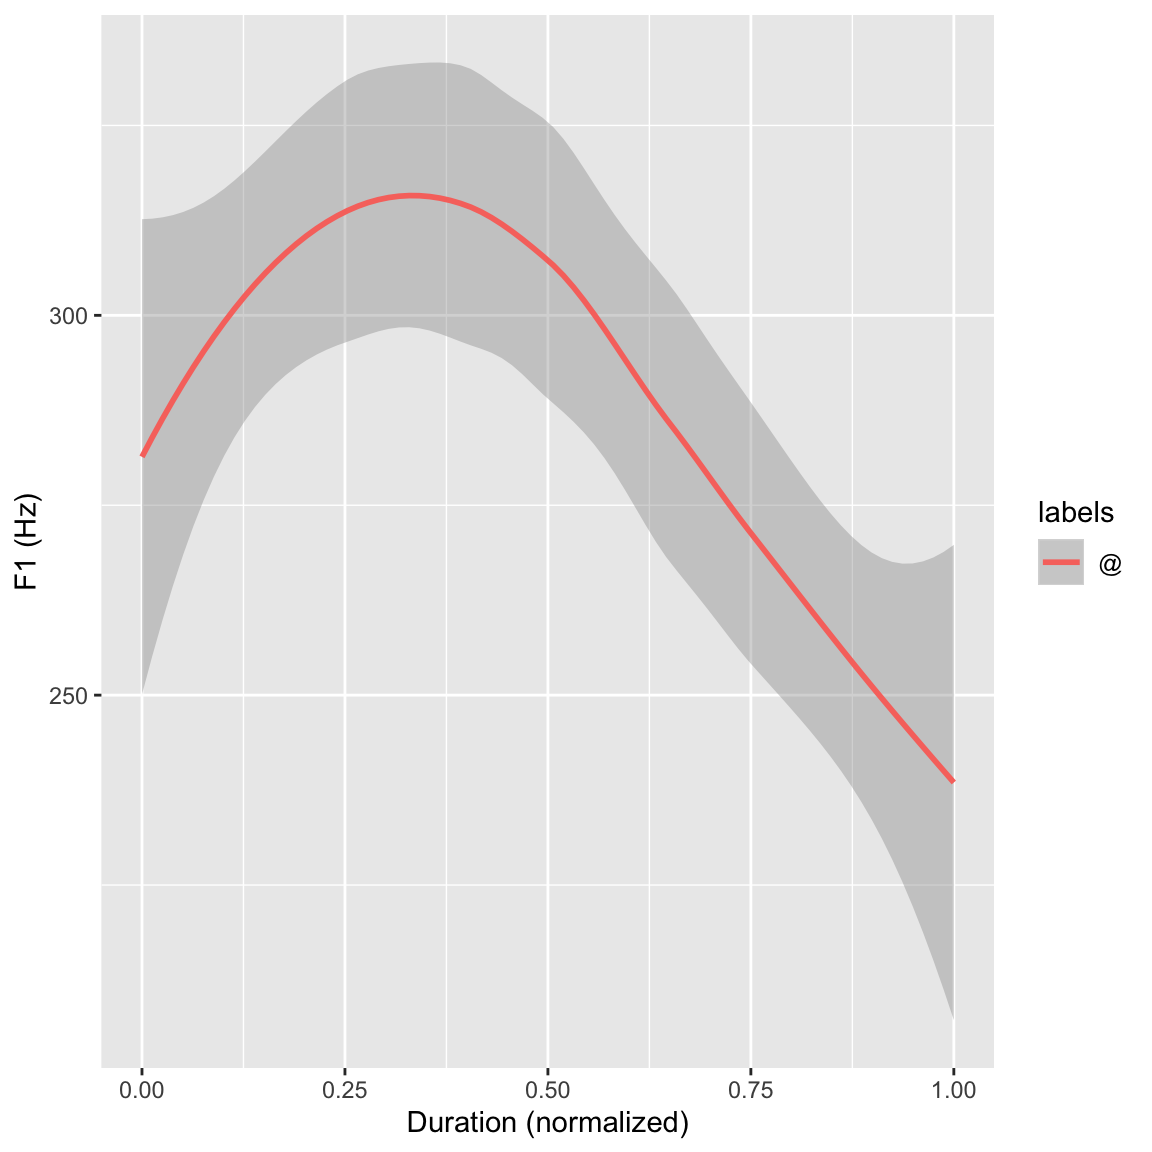
\includegraphics{tutorial_files/figure-latex/tutorial-dplot2-1} 

}

\caption{`ggplot()` plots of the F1 smoothed conditional mean trajectories of all *\@* vowels.}\label{fig:tutorial-dplot2}
\end{figure}

Figures \ref{fig:tutorial-dplot1} and \ref{fig:tutorial-dplot2} give an overview of the first formant trajectories of the \emph{@} vowels. For the purpose of data exploration and to get an idea of where the individual vowel classes lie on the F2 x F1 plane, which indirectly provides information about vowel height and tongue position, the R code below again makes use of the \texttt{ggplot()} function. This produces Figure \ref{fig:tutorial-eplot}. To be able to use the \texttt{stat\_ellipse()} function, the \texttt{td\_vowels\_norm} object first has to be modified, as it contains entire formant trajectories but two dimensional data is needed to be able to display it on the F2 x F1 plain. This can, for example, be achieved by only extracting temporal mid-point formant values for each vowel using the \texttt{get\_trackdata()} function utilizing its \texttt{cut} parameter. The R code snippet below shows an alternative approach using the \texttt{dplyr}'s \texttt{filter()} function to essentially cut the formant trajectories to a specified proportional segment. By only extracting the values that have a normalized time value of 0.5 (\texttt{times\_norm\ ==\ 0.5}) only the formant values that are at the time normalized mid-point (calculated above using the \texttt{normalize\_length()} function) are extracted from the trajectories.

\begin{Shaded}
\begin{Highlighting}[]
\CommentTok{# cut formant trajectories at temporal mid-point}
\NormalTok{td_vowels_midpoint =}\StringTok{ }\NormalTok{td_vowels_norm }\OperatorTok\StringTok{ }
\StringTok{  }\KeywordTok{filter}\NormalTok{(times_norm }\OperatorTok{==}\StringTok{ }\FloatTok{0.5}\NormalTok{)}

\CommentTok{# show dimensions of td_vowels_midpoint}
\KeywordTok{dim}\NormalTok{(td_vowels_midpoint)}

\CommentTok{# calculate centroid }
\NormalTok{td_centroids =}\StringTok{ }\NormalTok{td_vowels_midpoint }\OperatorTok
\StringTok{  }\KeywordTok{group_by}\NormalTok{(labels) }\OperatorTok
\StringTok{  }\KeywordTok{summarise}\NormalTok{(}\DataTypeTok{T1 =} \KeywordTok{mean}\NormalTok{(T1), }\DataTypeTok{T2 =} \KeywordTok{mean}\NormalTok{(T2))}

\CommentTok{# generate plot}
\KeywordTok{ggplot}\NormalTok{(td_vowels_midpoint, }\KeywordTok{aes}\NormalTok{(}\DataTypeTok{x =}\NormalTok{ T2, }\DataTypeTok{y =}\NormalTok{ T1, }\DataTypeTok{colour =}\NormalTok{ labels, }\DataTypeTok{label =}\NormalTok{ labels)) }\OperatorTok{+}\StringTok{ }
\StringTok{  }\KeywordTok{geom_text}\NormalTok{(}\DataTypeTok{data =}\NormalTok{ td_centroids) }\OperatorTok{+}
\StringTok{  }\KeywordTok{stat_ellipse}\NormalTok{() }\OperatorTok{+}
\StringTok{  }\KeywordTok{scale_y_reverse}\NormalTok{() }\OperatorTok{+}\StringTok{ }\KeywordTok{scale_x_reverse}\NormalTok{() }\OperatorTok{+}\StringTok{ }
\StringTok{  }\KeywordTok{labs}\NormalTok{(}\DataTypeTok{x =} \StringTok{"F2 (Hz)"}\NormalTok{, }\DataTypeTok{y =} \StringTok{"F1 (Hz)"}\NormalTok{) }\OperatorTok{+}
\StringTok{  }\KeywordTok{theme}\NormalTok{(}\DataTypeTok{legend.position=}\StringTok{"none"}\NormalTok{)}
\end{Highlighting}
\end{Shaded}

\begin{verbatim}
## [1] 28 24
\end{verbatim}

\textbackslash{}begin\{figure\}

\{\centering 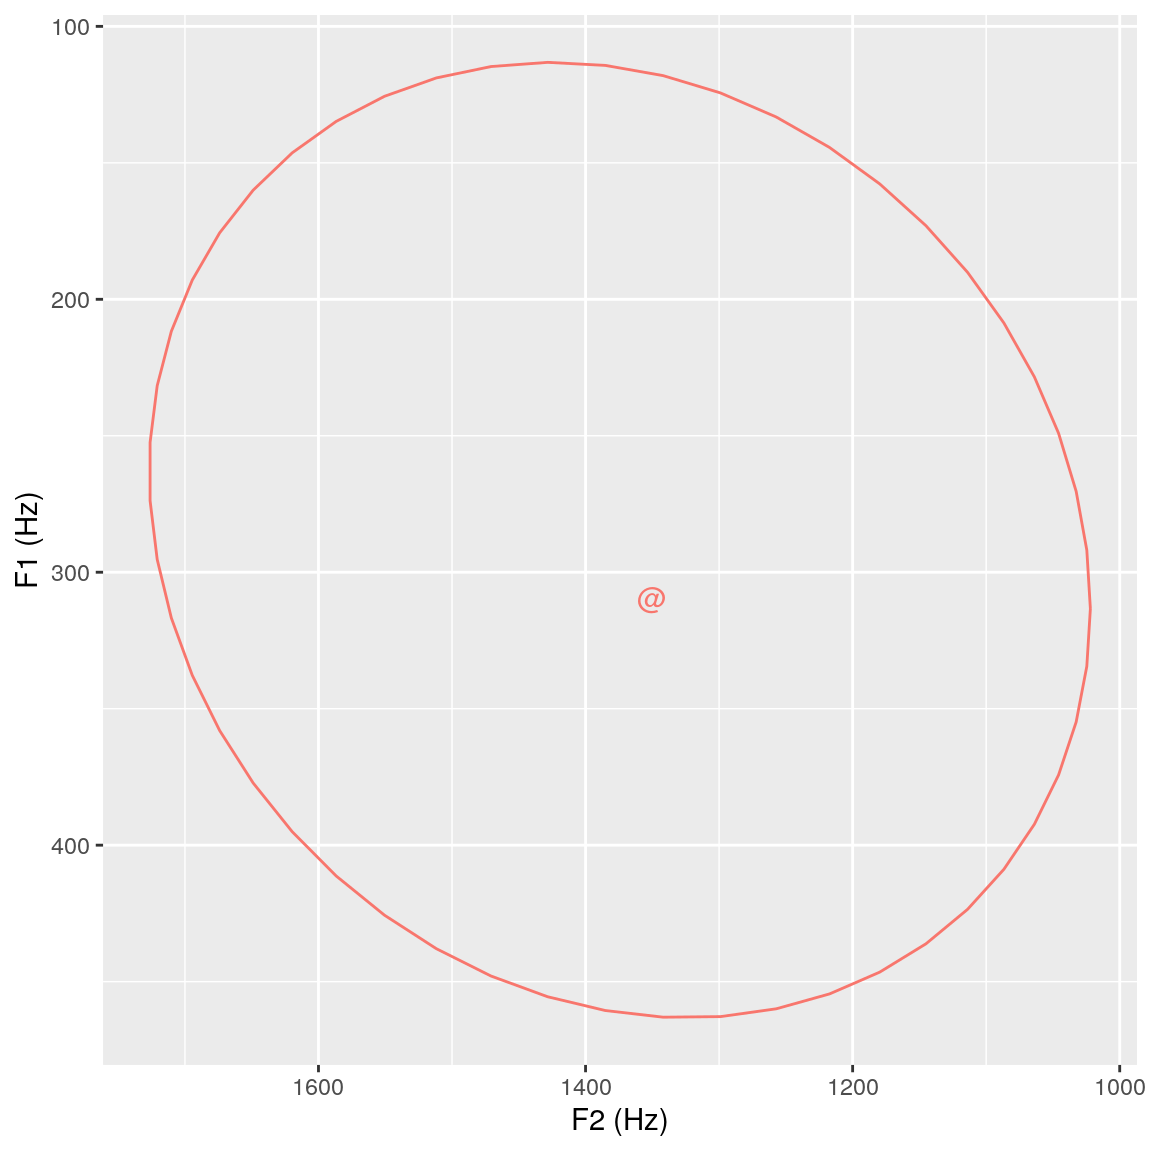
\includegraphics{tutorial_files/figure-latex/tutorial-eplot-1}

\}

\textbackslash{}caption\{95\% ellipse plot including centroid for F2 x F1 data extracted from the temporal midpoint of the vowel segments.\}\label{fig:tutorial-eplot}
\textbackslash{}end\{figure\}

Figure \ref{fig:tutorial-eplot} displays the first two formants extracted at the temporal midpoint of every \emph{@} vowel in \texttt{sl\_vowels}. The centroid of these formants is plotted on the F2 x F1 plane, and their 95\% ellipsis distribution is also shown. Although not necessarily applicable to the question posed at the beginning of this tutorial, the data exploration using the \texttt{dplyr} and \texttt{ggplot2} packages can be very helpful tools for providing an overview of the data at hand.

\hypertarget{vowel-height-as-a-function-of-word-types-content-vs.-function-evaluation-and-statistical-analysis}{%
\section{Vowel height as a function of word types (content vs.~function): evaluation and statistical analysis}\label{vowel-height-as-a-function-of-word-types-content-vs.-function-evaluation-and-statistical-analysis}}

The above data exploration only dealt with the actual \emph{@} vowels and disregarded the syllable type they occurred in. However, the question in the introduction of this chapter focuses on whether the \emph{@} vowel occurs in a content (labeled \emph{C}) or function (labeled \emph{F}) word. For data inspection purposes, the R code snippet below initially extracts the central 60\% (\texttt{filter()} conditions \texttt{times\_norm\ \textgreater{}=\ 0.2} and \texttt{times\_norm\ \textless{}=\ 0.8}) of the formant trajectories from \texttt{td\_vowels\_norm} using \texttt{dplyr} and displays them using \texttt{ggplot()}. It should be noted that before the call to \texttt{ggplot()} the labels of the \texttt{td\_vowels\_mid\_sec} are replaced with those of \texttt{sl\_word\_type}. This allows \texttt{ggplot()} to group the trajectories by their word type as opposed to their vowel labels as displayed in Figure \ref{fig:tutorial-dplotSylTyp}.

\begin{Shaded}
\begin{Highlighting}[]
\CommentTok{# extract central 60% from formant trajectories}
\NormalTok{td_vowels_mid_sec =}\StringTok{ }\NormalTok{td_vowels_norm }\OperatorTok\StringTok{ }
\StringTok{  }\KeywordTok{filter}\NormalTok{(times_norm }\OperatorTok{>=}\StringTok{ }\FloatTok{0.2}\NormalTok{, times_norm }\OperatorTok{<=}\StringTok{ }\FloatTok{0.8}\NormalTok{)}

\CommentTok{# replace labels with those of sl_word_type}
\NormalTok{td_vowels_mid_sec}\OperatorTok{$}\NormalTok{labels =}\StringTok{ }\NormalTok{sl_word_type}\OperatorTok{$}\NormalTok{labels[td_vowels_mid_sec}\OperatorTok{$}\NormalTok{sl_rowIdx]}

\KeywordTok{ggplot}\NormalTok{(td_vowels_mid_sec) }\OperatorTok{+}
\StringTok{  }\KeywordTok{aes}\NormalTok{(}\DataTypeTok{x =}\NormalTok{ times_norm, }\DataTypeTok{y =}\NormalTok{ T1, }\DataTypeTok{col =}\NormalTok{ labels, }\DataTypeTok{group =}\NormalTok{ labels) }\OperatorTok{+}
\StringTok{  }\KeywordTok{geom_smooth}\NormalTok{() }\OperatorTok{+}
\StringTok{  }\KeywordTok{labs}\NormalTok{(}\DataTypeTok{x =} \StringTok{"Duration (normalized)"}\NormalTok{, }\DataTypeTok{y =} \StringTok{"F1 (Hz)"}\NormalTok{) }
\end{Highlighting}
\end{Shaded}

\begin{verbatim}
## `geom_smooth()` using method = 'loess' and formula 'y ~ x'
\end{verbatim}

\textbackslash{}begin\{figure\}

\{\centering 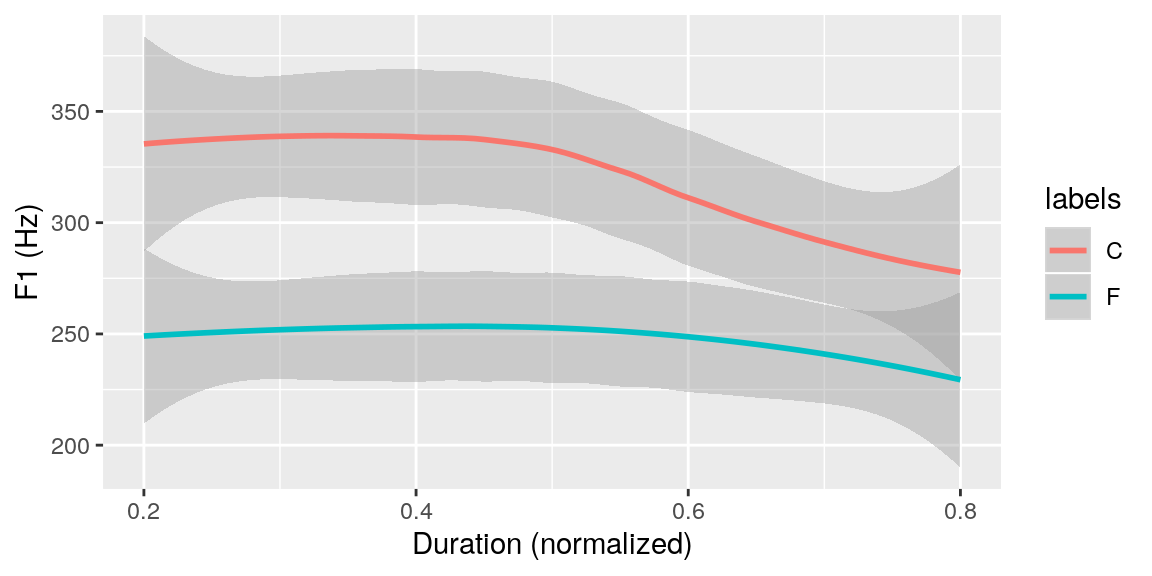
\includegraphics{tutorial_files/figure-latex/tutorial-dplotSylTyp-1}

\}

\textbackslash{}caption\{Ensemble averages of F1 contours of all tokens of the central 60\% of vowels grouped by word type (function (\emph{F}) vs.~content (\emph{W})).\}\label{fig:tutorial-dplotSylTyp}
\textbackslash{}end\{figure\}

As can be seen in Figure \ref{fig:tutorial-dplotSylTyp}, there seems to be a distinction in F1 trajectory height between vowels in content and function words. The following R snippet shows the code to produce a boxplot once again using the \texttt{ggplot2} package to further visually inspect the data (see Figure \ref{fig:tutorial-boxplot} for the plot produced by the below code).

\begin{Shaded}
\begin{Highlighting}[]
\CommentTok{# use group_by + summarise to calculate the means of the 60%}
\CommentTok{# formant trajectories}
\NormalTok{td_vowels_mid_sec_mean =}\StringTok{ }\NormalTok{td_vowels_mid_sec }\OperatorTok
\StringTok{  }\KeywordTok{group_by}\NormalTok{(sl_rowIdx) }\OperatorTok
\StringTok{  }\KeywordTok{summarise}\NormalTok{(}\DataTypeTok{labels =} \KeywordTok{unique}\NormalTok{(labels), }\DataTypeTok{meanF1 =} \KeywordTok{mean}\NormalTok{(T1))}


\CommentTok{# create boxplot using ggplot}
\KeywordTok{ggplot}\NormalTok{(td_vowels_mid_sec_mean, }\KeywordTok{aes}\NormalTok{(labels, meanF1)) }\OperatorTok{+}
\StringTok{  }\KeywordTok{geom_boxplot}\NormalTok{() }\OperatorTok{+}
\StringTok{  }\KeywordTok{labs}\NormalTok{(}\DataTypeTok{x =} \StringTok{"Word type"}\NormalTok{, }\DataTypeTok{y =} \StringTok{"mean F1 (Hz)"}\NormalTok{)}
\end{Highlighting}
\end{Shaded}

\begin{figure}

{\centering 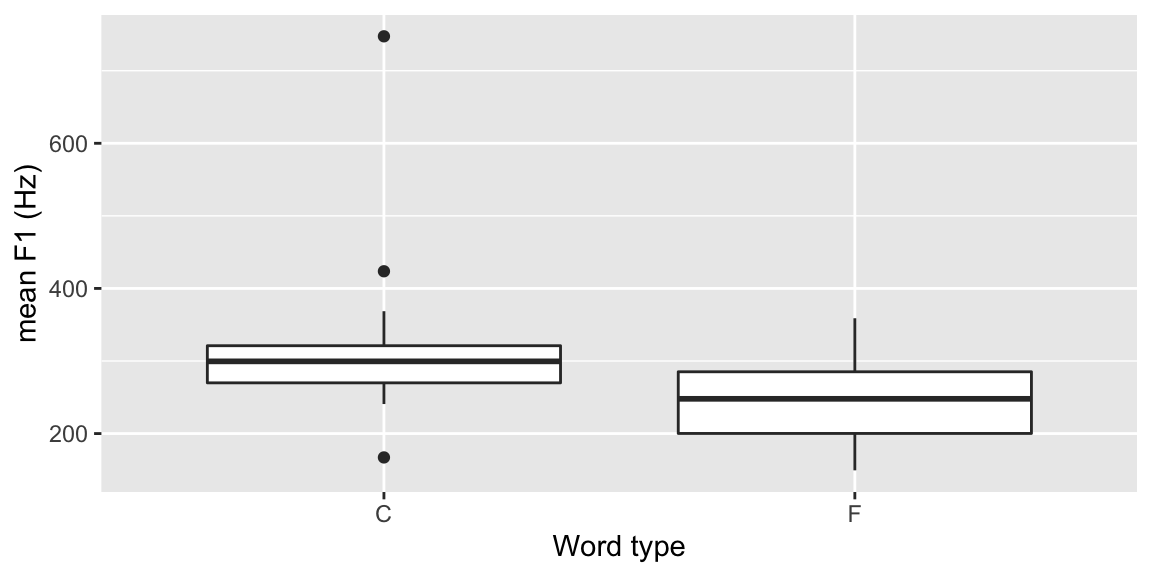
\includegraphics{tutorial_files/figure-latex/tutorial-boxplot-1} 

}

\caption{Boxplot produced using `ggplot2` to visualize the difference in F1 depending on whether the vowel occurs in content (*C*) or function (*F*) word.}\label{fig:tutorial-boxplot}
\end{figure}

To confirm or reject this, the following R code presents a very simple statistical analysis of the F1 mean values of the 60\% mid-section formant trajectories \footnote{It is worth noting that the sample size in this toy example is quite small. This obviously influences the outcome of the simple statistical analysis that is performed here.}. First, a Shapiro-Wilk test for normality of the distributions of the F1 means for both word types is carried out. As only one type is normally distributed, a Wilcoxon rank sum test is performed. The density distributions (commented out \texttt{plot()} function calls in the code below) are displayed in Figure \ref{fig:tutorial-stats1}.

\begin{Shaded}
\begin{Highlighting}[]
\CommentTok{# calculate density for vowels in function words}
\NormalTok{distrF =}\StringTok{ }\KeywordTok{density}\NormalTok{(td_vowels_mid_sec_mean[td_vowels_mid_sec_mean}\OperatorTok{$}\NormalTok{labels }\OperatorTok{==}\StringTok{ "F"}\NormalTok{,]}\OperatorTok{$}\NormalTok{meanF1)}

\CommentTok{# uncomment to visualize distribution}
\CommentTok{# plot(distrF)}

\CommentTok{# check that vowels in function}
\CommentTok{# words are normally distributed}
\KeywordTok{shapiro.test}\NormalTok{(td_vowels_mid_sec_mean[td_vowels_mid_sec_mean}\OperatorTok{$}\NormalTok{labels }\OperatorTok{==}\StringTok{ "F"}\NormalTok{,]}\OperatorTok{$}\NormalTok{meanF1)}
\end{Highlighting}
\end{Shaded}

\begin{verbatim}
## 
##  Shapiro-Wilk normality test
## 
## data:  td_vowels_mid_sec_mean[td_vowels_mid_sec_mean$labels == "F",     ]$meanF1
## W = 0.98618, p-value = 0.9868
\end{verbatim}

\begin{Shaded}
\begin{Highlighting}[]
\CommentTok{# p-value > 0.05 implying that the distribution}
\CommentTok{# of the data ARE NOT significantly different from}
\CommentTok{# normal distribution -> we CAN assume normality}

\CommentTok{# calculate density for vowels in content words}
\NormalTok{distrC =}\StringTok{ }\KeywordTok{density}\NormalTok{(td_vowels_mid_sec_mean[td_vowels_mid_sec_mean}\OperatorTok{$}\NormalTok{labels }\OperatorTok{==}\StringTok{ "C"}\NormalTok{,]}\OperatorTok{$}\NormalTok{meanF1)}

\CommentTok{# uncomment to visualize distribution}
\CommentTok{# plot(distrC)}

\CommentTok{# check that vowels in content}
\CommentTok{# words are normally distributed:}
\KeywordTok{shapiro.test}\NormalTok{(td_vowels_mid_sec_mean[td_vowels_mid_sec_mean}\OperatorTok{$}\NormalTok{labels }\OperatorTok{==}\StringTok{ "C"}\NormalTok{,]}\OperatorTok{$}\NormalTok{meanF1)}
\end{Highlighting}
\end{Shaded}

\begin{verbatim}
## 
##  Shapiro-Wilk normality test
## 
## data:  td_vowels_mid_sec_mean[td_vowels_mid_sec_mean$labels == "C",     ]$meanF1
## W = 0.67216, p-value = 1.819e-05
\end{verbatim}

\begin{Shaded}
\begin{Highlighting}[]
\CommentTok{# p-value < 0.05 implying that the distribution}
\CommentTok{# of the data ARE significantly different from}
\CommentTok{# normal distribution -> we CAN NOT assume normality}
\CommentTok{# (this somewhat unexpected result is probably}
\CommentTok{# due to the small sample size used in this toy example)}
\CommentTok{# -> use Wilcoxon rank sum test}

\CommentTok{# perform Wilcoxon rank sum test to establish}
\CommentTok{# whether vowel F1 depends on word type}
\KeywordTok{wilcox.test}\NormalTok{(meanF1 }\OperatorTok{~}\StringTok{ }\NormalTok{labels, }\DataTypeTok{data =}\NormalTok{ td_vowels_mid_sec_mean)}
\end{Highlighting}
\end{Shaded}

\begin{verbatim}
## 
##  Wilcoxon rank sum test
## 
## data:  meanF1 by labels
## W = 119, p-value = 0.04875
## alternative hypothesis: true location shift is not equal to 0
\end{verbatim}

\begin{figure}

{\centering 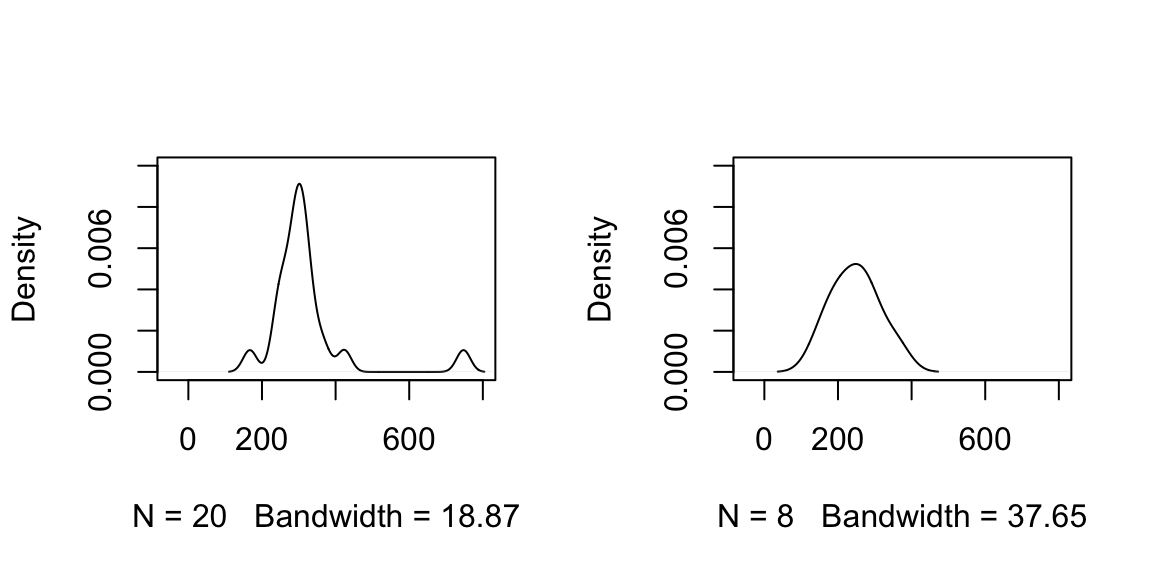
\includegraphics{tutorial_files/figure-latex/tutorial-stats1-1} 

}

\caption{Plots of density distributions of vowels in content words (left plot) and vowels in function words (right plot) of the above R code.}\label{fig:tutorial-stats1}
\end{figure}

As shown by the result of \texttt{wilcox.test()} in the above R code, word type (\emph{C} vs.~\emph{F}) has a significant influence on the vowel's F1 (W=121, p\textless{}0.05). Hence, the answer to the initially proposed question: \emph{Given an annotated speech database, is vowel height of the vowel @ (measured by its correlate, the first formant frequency) influenced by whether it appears in a content or function word?} is yes!

\hypertarget{conclusion}{%
\section{Conclusion}\label{conclusion}}

The tutorial given in this chapter gave an overview of what it is like working with the EMU-SDMS to try to solve a research question. As many of the concepts were only briefly explained, it is worth noting that explicit explanations of the various components and integral concepts are given in following chapters. Further, additional use cases that have been taken from the \texttt{emuR\_intro} vignette can be found in Appendix \ref{app-chap:useCases}. These use cases act as templates for various types of research questions and will hopefully aid the user in finding a solution similar to what she or he wishes to achieve.

\hypertarget{part-main-components-and-concepts}{%
\part{Main components and concepts}\label{part-main-components-and-concepts}}

\hypertarget{chap:annot-struct-mod}{%
\chapter[Annotation Structure Modeling ]{\texorpdfstring{Annotation Structure Modeling \footnote{Sections of this chapter where previously published in \citet{winkelmann:2017aa}}}{Annotation Structure Modeling }}\label{chap:annot-struct-mod}}

\begin{center}\includegraphics[width=0.75\linewidth]{pics/EMU-webAppEmu_annotStruct} \end{center}

The EMU-SDMS facilitates annotation structure modeling that surpasses that available in many other commonly used systems. This chapter provides an in-depth explanation of the annotation structure modeling capabilities the EMU-SDMS offers. One of the most common approaches for creating time-aligned annotations has been to differentiate between events that occur at a specific point in time but have no duration and segments that start at a point in time and have a duration. These annotation items are then grouped into time-ordered sets that are often referred to as tiers. As certain research questions benefit from different granularities of annotation, the timeline is often used to relate implicitly items from multiple tiers to each other as shown in Figure \ref{fig:annot-structhybridAnnot}A. While sufficient for single or unrelated tier annotations, we feel this type of representation is not suitable for more complex annotation structures, as it results in unnecessary, redundant data and data sets that are often difficult to analyze. This is because there are no explicit relationships between annotation items, and it is often necessary to introduce error tolerance values to analyze slightly misaligned time values to find relationships iteratively over multiple levels. The main reason for the prevalence of this sub-optimal strategy is largely because the available software tools (e.g., Praat by \citet{boersma:2011a}) do not permit any other forms of annotations. These widely used annotation tools often only permit the creation and manipulation of segment and event tiers which in turn has forced users to model their annotation structures on these building blocks alone.

Linguists who deal with speech and language on a purely symbolic level tend to be more familiar with a different type of annotation structure modeling. They often model their structures in the form of a vertically oriented, directed acyclic graph that, but for a few exceptions that are needed for things like elision modeling (e.g., the /ɪ/ elision that may occur between the canonical representation of the word \emph{family} /fæmɪli/ and its phonetic representation {[}fæmli{]}), loosely adheres to the formal definition of a tree in the graph-theoretical sense (\citet{knuth:ar1968a}) as depicted in Figure \ref{fig:annot-structhybridAnnot}B. While this form of modeling explicitly defines relationships between annotation items (represented by dashed lines in Figure \ref{fig:annot-structhybridAnnot}B), it lacks the ability to map these items to the timeline and therefore the matching speech signal.

\begin{figure}

{\centering 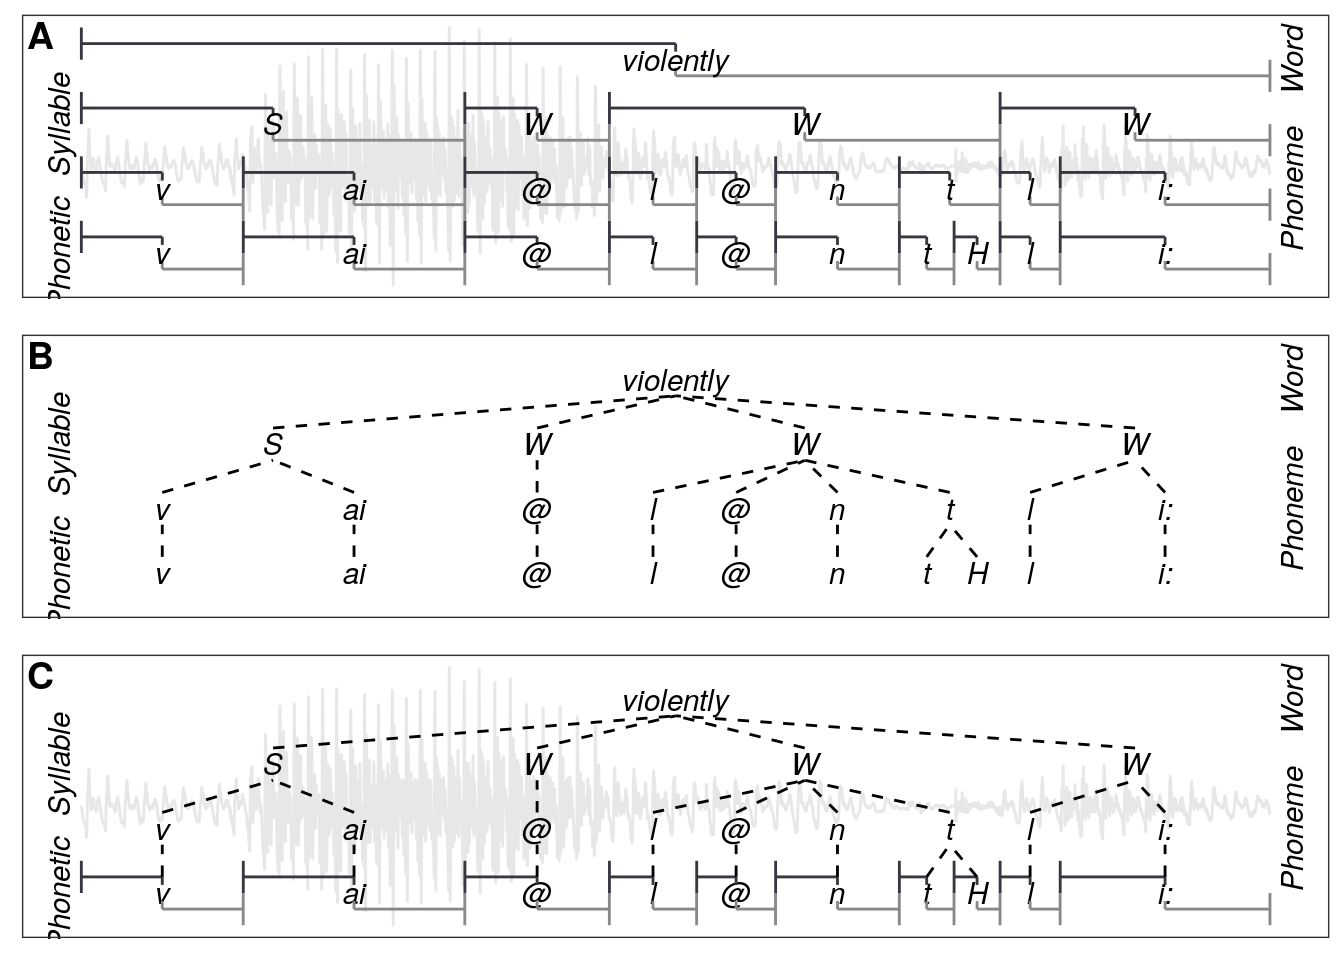
\includegraphics[width=1\linewidth,keepaspectratio]{annot_struct_files/figure-latex/annot-structhybridAnnot-1} 

}

\caption{**A:** a purely time-aligned annotation; **B:** a purely timeless, symbolic annotation; **C:** a time-aligned hierarchical annotation.}\label{fig:annot-structhybridAnnot}
\end{figure}

To our knowledge, the legacy EMU system (\citet{cassidy:sc2001a}) and its predecessors (e.g., \citet{harrington:csl1993a}) were the first to fuse pragmatically purely time-aligned and symbolic tree-like annotations. This was achieved by providing software tools that allowed for these types of annotation structures to be generated, queried and evaluated. In practice, each annotation item had its own unique identifier within the annotation. These unique IDs could then be used to reference each individual item and link them together using dominance relations to form the hierarchical annotation structure. On the one hand, this dominance relation implies the temporal inclusion of the linked sub-level items and was partially predicated on the \emph{no-crossing constraint} as described in \citet{coleman:lp1991a}). This constraint does not permit the crossing of dominance relationships with respect to their sequential ordering (see also Section 4.2 of \citet{cassidy:sc2001a}). Since the dominance relations imply temporal inclusion, events can only be children in a parent-child relationship. To allow for timeless annotation items, a further timeless level type was used to complement the segment and event type levels used for time-aligned annotations. Each level of annotation items was stored as an ordered set to ensure the sequential integrity of both the time-aligned and timeless item levels. The legacy system also reduced data redundancy by allowing parallel annotations to be defined in the form of linearly linked levels for any given level (e.g., a segment level bearing SAMPA annotations as well as IPA UTF-8 annotations).

The new EMU-SDMS has adopted some concepts of the legacy system in that levels of type \texttt{SEGMENT} and \texttt{EVENT} contain annotation items with labels and time information, similar to the tiers known from other software tools such as Praat, while levels of type \texttt{ITEM} are timeless and contain annotation items with labels only. \texttt{SEGMENT} and \texttt{EVENT} levels differ in that units at the \texttt{SEGMENT}s level have a start time and a duration, while units at the \texttt{EVENT} level contain a single time point only. Additionally, every annotation item is able to contain multiple labels and has a unique identifier which is used to link items across levels. These building blocks provide the user with a general purpose annotation modeling tool that allows complex annotation structures to be modeled that best represent the data. An example of a time-aligned hierarchical annotation is depicted in Figure \ref{fig:annot-structhybridAnnot}C, which essentially combines the annotation of Figure \ref{fig:annot-structhybridAnnot}B with the most granular time-bearing level (i.e.~the \emph{``Phonetic''} level) of Figure \ref{fig:annot-structhybridAnnot}A.

In accordance with other approaches (among others see \citet{bird:sc2001a}, \citet{zipser:2010a}, \citet{ide:nle2004a}), the EMU-SDMS annotation structure can be viewed as a graph that consists of three types of nodes (\texttt{EVENT}s, \texttt{SEGMENT}s, \texttt{ITEM}s) and two types of relations (\texttt{dominance} and \texttt{sequence}) which are directed, transitive and indicate the dominance and sequential relationships between nodes of the graph. As was shown in a pseudo-code example that converted an Annotation Graph (\citet{bird:sc2001a}) into the legacy EMU annotation format in \citet{cassidy:sc2001a}, these formats can be viewed as conceptually equivalent sub- or super-set representations of each other. This has also been shown by developments of meta models with independent data representation such as \texttt{Salt} (\citet{zipser:2010a}), which enable abstract internal representations to be derived that can be exported to equal-set or super-set formats without the loss of information. We therefore believe that the decision as to which data format serializations are used by a given application should be guided by the choice of technology and the target audience or research field. This is consistent with the views of the committee for the Linguistic Annotation Framework (LAF) who explicitly state in the ISO CD 24612 (LAF) document (\citet{ISOLAF});

\begin{quote}
Although the LAF pivot format may be used in any context, it is assumed that users will represent annotations using their own formats, which can then be transduced to the LAF pivot format for the purposes of exchange, merging and comparison.
\end{quote}

The transduction of an EMU annotation into a format such as the LAF pivot format is a simple process, as they share many of the same concepts and are well defined formats.

\hypertarget{per-database-annotation-structure-definition}{%
\section{Per database annotation structure definition}\label{per-database-annotation-structure-definition}}

Unlike other systems, the EMU-SDMS requires the user to define the annotation structure formally for all annotations within a database. Much as Document Type Definition (DTD) or XML Schema Definition (XSD) describe the syntactically valid elements in an Extensible Markup Language (XML) document, the database configuration file of an \texttt{emuDB} defines the valid annotation levels and therefore the type of items that are allowed to be present in a database. Unlike DTDs or XSDs, the configuration file can also define semantic relationships between annotation levels which fall outside the scope of traditional, syntactically oriented schema definitions and validation. This global definition of an annotation structure has numerous benefits for the data integrity of the database, as the EMU-SDMS can perform consistency checks and prevent malformed as well as semantically void annotation structures \footnote{Although the consistency is ensured by the \texttt{EMU-SDMS} while annotation editing operations are performed, currently no actual consistency checks are performed while loading or saving an annotation. However, we plan to add this functionality in future releases.}. Because of these formal definitions, the EMU system generally distinguishes between the actual representations of a structural element which are contained within the database and their formal definitions. An example of an actual representation, that is a subset of the actual annotation, would be a level contained in an annotation file that contains \texttt{SEGMENT}s that annotate a recording. The corresponding formal definition would be a level definition entry in the database's configuration file, which specifies and validates the level's existence within the database.

As mentioned above, the actual annotation files of an \texttt{emuDB} contain the annotation items as well as their hierarchical linking information. To be able to check the validity of a connection between two items, the user specifies which links are permitted for the entire database just as for the level definitions. The permitted hierarchical relationships in an \texttt{emuDB} are expressed through link definitions between level definitions as part of the database configuration. There are three types of valid hierarchical relationships between levels: \texttt{ONE\_TO\_MANY}, \texttt{MANY\_TO\_MANY} and \texttt{ONE\_TO\_ONE}. These link definitions specify the permitted relationships between instances of annotation items of one level and those of another. The structure of the hierarchy that corresponds to the annotation depicted in Figure \ref{fig:annot-structhybridAnnot}C can be seen in Figure \ref{fig:annotStruct}A. The structure in Figure \ref{fig:annotStruct}A is a typical example of an EMU hierarchy where only the \textit{Phonetic} level of type \texttt{SEGMENT} contains time information and the others are timeless as they are of the type \texttt{ITEM}. The top three levels, \emph{Text}, \emph{Syllable} and \emph{Phoneme}, have a \texttt{ONE\_TO\_MANY} relationship specifying that a single item in the parent level may have a dominance relationship with multiple items in the child level. In this example, the relationship between \textit{Phoneme} and \emph{Phonetic} is \texttt{MANY\_TO\_MANY}: this type of relationship can be used to represent schwa elision and subsequent sonorant syllabification, as when the final syllable of \emph{sudden} is \emph{\href{mailto:d@n}{\nolinkurl{d@n}}} at the \emph{Phoneme} level but \emph{dn} at the \emph{Phonetic} level. Figure \ref{fig:annotStruct}B displays an example of a more complex, intersecting hierarchical structure definition where Abercrombian feet (\citet{abercombie:1967a}) are incorporated into the tones and break indices (ToBI) (\citet{beckman:1997aa}) prosodic hierarchy by allowing an intonational phrase to be made up of one or more feet (for further details see \citet{harrington:2010a} page 98).

\begin{figure}

{\centering \includegraphics[width=0.75\linewidth]{pics/annotStruct} 

}

\caption{**A:** a schematic representation of the hierarchical structure of an `emuDB` that corresponds to the annotation depicted in figure 4.1C; **B:** example of a more complex, intersecting hierarchical structure.}\label{fig:annotStruct}
\end{figure}

Based on our experience, the explicit definition of the annotation structure for every database which was also integral to the legacy system addresses the excessively expressive nature of annotational modeling systems mentioned in \citet{bird:sc2001a}. Although, in theory, infinitely large hierarchies can be defined for a database, users of the legacy system typically chose to use only moderately complex annotation structures. The largest hierarchy definitions we have encountered spanned up to fifteen levels while the average amount of levels was between three and five. This self-restriction is largely due to the primary focus of speech and spoken language domain-specific annotations, as the number of annotation levels between chunks of speech above the word level (intonational phrases/sentences/turns/etc.) and the lower levels (phonetic segmentation/EMA gestural landmark annotation/tone annotation/etc.) is a finite set.

\hypertarget{parallel-labels-and-multiple-attributes}{%
\section{Parallel labels and multiple attributes}\label{parallel-labels-and-multiple-attributes}}

The legacy EMU system made a distinction between linearly and non-linearly linked inter-level links. Linearly linked levels were used to describe, enrich or supplement another level. For example, a level called \emph{Category} might have been included as a separate level from \emph{Word} for marking words' grammatical category memberships (thus each word might be marked as one of adjective, noun, verb, etc.), or information about whether or not a syllable is stressed might be included on a separate \emph{Stress} tier (description taken from \citet{harrington:2010a} page 77). Using \texttt{ONE\_TO\_ONE} link definitions to define a relationship between two levels, it is still possible to model linearly linked levels in the new EMU-SDMS. However, an additional, cleaner concept that reduces the extra level overhead has been implemented that allows every annotation item to carry multiple attributes (i.e., labels). Further, using this construct reduces the number of levels, items and links and therefore the hierarchical complexity of an annotation. The generic term ``attribute'' (vs.~``label'') was chosen to have the flexibility of adding attributes that are not of the type \texttt{STRING} (i.e., labels) to the annotation modeling capabilities of the EMU-SDMS in future versions. Figure \ref{fig:paraLabels} shows the annotation structure modeling difference between linearly linked levels (see Figure \ref{fig:paraLabels}A) and an annotation structure using multiple attributes (see Figure \ref{fig:paraLabels}B). Figure \ref{fig:paraLabels}A shows three separate levels (\emph{Word}, \emph{Accent} and \emph{Text}) that have a \texttt{ONE\_TO\_ONE} relationship. Each of their annotation items is linked to exactly one annotation item in the child level (e.g., \emph{A1-A3}). Figure \ref{fig:paraLabels}B shows a single level that has three attribute definitions (\emph{Word}, \emph{Accent} and \emph{Text}) and each annotation item contains three attributes (e.g., \emph{A1-A3}).

\begin{figure}

{\centering \includegraphics[width=0.75\linewidth]{pics/annotStruct} 

}

\caption{Schematic representation of annotation structure modeling difference between **A:** linearly linked levels and **B:** an annotation structure using multiple attributes.}\label{fig:paraLabels}
\end{figure}

It is worth noting that every level definition must have an attribute definition which matches its level name. This primary attribute definition must also be present in every annotation item belonging to a level. As \texttt{emuR}'s database interaction functions, such as \texttt{add\_levelDefinition()}, and the \texttt{EMU-webApp} automatically perform the necessary actions this should only be of interest to (semi-)advanced users wishing to automatically generate the \texttt{\_annot.json} format.

\hypertarget{metadata-strategy-using-single-bundle-root-nodes}{%
\section{Metadata strategy using single bundle root nodes}\label{metadata-strategy-using-single-bundle-root-nodes}}

As the legacy EMU system and the new EMU-SDMS do not have an explicit method for storing metadata associated with bundles\footnote{Future versions of \texttt{emuR} may allow \texttt{\_meta.json} files containing meta information in the form of key-value pairs to be placed in either the \texttt{\_emuDB}, the \texttt{\_ses} or the \texttt{\_bndl} directories.}, over the years an annotation structure convention has been developed to combat this issue. The convention is to use a generic top level (often simply called \texttt{bundle}) that contains a single annotation item in every annotation file. Using the multiple attribute annotation structure modeling capability of the EMU-SDMS, this single annotation item can hold any meta data associated with the bundle. Additionally linking the item to all the annotation items of its child level effectively makes it a parent to every item of the hierarchy. This linking information can later be exploited to query only bundles with matching meta data (see Chapter \ref{chap:querysys} for details). Figure \ref{fig:singleBundleRootNode} displays a hierarchical annotation where the top level (\texttt{bundle}) contains information about the speaker's \texttt{gender}, the city of birth (\texttt{COB}) and \texttt{age}.

\begin{figure}

{\centering \includegraphics[width=0.65\linewidth]{pics/singleBundleRootNode} 

}

\caption{Hierarchical annotation displaying single bundle root node metadata strategy where the label of the primary attribute definition (*bundle*) is empty, *gender* encodes the speaker's gender, *COB* encodes the speakers city of birth and *age* encodes the speaker's age in the form of a string.}\label{fig:singleBundleRootNode}
\end{figure}

\hypertarget{conclusion-1}{%
\section{Conclusion}\label{conclusion-1}}

The annotation structure modeling capabilities of the EMU-SDMS surpass those of many other commonly used systems. They do so by not only allowing the use of levels containing time information (levels of type \texttt{SEGMENT} and \texttt{EVENT}) but also timeless levels (levels of type \texttt{ITEM}). Additionally, they allow users to define hierarchical annotation structures by allowing explicit links to be implemented from one level's items to those of another. Although it is not obligatory to use them in the EMU-SDMS, we feel the usage of hierarchical annotations allow for complex rich data modeling and are often cleaner representations of the annotations at hand.

\hypertarget{chap:emuDB}{%
\chapter[The \texttt{emuDB} Format ]{\texorpdfstring{The \texttt{emuDB} Format \footnote{Sections of this chapter where published in \citet{winkelmann:2017aa} and some examples taken from the \texttt{emuDB} vignette of the \texttt{emuR} package.}}{The emuDB Format }}\label{chap:emuDB}}

\begin{center}\includegraphics[width=0.75\linewidth]{pics/EMU-webAppEmu_emuDB} \end{center}

This chapter describes the \texttt{emuDB} format, which is the new database format of the EMU-SDMS, and shows how to create and interact with this format. The \texttt{emuDB} format is meant as a simple, general purpose way of storing speech databases that may contain complex, rich, hierarchical annotations as well as derived and complementary speech data. These different components will be described throughout this chapter, and examples will show how to generate and manipulate them. On designing the new EMU system, considerable effort went into designing an appropriate database format. We needed a format that was standardized, well structured, easy to maintain, easy to produce, easy to manipulate and portable.

We decided on the JavaScript Object Notation (JSON) file format\footnote{JSON schema files available here \url{https://github.com/IPS-LMU/EMU-webApp/tree/master/dist/schemaFiles}} as our primary data source for several reasons. It is simple, standardized, widely-used and text-based as well as machine and human readable. In addition, this portable text format allows expert users to (semi-) automatically process and/or generate annotations. Other tools such as the BAS Webservices \citep{kisler:2012a} and SpeechRecorder \citep{draxler:2004a} have already taken advantage of being able to produce such annotations. Using database back-end options such as relational or graph databases of either the SQL or NoSQL variety as the primary data source for annotations would not directly permit other tools to produce annotations because intermediary exchange file formats would have to be defined to permit this functionality with these back-ends. Our choice of the JSON format was also guided by the decision to incorporate web technologies as part of the EMU-SDMS for which the JSON format is the de facto standard (see Chapter \ref{chap:emu-webApp}). Further, as the default encoding of the JSON format is UTF-8 the EMU-SDMS fully supports the Unicode character set for any user-defined string within an \texttt{emuDB} (e.g.~level names and labels)\footnote{According to the JSON specification (see \url{https://json.org/}) the only characters that have to be escaped within a JSON string are: '' (as this marks the start/end of a string), \textbackslash{} (as this is the escape character) or control-characters (\textbackslash{}b = backspace, \textbackslash{}f = form feed, \textbackslash{}n = new line, \textbackslash{}r = carriage return, \textbackslash{}t = tab). Unicode characters in their hexadecimal form using the \textbackslash{}u followed by for-hex-digits may also be used.}.

We chose to use the widely adopted Waveform Audio File Format (\texttt{WAVE}, or more commonly known as \texttt{WAV} due to its filename extension) as our primary media/audio format. Although some components of the EMU-SDMS, notably the \texttt{wrassp} package, can handle various other media/audio formats (see \texttt{?wrassp::AsspFileFormats} for details) this is the only audio file format currently supported by every component of the EMU-SDMS. Nevertheless, the \texttt{wrassp} package can be utilized to convert files from one of it's other supported file formats to the \texttt{WAV} format \footnote{However, if things like resampeling are required we suggest using other tools such as the freely available Sound eXchange (SoX) command line tool (see \url{http://sox.sourceforge.net/}) to perform these operation}. Future releases of the EMU-SDMS might include the support of other media/audio formats.

In contrast to other systems, including the legacy EMU system, we chose to fully standardize the on-disk structure of speech databases with which the system is capable of working. This provides a standardized and structured way of storing speech databases while providing the necessary amount of freedom and separability to accommodate multiple types of data. Further, this standardization enables fast parsing and simplification of file-based error tracking and simplifies database subset and merging operations as well as database portability. An overview of all database interaction functions is given in Section \ref{sec:emuRpackageDetails-emuDBinteract}.

\hypertarget{database-design}{%
\section{Database design}\label{database-design}}

An \texttt{emuDB} consists of a set of files and directories that adhere to a certain structure and naming convention (see Figure \ref{fig:schematic-emuDB-structure}). The database root directory must include a single \texttt{\_DBconfig.json} file that contains the configuration options of the database such as its level definitions, how these levels are linked in the database hierarchy and how the data is to be displayed by the graphical user interface. A detailed description of the \texttt{\_DBconfig.json} file is given in Appendix \ref{subsec:app-chapFileFormatsDBconfig}. The database root directory also contains arbitrarily named session directories (except for the obligatory \texttt{\_ses} suffix). These session directories can be used to group the recordings of a database in a logical manner. Sessions can be used, for example, to group all recordings from speaker \texttt{AAA} into a session called \texttt{AAA\_ses}.

\begin{figure}

{\centering \includegraphics[width=0.65\linewidth]{pics/db_structure} 

}

\caption{Schematic `emuDB` file and directory structure.}\label{fig:schematic-emuDB-structure}
\end{figure}

Each session directory can contain any number of \texttt{\_bndl} directories (e.g., \texttt{rec1\_bndl} \texttt{rec2\_bndl} \ldots{} \texttt{rec9\_bndl}). All files belonging to a recording (i.e., all files describing the same timeline) are stored in the same bundle directory. This includes the actual recording (\texttt{.wav}) and can contain optional derived or supplementary signal files in the simple signal file format (SSFF) \citep{cassidy:2013a} such as formants (\texttt{.fms}) or the fundamental frequency (\texttt{.f0}), both of which can be calculated using the \texttt{wrassp} package (see Chapter \ref{chap:wrassp}). Each bundle directory contains the annotation file (\texttt{\_annot.json}) of that bundle (i.e., the annotations and the hierarchical linking information; see Appendix \ref{subsec:app-chapFileFormatsAnnotJSON} for a detailed description of the file format). JSON schema files for all the JSON files types used have been developed to ensure the syntactic integrity of the database (see \url{https://github.com/IPS-LMU/EMU-webApp/tree/master/dist/schemaFiles}). All files within a bundle that are associated with that bundle must have the same basename as the \texttt{\_bndl} directory prefix. For example, the signal file in bundle \texttt{rec1\_bndl} must have the name \texttt{rec1.wav} to be recognized as belonging to the bundle. The optional \texttt{\_emuDBcache.sqlite} file in the root directory (see Figure \ref{fig:schematic-emuDB-structure} contains the relational cache representation of the annotations of the \texttt{emuDB} (see Chapter \ref{chap:querysys-impl} for further details). All files in an \texttt{\_bndl} directory that do not follow the above naming conventions will simply be ignored by the database interaction functions of the \texttt{emuR} package.

\hypertarget{creating-an-emudb}{%
\section{\texorpdfstring{Creating an \texttt{emuDB}}{Creating an emuDB}}\label{creating-an-emudb}}

The two main strategies for creating \texttt{emuDB}s are either to convert existing databases or file collections to the new format or to create new databases from scratch where only \texttt{.wav} audio files are present. Chapter \ref{chap:tutorial} gave an example of how to create an \texttt{emuDB} from an existing TextGrid file collection and other conversion routines are covered in Section \ref{sec:emuRpackageDetails-importRoutines}. In this chapter we will focus on creating an \texttt{emuDB} from scratch with nothing more than a set of \texttt{.wav} audio files present.

\hypertarget{creating-an-emudb-from-scratch}{%
\subsection{\texorpdfstring{Creating an \texttt{emuDB} from scratch}{Creating an emuDB from scratch}}\label{creating-an-emudb-from-scratch}}

The R code snippet below shows how an empty \texttt{emuDB} is created in the directory provided by R's \texttt{tempdir()} function. As can be seen by the output of the \texttt{list.files()} function, \texttt{create\_emuDB()} creates a directory containing a \texttt{\_DBconfig.json} file only.

\begin{Shaded}
\begin{Highlighting}[]
\CommentTok{# load package}
\KeywordTok{library}\NormalTok{(emuR, }\DataTypeTok{warn.conflicts =}\NormalTok{ F)}

\CommentTok{# create demo data in directory }
\CommentTok{# provided by tempdir()}
\KeywordTok{create_emuRdemoData}\NormalTok{(}\DataTypeTok{dir =} \KeywordTok{tempdir}\NormalTok{())}

\CommentTok{# create emuDB called "fromScratch"}
\CommentTok{# (verbose = F is only set to avoid additional output in manual)}
\KeywordTok{create_emuDB}\NormalTok{(}\DataTypeTok{name =} \StringTok{"fromScratch"}\NormalTok{,}
             \DataTypeTok{targetDir =} \KeywordTok{tempdir}\NormalTok{(),}
             \DataTypeTok{verbose =}\NormalTok{ F)}

\CommentTok{# generate path to the empty fromScratch created above}
\NormalTok{dbPath =}\StringTok{ }\KeywordTok{file.path}\NormalTok{(}\KeywordTok{tempdir}\NormalTok{(), }\StringTok{"fromScratch_emuDB"}\NormalTok{)}

\CommentTok{# show content of empty fromScratch emuDB}
\KeywordTok{list.files}\NormalTok{(dbPath)}
\end{Highlighting}
\end{Shaded}

\begin{verbatim}
## [1] "fromScratch_DBconfig.json"
\end{verbatim}

\hypertarget{loading-and-editing-an-empty-database}{%
\subsection{Loading and editing an empty database}\label{loading-and-editing-an-empty-database}}

The initial step in manipulating and generally interacting with a database is to load the database into the current R session. The R code below shows how to load the \emph{fromScratch} database and shows the empty configuration by displaying the output of the \texttt{summary()} function.

\begin{Shaded}
\begin{Highlighting}[]
\CommentTok{# load database}
\CommentTok{# (verbose = F is only set to avoid additional output in manual)}
\NormalTok{dbHandle =}\StringTok{ }\KeywordTok{load_emuDB}\NormalTok{(dbPath, }\DataTypeTok{verbose =}\NormalTok{ F)}

\CommentTok{# show summary of dbHandle}
\KeywordTok{summary}\NormalTok{(dbHandle)}
\end{Highlighting}
\end{Shaded}

\begin{verbatim}
## Name:     fromScratch 
## UUID:     ab400a00-1a65-4007-ab13-3c52a68d832c 
## Directory:    /private/var/folders/yk/8z9tn7kx6hbcg_9n4c1sld980000gn/T/RtmpvpkoCG/fromScratch_emuDB 
## Session count: 0 
## Bundle count: 0 
## Annotation item count:  0 
## Label count:  0 
## Link count:  0 
## 
## Database configuration:
## 
## SSFF track definitions:
## NULL
## 
## Level definitions:
## NULL
## 
## Link definitions:
## NULL
\end{verbatim}

\begin{Shaded}
\begin{Highlighting}[]
\CommentTok{# show class vector of dbHandle}
\KeywordTok{class}\NormalTok{(dbHandle)}
\end{Highlighting}
\end{Shaded}

\begin{verbatim}
## [1] "emuDBhandle"
\end{verbatim}

As can be seen in the above R code example, the class of a loaded \texttt{emuDB} is \texttt{emuDBhandle}. A \texttt{emuDBhandle} object is used to reference a loaded \texttt{emuDB} in the database interaction functions of the \texttt{emuR} package. In this chapter we will show how to use this \texttt{emuDBhandle} object to perform database manipulation operations. Most of the \texttt{emuDB} manipulation functions follow the following function prefix naming convention:

\begin{itemize}
\tightlist
\item
  \texttt{add\_XXX} add a new instance of \texttt{XXX} / \texttt{set\_XXX} set the current instance of \texttt{XXX},
\item
  \texttt{list\_XXX} list the current instances of \texttt{XXX} / \texttt{get\_XXX} get the current instance of \texttt{XXX},
\item
  \texttt{remove\_XXX} remove existing instances of \texttt{XXX}.
\end{itemize}

\hypertarget{level-definitions}{%
\subsection{Level definitions}\label{level-definitions}}

Unlike other systems, the EMU-SDMS requires the user to formally define the annotation structure for the entire database. An essential structural element of any \texttt{emuDB} are its levels. A level is a more general term for what is often referred to as a tier. It is more general in the sense that people usually expect tiers to contain time information. Levels can either contain time information if they are of the type \texttt{EVENT} or of the type \texttt{SEGMENT} but are timeless if they are of the type \texttt{ITEM} (see Chapter \ref{chap:annot-struct-mod} for further details). It is also worth noting that an \texttt{emuDB} distinguishes between the definition of an annotation structure element and the actual annotations. The definition of an annotation structure element such as a level definition is merely an entry in the \texttt{\_DBconfig.json} file which specifies that this level is allowed to be present in the \texttt{\_annot.json} files. The levels that are present in an \texttt{\_annot.json} file, on the other hand, have to adhere to the definitions in the \texttt{\_DBconfig.json}.

As the \emph{fromScratch} database (already loaded) does not contain any annotation structural element definitions, the R code snippet below shows how a new level definition called \emph{Phonetic} of type \texttt{SEGMENT} is added to the \texttt{emuDB}.

\begin{Shaded}
\begin{Highlighting}[]
\CommentTok{# show no level definitions}
\CommentTok{# are present}
\KeywordTok{list_levelDefinitions}\NormalTok{(dbHandle)}
\end{Highlighting}
\end{Shaded}

\begin{verbatim}
## NULL
\end{verbatim}

\begin{Shaded}
\begin{Highlighting}[]
\CommentTok{# add level defintion}
\KeywordTok{add_levelDefinition}\NormalTok{(dbHandle,}
                    \DataTypeTok{name =} \StringTok{"Phonetic"}\NormalTok{,}
                    \DataTypeTok{type =} \StringTok{"SEGMENT"}\NormalTok{)}

\CommentTok{# show newly added level definition}
\KeywordTok{list_levelDefinitions}\NormalTok{(dbHandle)}
\end{Highlighting}
\end{Shaded}

\begin{verbatim}
##       name    type nrOfAttrDefs attrDefNames
## 1 Phonetic SEGMENT            1    Phonetic;
\end{verbatim}

The example below shows how a further level definition is added that will contain the orthographic word transcriptions for the words uttered in our recordings. This level will be of the type \texttt{ITEM}, meaning that elements contained within the level are sequentially ordered but do not contain any time information.

\begin{Shaded}
\begin{Highlighting}[]
\CommentTok{# add level definition}
\KeywordTok{add_levelDefinition}\NormalTok{(dbHandle,}
                    \DataTypeTok{name =} \StringTok{"Word"}\NormalTok{,}
                    \DataTypeTok{type =} \StringTok{"ITEM"}\NormalTok{)}

\CommentTok{# list newly added level definition}
\KeywordTok{list_levelDefinitions}\NormalTok{(dbHandle)}
\end{Highlighting}
\end{Shaded}

\begin{verbatim}
##       name    type nrOfAttrDefs attrDefNames
## 1 Phonetic SEGMENT            1    Phonetic;
## 2     Word    ITEM            1        Word;
\end{verbatim}

The function \texttt{remove\_levelDefinition()} can also be used to remove unwanted level definitions. However, as we wish to further use the levels \emph{Phonetic} and \emph{Word}, we will not make use of this function here.

\hypertarget{attribute-definitions}{%
\subsubsection{Attribute definitions}\label{attribute-definitions}}

Each level definition can contain multiple attributes, the most common, and currently only supported attribute being a label (of type \texttt{STRING}). Thus it is possible to have multiple parallel labels (i.e., attribute definitions) in a single level. This means that a single annotation item instance can contain multiple labels while sharing other properties such as the start and duration information. This can be useful when modeling certain types of data. An example of this would be the \emph{Phonetic} level created above. It is often the case that databases contain both the phonetic transcript using IPA UTF-8 symbols as well as a transcript using Speech Assessment Methods Phonetic Alphabet (SAMPA) symbols. To avoid redundant time information, both of these annotations can be stored on the same \texttt{Phonetic} level using multiple attribute definitions (i.e., parallel labels). The next R code snippet shows the current attribute definitions of the \texttt{Phonetic} level.

\begin{Shaded}
\begin{Highlighting}[]
\CommentTok{# list attribute definitions of 'Phonetic' level}
\KeywordTok{list_attributeDefinitions}\NormalTok{(dbHandle,}
                          \DataTypeTok{levelName =} \StringTok{"Phonetic"}\NormalTok{)}
\end{Highlighting}
\end{Shaded}

\begin{verbatim}
##       name    level   type hasLabelGroups hasLegalLabels
## 1 Phonetic Phonetic STRING          FALSE          FALSE
\end{verbatim}

Even though no attribute definition has been added to the \texttt{Phonetic} level, it already contains an attribute definition that has the same name as its level. This attribute definition represents the obligatory primary attribute of that level. As every level must contain an attribute definition that has the same name as its level, it is automatically added by the \texttt{add\_levelDefinition()} function. To follow the above example, the next R code snippet adds a further attribute definition to the \texttt{Phonetic} level that contains the SAMPA versions of our annotations.

\begin{Shaded}
\begin{Highlighting}[]
\CommentTok{# add}
\KeywordTok{add_attributeDefinition}\NormalTok{(dbHandle,}
                        \DataTypeTok{levelName =} \StringTok{"Phonetic"}\NormalTok{,}
                        \DataTypeTok{name =} \StringTok{"SAMPA"}\NormalTok{)}
\end{Highlighting}
\end{Shaded}

\begin{verbatim}
## NULL
\end{verbatim}

\begin{Shaded}
\begin{Highlighting}[]
\CommentTok{# list attribute definitions of 'Phonetic' level}
\KeywordTok{list_attributeDefinitions}\NormalTok{(dbHandle,}
                          \DataTypeTok{levelName =} \StringTok{"Phonetic"}\NormalTok{)}
\end{Highlighting}
\end{Shaded}

\begin{verbatim}
##       name    level   type hasLabelGroups hasLegalLabels
## 1 Phonetic Phonetic STRING          FALSE          FALSE
## 2    SAMPA Phonetic STRING          FALSE          FALSE
\end{verbatim}

\hypertarget{subsubsec:emuDBlegalLabels}{%
\subsubsection{Legal labels}\label{subsubsec:emuDBlegalLabels}}

As can be inferred from the columns \texttt{hasLabelGroups} and \texttt{hasLegalLabels} of the output of the above \texttt{list\_attributeDefinitions()} function, attribute definitions can also contain two further optional fields. The \texttt{legalLabels} field contains an array of strings that specifies the labels that are legal (i.e., allowed or valid) for the given attribute definition. As the \texttt{EMU-webApp} does not allow the annotator to enter any labels that are not specified in this array, this is a simple way of assuring that a level has a consistent label set. The following R code snippet shows how the \texttt{set\_legalLabels} and \texttt{get\_legalLabels} functions can be used to specify a legal label set for the primary \texttt{Word} attribute definition of the \texttt{Word} level.

\begin{Shaded}
\begin{Highlighting}[]
\CommentTok{# define allowed word labels}
\NormalTok{wordLabels =}\StringTok{ }\KeywordTok{c}\NormalTok{(}\StringTok{"amongst"}\NormalTok{, }\StringTok{"any"}\NormalTok{, }\StringTok{"are"}\NormalTok{,}
               \StringTok{"always"}\NormalTok{, }\StringTok{"and"}\NormalTok{, }\StringTok{"attracts"}\NormalTok{)}

\CommentTok{# show empty legal labels}
\CommentTok{# for "Word" attribute definition}
\KeywordTok{get_legalLabels}\NormalTok{(dbHandle,}
                \DataTypeTok{levelName =} \StringTok{"Word"}\NormalTok{,}
                \DataTypeTok{attributeDefinitionName =} \StringTok{"Word"}\NormalTok{)}
\end{Highlighting}
\end{Shaded}

\begin{verbatim}
## [1] NA
\end{verbatim}

\begin{Shaded}
\begin{Highlighting}[]
\CommentTok{# set legal labels values}
\CommentTok{# for "Word" attribute definition}
\KeywordTok{set_legalLabels}\NormalTok{(dbHandle,}
                \DataTypeTok{levelName =} \StringTok{"Word"}\NormalTok{,}
                \DataTypeTok{attributeDefinitionName =} \StringTok{"Word"}\NormalTok{,}
                \DataTypeTok{legalLabels =}\NormalTok{ wordLabels)}

\CommentTok{# show recently added legal labels}
\CommentTok{# for "Word" attribute definition}
\KeywordTok{get_legalLabels}\NormalTok{(dbHandle,}
                \DataTypeTok{levelName =} \StringTok{"Word"}\NormalTok{,}
                \DataTypeTok{attributeDefinitionName =} \StringTok{"Word"}\NormalTok{)}
\end{Highlighting}
\end{Shaded}

\begin{verbatim}
## [1] "amongst"  "any"      "are"      "always"   "and"      "attracts"
\end{verbatim}

\hypertarget{label-groups}{%
\subsubsection{Label groups}\label{label-groups}}

A further optional field is the \texttt{labelGroups} field. It contains specifications of groups of labels that can be referenced by a name given to the group while querying the \texttt{emuDB}. The R code below shows how the \texttt{add\_attrDefLabelGroup()} function is used to add two label groups to the \texttt{Phonetic} attribute definition. One of the groups is used to reference a subset of \emph{longVowels} and the other to reference a subset of \emph{shortVowels} on the \texttt{Phonetic} level.

\begin{Shaded}
\begin{Highlighting}[]
\CommentTok{# add long vowels label group}
\KeywordTok{add_attrDefLabelGroup}\NormalTok{(dbHandle,}
                      \DataTypeTok{levelName =} \StringTok{"Phonetic"}\NormalTok{,}
                      \DataTypeTok{attributeDefinitionName =} \StringTok{"Phonetic"}\NormalTok{,}
                      \DataTypeTok{labelGroupName =} \StringTok{"longVowels"}\NormalTok{,}
                      \DataTypeTok{labelGroupValues =} \KeywordTok{c}\NormalTok{(}\StringTok{"i:"}\NormalTok{, }\StringTok{"u:"}\NormalTok{))}

\CommentTok{# add short vowels label group}
\KeywordTok{add_attrDefLabelGroup}\NormalTok{(dbHandle,}
                      \DataTypeTok{levelName =} \StringTok{"Phonetic"}\NormalTok{,}
                      \DataTypeTok{attributeDefinitionName =} \StringTok{"Phonetic"}\NormalTok{,}
                      \DataTypeTok{labelGroupName =} \StringTok{"shortVowels"}\NormalTok{,}
                      \DataTypeTok{labelGroupValues =} \KeywordTok{c}\NormalTok{(}\StringTok{"i"}\NormalTok{, }\StringTok{"u"}\NormalTok{, }\StringTok{"@"}\NormalTok{))}


\CommentTok{# list current label groups}
\KeywordTok{list_attrDefLabelGroups}\NormalTok{(dbHandle,}
                        \DataTypeTok{levelName =} \StringTok{"Phonetic"}\NormalTok{,}
                        \DataTypeTok{attributeDefinitionName =} \StringTok{"Phonetic"}\NormalTok{)}
\end{Highlighting}
\end{Shaded}

\begin{verbatim}
##          name  values
## 1  longVowels  i:; u:
## 2 shortVowels i; u; @
\end{verbatim}

\begin{Shaded}
\begin{Highlighting}[]
\CommentTok{# query all short vowels}
\CommentTok{# Note that the result of this query}
\CommentTok{# is empty as no annotations are present}
\CommentTok{# in the 'fromScratch' emuDB}
\KeywordTok{query}\NormalTok{(dbHandle, }\StringTok{"Phonetic == shortVowels"}\NormalTok{)}
\end{Highlighting}
\end{Shaded}

\begin{verbatim}
## # A tibble: 0 x 16
## # ... with 16 variables: labels <chr>, start <dbl>, end <dbl>, db_uuid <chr>,
## #   session <chr>, bundle <chr>, start_item_id <int>, end_item_id <int>,
## #   level <chr>, attribute <chr>, start_item_seq_idx <int>,
## #   end_item_seq_idx <int>, type <chr>, sample_start <int>, sample_end <int>,
## #   sample_rate <int>
\end{verbatim}

For users who are familiar with or transitioning from the legacy EMU system, it is worth noting that the label groups correspond to the unfavorably named \texttt{Legal\ Labels} entries of the GTemplate Editor (i.e., legal entries in the \texttt{.tpl} file) of the legacy system. In the new system the \texttt{legalLabels} entries specify the legal or allowed label values of attribute definitions while the \texttt{labelGroups} specify groups of labels that can be referenced by the names given to the groups while performing queries.

A new feature of the EMU-SDMS is the possibility of defining label groups for the entire \texttt{emuDB} as opposed to a single attribute definition (see \texttt{?add\_labelGroups} for further details). This avoids the redundant definition of label groups that should span multiple attribute definitions (e.g., a \emph{longVowels} subset that is to be queried on a level called \emph{Phonetic\_1} as well as a level called \emph{Phonetic\_2}).

\hypertarget{link-definitions}{%
\subsection{Link definitions}\label{link-definitions}}

An essential and very powerful conceptual and structural element of any \texttt{emuDB} is its hierarchy. Using hierarchical structures is highly recommended but not a must. Hierarchical annotations allow for complex, rich data modeling and are often cleaner representations of the annotations at hand. As Chapter \ref{chap:annot-struct-mod} contains in-depth explanations of the annotation modeling capabilities of the EMU-SDMS and Chapter \ref{chap:querysys} shows how these structures can be queried using \texttt{emuR}'s query mechanics, this chapter will omit an explanation of hierarchical annotation structures. The following R code shows how a \texttt{ONE\_TO\_MANY} relationship between the \texttt{Word} and \texttt{Phonetic} in the form of a link definition is added to an \texttt{emuDB}.

\begin{Shaded}
\begin{Highlighting}[]
\CommentTok{# show that currently no link definitions}
\CommentTok{# are present}
\KeywordTok{list_linkDefinitions}\NormalTok{(dbHandle)}
\end{Highlighting}
\end{Shaded}

\begin{verbatim}
## NULL
\end{verbatim}

\begin{Shaded}
\begin{Highlighting}[]
\CommentTok{# add new "ONE_TO_MANY" link definition}
\CommentTok{# between "Word" and "Phonetic" levels}
\KeywordTok{add_linkDefinition}\NormalTok{(dbHandle,}
                   \DataTypeTok{type =} \StringTok{"ONE_TO_MANY"}\NormalTok{,}
                   \DataTypeTok{superlevelName =} \StringTok{"Word"}\NormalTok{,}
                   \DataTypeTok{sublevelName =} \StringTok{"Phonetic"}\NormalTok{)}

\CommentTok{# show newly added link definition}
\KeywordTok{list_linkDefinitions}\NormalTok{(dbHandle)}
\end{Highlighting}
\end{Shaded}

\begin{verbatim}
##          type superlevelName sublevelName
## 1 ONE_TO_MANY           Word     Phonetic
\end{verbatim}

A schematic of the simple hierarchical structure of the \emph{fromScratch} created by the above R code is displayed in Figure \ref{fig:emuDB-fromScratchHier}.

\textbackslash{}begin\{figure\}

\{\centering \includegraphics[width=0.5\linewidth]{pics/fromScratchDBgraph}

\}

\textbackslash{}caption\{A schematic representation of the simple hierarchical structure of the \emph{fromScratch} created by the \texttt{add\_linkDefinition()} function call in above R code snippet.\}\label{fig:emuDB-fromScratchHier}
\textbackslash{}end\{figure\}

\hypertarget{file-handling}{%
\subsection{File handling}\label{file-handling}}

The previous sections of this chapter defined the simple structure of the \emph{fromScratch} \texttt{emuDB}. An essential element that is still missing from the \texttt{emuDB} is the actual audio speech data\footnote{As the \texttt{EMU-webApp} currently only supports mono 16 Bit \texttt{.wav} audio files, we currently recommend using this format only.}. The following R code example shows how the \texttt{import\_mediaFiles()} function can be used to import audio files, referred to as media files in the context of an \texttt{emuDB}, into the \emph{fromScratch} \texttt{emuDB}.

\begin{Shaded}
\begin{Highlighting}[]
\CommentTok{# get the path to directory containing .wav files}
\NormalTok{wavDir =}\StringTok{ }\KeywordTok{file.path}\NormalTok{(}\KeywordTok{tempdir}\NormalTok{(), }\StringTok{"emuR_demoData"}\NormalTok{, }\StringTok{"txt_collection"}\NormalTok{)}

\CommentTok{# Import media files into emuDB session called fromWavFiles.}
\CommentTok{# Note that the txt_collection directory also contains .txt files.}
\CommentTok{# These are simply ignored by the import_mediaFiles() function.}
\CommentTok{# (verbose = F is only set to avoid additional output in manual)}
\KeywordTok{import_mediaFiles}\NormalTok{(dbHandle,}
                  \DataTypeTok{dir =}\NormalTok{ wavDir,}
                  \DataTypeTok{targetSessionName =} \StringTok{"fromWavFiles"}\NormalTok{,}
                  \DataTypeTok{verbose =}\NormalTok{ F)}

\CommentTok{# list session}
\KeywordTok{list_sessions}\NormalTok{(dbHandle)}
\end{Highlighting}
\end{Shaded}

\begin{verbatim}
##           name
## 1 fromWavFiles
\end{verbatim}

\begin{Shaded}
\begin{Highlighting}[]
\CommentTok{# list bundles}
\KeywordTok{list_bundles}\NormalTok{(dbHandle)}
\end{Highlighting}
\end{Shaded}

\begin{verbatim}
## # A tibble: 7 x 2
##   session      name    
##   <chr>        <chr>   
## 1 fromWavFiles msajc003
## 2 fromWavFiles msajc010
## 3 fromWavFiles msajc012
## 4 fromWavFiles msajc015
## 5 fromWavFiles msajc022
## 6 fromWavFiles msajc023
## 7 fromWavFiles msajc057
\end{verbatim}

\begin{Shaded}
\begin{Highlighting}[]
\CommentTok{# show first few files in the emuDB}
\KeywordTok{list_files}\NormalTok{(dbHandle)}
\end{Highlighting}
\end{Shaded}

\begin{verbatim}
## # A tibble: 14 x 4
##    session    bundle  file         absolute_file_path                           
##    <chr>      <chr>   <chr>        <chr>                                        
##  1 fromWavFi~ msajc0~ msajc003_an~ /private/var/folders/yk/8z9tn7kx6hbcg_9n4c1s~
##  2 fromWavFi~ msajc0~ msajc003.wav /private/var/folders/yk/8z9tn7kx6hbcg_9n4c1s~
##  3 fromWavFi~ msajc0~ msajc010_an~ /private/var/folders/yk/8z9tn7kx6hbcg_9n4c1s~
##  4 fromWavFi~ msajc0~ msajc010.wav /private/var/folders/yk/8z9tn7kx6hbcg_9n4c1s~
##  5 fromWavFi~ msajc0~ msajc012_an~ /private/var/folders/yk/8z9tn7kx6hbcg_9n4c1s~
##  6 fromWavFi~ msajc0~ msajc012.wav /private/var/folders/yk/8z9tn7kx6hbcg_9n4c1s~
##  7 fromWavFi~ msajc0~ msajc015_an~ /private/var/folders/yk/8z9tn7kx6hbcg_9n4c1s~
##  8 fromWavFi~ msajc0~ msajc015.wav /private/var/folders/yk/8z9tn7kx6hbcg_9n4c1s~
##  9 fromWavFi~ msajc0~ msajc022_an~ /private/var/folders/yk/8z9tn7kx6hbcg_9n4c1s~
## 10 fromWavFi~ msajc0~ msajc022.wav /private/var/folders/yk/8z9tn7kx6hbcg_9n4c1s~
## 11 fromWavFi~ msajc0~ msajc023_an~ /private/var/folders/yk/8z9tn7kx6hbcg_9n4c1s~
## 12 fromWavFi~ msajc0~ msajc023.wav /private/var/folders/yk/8z9tn7kx6hbcg_9n4c1s~
## 13 fromWavFi~ msajc0~ msajc057_an~ /private/var/folders/yk/8z9tn7kx6hbcg_9n4c1s~
## 14 fromWavFi~ msajc0~ msajc057.wav /private/var/folders/yk/8z9tn7kx6hbcg_9n4c1s~
\end{verbatim}

The \texttt{import\_mediaFiles()} call above added a new session called \texttt{fromWavFiles} to the \emph{fromScratch} \texttt{emuDB} containing a new bundle for each of the imported media files. The annotations of every bundle, despite containing empty levels, adhere to the structure specified above. This means that every \texttt{\_annot.json} file created contains an empty \texttt{Word} and \texttt{Phonetic} level array and the links array is also empty.

The \texttt{emuR} package also provides a mechanism for adding files to preexisting bundle directories, as this can be quite tedious to perform manually due to the nested directory structure of an \texttt{emuDB}. The following R code shows how preexisting \texttt{.zcr} files that are produced by \texttt{wrassp}'s \texttt{zcrana()} function can be added to the preexisting session and bundle structure. As the directory referenced by \texttt{wavDir} does not contain any \texttt{.zcr} files, the next R code example first creates them and then adds them to the \texttt{emuDB} (see Chapter \ref{chap:wrassp} for further details).

\begin{Shaded}
\begin{Highlighting}[]
\CommentTok{# load wrassp package}
\KeywordTok{library}\NormalTok{(wrassp)}

\CommentTok{# list all wav files in wavDir}
\NormalTok{wavFilePaths =}\StringTok{ }\KeywordTok{list.files}\NormalTok{(wavDir,}
                          \DataTypeTok{pattern =} \StringTok{".*.wav"}\NormalTok{,}
                          \DataTypeTok{full.names =} \OtherTok{TRUE}\NormalTok{)}

\CommentTok{# calculate zero-crossing-rate files}
\CommentTok{# using zcrana function of wrassp package}
\CommentTok{# (verbose = F is only set to avoid additional output in manual)}
\KeywordTok{zcrana}\NormalTok{(}\DataTypeTok{listOfFiles =}\NormalTok{ wavFilePaths,}
       \DataTypeTok{verbose =} \OtherTok{FALSE}\NormalTok{)}
\end{Highlighting}
\end{Shaded}

\begin{verbatim}
## [1] 7
\end{verbatim}

\begin{Shaded}
\begin{Highlighting}[]
\CommentTok{# add zcr files to emuDB}
\KeywordTok{add_files}\NormalTok{(dbHandle,}
          \DataTypeTok{dir =}\NormalTok{ wavDir,}
          \DataTypeTok{fileExtension =} \StringTok{"zcr"}\NormalTok{,}
          \DataTypeTok{targetSessionName =} \StringTok{"fromWavFiles"}\NormalTok{)}

\CommentTok{# show first few files in emuDB}
\KeywordTok{list_files}\NormalTok{(dbHandle)}
\end{Highlighting}
\end{Shaded}

\begin{verbatim}
## # A tibble: 21 x 4
##    session    bundle  file         absolute_file_path                           
##    <chr>      <chr>   <chr>        <chr>                                        
##  1 fromWavFi~ msajc0~ msajc003_an~ /private/var/folders/yk/8z9tn7kx6hbcg_9n4c1s~
##  2 fromWavFi~ msajc0~ msajc003.wav /private/var/folders/yk/8z9tn7kx6hbcg_9n4c1s~
##  3 fromWavFi~ msajc0~ msajc003.zcr /private/var/folders/yk/8z9tn7kx6hbcg_9n4c1s~
##  4 fromWavFi~ msajc0~ msajc010_an~ /private/var/folders/yk/8z9tn7kx6hbcg_9n4c1s~
##  5 fromWavFi~ msajc0~ msajc010.wav /private/var/folders/yk/8z9tn7kx6hbcg_9n4c1s~
##  6 fromWavFi~ msajc0~ msajc010.zcr /private/var/folders/yk/8z9tn7kx6hbcg_9n4c1s~
##  7 fromWavFi~ msajc0~ msajc012_an~ /private/var/folders/yk/8z9tn7kx6hbcg_9n4c1s~
##  8 fromWavFi~ msajc0~ msajc012.wav /private/var/folders/yk/8z9tn7kx6hbcg_9n4c1s~
##  9 fromWavFi~ msajc0~ msajc012.zcr /private/var/folders/yk/8z9tn7kx6hbcg_9n4c1s~
## 10 fromWavFi~ msajc0~ msajc015_an~ /private/var/folders/yk/8z9tn7kx6hbcg_9n4c1s~
## # ... with 11 more rows
\end{verbatim}

\hypertarget{ssff-track-definitions}{%
\subsection{SSFF track definitions}\label{ssff-track-definitions}}

A further important structural element of any \texttt{emuDB} is use of the so-called SSFF tracks, which are often simply referred to as tracks. These SSFF tracks reference data that is stored in the SSFF file format (see Appendix \ref{subsec:app-chapFileFormatsSSFF} for a detailed description of the file format) within the \texttt{\_bndl} directories. The two main types of data are:

\begin{itemize}
\tightlist
\item
  complementary data that was acquired during the recording such as by EMA or EPG; or
\item
  derived data, that is data that was calculated from the original audio signal such as formant values and their bandwidths or the short-term Root Mean Square amplitude of the signal.
\end{itemize}

As Section \ref{sec:wrassp-emu-sdms} covers how the SSFF file output of a \texttt{wrassp} function can be added to an \texttt{emuDB}, an explanation will be omitted here. The following R code snippet shows how the \texttt{.zcr} files added in the R example above can be added as an SSFF track definition (see Chapter \ref{chap:wrassp} for further details).

\begin{Shaded}
\begin{Highlighting}[]
\CommentTok{# show that no SSFF track definitions}
\CommentTok{# are present}
\KeywordTok{list_ssffTrackDefinitions}\NormalTok{(dbHandle)}
\end{Highlighting}
\end{Shaded}

\begin{verbatim}
## NULL
\end{verbatim}

\begin{Shaded}
\begin{Highlighting}[]
\CommentTok{# add SSFF track definition to emuDB}
\KeywordTok{add_ssffTrackDefinition}\NormalTok{(dbHandle,}
                        \DataTypeTok{name =} \StringTok{"zeroCrossing"}\NormalTok{,}
                        \DataTypeTok{columnName =} \StringTok{"zcr"}\NormalTok{,}
                        \DataTypeTok{fileExtension =} \StringTok{"zcr"}\NormalTok{)}

\CommentTok{# show newly added SSFF track definition}
\KeywordTok{list_ssffTrackDefinitions}\NormalTok{(dbHandle)}
\end{Highlighting}
\end{Shaded}

\begin{verbatim}
##           name columnName fileExtension
## 1 zeroCrossing        zcr           zcr
\end{verbatim}

\hypertarget{configuring-the-emu-webapp-and-annotating-the-emudb}{%
\subsection{\texorpdfstring{Configuring the \texttt{EMU-webApp} and annotating the \texttt{emuDB}}{Configuring the EMU-webApp and annotating the emuDB}}\label{configuring-the-emu-webapp-and-annotating-the-emudb}}

As previously mentioned, the current \emph{fromScratch} \texttt{emuDB} contains only empty levels. In order to start annotating the database, the \texttt{EMU-webApp} has to be configured to display the desired information. Although the configuration of the \texttt{EMU-webApp} is stored in the \texttt{\_DBconfig.json} file and is therefore a part of the \texttt{emuDB} format, here we will omit an explanation of the extensive possibilities of configuring the web application (see Chapter \ref{chap:emu-webApp} for an in-depth explanation). The R code snippet below shows how the \texttt{Phonetic} level is added to the level canvases order array of the \emph{default} perspective.

\begin{Shaded}
\begin{Highlighting}[]
\CommentTok{# show empty level canvases order}
\KeywordTok{get_levelCanvasesOrder}\NormalTok{(dbHandle, }\DataTypeTok{perspectiveName =} \StringTok{"default"}\NormalTok{)}
\end{Highlighting}
\end{Shaded}

\begin{verbatim}
## NULL
\end{verbatim}

\begin{Shaded}
\begin{Highlighting}[]
\CommentTok{# set level canvases order to display "Phonetic" level}
\KeywordTok{set_levelCanvasesOrder}\NormalTok{(dbHandle,}
                       \DataTypeTok{perspectiveName =} \StringTok{"default"}\NormalTok{,}
                       \DataTypeTok{order =} \KeywordTok{c}\NormalTok{(}\StringTok{"Phonetic"}\NormalTok{))}

\CommentTok{# show newly added level canvases order}
\KeywordTok{get_levelCanvasesOrder}\NormalTok{(dbHandle, }\DataTypeTok{perspectiveName =} \StringTok{"default"}\NormalTok{)}
\end{Highlighting}
\end{Shaded}

\begin{verbatim}
## [1] "Phonetic"
\end{verbatim}

As a final step before beginning the annotation process, the \emph{fromScratch} \texttt{emuDB} has to be served to the \texttt{EMU-webApp} for annotation and visualization purposes. The code below shows how this can be achieved using the \texttt{serve()} function.

\begin{Shaded}
\begin{Highlighting}[]
\CommentTok{# serve "fromScratch" emuDB to the EMU-webApp}
\KeywordTok{serve}\NormalTok{(dbHandle)}
\end{Highlighting}
\end{Shaded}

\hypertarget{conclusion-2}{%
\section{Conclusion}\label{conclusion-2}}

This chapter introduced the elements that comprise the new \texttt{emuDB} format and provided a practical overview of the essential database interaction functions provided by the \texttt{emuR} package. We feel the \texttt{emuDB} format provides a general purpose, flexible approach to storing speech databases with the added benefit of being able to directly manipulate and analyse these databases using the tools provided by the EMU-SDMS.

\hypertarget{chap:querysys}{%
\chapter{The query system}\label{chap:querysys}}

\begin{center}\includegraphics[width=0.5\linewidth]{pics/EMU-webAppEmu_query} \end{center}

This chapter describes the newly implemented query system of the \texttt{emuR} package. When developing the new \texttt{emuR} package it was essential that it had a query mechanism allowing users to query a database's annotations in a simple manner. The EMU query language (EQL) of the EMU-SDMS arose out of years of developing and improving upon the query language of the legacy system (e.g., \citet{cassidy:sc2001a}, \citet{harrington:2010a}, \citet{john:2012a}). As a result, today we have an expressive, powerful, yet simple to learn and domain-specific query language. The EQL defines a user interface by allowing the user to formulate a formal language expression in the form of a query string. The evaluation of a query string results in a set of annotation items or, alternatively, a sequence of items of a single annotation level in the \texttt{emuDB} from which time information, if applicable (see Section \ref{subsec:query-deducingTime}), has been deduced from the time-bearing sub-level. An example of this is a simple query that extracts all strong syllables (i.e., syllable annotation items containing the label \emph{S} on the \emph{Syllable} level) from a set of hierarchical annotations (see Figure \ref{fig:amongstHier} for an example of a hierarchical annotation). The respective EQL query string \texttt{"Syllable\ ==\ S"} results in a set of segments containing the annotation label \emph{S}. Due to the temporal inclusion constraint of the domination relationship, the start and end times of the queried segments are derived from the respective items of the \emph{Phonetic} level (i.e., the \emph{m} and \emph{H} nodes in Figure \ref{fig:amongstHier}, as this is the time-bearing sub-level. The EQL described here allows users to query the complex hierarchical annotation structures in their entirety as they are described in Chapter \ref{chap:annot-struct-mod}.

\begin{figure}

{\centering \includegraphics[width=0.75\linewidth]{pics/amongstHier} 

}

\caption{Simple partial hierarchy of an annotation of the word *amongst* in the *msajc003* bundle in the *ae* demo `emuDB`.}\label{fig:amongstHier}
\end{figure}

The R code snippet below shows how to create the demo data that is provided by the \texttt{emuR} package followed by loading an example \texttt{emuDB} called \emph{ae} into the current R session. This database will be used in all the examples throughout this chapter.

\begin{Shaded}
\begin{Highlighting}[]
\CommentTok{# load package}
\KeywordTok{library}\NormalTok{(emuR)}

\CommentTok{# create demo data in directory}
\CommentTok{# provided by tempdir()}
\KeywordTok{create_emuRdemoData}\NormalTok{(}\DataTypeTok{dir =} \KeywordTok{tempdir}\NormalTok{())}

\CommentTok{# create path to demo database}
\NormalTok{path2ae =}\StringTok{ }\KeywordTok{file.path}\NormalTok{(}\KeywordTok{tempdir}\NormalTok{(), }\StringTok{"emuR_demoData"}\NormalTok{, }\StringTok{"ae_emuDB"}\NormalTok{)}

\CommentTok{# load database}
\CommentTok{# (verbose = F is only set to avoid additional output in manual)}
\NormalTok{ae =}\StringTok{ }\KeywordTok{load_emuDB}\NormalTok{(path2ae, }\DataTypeTok{verbose =}\NormalTok{ F)}
\end{Highlighting}
\end{Shaded}

\hypertarget{sec:query-emuRsegs}{%
\section{The resulting object of a query}\label{sec:query-emuRsegs}}

In \texttt{emuR} the result of a query or requery (see Section \ref{subsec:requery}) is an object of the popular type \href{https://tibble.tidyverse.org/}{\texttt{tibble}} (see also \url{https://tidyverse.org/}) which is a superclass of the common \texttt{data.frame}. R code snippet below shows the result of a slightly expanded version of the above query (\texttt{"Syllable\ ==\ S"}), which additionally uses the dominates operator (i.e., the \texttt{\^{}} operator; for further information see Section \ref{subsubsec:query-dominationQueries}) to reduce the queried annotations to the partial hierarchy depicted in Figure \ref{fig:amongstHier} in the \emph{ae} demo \texttt{emuDB}. In this example, the classes of the resulting object including its printed output are displayed. The printed output provides information about the labels, start and end times (in milliseconds), session, bundle, level and attribute among other information which is predominantly used to store information about what the exact items or sequence of items were retrieved from the \texttt{emuDB}. This information is needed to know which items to start from in a requery (see Section \ref{subsec:requery}) and is also the reason why the resulting object should be viewed as a reference of sequences of annotation items that belong to a single level in all annotation files of an \texttt{emuDB}.

\begin{Shaded}
\begin{Highlighting}[]
\CommentTok{# query database}
\NormalTok{sl =}\StringTok{ }\KeywordTok{query}\NormalTok{(ae, }\StringTok{"[Syllable == S ^ Text == amongst]"}\NormalTok{)}

\CommentTok{# show class vector}
\KeywordTok{class}\NormalTok{(sl)}
\end{Highlighting}
\end{Shaded}

\begin{verbatim}
## [1] "tbl_df"     "tbl"        "data.frame"
\end{verbatim}

\begin{Shaded}
\begin{Highlighting}[]
\CommentTok{# show sl object}
\NormalTok{sl}
\end{Highlighting}
\end{Shaded}

\begin{verbatim}
## # A tibble: 1 x 16
##   labels start   end db_uuid session bundle start_item_id end_item_id level
##   <chr>  <dbl> <dbl> <chr>   <chr>   <chr>          <int>       <int> <chr>
## 1 S       257.  674. 0fc618~ 0000    msajc~           103         103 Syll~
## # ... with 7 more variables: attribute <chr>, start_item_seq_idx <int>,
## #   end_item_seq_idx <int>, type <chr>, sample_start <int>, sample_end <int>,
## #   sample_rate <int>
\end{verbatim}

\hypertarget{eql-the-emu-query-language-version-2}{%
\section{\texorpdfstring{\texttt{EQL}: The EMU Query Language version 2}{EQL: The EMU Query Language version 2}}\label{eql-the-emu-query-language-version-2}}

The EQL user interface was retained from the legacy system because it was sufficiently flexible and expressive enough to meet the query needs in most types of speech science research. The EQL parser implemented in \texttt{emuR} is based on the Extended Backus--Naur form (EBNF) \citep{garshol:2003a} formal language definition of \citet{john:2012a}, which defines the symbols and the relationship of those symbols to each other on which this language is built (see adapted version of entire EBNF in Appendix \ref{app-chap:EQL-EBNF}). Here we will describe the various terms and components that comprise the slightly adapted version 2 of the EQL. It is worth noting that the new query mechanism uses a relational back-end to handle the various query operations (see Chapter \ref{chap:querysys-impl} for details). This means that expert users, who are proficient in Structured Query Language (SQL) may also query this relational back-end directly. However, we feel the EQL provides a simple abstraction layer which is sufficient for most speech and spoken language research.

\hypertarget{simple-queries}{%
\subsection{Simple queries}\label{simple-queries}}

The most basic form of an EQL query is a simple equality, inequality, matching or non-matching query, two of which are displayed in R code snippet below. The syntax of a simple query term is \texttt{{[}L\ OPERATOR\ A{]}}, where \texttt{L} specifies a level (or alternatively the name of a parallel attribute definition); \texttt{OPERATOR} is one of \texttt{==} (equality), \texttt{!=} (inequality), \texttt{=\textasciitilde{}} (matching) or \texttt{!\textasciitilde{}} (non-matching); and \texttt{A} is an expression specifying the labels of the annotation items of \texttt{L} \footnote{The examples and syntax descriptions used in this chapter have been adapted from examples by \citet{cassidy:sc2001a} and \citet{harrington:2002aa} and were largely extracted from the \texttt{EQL} vignette of the \texttt{emuR} package. All of the examples were adapted to work with the supplied \emph{ae} \texttt{emuDB}.}. The second query in the R code snippet below queries an event level. The result of querying an event level contains the same information as that of a segment level query except that the derived end times have the value zero.

\begin{Shaded}
\begin{Highlighting}[]
\CommentTok{# query all annotation items containing}
\CommentTok{# the label "m" on the "Phonetic" level}
\KeywordTok{query}\NormalTok{(ae, }\StringTok{"Phonetic == m"}\NormalTok{)}
\end{Highlighting}
\end{Shaded}

\begin{verbatim}
## # A tibble: 7 x 16
##   labels start   end db_uuid session bundle start_item_id end_item_id level
##   <chr>  <dbl> <dbl> <chr>   <chr>   <chr>          <int>       <int> <chr>
## 1 m       257.  340. 0fc618~ 0000    msajc~           148         148 Phon~
## 2 m      1490. 1565. 0fc618~ 0000    msajc~           169         169 Phon~
## 3 m       497.  559. 0fc618~ 0000    msajc~           188         188 Phon~
## 4 m      1587. 1656. 0fc618~ 0000    msajc~           149         149 Phon~
## 5 m       819.  903. 0fc618~ 0000    msajc~           120         120 Phon~
## 6 m      1630. 1709. 0fc618~ 0000    msajc~           185         185 Phon~
## 7 m      2173. 2233. 0fc618~ 0000    msajc~           194         194 Phon~
## # ... with 7 more variables: attribute <chr>, start_item_seq_idx <int>,
## #   end_item_seq_idx <int>, type <chr>, sample_start <int>, sample_end <int>,
## #   sample_rate <int>
\end{verbatim}

\begin{Shaded}
\begin{Highlighting}[]
\CommentTok{# query all items NOT containing the}
\CommentTok{# label "H*" on the "Tone" level}
\KeywordTok{query}\NormalTok{(ae, }\StringTok{"Tone != H*"}\NormalTok{)}
\end{Highlighting}
\end{Shaded}

\begin{verbatim}
## # A tibble: 34 x 16
##    labels start   end db_uuid session bundle start_item_id end_item_id level
##    <chr>  <dbl> <dbl> <chr>   <chr>   <chr>          <int>       <int> <chr>
##  1 L-     1107      0 0fc618~ 0000    msajc~           183         183 Tone 
##  2 L-     2543.     0 0fc618~ 0000    msajc~           186         186 Tone 
##  3 L%     2578.     0 0fc618~ 0000    msajc~           187         187 Tone 
##  4 L-     1012.     0 0fc618~ 0000    msajc~           187         187 Tone 
##  5 L-     2459.     0 0fc618~ 0000    msajc~           190         190 Tone 
##  6 L%     2490.     0 0fc618~ 0000    msajc~           191         191 Tone 
##  7 !H*     836.     0 0fc618~ 0000    msajc~           188         188 Tone 
##  8 L-      973.     0 0fc618~ 0000    msajc~           189         189 Tone 
##  9 L-     1558.     0 0fc618~ 0000    msajc~           191         191 Tone 
## 10 !H*    2151.     0 0fc618~ 0000    msajc~           193         193 Tone 
## # ... with 24 more rows, and 7 more variables: attribute <chr>,
## #   start_item_seq_idx <int>, end_item_seq_idx <int>, type <chr>,
## #   sample_start <int>, sample_end <int>, sample_rate <int>
\end{verbatim}

The R code snippet above queries two levels that contain time information: a segment level and an event level. As described in Chapter \ref{chap:annot-struct-mod}, annotations in the EMU-SDMS may also contain levels that do not contain time information. The R code snippet below shows a query that queries annotation items on a level that does not contain time information (the \emph{Syllable} level) to show that the result contains deduced time information from the time-bearing sub-level.

\begin{Shaded}
\begin{Highlighting}[]
\CommentTok{# query all annotation items containing}
\CommentTok{# the label S on the Syllable level}
\KeywordTok{query}\NormalTok{(ae, }\StringTok{"Syllable == S"}\NormalTok{)}
\end{Highlighting}
\end{Shaded}

\begin{verbatim}
## # A tibble: 37 x 16
##    labels start   end db_uuid session bundle start_item_id end_item_id level
##    <chr>  <dbl> <dbl> <chr>   <chr>   <chr>          <int>       <int> <chr>
##  1 S       257.  674. 0fc618~ 0000    msajc~           103         103 Syll~
##  2 S       674.  740. 0fc618~ 0000    msajc~           104         104 Syll~
##  3 S       740. 1289. 0fc618~ 0000    msajc~           105         105 Syll~
##  4 S      1791. 1945. 0fc618~ 0000    msajc~           109         109 Syll~
##  5 S      2034. 2284. 0fc618~ 0000    msajc~           111         111 Syll~
##  6 S       572.  798. 0fc618~ 0000    msajc~           107         107 Syll~
##  7 S       798. 1091. 0fc618~ 0000    msajc~           108         108 Syll~
##  8 S      1222. 1391. 0fc618~ 0000    msajc~           110         110 Syll~
##  9 S      1437. 1515. 0fc618~ 0000    msajc~           112         112 Syll~
## 10 S      1628. 1864. 0fc618~ 0000    msajc~           114         114 Syll~
## # ... with 27 more rows, and 7 more variables: attribute <chr>,
## #   start_item_seq_idx <int>, end_item_seq_idx <int>, type <chr>,
## #   sample_start <int>, sample_end <int>, sample_rate <int>
\end{verbatim}

\hypertarget{queries-using-regular-expressions}{%
\subsubsection{Queries using regular expressions}\label{queries-using-regular-expressions}}

The slightly expanded version 2 of the EQL, which comes with the \texttt{emuR} package, introduces regular expression operators (\texttt{=\textasciitilde{}} and \texttt{!\textasciitilde{}}). These allow users to formulate regular expressions for more expressive and precise pattern matching of annotations. A minimal set of examples displaying the new regular expression operators is shown in Table \ref{tab:eqlExamples}.

\label{tab:eqlExamples}EQL V2: examples of simple and complex query strings using RegEx operators including their function descriptions.

Query

Function

\texttt{Phonetic\ =\textasciitilde{}\ \textquotesingle{}{[}AIOUEV{]}\textquotesingle{}}

A disjunction of annotations using a RegEx character class

\texttt{Word\ =\textasciitilde{}\ a.*}

All words beginning with \emph{a}

\texttt{Word\ !\textasciitilde{}\ .*st}

All words not ending in \emph{st}

\texttt{{[}Phonetic\ ==\ n\ \^{}\ \#Syllable\ =\textasciitilde{}\ .*{]}}

All syllables that dominate an n segment of the Phonetic level

\hypertarget{combining-simple-queries}{%
\subsection{Combining simple queries}\label{combining-simple-queries}}

The EQL contains three operators that can be used to combine the simple query terms described above as well as position queries which we will describe below. These three operators are the sequence operator, \texttt{-\textgreater{}}; the conjunction operator, \texttt{\&}; and the domination operator, \texttt{\^{}}, which is used to perform hierarchical queries. These three types of queries are described below. To start with, we describe the two types of queries that query more complex annotation structures on the same level (sequence and conjunction queries). This is followed by a description of domination queries that query hierarchically linked annotation structures, sometimes spanning multiple annotation levels.

\hypertarget{sequence-queries}{%
\subsubsection{Sequence queries}\label{sequence-queries}}

The syntax of a query string using the \texttt{-\textgreater{}} sequence operator is \texttt{{[}L\ ==\ A\ -\textgreater{}\ L\ ==\ B{]}} where annotation item \texttt{A} on level \texttt{L} precedes item \texttt{B} on level \texttt{L}. For a sequence query to work, both arguments must be on the same level. Alternatively parallel attribute definitions of the same level may also be chosen (see Chapter \ref{chap:annot-struct-mod} for further details). An example of a query string using the sequence operator is displayed in the R code snippet below. All rows in the resulting segment list have the start time of \emph{@}, the end time of \emph{n} and their labels are \emph{@-\textgreater{}n}, where the \emph{-\textgreater{}} substring denotes the sequence.

\begin{Shaded}
\begin{Highlighting}[]
\CommentTok{# query all sequences of items on the "Phonetic" level}
\CommentTok{# in which an item containing the label "@" is followed by}
\CommentTok{# an item containing the label "n"}
\KeywordTok{query}\NormalTok{(ae, }\StringTok{"[Phonetic == @ -> Phonetic == n]"}\NormalTok{)}
\end{Highlighting}
\end{Shaded}

\begin{verbatim}
## # A tibble: 6 x 16
##   labels start   end db_uuid session bundle start_item_id end_item_id level
##   <chr>  <dbl> <dbl> <chr>   <chr>   <chr>          <int>       <int> <chr>
## 1 @->n   1715. 1791. 0fc618~ 0000    msajc~           167         168 Phon~
## 2 @->n   2382. 2528. 0fc618~ 0000    msajc~           183         184 Phon~
## 3 @->n   2356. 2475. 0fc618~ 0000    msajc~           181         182 Phon~
## 4 @->n   2201. 2271. 0fc618~ 0000    msajc~           215         216 Phon~
## 5 @->n   1422. 1495. 0fc618~ 0000    msajc~           126         127 Phon~
## 6 @->n   2407. 2480. 0fc618~ 0000    msajc~           198         199 Phon~
## # ... with 7 more variables: attribute <chr>, start_item_seq_idx <int>,
## #   end_item_seq_idx <int>, type <chr>, sample_start <int>, sample_end <int>,
## #   sample_rate <int>
\end{verbatim}

\hypertarget{result-modifier}{%
\subsubsection{Result modifier}\label{result-modifier}}

Because users are often interested in just one element of a compound query such as sequence queries (e.g., the \emph{@}s in a \emph{@-\textgreater{}n} sequences), the EQL offers a so-called result modifier symbol, \texttt{\#}. This symbol may be placed in front of any simple query component of a multi component query as depicted in the R code snippet below. Placing the hashtag in front of either the left or the right simple query term will result in segment lists that contain only the annotation items of the simple query term that have the hashtag in front of it. Only one result modifier may be used per query.

\begin{Shaded}
\begin{Highlighting}[]
\CommentTok{# query the "@"s in "@->n" sequences}
\KeywordTok{query}\NormalTok{(ae, }\StringTok{"[#Phonetic == @ -> Phonetic == n]"}\NormalTok{)}
\end{Highlighting}
\end{Shaded}

\begin{verbatim}
## # A tibble: 6 x 16
##   labels start   end db_uuid session bundle start_item_id end_item_id level
##   <chr>  <dbl> <dbl> <chr>   <chr>   <chr>          <int>       <int> <chr>
## 1 @      1715. 1741. 0fc618~ 0000    msajc~           167         167 Phon~
## 2 @      2382. 2431. 0fc618~ 0000    msajc~           183         183 Phon~
## 3 @      2356. 2402. 0fc618~ 0000    msajc~           181         181 Phon~
## 4 @      2201. 2227. 0fc618~ 0000    msajc~           215         215 Phon~
## 5 @      1422. 1435. 0fc618~ 0000    msajc~           126         126 Phon~
## 6 @      2407. 2448. 0fc618~ 0000    msajc~           198         198 Phon~
## # ... with 7 more variables: attribute <chr>, start_item_seq_idx <int>,
## #   end_item_seq_idx <int>, type <chr>, sample_start <int>, sample_end <int>,
## #   sample_rate <int>
\end{verbatim}

\begin{Shaded}
\begin{Highlighting}[]
\CommentTok{# query the "n"s in a "@->n" sequences}
\KeywordTok{query}\NormalTok{(ae, }\StringTok{"[Phonetic == @ -> #Phonetic == n]"}\NormalTok{)}
\end{Highlighting}
\end{Shaded}

\begin{verbatim}
## # A tibble: 6 x 16
##   labels start   end db_uuid session bundle start_item_id end_item_id level
##   <chr>  <dbl> <dbl> <chr>   <chr>   <chr>          <int>       <int> <chr>
## 1 n      1741. 1791. 0fc618~ 0000    msajc~           168         168 Phon~
## 2 n      2431. 2528. 0fc618~ 0000    msajc~           184         184 Phon~
## 3 n      2402. 2475. 0fc618~ 0000    msajc~           182         182 Phon~
## 4 n      2227. 2271. 0fc618~ 0000    msajc~           216         216 Phon~
## 5 n      1435. 1495. 0fc618~ 0000    msajc~           127         127 Phon~
## 6 n      2448. 2480. 0fc618~ 0000    msajc~           199         199 Phon~
## # ... with 7 more variables: attribute <chr>, start_item_seq_idx <int>,
## #   end_item_seq_idx <int>, type <chr>, sample_start <int>, sample_end <int>,
## #   sample_rate <int>
\end{verbatim}

\hypertarget{conjunction-queries}{%
\subsubsection{Conjunction queries}\label{conjunction-queries}}

The syntax of a query string using the conjunction operator can schematically be written as: \texttt{{[}L\_a1\ ==\ A\ \&\ L\_a2\ ==\ B\ \&\ L\_a3\ ==\ C\ \&\ L\_a4\ ==\ D\ \&\ ...\ \&\ L\_an\ ==\ N{]}}, where annotation items on level \texttt{L} have the label \texttt{A} and also have the parallel labels \texttt{B}, \texttt{C}, \texttt{D}, \ldots{}, \texttt{N} (see Chapter \ref{chap:annot-struct-mod} for more information about parallel labels). By analogy with the sequence operator, all simple query statements must refer to the same level (i.e., only parallel attributes definitions of the same level indicated by the \texttt{a1\ -\ an} may to be chosen). Hence, the conjunction operator is used to combine query conditions on the same level. Using the conjunction operator is useful for two reasons:

\begin{itemize}
\tightlist
\item
  It combines different attributes of the same level: \texttt{{[}Text\ ==\ always\ \&\ Accent\ ==\ S{]}} where \emph{Text} and \emph{Accent} are additional attributes of level \emph{Word}; and
\item
  It combines a simple query with a function query (see Position Queries Section \ref{subsec:query-positionQueries}): \emph{{[}Phonetic == l \& Start(Word, Phonetic) == 1{]}}.
\end{itemize}

An example of a query string using the conjunction operator is displayed in the R code snippet below.

\begin{Shaded}
\begin{Highlighting}[]
\CommentTok{# query all words with the orthographic transcription "always"}
\CommentTok{# that also have a strong word accent ("S")}
\KeywordTok{query}\NormalTok{(ae, }\StringTok{"[Text == always & Accent == S]"}\NormalTok{)}
\end{Highlighting}
\end{Shaded}

\begin{verbatim}
## # A tibble: 1 x 16
##   labels start   end db_uuid session bundle start_item_id end_item_id level
##   <chr>  <dbl> <dbl> <chr>   <chr>   <chr>          <int>       <int> <chr>
## 1 always  775. 1280. 0fc618~ 0000    msajc~            28          28 Word 
## # ... with 7 more variables: attribute <chr>, start_item_seq_idx <int>,
## #   end_item_seq_idx <int>, type <chr>, sample_start <int>, sample_end <int>,
## #   sample_rate <int>
\end{verbatim}

The above R code snippet does not make use of the result modifier symbol. However, only the annotation items of the left simple query term (\emph{Text == always}) are returned. This behavior is true for all EQL operators that combine simple query terms except for the sequence operator. As it is more explicit to use the result modifier to express the desired result, we recommend using the result modifier where possible. The more explicit variant of the above query which yields the same result is \emph{``{[}\#Text == always \& Word == C{]}''}.

\hypertarget{subsubsec:query_dominationQueries}{%
\subsubsection{Domination/hierarchical queries}\label{subsubsec:query_dominationQueries}}

Compared to sequence and conjunction queries, a domination query using the operator \emph{\^{}} is not bound to a single level. Instead, it allows users to query annotation items that are directly or indirectly linked over one or more levels. Queries using the domination operator are often referred to as hierarchical queries as they provide the ability to query the hierarchical annotations in a vertical or inter-level manner. Figure \ref{fig:amongstHierDomintation} shows the same partial hierarchy as Figure \ref{fig:amongstHier} but highlights the annotational items that are dominated by the strong syllable (\emph{S}) of the \emph{Syllable} level. Such linked hierarchical sub-structures can be queried using hierarchical/domination queries.

\begin{figure}

{\centering \includegraphics[width=0.75\linewidth]{pics/amongstHierDomination} 

}

\caption{Partial hierarchy depicting all annotation items that are dominated by the strong syllable (*S*) of the *Syllable* level (inside dashed box). Items marked green belong to the *Phoneme* level, items marked orange belong to the *Phonetic* level and the purple dashed box indicates the set of items that are dominated by *S*.}\label{fig:amongstHierDomintation}
\end{figure}

A schematic representation of a simple domination query string that retrieves all annotation items \emph{A} of level \texttt{L1} that are dominated by items \texttt{B} in level \texttt{L2} (i.e., items that are directly or indirectly linked) is \texttt{{[}L1\ ==\ A\ \^{}\ \ L2\ ==\ B{]}}. Although the domination relationship is directed the domination operator is not. This means that either items in \texttt{L1} dominate items in \texttt{L2} or items in \texttt{L2} dominate items in \texttt{L1}. Note that link definitions that specify the validity of the domination have to be present in the \texttt{emuDB} configuration for this to work (see Chapter \ref{chap:emuDB} for details). An example of a query string using the domination operator is displayed in the R code snippet below.

\begin{Shaded}
\begin{Highlighting}[]
\CommentTok{# query all "p" phoneme items that belong}
\CommentTok{# to / are dominated by a strong syllable ("S")}
\KeywordTok{query}\NormalTok{(ae, }\StringTok{"[Phoneme == p ^ Syllable == S]"}\NormalTok{)}
\end{Highlighting}
\end{Shaded}

\begin{verbatim}
## # A tibble: 3 x 16
##   labels start   end db_uuid session bundle start_item_id end_item_id level
##   <chr>  <dbl> <dbl> <chr>   <chr>   <chr>          <int>       <int> <chr>
## 1 p       559.  640. 0fc618~ 0000    msajc~           147         147 Phon~
## 2 p      1656. 1699. 0fc618~ 0000    msajc~           122         122 Phon~
## 3 p       864.  970. 0fc618~ 0000    msajc~           136         136 Phon~
## # ... with 7 more variables: attribute <chr>, start_item_seq_idx <int>,
## #   end_item_seq_idx <int>, type <chr>, sample_start <int>, sample_end <int>,
## #   sample_rate <int>
\end{verbatim}

As with the conjunction query, if no result modifier is present, a dominates query returns the annotation items of the left simple query term. Hence, the more explicit variant of the above query is \texttt{"{[}\#Phoneme\ ==\ p\ \^{}\ Syllable\ ==\ S{]}"}.

\hypertarget{subsec:query-positionQueries}{%
\subsection{Position queries}\label{subsec:query-positionQueries}}

The EQL has three function terms that specify where in a domination relationship a child level annotation item is allowed to occur. The three function terms are \texttt{Start()}, \texttt{End()} and \texttt{Medial()}. A schematic representation of a query string representing a simple usage of the \texttt{Start()}, \texttt{End()} and \texttt{Medial()} function would be: \texttt{POSFCT(L1,\ L2)\ ==\ TRUE}. In this representation \texttt{POSFCT} is a placeholder for one of the three functions, at which level \texttt{L1} must dominate level \texttt{L2}. Where \texttt{L1} does indeed dominate \texttt{L2}, the corresponding item from level \texttt{L2} is returned. If the expression is set to \texttt{FALSE} (i.e., \texttt{POSFCT(L1,\ L2)\ ==\ FALSE}), all the items that do not match the condition of \texttt{L2} are returned. An illustration of what is returned by each of the position functions depending on if they are set to \texttt{TRUE} or \texttt{FALSE} is depicted in Figure \ref{fig:query-positionSimple}, while the R code snippet below shows an example query using a position query term.

\begin{figure}

{\centering \includegraphics[width=0.75\linewidth]{pics/positionSimple} 

}

\caption{Illustration of what is returned by the `Start()`, `Medial()` and `End()` functions depending if they are set to **A:** `TRUE` (green) or **B:** `FALSE` (orange).}\label{fig:query-positionSimple}
\end{figure}

\begin{Shaded}
\begin{Highlighting}[]
\CommentTok{# query all phoneme items that occur}
\CommentTok{# at the start of a syllable}
\KeywordTok{query}\NormalTok{(ae, }\StringTok{"[Start(Syllable, Phoneme) == TRUE]"}\NormalTok{)}
\end{Highlighting}
\end{Shaded}

\begin{verbatim}
## # A tibble: 83 x 16
##    labels start   end db_uuid session bundle start_item_id end_item_id level
##    <chr>  <dbl> <dbl> <chr>   <chr>   <chr>          <int>       <int> <chr>
##  1 V       187.  257. 0fc618~ 0000    msajc~           114         114 Phon~
##  2 m       257.  340. 0fc618~ 0000    msajc~           115         115 Phon~
##  3 @:      674.  740. 0fc618~ 0000    msajc~           120         120 Phon~
##  4 f       740.  893. 0fc618~ 0000    msajc~           121         121 Phon~
##  5 S      1289. 1420. 0fc618~ 0000    msajc~           126         126 Phon~
##  6 w      1463. 1506. 0fc618~ 0000    msajc~           128         128 Phon~
##  7 k      1634. 1715. 0fc618~ 0000    msajc~           131         131 Phon~
##  8 s      1791. 1893. 0fc618~ 0000    msajc~           134         134 Phon~
##  9 d      1945. 1967. 0fc618~ 0000    msajc~           136         136 Phon~
## 10 b      2034. 2150. 0fc618~ 0000    msajc~           139         139 Phon~
## # ... with 73 more rows, and 7 more variables: attribute <chr>,
## #   start_item_seq_idx <int>, end_item_seq_idx <int>, type <chr>,
## #   sample_start <int>, sample_end <int>, sample_rate <int>
\end{verbatim}

\hypertarget{subsec:query-countQueries}{%
\subsection{Count queries}\label{subsec:query-countQueries}}

A further query component of the EQL are so-called count queries. They allow the user to specify how many child nodes a parent annotation item is allowed to have. Figure \ref{fig:query-amongstHierCount} displays two syllables, one containing one phoneme and one phonetic annotation item, the other containing five phoneme and six phonetic items. Using EQL's \texttt{Num()} function it is possible to specify which of the two syllables should be retrieved, depending on the number of phonemic or phonetic elements to which it is directly or indirectly linked. The R code snippet below shows a query that queries all syllables that contain five phonemes.

\begin{figure}

{\centering \includegraphics[width=0.75\linewidth]{pics/amongstHierCount} 

}

\caption{Partial hierarchy depicting a *Syllable* containing one *Phoneme* and  *Phonetic* item (green) and a *Syllable* containing five *Phoneme* and six *Phonetic* items (orange).}\label{fig:query-amongstHierCount}
\end{figure}

A schematic representation of a query string utilizing the count mechanism would be \texttt{{[}Num(L1,\ L2)\ ==\ N{]}}, where \texttt{L1} contains \texttt{N} annotation items in \texttt{L2}. For this type of query to work \texttt{L1} has to dominate \texttt{L2} (i.e., be a parent level to \texttt{L2}). As the query matches a number (\texttt{N}), it is also possible to use the operators \texttt{\textgreater{}} (more than), \texttt{\textless{}} (less than) and \texttt{!=} (not equal to). The resulting segment list contains items of \texttt{L1}.

\begin{Shaded}
\begin{Highlighting}[]
\CommentTok{# retrieve all syllables that contain five phonemes}
\KeywordTok{query}\NormalTok{(ae, }\StringTok{"[Num(Syllable, Phoneme) == 5]"}\NormalTok{)}
\end{Highlighting}
\end{Shaded}

\begin{verbatim}
## # A tibble: 5 x 16
##   labels start   end db_uuid session bundle start_item_id end_item_id level
##   <chr>  <dbl> <dbl> <chr>   <chr>   <chr>          <int>       <int> <chr>
## 1 S       257.  674. 0fc618~ 0000    msajc~           103         103 Syll~
## 2 S       740. 1289. 0fc618~ 0000    msajc~           105         105 Syll~
## 3 W      2228. 2754. 0fc618~ 0000    msajc~           118         118 Syll~
## 4 S      1890. 2470. 0fc618~ 0000    msajc~           105         105 Syll~
## 5 S      1964. 2554. 0fc618~ 0000    msajc~            90          90 Syll~
## # ... with 7 more variables: attribute <chr>, start_item_seq_idx <int>,
## #   end_item_seq_idx <int>, type <chr>, sample_start <int>, sample_end <int>,
## #   sample_rate <int>
\end{verbatim}

\hypertarget{subsec:query-moreComplexQueries}{%
\subsection{More complex queries}\label{subsec:query-moreComplexQueries}}

By using the correct bracketing, all of the above query components can be combined to formulate more complex queries that can be used to answer questions such as: \emph{Which occurrences of the word ``his'' follow three-syllable words which contain a schwa (@) in the first syllable?} Such multi-part questions can usually be broken down into several sub-queries. These sub-queries can then be recombined to formulate the complex query. The steps to answering the above multi-part question are:

\begin{enumerate}
\def\labelenumi{\arabic{enumi}.}
\tightlist
\item
  \emph{Which occurrences of the word ``his'' \ldots{}}: \texttt{{[}Text\ ==\ his{]}}
\item
  \emph{\ldots{} three-syllable words \ldots{}}: \texttt{{[}Num(Text,\ Syllable)\ ==\ 3{]}}
\item
  \emph{\ldots{} contain a schwa (@) in the first syllable \ldots{}}: \texttt{{[}Phoneme\ ==\ @\ \^{}\ Start(Word,\ Syllable)\ ==\ 1{]}}
\item
  All three can be combined by saying 2 dominates 3 (\texttt{{[}2\ \^{}\ 3{]}}) and these are followed by 1 (\texttt{{[}2\ \^{}\ 3{]}\ -\textgreater{}\ 1{]}})
\end{enumerate}

The combine query is depicted in the R code snippet below. This complex query demonstrates the expressive power of the query mechanism that the EMU-SDMS provides.

\begin{Shaded}
\begin{Highlighting}[]
\CommentTok{# perform complex query}
\CommentTok{# Note that the use of paste0() is optional, as}
\CommentTok{# it is only used for formatting purposes}
\KeywordTok{query}\NormalTok{(ae, }\KeywordTok{paste0}\NormalTok{(}\StringTok{"[[[Num(Text, Syllable) == 3] "}\NormalTok{,}
                 \StringTok{"^ [Phoneme == @ ^ Start(Word, Syllable) == 1]] "}\NormalTok{,}
                 \StringTok{"-> #Text = his]"}\NormalTok{))}
\end{Highlighting}
\end{Shaded}

\begin{verbatim}
## # A tibble: 1 x 16
##   labels start   end db_uuid session bundle start_item_id end_item_id level
##   <chr>  <dbl> <dbl> <chr>   <chr>   <chr>          <int>       <int> <chr>
## 1 his    2694. 2781. 0fc618~ 0000    msajc~           101         101 Word 
## # ... with 7 more variables: attribute <chr>, start_item_seq_idx <int>,
## #   end_item_seq_idx <int>, type <chr>, sample_start <int>, sample_end <int>,
## #   sample_rate <int>
\end{verbatim}

As mastering these complex compound queries can require some practice, several simple as well as more complex examples that combine the various EQL components described above are available in Appendix \ref{app-chap:eql}. These examples provide practical examples to help users find queries suited to their needs.

\hypertarget{subsec:query-deducingTime}{%
\subsection{Deducing time}\label{subsec:query-deducingTime}}

The default behavior of the legacy EMU system was to automatically deduce time information for queries of levels that do not contain time information. This was achieved by searching for the time-bearing sub-level and calculating the start and end times from the left-most and right-most annotation items which where directly or indirectly linked to the retrieved parent item. This upward purculation of time information is also the default behavior of the new EMU-SDMS. However, a new feature has been added to the query engine which allows the calculation of time to be switched off for a given query using the \texttt{calcTimes} parameter of the \texttt{query()} function. This is beneficial in two ways: for one, levels that do not have a time-bearing sub-level may be queried and secondly, the execution time of queries can be greatly improved. The performance increase becomes evident when performing queries on large data sets on one of the top levels of the hierarchy (e.g., \emph{Utterance} or \emph{Intonational} in the \emph{ae} \texttt{emuDB}). When deducing time information for annotation items that contain large portions of the hierarchy, the query engine has to walk down large partial hierarchies to find the left-most and right-most items on the time-bearing sub-level. This can be a computationally expensive operation and is often unnecessary, especially during data exploration. The R code snippet below shows the usage of this parameter by querying all of the items of the \emph{Intonational} level and displaying the \texttt{NA} values for start and end times in the resulting segment list. It is worth noting that the missing time information excluded during the original query can be retrieved at a later point in time by performing a hierarchical requery (see Section \ref{subsec:requery}) on the same level.

\begin{Shaded}
\begin{Highlighting}[]
\CommentTok{# query all intonational items}
\KeywordTok{query}\NormalTok{(ae, }\StringTok{"Intonational =~ .*"}\NormalTok{, }\DataTypeTok{calcTimes =}\NormalTok{ F)}
\end{Highlighting}
\end{Shaded}

\begin{verbatim}
## # A tibble: 7 x 16
##   labels start   end db_uuid session bundle start_item_id end_item_id level
##   <chr>  <dbl> <dbl> <chr>   <chr>   <chr>          <int>       <int> <chr>
## 1 L%        NA    NA 0fc618~ 0000    msajc~             7           7 Into~
## 2 L%        NA    NA 0fc618~ 0000    msajc~             7           7 Into~
## 3 L%        NA    NA 0fc618~ 0000    msajc~             7           7 Into~
## 4 L%        NA    NA 0fc618~ 0000    msajc~             7           7 Into~
## 5 L%        NA    NA 0fc618~ 0000    msajc~             7           7 Into~
## 6 L%        NA    NA 0fc618~ 0000    msajc~             7           7 Into~
## 7 L%        NA    NA 0fc618~ 0000    msajc~             7           7 Into~
## # ... with 7 more variables: attribute <chr>, start_item_seq_idx <int>,
## #   end_item_seq_idx <int>, type <chr>, sample_start <int>, sample_end <int>,
## #   sample_rate <int>
\end{verbatim}

\hypertarget{subsec:requery}{%
\subsection{Requery}\label{subsec:requery}}

A popular feature of the legacy system was the ability to use the result of a query to perform an additional query, called a requery, starting from the resulting items of a query. The requery functionality was used to move either sequentially (horizontally) or hierarchically (vertically) through the hierarchical annotation structure. Although this feature technically does not extend the querying functionality (it is possible to formulate EQL queries that yield the same results as a query followed by \(1:n\) requeries), requeries benefit the user by breaking down the task of formulating long query terms into multiple, simpler queries. Compared with the legacy system, this feature is implemented in the \texttt{emuR} package in a more robust way, as unique item IDs are present in the result of a query, eliminating the need for searching the starting segments based on their time information. Examples of queries and their results within a hierarchical annotation based on a hierarchical and sequential requery as well as their EQL equivalents are illustrated in Figure \ref{fig:query-requery}.

\textbackslash{}begin\{figure\}

\{\centering \includegraphics[width=0.75\linewidth]{pics/requery}

\}

\textbackslash{}caption\{Three-step (query (green) -\textgreater{} requery\_hier (orange) -\textgreater{} requery\_seq (purple)) requery procedure, its single query (grey) counterpart and their color coded movements within the annotation hierarchy.\}\label{fig:query-requery}
\textbackslash{}end\{figure\}

The R code snippet below illustrates how the same results of the sequential query \texttt{{[}\#Phonetic\ =\textasciitilde{}\ .*\ -\textgreater{}\ Phonetic\ ==\ n{]}} can be achieved using the \texttt{requery\_seq()} function. Further, it shows how the \texttt{requery\_hier()} function can be used to move vertically through the annotation structure by starting at the \emph{Syllable} level and retrieving all the \emph{Phonetic} items for the query result.

\begin{Shaded}
\begin{Highlighting}[]
\CommentTok{########################}
\CommentTok{# requery_seq()}

\CommentTok{# query all "n" phonetic items}
\NormalTok{sl_n =}\StringTok{ }\KeywordTok{query}\NormalTok{(ae, }\StringTok{"Phonetic == n"}\NormalTok{)}

\CommentTok{# sequential requery (left shift result by 1 (== offset of -1))}
\CommentTok{# and hence retrieve all phonetic items directly preceeding}
\CommentTok{# all "n" phonetic items}
\KeywordTok{requery_seq}\NormalTok{(ae, }
            \DataTypeTok{seglist =}\NormalTok{ sl_n, }
            \DataTypeTok{offset =} \DecValTok{-1}\NormalTok{)}
\end{Highlighting}
\end{Shaded}

\begin{verbatim}
## # A tibble: 12 x 16
##    labels start   end db_uuid session bundle start_item_id end_item_id level
##    <chr>  <dbl> <dbl> <chr>   <chr>   <chr>          <int>       <int> <chr>
##  1 E       950. 1032. 0fc618~ 0000    msajc~           157         157 Phon~
##  2 @      1715. 1741. 0fc618~ 0000    msajc~           167         167 Phon~
##  3 E      1437. 1515. 0fc618~ 0000    msajc~           169         169 Phon~
##  4 @      2382. 2431. 0fc618~ 0000    msajc~           183         183 Phon~
##  5 I       812.  895. 0fc618~ 0000    msajc~           157         157 Phon~
##  6 @      2356. 2402. 0fc618~ 0000    msajc~           181         181 Phon~
##  7 @      2201. 2227. 0fc618~ 0000    msajc~           215         215 Phon~
##  8 H      3027. 3046. 0fc618~ 0000    msajc~           228         228 Phon~
##  9 @      1422. 1435. 0fc618~ 0000    msajc~           126         126 Phon~
## 10 k      1705. 1775. 0fc618~ 0000    msajc~           131         131 Phon~
## 11 On      476.  509. 0fc618~ 0000    msajc~           165         165 Phon~
## 12 @      2407. 2448. 0fc618~ 0000    msajc~           198         198 Phon~
## # ... with 7 more variables: attribute <chr>, start_item_seq_idx <int>,
## #   end_item_seq_idx <int>, type <chr>, sample_start <int>, sample_end <int>,
## #   sample_rate <int>
\end{verbatim}

\begin{Shaded}
\begin{Highlighting}[]
\CommentTok{########################}
\CommentTok{# requery_hier()}

\CommentTok{# query all strong syllables (S)}
\NormalTok{sl_s =}\StringTok{ }\KeywordTok{query}\NormalTok{(ae, }\StringTok{"Syllable == S"}\NormalTok{)}

\CommentTok{# hierarchical requery}
\KeywordTok{requery_hier}\NormalTok{(ae, }
             \DataTypeTok{seglist =}\NormalTok{ sl_s,}
             \DataTypeTok{level =} \StringTok{"Phonetic"}\NormalTok{)}
\end{Highlighting}
\end{Shaded}

\begin{verbatim}
## # A tibble: 37 x 16
##    labels start   end db_uuid session bundle start_item_id end_item_id level
##    <chr>  <dbl> <dbl> <chr>   <chr>   <chr>          <int>       <int> <chr>
##  1 m->V-~  257.  674. 0fc618~ 0000    msajc~           148         153 Phon~
##  2 @:      674.  740. 0fc618~ 0000    msajc~           154         154 Phon~
##  3 f->r-~  740. 1289. 0fc618~ 0000    msajc~           155         159 Phon~
##  4 s->I   1791. 1945. 0fc618~ 0000    msajc~           169         170 Phon~
##  5 db->j~ 2034. 2284. 0fc618~ 0000    msajc~           173         175 Phon~
##  6 f->j-~  572.  798. 0fc618~ 0000    msajc~           156         158 Phon~
##  7 t->H-~  798. 1091. 0fc618~ 0000    msajc~           159         162 Phon~
##  8 O->f   1222. 1391. 0fc618~ 0000    msajc~           166         167 Phon~
##  9 E      1437. 1515. 0fc618~ 0000    msajc~           169         169 Phon~
## 10 f->@:  1628. 1864. 0fc618~ 0000    msajc~           172         173 Phon~
## # ... with 27 more rows, and 7 more variables: attribute <chr>,
## #   start_item_seq_idx <int>, end_item_seq_idx <int>, type <chr>,
## #   sample_start <int>, sample_end <int>, sample_rate <int>
\end{verbatim}

\hypertarget{discussion}{%
\section{Discussion}\label{discussion}}

This chapter gave an overview of the abilities of the query system of the EMU-SDMS. We feel the EQL is an expressive, powerful, yet simple to learn and domain-specific query language that allows users to adequately query complex annotation structures. Further, the query system provided by the EMU-SDMS surpasses the querying capabilities of most commonly used systems. As the result of a query is a superclass of the common \texttt{data.frame} object, these results can easily be further processed using various R functions (e.g., to remove unwanted segments). Further, the results of queries can be used as input to the \texttt{get\_trackdata()} function (see Chapter \ref{chap:sigDataExtr}) which makes the query system a vital part in the default workflow described in Chapter \ref{chap:overview}.

Although the query mechanism of the EMU-SDMS covers most linguistic annotation query needs (including co-occurrence and domination relationship child position queries), it has limitations due to its domain-specific nature, its simplicity and its predefined result type. Performing more general queries such as: \emph{What is the average age of the male speakers in the database who are taller than 1.8 meters?} is not directly possible using the EQL. Even if the gender, height and age parameters are available as part of the database's annotations (e.g., using the single bundle root node metadata strategy described in Chapter \ref{chap:annot-struct-mod}) they would be encoded as strings, which do not permit direct calculations or numerical comparisons. However, it is possible to answer these types of questions using a multi-step approach. One could, for example, extract all height items and convert the strings into numbers to filter the items containing a label that is greater than 1.8. These filtered items could then be used to perform two requeries to extract all male speakers and their age labels. These age labels could once again be converted into numbers to calculate their average. Although not as elegant as other languages, we have found that most questions that arise as part of studies working with spoken language database can be answered using such a multi-step process including some data manipulation in R, provided the necessary information is encoded in the database. Additionally, from the viewpoint of a speech scientist, we feel that the intuitiveness of an EQL expression (e.g., a query to extract the sibilant items for the question asked in the introduction: \texttt{"Phonetic\ ==\ s\textbar{}z\textbar{}S\textbar{}Z"}) exceeds that of a comparable general purpose query language (e.g.~a semantically similar SQL statement: \texttt{SELECT\ desired\_columns\ FROM\ items\ AS\ i,\ labels\ AS\ l\ WHERE\ i.unique\_bundle\_item\_id\ =\ l.uniq\_bundle\_item\_id\ AND\ l.label\ =\ \textquotesingle{}s\textquotesingle{}\ OR\ l.label\ =\ \textquotesingle{}z\textquotesingle{}\ OR\ l.label\ =\ \textquotesingle{}s\textquotesingle{}\ OR\ l.label\ =\ \textquotesingle{}S\textquotesingle{}\ OR\ l.label\ =\ \textquotesingle{}Z\textquotesingle{}}). This difference becomes even more apparent with more complex EQL statements, which can have very long, complicated and sometimes multi-expression SQL counterparts.

A problem which the EMU-SDMS does not explicitly address is the problem of cross-corpus searches. Different \texttt{emuDB}s may have varying annotation structures with varying semantics regarding the names or labels given to objects or annotation items in the databases. This means that it is very likely that a complex query formulated for a certain \texttt{emuDB} will fail when used to query other databases. If, however, the user either finds a query that works on every \texttt{emuDB} or adapts the query to extract the items she/he is interested in, a cross-corpus comparison is simple. As the result of a query and the corresponding data extraction routines are the same, regardless of database they where extracted from, these results are easily comparable. However, it is worth noting that the EMU-SDMS is completely indifferent to the semantics of labels and level names, which means it is the user's responsibility to check if a comparison between databases is justifiable (e.g., \emph{are all segments containing the label ``@'' of the level ``Phonetic''" in all \texttt{emuDB}s annotating the same type of phoneme?}).

\hypertarget{chap:sigDataExtr}{%
\chapter[Signal data extraction ]{\texorpdfstring{Signal data extraction \footnote{Parts of this chapter have been published in \citet{winkelmann:2017aa}.}}{Signal data extraction }}\label{chap:sigDataExtr}}

\begin{center}\includegraphics[width=0.65\linewidth]{pics/EMU-webAppEmu_sigDataExtr} \end{center}

As mentioned in the default workflow of Chapter \ref{chap:overview}, after querying the symbolic annotation structure and dereferencing its time information, the result is a set of items with associated time stamps. It was necessary that the \texttt{emuR} package contain a mechanism for extracting signal data corresponding to this set of items. As illustrated in Chapter \ref{chap:wrassp}, \texttt{wrassp} provides the R ecosystem with signal data file handling capabilities as well as numerous signal processing routines. \texttt{emuR} can use this functionality to either obtain pre-stored signal data or calculate derived signal data that correspond to the result of a query. Figure \ref{fig:sigDataExtr}A shows a snippet of speech with overlaid annotations where the resulting \texttt{SEGMENT} of an example query (e.g., \texttt{"Phonetic\ ==\ ai"}) is highlighted in yellow. Figure \ref{fig:sigDataExtr}B displays a time parallel derived signal data contour as would be returned by one of \texttt{wrassp}'s file handling or signal processing routines. The yellow segment in Figure \ref{fig:sigDataExtr}B marks the corresponding samples that belong to the \texttt{ai} segment of Figure \ref{fig:sigDataExtr}A.

\begin{figure}

{\centering \includegraphics[width=0.75\linewidth]{pics/sigDataExtr} 

}

\caption{Segment of speech with overlaid annotations and time parallel derived signal data contour.}\label{fig:sigDataExtr}
\end{figure}

The R code snippet below shows how to create the demo data that will be used throughout this chapter.

\begin{Shaded}
\begin{Highlighting}[]
\CommentTok{# load the package}
\KeywordTok{library}\NormalTok{(emuR)}

\CommentTok{# create demo data in directory provided by the tempdir() function}
\KeywordTok{create_emuRdemoData}\NormalTok{(}\DataTypeTok{dir =} \KeywordTok{tempdir}\NormalTok{())}

\CommentTok{# get the path to a emuDB called "ae" that is part of the demo data}
\NormalTok{path2directory =}\StringTok{ }\KeywordTok{file.path}\NormalTok{(}\KeywordTok{tempdir}\NormalTok{(), }
                           \StringTok{"emuR_demoData"}\NormalTok{, }
                           \StringTok{"ae_emuDB"}\NormalTok{)}

\CommentTok{# load emuDB into current R session}
\NormalTok{ae =}\StringTok{ }\KeywordTok{load_emuDB}\NormalTok{(path2directory)}
\end{Highlighting}
\end{Shaded}

\hypertarget{extracting-pre-defined-tracks}{%
\section{Extracting pre-defined tracks}\label{extracting-pre-defined-tracks}}

To access data that are stored in files, the user has to define tracks for a database that point to sequences of samples in files that match a user-specified file extension. The user-defined name of such a track can then be used to reference the track in the signal data extraction process. Internally, \texttt{emuR} uses \texttt{wrassp} to read the appropriate files from disk, extract the sample sequences that match the result of a query and return values to the user for further inspection and evaluation. The R code snippet below shows how a signal track that is already defined in the \texttt{ae} demo database can be extracted for all annotation items on the \texttt{Phonetic} level containing the label \emph{ai}.

\begin{Shaded}
\begin{Highlighting}[]
\CommentTok{# list currently available tracks}
\KeywordTok{list_ssffTrackDefinitions}\NormalTok{(ae)}
\end{Highlighting}
\end{Shaded}

\begin{verbatim}
##   name columnName fileExtension
## 1  dft        dft           dft
## 2   fm         fm           fms
\end{verbatim}

\begin{Shaded}
\begin{Highlighting}[]
\CommentTok{# query all "ai" phonetic segments}
\NormalTok{ai_segs =}\StringTok{ }\KeywordTok{query}\NormalTok{(ae, }\StringTok{"Phonetic == ai"}\NormalTok{)}

\CommentTok{# get "fm" track data for these segments}
\CommentTok{# (verbose = F is only set to avoid additional output in manual)}
\NormalTok{ai_td_fm =}\StringTok{ }\KeywordTok{get_trackdata}\NormalTok{(ae,}
                         \DataTypeTok{seglist =}\NormalTok{ ai_segs,}
                         \DataTypeTok{ssffTrackName =} \StringTok{"fm"}\NormalTok{,}
                         \DataTypeTok{verbose =} \OtherTok{FALSE}\NormalTok{)}

\CommentTok{# show ai_td_fm (F1-F4 in columns T1-T4)}
\NormalTok{ai_td_fm}
\end{Highlighting}
\end{Shaded}

\begin{verbatim}
## # A tibble: 183 x 24
##    sl_rowIdx labels start   end db_uuid session bundle start_item_id end_item_id
##        <int> <chr>  <dbl> <dbl> <chr>   <chr>   <chr>          <int>       <int>
##  1         1 ai      863. 1016. 0fc618~ 0000    msajc~           161         161
##  2         1 ai      863. 1016. 0fc618~ 0000    msajc~           161         161
##  3         1 ai      863. 1016. 0fc618~ 0000    msajc~           161         161
##  4         1 ai      863. 1016. 0fc618~ 0000    msajc~           161         161
##  5         1 ai      863. 1016. 0fc618~ 0000    msajc~           161         161
##  6         1 ai      863. 1016. 0fc618~ 0000    msajc~           161         161
##  7         1 ai      863. 1016. 0fc618~ 0000    msajc~           161         161
##  8         1 ai      863. 1016. 0fc618~ 0000    msajc~           161         161
##  9         1 ai      863. 1016. 0fc618~ 0000    msajc~           161         161
## 10         1 ai      863. 1016. 0fc618~ 0000    msajc~           161         161
## # ... with 173 more rows, and 15 more variables: level <chr>, attribute <chr>,
## #   start_item_seq_idx <int>, end_item_seq_idx <int>, type <chr>,
## #   sample_start <int>, sample_end <int>, sample_rate <int>, times_orig <dbl>,
## #   times_rel <dbl>, times_norm <dbl>, T1 <int>, T2 <int>, T3 <int>, T4 <int>
\end{verbatim}

Being able to access data that is stored in files is important for two main reasons. Firstly, it is possible to generate files using external programs such as VoiceSauce \citep{shue:2011a}, which can export its calculated output to the general purpose SSFF file format. This file mechanism is also used to access data produced by EMA, EPG or many other forms of signal data recordings. Secondly, it is possible to track, save and access manipulated data such as formant values that have been manually corrected. It is also worth noting that the \texttt{get\_trackdata()} function has a predefined track which is always available without it having to be defined. The name of this track is \texttt{MEDIAFILE\_SAMPLES} which references the actual samples of the audio files of the database. The R code snippet below shows how this predefined track can be used to access the audio samples belonging to the segments in \texttt{ai\_segs}.

\begin{Shaded}
\begin{Highlighting}[]
\CommentTok{# get media file samples}
\CommentTok{# (verbose = F is only set to avoid additional output in manual)}
\NormalTok{ai_td_mfs =}\StringTok{ }\KeywordTok{get_trackdata}\NormalTok{(ae,}
                          \DataTypeTok{seglist =}\NormalTok{ ai_segs,}
                          \DataTypeTok{ssffTrackName =} \StringTok{"MEDIAFILE_SAMPLES"}\NormalTok{,}
                          \DataTypeTok{verbose =} \OtherTok{FALSE}\NormalTok{)}

\CommentTok{# ai_td_mfs (sample values in column T1)}
\NormalTok{ai_td_mfs}
\end{Highlighting}
\end{Shaded}

\begin{verbatim}
## # A tibble: 18,386 x 21
##    sl_rowIdx labels start   end db_uuid session bundle start_item_id end_item_id
##        <int> <chr>  <dbl> <dbl> <chr>   <chr>   <chr>          <int>       <int>
##  1         1 ai      863. 1016. 0fc618~ 0000    msajc~           161         161
##  2         1 ai      863. 1016. 0fc618~ 0000    msajc~           161         161
##  3         1 ai      863. 1016. 0fc618~ 0000    msajc~           161         161
##  4         1 ai      863. 1016. 0fc618~ 0000    msajc~           161         161
##  5         1 ai      863. 1016. 0fc618~ 0000    msajc~           161         161
##  6         1 ai      863. 1016. 0fc618~ 0000    msajc~           161         161
##  7         1 ai      863. 1016. 0fc618~ 0000    msajc~           161         161
##  8         1 ai      863. 1016. 0fc618~ 0000    msajc~           161         161
##  9         1 ai      863. 1016. 0fc618~ 0000    msajc~           161         161
## 10         1 ai      863. 1016. 0fc618~ 0000    msajc~           161         161
## # ... with 18,376 more rows, and 12 more variables: level <chr>,
## #   attribute <chr>, start_item_seq_idx <int>, end_item_seq_idx <int>,
## #   type <chr>, sample_start <int>, sample_end <int>, sample_rate <int>,
## #   times_orig <dbl>, times_rel <dbl>, times_norm <dbl>, T1 <int>
\end{verbatim}

\hypertarget{adding-new-tracks}{%
\section{Adding new tracks}\label{adding-new-tracks}}

As described in detail in Section \ref{sec:wrassp-emu-sdms}, the signal processing routines provided by the \texttt{wrassp} package can be used to produce SSFF files containing various derived signal data (e.g., formants, fundamental frequency, etc.). The R code snippet below shows how the \texttt{add\_ssffTrackDefinition()} can be used to add a new track to the \texttt{ae} \texttt{emuDB}. Using the \texttt{onTheFlyFunctionName} parameter, the \texttt{add\_ssffTrackDefinition()} function automatically executes the \texttt{wrassp} signal processing function \texttt{ksvF0} (\texttt{onTheFlyFunctionName\ =\ "ksvF0"}) and stores the results in SSFF files in the bundle directories.

\begin{Shaded}
\begin{Highlighting}[]
\CommentTok{# add new track and calculate}
\CommentTok{# .f0 files on-the-fly using wrassp::ksvF0()}
\CommentTok{# (verbose = F is only set to avoid additional output in manual)}
\KeywordTok{add_ssffTrackDefinition}\NormalTok{(ae,}
                        \DataTypeTok{name =} \StringTok{"F0"}\NormalTok{,}
                        \DataTypeTok{onTheFlyFunctionName =} \StringTok{"ksvF0"}\NormalTok{,}
                        \DataTypeTok{verbose =} \OtherTok{FALSE}\NormalTok{)}

\CommentTok{# show newly added track}
\KeywordTok{list_ssffTrackDefinitions}\NormalTok{(ae)}
\end{Highlighting}
\end{Shaded}

\begin{verbatim}
##   name columnName fileExtension
## 1  dft        dft           dft
## 2   fm         fm           fms
## 3   F0         F0            f0
\end{verbatim}

\begin{Shaded}
\begin{Highlighting}[]
\CommentTok{# show newly added files}
\KeywordTok{list_files}\NormalTok{(ae, }\DataTypeTok{fileExtension =} \StringTok{"f0"}\NormalTok{)}
\end{Highlighting}
\end{Shaded}

\begin{verbatim}
## # A tibble: 7 x 4
##   session bundle   file     absolute_file_path                                  
##   <chr>   <chr>    <chr>    <chr>                                               
## 1 0000    msajc003 msajc00~ /private/var/folders/yk/8z9tn7kx6hbcg_9n4c1sld98000~
## 2 0000    msajc010 msajc01~ /private/var/folders/yk/8z9tn7kx6hbcg_9n4c1sld98000~
## 3 0000    msajc012 msajc01~ /private/var/folders/yk/8z9tn7kx6hbcg_9n4c1sld98000~
## 4 0000    msajc015 msajc01~ /private/var/folders/yk/8z9tn7kx6hbcg_9n4c1sld98000~
## 5 0000    msajc022 msajc02~ /private/var/folders/yk/8z9tn7kx6hbcg_9n4c1sld98000~
## 6 0000    msajc023 msajc02~ /private/var/folders/yk/8z9tn7kx6hbcg_9n4c1sld98000~
## 7 0000    msajc057 msajc05~ /private/var/folders/yk/8z9tn7kx6hbcg_9n4c1sld98000~
\end{verbatim}

\begin{Shaded}
\begin{Highlighting}[]
\CommentTok{# extract newly added trackdata}
\CommentTok{# (verbose = F is only set to avoid additional output in manual)}
\NormalTok{ai_td =}\StringTok{ }\KeywordTok{get_trackdata}\NormalTok{(ae,}
                      \DataTypeTok{seglist =}\NormalTok{ ai_segs,}
                      \DataTypeTok{ssffTrackName =} \StringTok{"F0"}\NormalTok{,}
                      \DataTypeTok{verbose =} \OtherTok{FALSE}\NormalTok{)}

\CommentTok{# show ai_td (F0 values in column T1)}
\NormalTok{ai_td}
\end{Highlighting}
\end{Shaded}

\begin{verbatim}
## # A tibble: 183 x 21
##    sl_rowIdx labels start   end db_uuid session bundle start_item_id end_item_id
##        <int> <chr>  <dbl> <dbl> <chr>   <chr>   <chr>          <int>       <int>
##  1         1 ai      863. 1016. 0fc618~ 0000    msajc~           161         161
##  2         1 ai      863. 1016. 0fc618~ 0000    msajc~           161         161
##  3         1 ai      863. 1016. 0fc618~ 0000    msajc~           161         161
##  4         1 ai      863. 1016. 0fc618~ 0000    msajc~           161         161
##  5         1 ai      863. 1016. 0fc618~ 0000    msajc~           161         161
##  6         1 ai      863. 1016. 0fc618~ 0000    msajc~           161         161
##  7         1 ai      863. 1016. 0fc618~ 0000    msajc~           161         161
##  8         1 ai      863. 1016. 0fc618~ 0000    msajc~           161         161
##  9         1 ai      863. 1016. 0fc618~ 0000    msajc~           161         161
## 10         1 ai      863. 1016. 0fc618~ 0000    msajc~           161         161
## # ... with 173 more rows, and 12 more variables: level <chr>, attribute <chr>,
## #   start_item_seq_idx <int>, end_item_seq_idx <int>, type <chr>,
## #   sample_start <int>, sample_end <int>, sample_rate <int>, times_orig <dbl>,
## #   times_rel <dbl>, times_norm <dbl>, T1 <dbl>
\end{verbatim}

\hypertarget{calculating-tracks-on-the-fly}{%
\section{Calculating tracks on-the-fly}\label{calculating-tracks-on-the-fly}}

With the \texttt{wrassp} package, we were able to implement a new form of signal data extraction which was not available in the legacy system. The user is now able to select one of the signal processing routines provided by \texttt{wrassp} and pass it on to the signal data extraction function. The signal data extraction function can then apply this \texttt{wrassp} function to each audio file as part of the signal data extraction process. This means that the user can quickly manipulate function parameters and evaluate the result without having to store to disk the files that would usually be generated by the various parameter experiments. In many cases this new functionality eliminates the need for defining a track definition for the entire database for temporary data analysis purposes. The R code snippet below shows how the \texttt{onTheFlyFunctionName} parameter of the \texttt{get\_trackdata()} function is used.

\begin{Shaded}
\begin{Highlighting}[]
\CommentTok{# (verbose = F is only set to avoid additional output in manual)}
\NormalTok{ai_td_pit =}\StringTok{ }\KeywordTok{get_trackdata}\NormalTok{(ae,}
                          \DataTypeTok{seglist =}\NormalTok{ ai_segs,}
                          \DataTypeTok{onTheFlyFunctionName =} \StringTok{"mhsF0"}\NormalTok{,}
                          \DataTypeTok{verbose =} \OtherTok{FALSE}\NormalTok{)}

\CommentTok{# show ai_td_pit (F0 values in column T1)}
\NormalTok{ai_td_pit}
\end{Highlighting}
\end{Shaded}

\begin{verbatim}
## # A tibble: 183 x 21
##    sl_rowIdx labels start   end db_uuid session bundle start_item_id end_item_id
##        <int> <chr>  <dbl> <dbl> <chr>   <chr>   <chr>          <int>       <int>
##  1         1 ai      863. 1016. 0fc618~ 0000    msajc~           161         161
##  2         1 ai      863. 1016. 0fc618~ 0000    msajc~           161         161
##  3         1 ai      863. 1016. 0fc618~ 0000    msajc~           161         161
##  4         1 ai      863. 1016. 0fc618~ 0000    msajc~           161         161
##  5         1 ai      863. 1016. 0fc618~ 0000    msajc~           161         161
##  6         1 ai      863. 1016. 0fc618~ 0000    msajc~           161         161
##  7         1 ai      863. 1016. 0fc618~ 0000    msajc~           161         161
##  8         1 ai      863. 1016. 0fc618~ 0000    msajc~           161         161
##  9         1 ai      863. 1016. 0fc618~ 0000    msajc~           161         161
## 10         1 ai      863. 1016. 0fc618~ 0000    msajc~           161         161
## # ... with 173 more rows, and 12 more variables: level <chr>, attribute <chr>,
## #   start_item_seq_idx <int>, end_item_seq_idx <int>, type <chr>,
## #   sample_start <int>, sample_end <int>, sample_rate <int>, times_orig <dbl>,
## #   times_rel <dbl>, times_norm <dbl>, T1 <dbl>
\end{verbatim}

\hypertarget{the-resulting-object-tibble}{%
\section{\texorpdfstring{The resulting object: \texttt{tibble}}{The resulting object: tibble}}\label{the-resulting-object-tibble}}

As of version 2.0.0 of \texttt{emuR} the default resulting object of a call to \texttt{get\_trackdata()} is of class \texttt{tibble} (see R code snippet below).

\begin{Shaded}
\begin{Highlighting}[]
\CommentTok{# show class vector of ai_td_pit}
\KeywordTok{class}\NormalTok{(ai_td_pit)}
\end{Highlighting}
\end{Shaded}

\begin{verbatim}
## [1] "tbl_df"     "tbl"        "data.frame"
\end{verbatim}

\begin{Shaded}
\begin{Highlighting}[]
\CommentTok{# show ai_td_pit (F0 values in column T1)}
\NormalTok{ai_td_pit}
\end{Highlighting}
\end{Shaded}

\begin{verbatim}
## # A tibble: 183 x 21
##    sl_rowIdx labels start   end db_uuid session bundle start_item_id end_item_id
##        <int> <chr>  <dbl> <dbl> <chr>   <chr>   <chr>          <int>       <int>
##  1         1 ai      863. 1016. 0fc618~ 0000    msajc~           161         161
##  2         1 ai      863. 1016. 0fc618~ 0000    msajc~           161         161
##  3         1 ai      863. 1016. 0fc618~ 0000    msajc~           161         161
##  4         1 ai      863. 1016. 0fc618~ 0000    msajc~           161         161
##  5         1 ai      863. 1016. 0fc618~ 0000    msajc~           161         161
##  6         1 ai      863. 1016. 0fc618~ 0000    msajc~           161         161
##  7         1 ai      863. 1016. 0fc618~ 0000    msajc~           161         161
##  8         1 ai      863. 1016. 0fc618~ 0000    msajc~           161         161
##  9         1 ai      863. 1016. 0fc618~ 0000    msajc~           161         161
## 10         1 ai      863. 1016. 0fc618~ 0000    msajc~           161         161
## # ... with 173 more rows, and 12 more variables: level <chr>, attribute <chr>,
## #   start_item_seq_idx <int>, end_item_seq_idx <int>, type <chr>,
## #   sample_start <int>, sample_end <int>, sample_rate <int>, times_orig <dbl>,
## #   times_rel <dbl>, times_norm <dbl>, T1 <dbl>
\end{verbatim}

As can be seen by the first row output of the R code snippet above, the \texttt{tibble} object is an amalgamation of both a segment list and the actual signal data. The first \texttt{sl\_rowIdx} column of the \texttt{ai\_emuRtd\_pit} object indicates the row index of the segment list the current row belongs to, the \texttt{times\_rel} and \texttt{times\_orig} columns represent the relative time and the original time of the samples contained in the current row (see above R code snippet) and T1 (to Tn in n-dimensional tracks) contains the actual signal sample values. As is often the case with tabular data, the \texttt{tibble} object carries certain redundant information (e.g.~segment start and end times). However, the benefit of having a \texttt{data.frame} object that contains all the information needed to process the data is the ability to replace package specific functions (e.g.~the legacy \texttt{eplot()} etc.) with standardized \texttt{data.frame} processing and visualization procedures that can be applied to any \texttt{data.frame} object independent of the package that generated it. Therefore, the knowledge that is necessary to process a \texttt{tibble} object can be transferred to/from other packages which was not the case for the legacy \texttt{trackdata} object. For examples on how functions provided by packages belonging to the \href{https://www.tidyverse.org/}{tidyverse} can be used to replace the legacy \texttt{eplot()} and \texttt{dplot()} functions see \ref{recipe:plottingSnippets}. The legacy \texttt{dcut()} can simply be replaced using \texttt{normalize\_length()} in combination with \texttt{dplyr::filter()}. Finally, it is worth noting that for backward compatibility the legacy \texttt{trackdata} object is still available by explicitly setting the \texttt{resultType} parameter of \texttt{get\_trackdata()}.

\hypertarget{conclusion-3}{%
\section{Conclusion}\label{conclusion-3}}

This chapter introduced the signal data extraction mechanics of the \texttt{emuR} package. The combination of the \texttt{get\_trackdata()} function and the file handling and signal processing abilities of the \texttt{wrassp} package (see Chapter \ref{chap:wrassp} for further details) provide the user with a flexible system for extracting derived or complementary signal data belonging to their queried annotation items.

\hypertarget{chap:wrassp}{%
\chapter[The R package \texttt{wrassp} ]{\texorpdfstring{The R package \texttt{wrassp} \footnote{Some examples of this chapter are adapted version of examples given in the legacy \texttt{wrassp\_intro} vignette of the \texttt{wrassp} package.}}{The R package wrassp }}\label{chap:wrassp}}

\begin{center}\includegraphics[width=0.75\linewidth]{pics/EMU-webAppEmu_wrassp} \end{center}

\hypertarget{introduction}{%
\section{Introduction}\label{introduction}}

This chapter gives an overview and introduction to the \texttt{wrassp} package. The \texttt{wrassp} package is a \texttt{w}rapper for \texttt{R} around Michel Scheffers' \href{http://libassp.sourceforge.net/}{\texttt{libassp}} (\texttt{A}dvanced \texttt{S}peech \texttt{S}ignal \texttt{P}rocessor). The \texttt{libassp} library and therefore the \texttt{wrassp} package provide functionality for handling speech signal files in most common audio formats and for performing signal analyses common in the phonetic and speech sciences. As such, \texttt{wrassp} fills a gap in the R package landscape as, to our knowledge, no previous packages provided this specialized functionality. The currently available signal processing functions provided by \texttt{wrassp} are:

\begin{itemize}
\tightlist
\item
  \texttt{acfana()}: Analysis of short-term autocorrelation function
\item
  \texttt{afdiff()}: Computes the first difference of the signal
\item
  \texttt{affilter()}: Filters the audio signal (e.g., low-pass and high-pass)
\item
  \texttt{cepstrum()}: Short-term cepstral analysis
\item
  \texttt{cssSpectrum()}: Cepstral smoothed version of \texttt{dftSpectrum()}
\item
  \texttt{dftSpectrum()}: Short-term DFT spectral analysis
\item
  \texttt{forest()}: Formant estimation
\item
  \texttt{ksvF0()}: F0 analysis of the signal
\item
  \texttt{lpsSpectrum()}: Linear predictive smoothed version of \texttt{dftSpectrum()}
\item
  \texttt{mhsF0()}: Pitch analysis of the speech signal using Michel Scheffers' \texttt{M}odified \texttt{H}armonic \texttt{S}ieve algorithm
\item
  \texttt{rfcana()}: Linear prediction analysis
\item
  \texttt{rmsana()}: Analysis of short-term Root Mean Square amplitude
\item
  \texttt{zcrana}(): Analysis of the averages of the short-term positive and negative zero-crossing rates
\end{itemize}

The available file handling functions are:

\begin{itemize}
\tightlist
\item
  \texttt{read.AsspDataObj()}: read a SSFF or audio file into an \texttt{AsspDataObj}, which is the in-memory equivalent of the SSFF or audio file.
\item
  \texttt{write.AsspDataObj()}: write an \texttt{AsspDataObj} to file (usually SSFF or audio file formats).
\end{itemize}

See R's \texttt{help()} function for a comprehensive list of every function and object provided by the \texttt{wrassp} package is required (see R code snippet below).

\begin{Shaded}
\begin{Highlighting}[]
\KeywordTok{help}\NormalTok{(}\DataTypeTok{package=}\StringTok{"wrassp"}\NormalTok{)}
\end{Highlighting}
\end{Shaded}

As the \texttt{wrassp} package can be used independently of the EMU-SDMS this chapter largely focuses on using it as an independent component. However, Section \ref{sec:wrassp-emu-sdms} provides an overview of how the package is integrated into the EMU-SDMS. Further, although the \texttt{wrassp} package has its own set of example audio files (which can be accessed in the directory provided by \texttt{system.file(\textquotesingle{}extdata\textquotesingle{},\ package=\textquotesingle{}wrassp\textquotesingle{})}), this chapter will use the audio and SSFF files that are part of the \texttt{ae} \texttt{emuDB} of the demo data provided by the \texttt{emuR} package. This is done primarily to provide an overview of what it is like using \texttt{wrassp} to work on files in an \texttt{emuDB}. The R code snippet below shows how to generate this demo data followed by a listing of the files contained in a directory of a single bundle called \texttt{msajc003} (see Chapter \ref{chap:emuDB} for information about the \texttt{emuDB} format). The output of the call to \texttt{list.files()} shows four files where the \texttt{.dft} and \texttt{.fms} files are in the SSFF file format (see Appendix \ref{subsec:app-chapFileFormatsSSFF} for further details). The \texttt{\_annot.json} file contains the annotation information, and the \texttt{.wav} file is one of the audio files that will be used in various signal processing examples in this chapter.

\begin{Shaded}
\begin{Highlighting}[]
\CommentTok{# load the emuR package}
\KeywordTok{library}\NormalTok{(emuR)}

\CommentTok{# create demo data in directory}
\CommentTok{# provided by tempdir()}
\KeywordTok{create_emuRdemoData}\NormalTok{(}\DataTypeTok{dir =} \KeywordTok{tempdir}\NormalTok{())}

\CommentTok{# create path to demo database}
\NormalTok{path2ae =}\StringTok{ }\KeywordTok{file.path}\NormalTok{(}\KeywordTok{tempdir}\NormalTok{(), }\StringTok{"emuR_demoData"}\NormalTok{, }\StringTok{"ae_emuDB"}\NormalTok{)}

\CommentTok{# load database}
\CommentTok{# (verbose = F is only set to avoid additional output in manual)}
\NormalTok{ae =}\StringTok{ }\KeywordTok{load_emuDB}\NormalTok{(path2ae, }\DataTypeTok{verbose =}\NormalTok{ F)}

\CommentTok{# create path to bundle in database}
\NormalTok{path2bndl =}\StringTok{ }\KeywordTok{file.path}\NormalTok{(path2ae, }\StringTok{"0000_ses"}\NormalTok{, }\StringTok{"msajc003_bndl"}\NormalTok{)}

\CommentTok{# list files in bundle directory}
\KeywordTok{list.files}\NormalTok{(path2bndl)}
\end{Highlighting}
\end{Shaded}

\begin{verbatim}
## [1] "msajc003_annot.json" "msajc003.dft"        "msajc003.fms"       
## [4] "msajc003.wav"
\end{verbatim}

\hypertarget{file-i0-and-the-asspdataobj}{%
\section{\texorpdfstring{File I/0 and the \texttt{AsspDataObj}}{File I/0 and the AsspDataObj}}\label{file-i0-and-the-asspdataobj}}

One of the aims of \texttt{wrassp} is to provide mechanisms for handling speech-related files such as audio files and derived and complementary signal files. To have an in-memory object that can hold these file types in a uniform way the \texttt{wrassp} package provides the \texttt{AsspDataObj} data type. The R code snippet below shows how the \texttt{read.AsspDataObj()} can be used to import a \texttt{.wav} audio file into R.

\begin{Shaded}
\begin{Highlighting}[]
\CommentTok{# load the wrassp package}
\KeywordTok{library}\NormalTok{(wrassp)}

\CommentTok{# create path to wav file}
\NormalTok{path2wav =}\StringTok{ }\KeywordTok{file.path}\NormalTok{(path2bndl, }\StringTok{"msajc003.wav"}\NormalTok{)}

\CommentTok{# read audio file}
\NormalTok{au =}\StringTok{ }\KeywordTok{read.AsspDataObj}\NormalTok{(path2wav)}

\CommentTok{# show class}
\KeywordTok{class}\NormalTok{(au)}
\end{Highlighting}
\end{Shaded}

\begin{verbatim}
## [1] "AsspDataObj"
\end{verbatim}

\begin{Shaded}
\begin{Highlighting}[]
\CommentTok{# show print() output of object}
\NormalTok{au}
\end{Highlighting}
\end{Shaded}

\begin{verbatim}
## Assp Data Object of file /var/folders/yk/8z9tn7kx6hbcg_9n4c1sld980000gn/T//RtmpkQEa1N/emuR_demoData/ae_emuDB/0000_ses/msajc003_bndl/msajc003.wav.
## Format: WAVE (binary)
## 58089 records at 20000 Hz
## Duration: 2.904450 s
## Number of tracks: 1 
##   audio (1 fields)
\end{verbatim}

As can be seen in the above R code snippet, the resulting \texttt{au} object is of the class \texttt{AsspDataObj}. The output of \texttt{print} provides additional information about the object, such as its sampling rate, duration, data type and data structure information. Since the file we loaded is audio only, the object contains exactly one track. Further, since it is a mono file, this track only has a single field. We will later encounter different types of data with more than one track and multiple fields per track. The R code snippet below shows function calls that extract the various attributes from the object (e.g., duration, sampling rate and the number of records).

\begin{Shaded}
\begin{Highlighting}[]
\CommentTok{# show duration}
\KeywordTok{dur.AsspDataObj}\NormalTok{(au)}
\end{Highlighting}
\end{Shaded}

\begin{verbatim}
## [1] 2.90445
\end{verbatim}

\begin{Shaded}
\begin{Highlighting}[]
\CommentTok{# show sampling rate}
\KeywordTok{rate.AsspDataObj}\NormalTok{(au)}
\end{Highlighting}
\end{Shaded}

\begin{verbatim}
## [1] 20000
\end{verbatim}

\begin{Shaded}
\begin{Highlighting}[]
\CommentTok{# show number of records/samples}
\KeywordTok{numRecs.AsspDataObj}\NormalTok{(au)}
\end{Highlighting}
\end{Shaded}

\begin{verbatim}
## [1] 58089
\end{verbatim}

\begin{Shaded}
\begin{Highlighting}[]
\CommentTok{# show additional attributes}
\KeywordTok{attributes}\NormalTok{(au)}
\end{Highlighting}
\end{Shaded}

\begin{verbatim}
## $names
## [1] "audio"
## 
## $trackFormats
## [1] "INT16"
## 
## $sampleRate
## [1] 20000
## 
## $filePath
## [1] "/var/folders/yk/8z9tn7kx6hbcg_9n4c1sld980000gn/T//RtmpkQEa1N/emuR_demoData/ae_emuDB/0000_ses/msajc003_bndl/msajc003.wav"
## 
## $origFreq
## [1] 0
## 
## $startTime
## [1] 0
## 
## $startRecord
## [1] 1
## 
## $endRecord
## [1] 58089
## 
## $class
## [1] "AsspDataObj"
## 
## $fileInfo
## [1] 21  2
\end{verbatim}

The sample values belonging to a trackdata objects tracks are also stored within an \texttt{AsspDataObj} object. As mentioned above, the currently loaded object contains a single mono audio track. Accessing the data belonging to this track, in the form of a matrix, can be achieved using the track's name in combination with the \texttt{\$} notation known from R's common named \texttt{list} object. Each matrix has the same number of rows as the track has records and as many columns as the track has fields. The R code snippet below shows how the \texttt{audio} track can be accessed.

\begin{Shaded}
\begin{Highlighting}[]
\CommentTok{# show track names}
\KeywordTok{tracks.AsspDataObj}\NormalTok{(au)}
\end{Highlighting}
\end{Shaded}

\begin{verbatim}
## [1] "audio"
\end{verbatim}

\begin{Shaded}
\begin{Highlighting}[]
\CommentTok{# or an alternative way to show track names}
\KeywordTok{names}\NormalTok{(au)}
\end{Highlighting}
\end{Shaded}

\begin{verbatim}
## [1] "audio"
\end{verbatim}

\begin{Shaded}
\begin{Highlighting}[]
\CommentTok{# show dimensions of audio attribute}
\KeywordTok{dim}\NormalTok{(au}\OperatorTok{$}\NormalTok{audio)}
\end{Highlighting}
\end{Shaded}

\begin{verbatim}
## [1] 58089     1
\end{verbatim}

\begin{Shaded}
\begin{Highlighting}[]
\CommentTok{# show first sample value of audio attribute}
\KeywordTok{head}\NormalTok{(au}\OperatorTok{$}\NormalTok{audio, }\DataTypeTok{n =} \DecValTok{1}\NormalTok{)}
\end{Highlighting}
\end{Shaded}

\begin{verbatim}
##      [,1]
## [1,]   64
\end{verbatim}

This data can, for example, be used to generate an oscillogram of the audio file as shown in the R code snippet below, which produces Figure \ref{fig:wrassp-plotOsci}.

\begin{Shaded}
\begin{Highlighting}[]
\CommentTok{# calculate sample time of every 10th sample}
\NormalTok{samplesIdx =}\StringTok{ }\KeywordTok{seq}\NormalTok{(}\DecValTok{0}\NormalTok{, }\KeywordTok{numRecs.AsspDataObj}\NormalTok{(au) }\OperatorTok{-}\StringTok{ }\DecValTok{1}\NormalTok{, }\DecValTok{10}\NormalTok{)}
\NormalTok{samplesTime =}\StringTok{ }\NormalTok{samplesIdx }\OperatorTok{/}\StringTok{ }\KeywordTok{rate.AsspDataObj}\NormalTok{(au)}

\CommentTok{# extract every 10th sample using window() function}
\NormalTok{samples =}\StringTok{ }\KeywordTok{window}\NormalTok{(au}\OperatorTok{$}\NormalTok{audio, }\DataTypeTok{deltat=}\DecValTok{10}\NormalTok{)}

\CommentTok{# plot samples stored in audio attribute}
\CommentTok{# (only plot every 10th sample to accelerate plotting)}
\KeywordTok{plot}\NormalTok{(samplesTime,}
\NormalTok{     samples,}
     \DataTypeTok{type =} \StringTok{"l"}\NormalTok{,}
     \DataTypeTok{xlab =} \StringTok{"time (s)"}\NormalTok{,}
     \DataTypeTok{ylab =} \StringTok{"Audio samples (INT16)"}\NormalTok{)}
\end{Highlighting}
\end{Shaded}

\begin{figure}
\centering
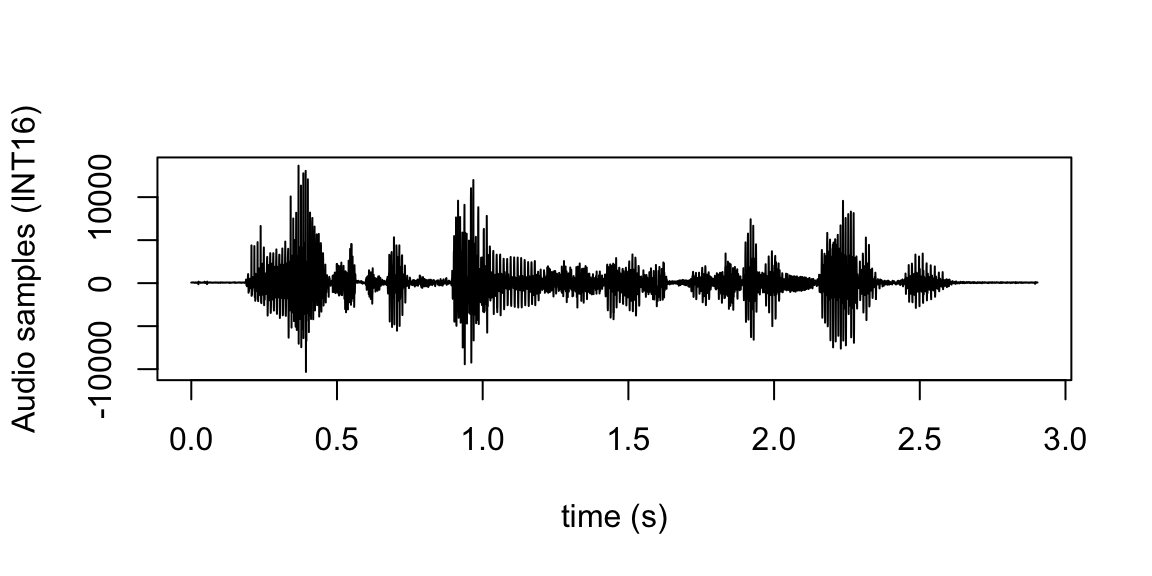
\includegraphics{wrassp_files/figure-latex/wrassp-plotOsci-1.pdf}
\caption{\label{fig:wrassp-plotOsci}Oscillogram generated from samples stored in the \texttt{audio} track of the object \texttt{au}.}
\end{figure}

The export counterpart to \texttt{read.AsspDataObj()} function is \texttt{write.AsspDataObj()}. It is used to store in-memory \texttt{AsspDataObj} objects to disk and is particularly useful for converting other formats to or storing data in the SSFF file format as described in Section \ref{sec:wrassp-genSSFF}. To show how this function can be used to write a slightly altered version of the \texttt{au} object to a file, the R code snippet below initially multiplies all the sample values of \texttt{au\$audio} by a factor of \texttt{0.5}. The resulting \texttt{AsspDataObj} is then written to an audio file in a temporary directory provided by \texttt{R}'s \texttt{tempdir()} function.

\begin{Shaded}
\begin{Highlighting}[]
\CommentTok{# manipulate the audio samples}
\NormalTok{au}\OperatorTok{$}\NormalTok{audio =}\StringTok{ }\NormalTok{au}\OperatorTok{$}\NormalTok{audio }\OperatorTok{*}\StringTok{ }\FloatTok{0.5}
\CommentTok{# write to file in directory}
\CommentTok{# provided by tempdir()}
\KeywordTok{write.AsspDataObj}\NormalTok{(au, }\KeywordTok{file.path}\NormalTok{(}\KeywordTok{tempdir}\NormalTok{(), }\StringTok{'newau.wav'}\NormalTok{))}
\end{Highlighting}
\end{Shaded}

\hypertarget{signal-processing}{%
\section{Signal processing}\label{signal-processing}}

As mentioned in the introduction to this chapter, the \texttt{wrassp} package is capable of more than just the mere importing and exporting of specific signal file formats. This section will focus on demonstrating three of \texttt{wrassp}'s signal processing functions that calculate formant values, their corresponding bandwidths, the fundamental frequency contour and the RMS energy contour. Section \ref{subsec:wrassp-formants} and \ref{subsec:wrassp-f0} demonstrates signal processing to the audio file saved under \texttt{path2wav}, while Section \ref{subsec:wrassp-RMS} adresses processing all the audio files belonging to the \emph{ae} \texttt{emuDB}.

\hypertarget{subsec:wrassp-wrasspOutputInfos}{%
\section{\texorpdfstring{The \texttt{wrasspOutputInfos} object}{The wrasspOutputInfos object}}\label{subsec:wrassp-wrasspOutputInfos}}

The \texttt{wrassp} package comes with the \texttt{wrasspOutputInfos} object, which provides information about the various signal processing functions provided by the package. The \texttt{wrasspOutputInfos} object stores meta information associated with the different signal processing functions \texttt{wrassp} provides. The R code snippet below shows the names of the \texttt{wrasspOutputInfos} object which correspond to the function names listed in the introduction of this chapter.

\begin{Shaded}
\begin{Highlighting}[]
\CommentTok{# show all function names}
\KeywordTok{names}\NormalTok{(wrasspOutputInfos)}
\end{Highlighting}
\end{Shaded}

\begin{verbatim}
##  [1] "acfana"      "afdiff"      "affilter"    "cepstrum"    "cssSpectrum"
##  [6] "dftSpectrum" "ksvF0"       "mhsF0"       "forest"      "lpsSpectrum"
## [11] "rfcana"      "rmsana"      "zcrana"
\end{verbatim}

This object can be useful to get additional information about a specific \texttt{wrassp} function. It contains information about the default file extension (\texttt{\$ext}), the tracks produced (\texttt{\$tracks}) and the output file type (\texttt{\$outputType}). The R code snippet below shows this information for the \texttt{forest()} function.

\begin{Shaded}
\begin{Highlighting}[]
\CommentTok{# show output info of forest function}
\NormalTok{wrasspOutputInfos}\OperatorTok{$}\NormalTok{forest}
\end{Highlighting}
\end{Shaded}

\begin{verbatim}
## $ext
## [1] "fms"
## 
## $tracks
## [1] "fm" "bw"
## 
## $outputType
## [1] "SSFF"
\end{verbatim}

The examples that follow will make use of this \texttt{wrasspOutputInfos} object mainly to acquire the default file extensions given by a specific \texttt{wrassp} signal processing function.

\hypertarget{subsec:wrassp-formants}{%
\section{Formants and their bandwidths}\label{subsec:wrassp-formants}}

The already mentioned \texttt{forest()} is \texttt{wrassp}'s formant estimation function. The default behavior of this formant tracker is to calculate the first four formants and their bandwidths. The R code snippet below shows the usage of this function. As the default behavior of every signal processing function provided by \texttt{wrassp} is to store its result to a file, the \texttt{toFile} parameter of \texttt{forest()} is set to \texttt{FALSE} to prevent this behavior. This results in the same \texttt{AsspDataObj} object as when exporting the result to file and then importing the file into R using \texttt{read.AsspDataObj()}, but circumvents the disk reading/writing overhead.

\begin{Shaded}
\begin{Highlighting}[]
\CommentTok{# calculate formants and corresponding bandwidth values}
\NormalTok{fmBwVals =}\StringTok{ }\KeywordTok{forest}\NormalTok{(path2wav, }\DataTypeTok{toFile =}\NormalTok{ F)}

\CommentTok{# show class vector}
\KeywordTok{class}\NormalTok{(fmBwVals)}
\end{Highlighting}
\end{Shaded}

\begin{verbatim}
## [1] "AsspDataObj"
\end{verbatim}

\begin{Shaded}
\begin{Highlighting}[]
\CommentTok{# show track names}
\KeywordTok{tracks.AsspDataObj}\NormalTok{(fmBwVals)}
\end{Highlighting}
\end{Shaded}

\begin{verbatim}
## [1] "fm" "bw"
\end{verbatim}

\begin{Shaded}
\begin{Highlighting}[]
\CommentTok{# show dimensions of "fm" track}
\KeywordTok{dim}\NormalTok{(fmBwVals}\OperatorTok{$}\NormalTok{fm)}
\end{Highlighting}
\end{Shaded}

\begin{verbatim}
## [1] 581   4
\end{verbatim}

\begin{Shaded}
\begin{Highlighting}[]
\CommentTok{# check dimensions of tracks are the same}
\KeywordTok{all}\NormalTok{(}\KeywordTok{dim}\NormalTok{(fmBwVals}\OperatorTok{$}\NormalTok{fm) }\OperatorTok{==}\StringTok{ }\KeywordTok{dim}\NormalTok{(fmBwVals}\OperatorTok{$}\NormalTok{bw))}
\end{Highlighting}
\end{Shaded}

\begin{verbatim}
## [1] TRUE
\end{verbatim}

As can be seen in the above R code snippet, the object resulting from the \texttt{forest()} function is an object of class \texttt{AsspDataObj} with the tracks \texttt{"fm"} (formants) and \texttt{"bw"} (formant bandwidths), where both track matrices have four columns (corresponding to F1, F2, F3 and F4 in the \texttt{"fm"} track and F1\textsubscript{bandwidth}, F2\textsubscript{bandwidth}, F3\textsubscript{bandwidth} and F4\textsubscript{bandwidth} in the \texttt{"bw"} track) and 581 rows. To visualize the calculated formant values, the R code snippet below shows how R's \texttt{matplot()} function can be used to produce Figure \ref{fig:wrassp-plotFms}.

\begin{Shaded}
\begin{Highlighting}[]
\CommentTok{# plot the formant values}
\KeywordTok{matplot}\NormalTok{(}\KeywordTok{seq}\NormalTok{(}\DecValTok{0}\NormalTok{, }\KeywordTok{numRecs.AsspDataObj}\NormalTok{(fmBwVals) }\OperatorTok{-}\StringTok{ }\DecValTok{1}\NormalTok{)}
        \OperatorTok{/}\StringTok{ }\KeywordTok{rate.AsspDataObj}\NormalTok{(fmBwVals)}
        \OperatorTok{+}\StringTok{ }\KeywordTok{attr}\NormalTok{(fmBwVals, }\StringTok{"startTime"}\NormalTok{),}
\NormalTok{        fmBwVals}\OperatorTok{$}\NormalTok{fm,}
        \DataTypeTok{type =} \StringTok{"l"}\NormalTok{,}
        \DataTypeTok{xlab =} \StringTok{"time (s)"}\NormalTok{,}
        \DataTypeTok{ylab =} \StringTok{"Formant frequency (Hz)"}\NormalTok{)}
\CommentTok{# add legend}
\NormalTok{startFormant =}\StringTok{ }\DecValTok{1}
\NormalTok{endFormant =}\StringTok{ }\DecValTok{4}
\KeywordTok{legend}\NormalTok{(}\StringTok{"topright"}\NormalTok{,}
       \DataTypeTok{legend =} \KeywordTok{paste0}\NormalTok{(}\StringTok{"F"}\NormalTok{, startFormant}\OperatorTok{:}\NormalTok{endFormant),}
       \DataTypeTok{col =}\NormalTok{ startFormant}\OperatorTok{:}\NormalTok{endFormant,}
       \DataTypeTok{lty =}\NormalTok{ startFormant}\OperatorTok{:}\NormalTok{endFormant,}
       \DataTypeTok{bg =} \StringTok{"white"}\NormalTok{)}
\end{Highlighting}
\end{Shaded}

\begin{figure}
\centering
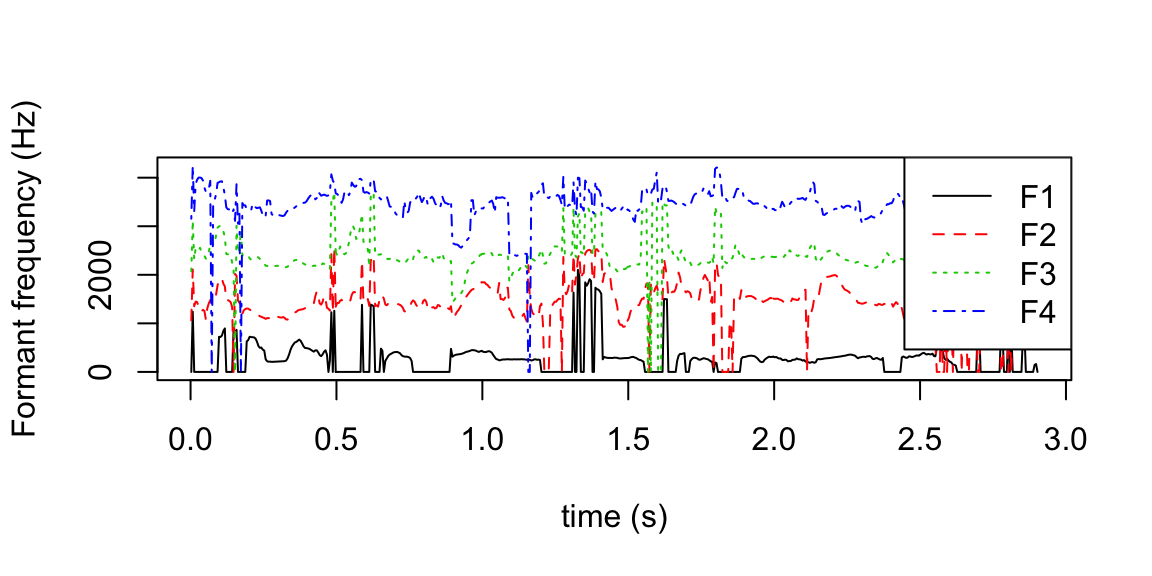
\includegraphics{wrassp_files/figure-latex/wrassp-plotFms-1.pdf}
\caption{\label{fig:wrassp-plotFms}Matrix plot of formant values stored in the \texttt{fm} track of \texttt{fmBwVals} object.}
\end{figure}

\hypertarget{subsec:wrassp_f0}{%
\subsection{Fundamental frequency contour}\label{subsec:wrassp_f0}}

The \texttt{wrassp} package includes two fundamental frequency estimation functions called \texttt{ksvF0()} and \texttt{mhsF0()}. The R code snippet below shows the usage of the \texttt{ksvF0()} function, this time not utilizing the \texttt{toFile} parameter but rather to show an alternative procedure, reading the resulting SSFF file produced by it. It is worth noting that every signal processing function provided by \texttt{wrassp} creates a result file in the same directory as the audio file it was processing (except if the \texttt{outputDirectory} parameter is set otherwise). The default extension given by the \texttt{ksvF0()} is stored in \texttt{wrasspOutputInfos\$ksvF0\$ext}, which is used in the R code snippet below to create the newly generated file's path.

\begin{Shaded}
\begin{Highlighting}[]
\CommentTok{# calculate the fundamental frequency contour}
\KeywordTok{ksvF0}\NormalTok{(path2wav)}

\CommentTok{# create path to newly generated file}
\NormalTok{path2f0file =}\StringTok{ }\KeywordTok{file.path}\NormalTok{(path2bndl,}
                    \KeywordTok{paste0}\NormalTok{(}\StringTok{"msajc003."}\NormalTok{,}
\NormalTok{                           wrasspOutputInfos}\OperatorTok{$}\NormalTok{ksvF0}\OperatorTok{$}\NormalTok{ext))}

\CommentTok{# read file from disk}
\NormalTok{f0vals =}\StringTok{ }\KeywordTok{read.AsspDataObj}\NormalTok{(path2f0file)}
\end{Highlighting}
\end{Shaded}

Analogous to the formant estimation example, the R code snippet below shows how the \texttt{plot()} function can be used to visualize this data as in Figure \ref{fig:wrassp-plotF0}.

\begin{Shaded}
\begin{Highlighting}[]
\CommentTok{# plot the fundamental frequency contour}
\KeywordTok{plot}\NormalTok{(}\KeywordTok{seq}\NormalTok{(}\DecValTok{0}\NormalTok{,}\KeywordTok{numRecs.AsspDataObj}\NormalTok{(f0vals) }\OperatorTok{-}\StringTok{ }\DecValTok{1}\NormalTok{)}
     \OperatorTok{/}\StringTok{ }\KeywordTok{rate.AsspDataObj}\NormalTok{(f0vals) }\OperatorTok{+}
\StringTok{       }\KeywordTok{attr}\NormalTok{(f0vals, }\StringTok{"startTime"}\NormalTok{),}
\NormalTok{     f0vals}\OperatorTok{$}\NormalTok{F0,}
     \DataTypeTok{type =} \StringTok{"l"}\NormalTok{,}
     \DataTypeTok{xlab =} \StringTok{"time (s)"}\NormalTok{,}
     \DataTypeTok{ylab =} \StringTok{"F0 frequency (Hz)"}\NormalTok{)}
\end{Highlighting}
\end{Shaded}

\begin{figure}
\centering
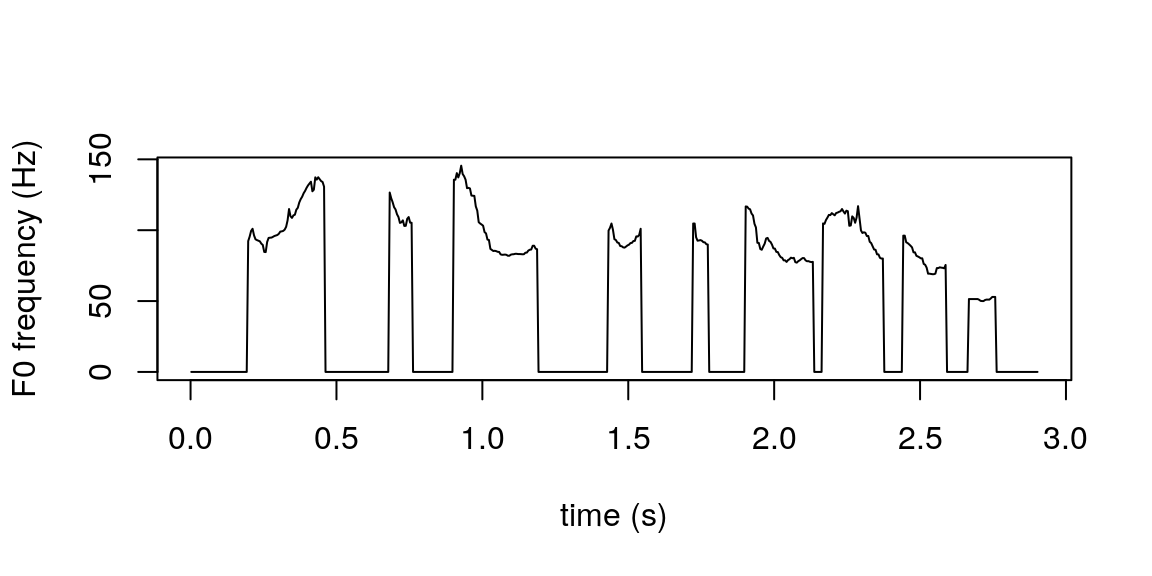
\includegraphics{wrassp_files/figure-latex/wrassp-plotF0-1.pdf}
\caption{\label{fig:wrassp-plotF0}Plot of fundamental frequency values stored in the \texttt{F0} track of \texttt{f0vals} object.}
\end{figure}

\hypertarget{subsec:wrassp-RMS}{%
\subsection{RMS energy contour}\label{subsec:wrassp-RMS}}

The \texttt{wrassp} function for calculating the short-term root mean square (RMS) amplitude of the signal is called \texttt{rmsana()}. As its usage is analogous to the above examples, here we will focus on using it to calculate the RMS values for all the audio files of the \texttt{ae} \texttt{emuDB}. The R code snippet below initially uses the \texttt{list\_files()} function to aquire the file paths for every \texttt{.wav} file in the \texttt{ae} \texttt{emuDB}. As every signal processing function accepts one or multiple file paths, these file paths can simply be passed in as the main argument to the \texttt{rmsana()} function. As all of \texttt{wrassp}'s signal processing functions place their generated files in the same directory as the audio file they process, the \texttt{rmsana()} function will automatically place every \texttt{.rms} into the correct bundle directory.

\begin{Shaded}
\begin{Highlighting}[]
\CommentTok{# list all .wav files in the ae emuDB}
\NormalTok{paths2wavFiles =}\StringTok{ }\KeywordTok{list_files}\NormalTok{(ae, }\DataTypeTok{fileExtension =} \StringTok{"wav"}\NormalTok{)}\OperatorTok{$}\NormalTok{absolute_file_path}

\CommentTok{# calculate the RMS energy values for all .wav files}
\KeywordTok{rmsana}\NormalTok{(paths2wavFiles)}

\CommentTok{# list new .rms files using}
\CommentTok{# wrasspOutputInfos->rmsana->ext}
\NormalTok{rmsFPs =}\StringTok{ }\KeywordTok{list.files}\NormalTok{(path2ae,}
                    \DataTypeTok{pattern =} \KeywordTok{paste0}\NormalTok{(}\StringTok{".*"}\NormalTok{,}
\NormalTok{                                     wrasspOutputInfos}\OperatorTok{$}\NormalTok{rmsana}\OperatorTok{$}\NormalTok{ext),}
                    \DataTypeTok{recursive =} \OtherTok{TRUE}\NormalTok{,}
                    \DataTypeTok{full.names =} \OtherTok{TRUE}\NormalTok{)}

\CommentTok{# read first RMS file}
\NormalTok{rmsvals =}\StringTok{ }\KeywordTok{read.AsspDataObj}\NormalTok{(rmsFPs[}\DecValTok{1}\NormalTok{])}
\end{Highlighting}
\end{Shaded}

The R code snippet below shows how the \texttt{plot()} function can be used to visualize this data as in Figure \ref{fig:wrassp-plotRMS}.

\begin{Shaded}
\begin{Highlighting}[]
\CommentTok{# plot the RMS energy contour}
\KeywordTok{plot}\NormalTok{(}\KeywordTok{seq}\NormalTok{(}\DecValTok{0}\NormalTok{, }\KeywordTok{numRecs.AsspDataObj}\NormalTok{(rmsvals) }\OperatorTok{-}\StringTok{ }\DecValTok{1}\NormalTok{)}
     \OperatorTok{/}\StringTok{ }\KeywordTok{rate.AsspDataObj}\NormalTok{(rmsvals)}
     \OperatorTok{+}\StringTok{ }\KeywordTok{attr}\NormalTok{(rmsvals, }\StringTok{"startTime"}\NormalTok{),}
\NormalTok{     rmsvals}\OperatorTok{$}\NormalTok{rms,}
     \DataTypeTok{type =} \StringTok{"l"}\NormalTok{,}
     \DataTypeTok{xlab =} \StringTok{"time (s)"}\NormalTok{,}
     \DataTypeTok{ylab =} \StringTok{"RMS energy (dB)"}\NormalTok{)}
\end{Highlighting}
\end{Shaded}

\begin{figure}
\centering
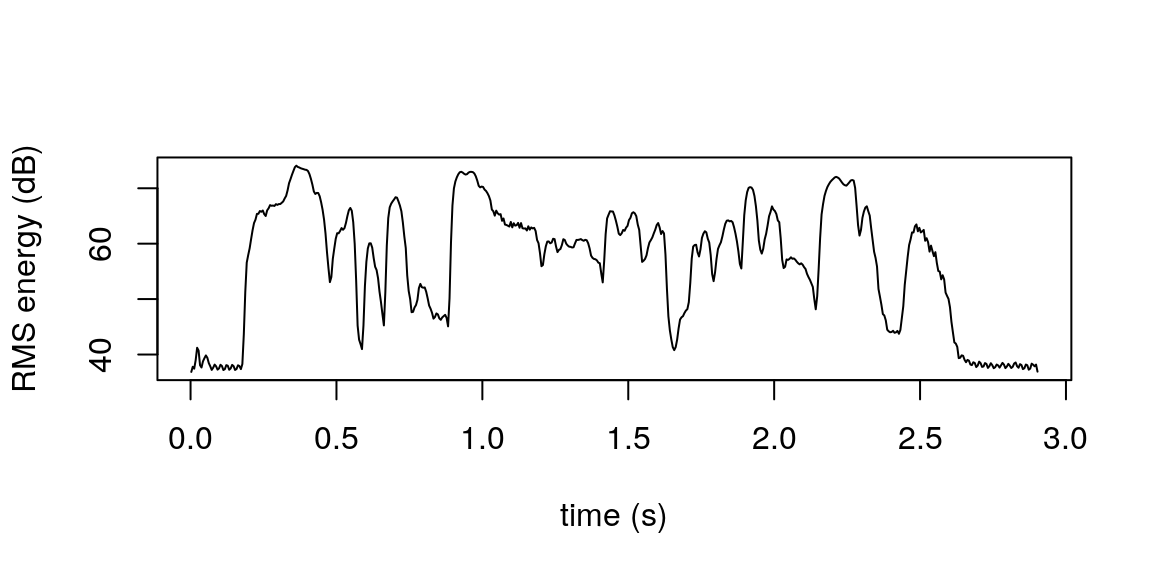
\includegraphics{wrassp_files/figure-latex/wrassp-plotRMS-1.pdf}
\caption{\label{fig:wrassp-plotRMS}Plot of RMS values stored in \texttt{rms} track of the \texttt{rmsvals} object.}
\end{figure}

\hypertarget{sec:wrassp_logging}{%
\section{\texorpdfstring{Logging \texttt{wrassp}'s function calls}{Logging wrassp's function calls}}\label{sec:wrassp_logging}}

As it can be extremely important to keep track of information about how certain files are created and calculated, every signal processing function provided by the \texttt{wrassp} package comes with the ability to log its function calls to a specified log file. The R code snippet below shows a call to the \texttt{ksvF0()} function where a single parameter was changed from its default value (\texttt{windowShift\ =\ 10}). The content of the created log files (shown by the call to \texttt{readLines()}) contains the function name, time stamp, parameters that were altered and processed file path information. It is worth noting that a log file can be reused for multiple function calls as the log function does not overwrite an existing file but merely appends new log information to it.

\begin{Shaded}
\begin{Highlighting}[]
\CommentTok{# create path to log file in root dir of ae emuDB}
\NormalTok{path2logFile =}\StringTok{ }\KeywordTok{file.path}\NormalTok{(path2ae, }\StringTok{"wrassp.log"}\NormalTok{)}

\CommentTok{# calculate the fundamental frequency contour}
\KeywordTok{ksvF0}\NormalTok{(path2wav, }
      \DataTypeTok{windowShift =} \DecValTok{10}\NormalTok{,}
      \DataTypeTok{forceToLog =}\NormalTok{ T, }
      \DataTypeTok{optLogFilePath =}\NormalTok{ path2logFile)}
\end{Highlighting}
\end{Shaded}

\begin{verbatim}
## [1] 1
\end{verbatim}

\begin{Shaded}
\begin{Highlighting}[]
\CommentTok{# display content of log file (first 8 lines)}
\KeywordTok{readLines}\NormalTok{(path2logFile)[}\DecValTok{1}\OperatorTok{:}\DecValTok{8}\NormalTok{]}
\end{Highlighting}
\end{Shaded}

\begin{verbatim}
## [1] ""                                   "##################################"
## [3] "##################################" "######## ksvF0 performed ########" 
## [5] "Timestamp:  2020-02-06 12:05:05 "   "windowShift : 10 "                 
## [7] "forceToLog : T "                    " => on files:"
\end{verbatim}

\hypertarget{sec:wrassp-emu-sdms}{%
\section{\texorpdfstring{Using \texttt{wrassp} in the EMU-SDMS}{Using wrassp in the EMU-SDMS}}\label{sec:wrassp-emu-sdms}}

As shown in Section \ref{subsec:wrassp-RMS}, the \texttt{wrassp} signal processing functions can be used to calculate SSFF files and place them into the appropriate bundle directories. The only thing that has to be done to make an \texttt{emuDB} aware of these files is to add an SSFF track definition to the \texttt{emuDB} as shown in the R code snippet below. Once added, this SSFF track can be referenced via the \texttt{ssffTrackName} parameter of the \texttt{get\_trackdata()} function as shown in various examples throughout this documentation. It is worth noting that this strategy is not necessarily relevant for applying the same signal processing to an entire \texttt{emuDB}, as this can be achieved using the on-the-fly \texttt{add\_ssffTrackDefinition()} method described in the according R code snippet below. However, it becomes necessary if certain bundles are to be processed using deviating function parameters. This can, for example, be relevant when setting the minimum and maximum frequencies that are to be considered while estimating the fundamental frequencies (e.g., the \texttt{maxF} and \texttt{minF} of \texttt{ksvfF0()}) for female versus male speakers.

\begin{Shaded}
\begin{Highlighting}[]
\CommentTok{# load emuDB}
\NormalTok{ae =}\StringTok{ }\KeywordTok{load_emuDB}\NormalTok{(path2ae)}

\CommentTok{# add SSFF track defintion}
\CommentTok{# that references the .rms files}
\CommentTok{# calculated above}
\CommentTok{# (i.e. no new files are calculated and added to the emuDB)}
\NormalTok{ext =}\StringTok{ }\NormalTok{wrasspOutputInfos}\OperatorTok{$}\NormalTok{rmsana}\OperatorTok{$}\NormalTok{ext}
\NormalTok{colName =}\StringTok{ }\NormalTok{wrasspOutputInfos}\OperatorTok{$}\NormalTok{rmsana}\OperatorTok{$}\NormalTok{tracks[}\DecValTok{1}\NormalTok{]}
\KeywordTok{add_ssffTrackDefinition}\NormalTok{(ae,}
                        \DataTypeTok{name =} \StringTok{"rms"}\NormalTok{,}
                        \DataTypeTok{fileExtension =}\NormalTok{ ext,}
                        \DataTypeTok{columnName =}\NormalTok{ colName)}
\end{Highlighting}
\end{Shaded}

A further way to utilize \texttt{wrassp}'s signal processing functions as part of the EMU-SDMS is via the \texttt{onTheFlyFunctionName} and \texttt{onTheFlyParams} parameters of the \texttt{add\_ssffTrackDefinition()} and \texttt{get\_trackdata()} functions. Using the \texttt{onTheFlyFunctionName} parameter in the \texttt{add\_ssffTrackDefinition()} function automatically calculates the SSFF files while also adding the SSFF track definition. Using this parameter with the \texttt{get\_trackdata()} function calls the given \texttt{wrassp} function with the \texttt{toFile} parameter set to \texttt{FALSE} and extracts the matching segments and places them in the resulting \texttt{trackdata} or \texttt{emuRtrackdata} object. In many cases, this avoids the necessity of having SSFF track definitions in the \texttt{emuDB}. In both functions, the optional \texttt{onTheFlyParams} parameter can be used to specify the parameters that are passed into the signal processing function. The R code snippet below shows how R's \texttt{formals()} function can be used to get all the parameters of \texttt{wrassp}'s short-term positive and negative zero-crossing rate (ZCR) analysis function \texttt{zrcana()}. It then changes the default window size parameter to a new value and passes the parameters object into the \texttt{add\_ssffTrackDefinition()} and \texttt{get\_trackdata()} functions.

\begin{Shaded}
\begin{Highlighting}[]
\CommentTok{# get all parameters of zcrana}
\NormalTok{zcranaParams =}\StringTok{ }\KeywordTok{formals}\NormalTok{(}\StringTok{"zcrana"}\NormalTok{)}

\CommentTok{# show names of parameters}
\KeywordTok{names}\NormalTok{(zcranaParams)}
\end{Highlighting}
\end{Shaded}

\begin{verbatim}
##  [1] "listOfFiles"     "optLogFilePath"  "beginTime"       "centerTime"     
##  [5] "endTime"         "windowShift"     "windowSize"      "toFile"         
##  [9] "explicitExt"     "outputDirectory" "forceToLog"      "verbose"
\end{verbatim}

\begin{Shaded}
\begin{Highlighting}[]
\CommentTok{# change window size from the default}
\CommentTok{# value of 25 ms to 50 ms}
\NormalTok{zcranaParams}\OperatorTok{$}\NormalTok{windowSize =}\StringTok{ }\DecValTok{50}

\CommentTok{# to have a segment list to work with}
\CommentTok{# query all Phonetic 'n' segments}
\NormalTok{sl =}\StringTok{ }\KeywordTok{query}\NormalTok{(ae, }\StringTok{"Phonetic == n"}\NormalTok{)}

\CommentTok{# get trackdata calculating ZCR values on-the-fly}
\CommentTok{# using the above parameters. Note that no files}
\CommentTok{# are generated.}
\CommentTok{# (verbose = F is only set to avoid additional output in manual)}
\NormalTok{td =}\StringTok{ }\KeywordTok{get_trackdata}\NormalTok{(ae, sl,}
                   \DataTypeTok{onTheFlyFunctionName =} \StringTok{"zcrana"}\NormalTok{,}
                   \DataTypeTok{onTheFlyParams =}\NormalTok{ zcranaParams,}
                   \DataTypeTok{verbose =} \OtherTok{FALSE}\NormalTok{)}


\CommentTok{# add SSFF track definition. Note that}
\CommentTok{# this time files are generated.}
\CommentTok{# (verbose = F is only set to avoid additional output in manual)}
\KeywordTok{add_ssffTrackDefinition}\NormalTok{(ae,}
                        \DataTypeTok{name =} \StringTok{"zcr"}\NormalTok{,}
                        \DataTypeTok{onTheFlyFunctionName =} \StringTok{"zcrana"}\NormalTok{,}
                        \DataTypeTok{onTheFlyParams =}\NormalTok{ zcranaParams,}
                        \DataTypeTok{verbose =} \OtherTok{FALSE}\NormalTok{)}
\end{Highlighting}
\end{Shaded}

\hypertarget{sec:wrassp_genSSFF}{%
\section{Storing data in the SSFF file format}\label{sec:wrassp_genSSFF}}

One of the benefits gained by having the \texttt{AsspDataObj} in-memory object is that these objects can be constructed from scratch in R, as they are basically simple \texttt{list} objects. This means, for example, that any set of n-dimensional samples over time can be placed in a \texttt{AsspDataObj} and then stored as an SSFF file using the \texttt{write.AsspDataObj()} function. To show how this can be done, the R code snippet below creates an arbitrary data sample in the form of a single cycle sine wave between \(0\) and \(2*pi\) that is made up of 16000 samples and displays it in Figure \ref{fig:wrassp-genSin}.

\begin{Shaded}
\begin{Highlighting}[]
\NormalTok{x =}\StringTok{ }\KeywordTok{seq}\NormalTok{(}\DecValTok{0}\NormalTok{, }\DecValTok{2} \OperatorTok{*}\StringTok{ }\NormalTok{pi, }\DataTypeTok{length.out =} \DecValTok{16000}\NormalTok{)}
\NormalTok{sineWave =}\StringTok{ }\KeywordTok{sin}\NormalTok{(x)}
\KeywordTok{plot}\NormalTok{(x, sineWave, }\DataTypeTok{type =} \StringTok{'l'}\NormalTok{,}
     \DataTypeTok{xlab =} \StringTok{"x from 0 to 2*pi"}\NormalTok{,}
     \DataTypeTok{ylab =} \StringTok{""}\NormalTok{)}
\end{Highlighting}
\end{Shaded}

\begin{figure}
\centering
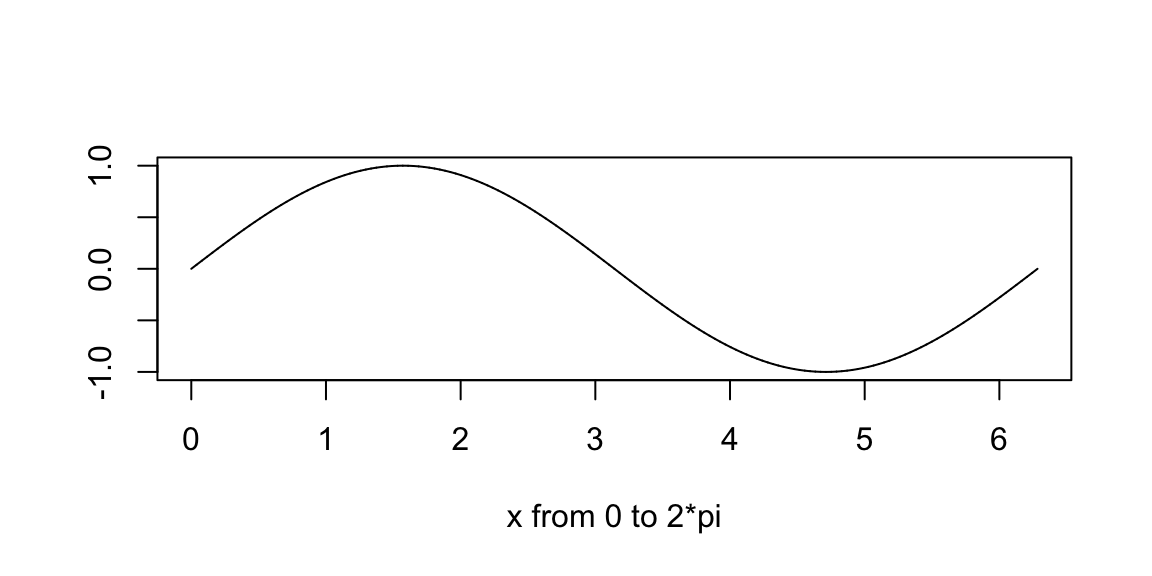
\includegraphics{wrassp_files/figure-latex/wrassp-genSin-1.pdf}
\caption{\label{fig:wrassp-genSin}A single cycle sine wave consisting of 16000 samples.}
\end{figure}

Assuming a sample rate of 16 kHz \texttt{sineWave} would result in a sine wave with a frequency of 1 Hz and a duration of one second. The R code snippet below shows how a \texttt{AsspDataObj} can be created from scratch and the data in \texttt{sineWave} placed into one of its tracks. It then goes on to write the \texttt{AsspDataObj} object to an SSFF file.

\begin{Shaded}
\begin{Highlighting}[]
\CommentTok{# create empty list object}
\NormalTok{ado =}\StringTok{ }\KeywordTok{list}\NormalTok{()}

\CommentTok{# add sample rate attribute}
\KeywordTok{attr}\NormalTok{(ado, }\StringTok{"sampleRate"}\NormalTok{) =}\StringTok{ }\DecValTok{16000}

\CommentTok{# add start time attribute}
\KeywordTok{attr}\NormalTok{(ado, }\StringTok{"startTime"}\NormalTok{) =}\StringTok{ }\DecValTok{0}

\CommentTok{# add start record attribute}
\KeywordTok{attr}\NormalTok{(ado, }\StringTok{"startRecord"}\NormalTok{) =}\StringTok{ }\KeywordTok{as.integer}\NormalTok{(}\DecValTok{1}\NormalTok{)}

\CommentTok{# add end record attribute}
\KeywordTok{attr}\NormalTok{(ado, }\StringTok{"endRecord"}\NormalTok{) =}\StringTok{ }\KeywordTok{as.integer}\NormalTok{(}\KeywordTok{length}\NormalTok{(sineWave))}

\CommentTok{# set class of ado}
\KeywordTok{class}\NormalTok{(ado) =}\StringTok{ "AsspDataObj"}

\CommentTok{# show available file formats}
\NormalTok{AsspFileFormats}
\end{Highlighting}
\end{Shaded}

\begin{verbatim}
##     RAW   ASP_A   ASP_B   XASSP  IPDS_M  IPDS_S    AIFF    AIFC     CSL    CSRE 
##       1       2       3       4       5       6       7       8       9      10 
##    ESPS     ILS     KTH   SWELL   SNACK     SFS     SND      AU    NIST  SPHERE 
##      11      12      13      13      13      14      15      15      16      16 
## PRAAT_S PRAAT_L PRAAT_B    SSFF    WAVE  WAVE_X  XLABEL    YORK     UWM 
##      17      18      19      20      21      22      24      25      26
\end{verbatim}

\begin{Shaded}
\begin{Highlighting}[]
\CommentTok{# set file format to SSFF}
\CommentTok{# }\AlertTok{NOTE}\CommentTok{: assignment of "SSFF" also possible}
\KeywordTok{AsspFileFormat}\NormalTok{(ado) =}\StringTok{ }\KeywordTok{as.integer}\NormalTok{(}\DecValTok{20}\NormalTok{)}

\CommentTok{# set data format (1 == 'ascii' and 2 == 'binary')}
\KeywordTok{AsspDataFormat}\NormalTok{(ado) =}\StringTok{ }\KeywordTok{as.integer}\NormalTok{(}\DecValTok{2}\NormalTok{)}

\CommentTok{# set track format specifiers}
\CommentTok{# (available track formats for numbers}
\CommentTok{# that match their C equivalent are:}
\CommentTok{# "UINT8"; "INT8"; "UINT16"; "INT16";}
\CommentTok{# "UINT24"; "INT24"; "UINT32"; "INT32";}
\CommentTok{# "UINT64"; "INT64"; "REAL32"; "REAL64");}
\KeywordTok{attr}\NormalTok{(ado, }\StringTok{"trackFormats"}\NormalTok{) =}\StringTok{ }\KeywordTok{c}\NormalTok{(}\StringTok{"REAL32"}\NormalTok{)}

\CommentTok{# add track}
\NormalTok{ado =}\StringTok{ }\KeywordTok{addTrack}\NormalTok{(ado, }\StringTok{"sine"}\NormalTok{, sineWave, }\StringTok{"REAL32"}\NormalTok{)}

\CommentTok{# write AsspDataObj object to file}
\KeywordTok{write.AsspDataObj}\NormalTok{(}\DataTypeTok{dobj =}\NormalTok{ ado,}
                  \DataTypeTok{file =} \KeywordTok{file.path}\NormalTok{(}\KeywordTok{tempdir}\NormalTok{(), }\StringTok{"example.sine"}\NormalTok{))}
\end{Highlighting}
\end{Shaded}

\begin{verbatim}
## NULL
\end{verbatim}

Although somewhat of a generic example, the above R code snippet shows how to generate an \texttt{AsspDataObj} from scratch. This approach can, for example, be used to read in signal data produced by other software or signal data acquisition devices. Hence, this approach can be used to import many forms of data into the EMU-SDMS. Appendix \ref{sec:app-chap-wrassp-praatsSigProc} shows an example of how this approach can be used to take advantage of Praat's signal processing capabilities and integrate its output into the EMU-SDMS.

\hypertarget{conclusion-4}{%
\section{Conclusion}\label{conclusion-4}}

The \texttt{wrassp} packages enriches the R package landscape by providing functionality for handling speech signal files in most common audio formats and for performing signal analyses common in the phonetic and speech sciences. The EMU-SDMS utilizes the functionality that the \texttt{wrassp} package provides by allowing the user to calculate signals that match the segments of a segment list. This can either be done in real time or by extracting the signals from files. Hence, the \texttt{wrassp} package is an integral part of the EMU-SDMS but can also be used as a standalone package if so desired.

\hypertarget{chap:emu-webApp}{%
\chapter[The \texttt{EMU-webApp} ]{\texorpdfstring{The \texttt{EMU-webApp} \footnote{Sections of this chapter have been published in \citep{winkelmann:2015d} and some descriptions where taken from the \texttt{EMU-webApp}'s own manual.}}{The EMU-webApp }}\label{chap:emu-webApp}}

\begin{center}\includegraphics[width=0.75\linewidth]{pics/EMU-webAppEmu_emu-webApp} \end{center}

The EMU-SDMS has a unique approach to its graphical user interface (GUI) in that it utilizes a web application as its primary GUI. This is known as the \texttt{EMU-webApp} \citep{winkelmann:2015d}. The \texttt{EMU-webApp} is a fully fledged browser-based labeling and correction tool that offers a multitude of labeling and visualization features. These features include unlimited undo/redo, formant correction capabilities, the ability to snap a preselected boundary to the nearest top/bottom boundary, snap a preselected boundary to the nearest zero crossing, and many more. The web application is able to render everything directly in the user's browser, including the calculation and rendering of the spectrogram, as it is written entirely using HTML, CSS and JavaScript. This means it can also be used as a standalone labeling application, as it does not require any server-side calculations or rendering. Further, it is designed to interact with any websocket server that implements the \texttt{EMU-webApp} websocket protocol (see Section \ref{subsec:emu-webAppTheProtocol}). This enables it to be used as a labeling tool for collaborative annotation efforts. Also, as the \texttt{EMU-webApp} is cached in the user's browser on the first visit, it does not require any internet connectivity to be able to access the web application unless the user explicitly clears the browser's cache. The URL of the current live version of the \texttt{EMU-webApp} is: \url{http://ips-lmu.github.io/EMU-webApp/}.

\hypertarget{sec:emu-webApp-mainLayout}{%
\section{Main layout}\label{sec:emu-webApp-mainLayout}}

The main screen of the \texttt{EMU-webApp} can be split into five areas. Figure \ref{fig:emu-web-emuWebAppLayout} shows a screenshot of the \texttt{EMU-webApp}'s main screen displaying these five areas while displaying a bundle of the \emph{ae} demo database. This database is served to the \texttt{EMU-webApp} by invoking the \texttt{serve()} command as shown in the R code snippet below. The left side bar (area marked 1 in Figure \ref{fig:emu-web-emuWebAppLayout}) represents the bundle list side bar which, if connected to a database, displays the currently available bundles grouped by their sessions. The top and bottom menu bars (areas marked 2 and 5 in Figure \ref{fig:emu-web-emuWebAppLayout}) display the currently available menu options, where the bottom menu bar contains the audio navigation and playback controls and also includes a scrollable mini map of the oscillogram. Area 3 of Figure \ref{fig:emu-web-emuWebAppLayout} displays the signal canvas area currently displaying the oscillogram and the spectrogram. Other signal contours such as formant frequency contours and fundamental frequency contours are also displayed in this area. Area 4 of Figure \ref{fig:emu-web-emuWebAppLayout} displays the area in which levels containing time information are displayed. It is worth noting that the main screen of the \texttt{EMU-webApp} does not display any levels that do not contain time information. The hierarchical annotation can be displayed and edited by clicking the \texttt{show\ hierarchy} button in the top menu bar (see Figure \ref{fig:webApp-hierModal} for an example of how the hierarchy is displayed).

\begin{Shaded}
\begin{Highlighting}[]
\CommentTok{# serve ae emuDB to EMU-webApp}
\KeywordTok{serve}\NormalTok{(ae)}
\end{Highlighting}
\end{Shaded}

\begin{figure}

{\centering \includegraphics[width=1\linewidth]{pics/emu-webAppLayout} 

}

\caption{Screenshot of `EMU-webApp` displaying the *ae* demo database with overlaid areas of the main screen of the web application (see text).}\label{fig:emu-web-emuWebAppLayout}
\end{figure}

\hypertarget{sec:webApp-generalUsage}{%
\section{General usage}\label{sec:webApp-generalUsage}}

This section introduces the labeling mechanics and general labeling workflow of the \texttt{EMU-webApp}. The \texttt{EMU-webApp} makes heavy use of keyboard shortcuts. Is is worth noting that most of the keyboard shortcuts are centered around the \texttt{WASD} keys, which are the navigation shortcut keys (\texttt{W} to zoom in; \texttt{S} to zoom out; \texttt{A} to move left and \texttt{D} to move right). For a full list of the available keyboard shortcuts see the \texttt{EMU-webApp}'s own manual, which can be accessed by clicking the EMU icon on the right hand side of the top menu bar (area 2 in Figure \ref{fig:emu-web-emuWebAppLayout}).

\hypertarget{annotating-levels-containing-time-information}{%
\subsection{Annotating levels containing time information}\label{annotating-levels-containing-time-information}}

\hypertarget{boundaries-and-events}{%
\subsubsection*{Boundaries and events}\label{boundaries-and-events}}
\addcontentsline{toc}{subsubsection}{Boundaries and events}

The \texttt{EMU-webApp} has slightly different labeling mechanics compared with other annotation software. Compared to the usual click and drag of segment boundaries and event markers, the web application continuously tracks the movement of the mouse in levels containing time information, highlighting the boundary or event marker that is closest to it by coloring it blue. Figure \ref{fig:webApp-preSelBoundary} displays this automatic boundary preselection.

\begin{figure}

{\centering \includegraphics[width=0.4\linewidth]{pics/preSelBoundary} 

}

\caption{Screenshot of segment level as displayed by the `EMU-webApp` with superimposed mouse cursor displaying the automatic boundary preselection of closest boundary (boundary marked blue).}\label{fig:webApp-preSelBoundary}
\end{figure}

Once a boundary or event is preselected, the user can perform various actions with it. She or he can, for example, grab a preselected boundary or event by holding down the \texttt{SHIFT} key and moving it to the desired position, or delete the current boundary or event by hitting the \texttt{BACKSPACE} key. Other actions that can be performed on preselected boundaries or events are:

\begin{itemize}
\tightlist
\item
  snap to closest boundary or event in level above (Keyboard Shortcut \texttt{t}),
\item
  snap to closest boundary or event in level below (Keyboard Shortcut \texttt{b}), and
\item
  snap to nearest zero crossing (Keyboard Shortcut \texttt{x}).
\end{itemize}

To add a new boundary or event to a level the user initially has to select the desired level she or he wishes to edit. This is achieved either by using the up and down cursor keys or by single-left-clicking on the desired level. The current preselected level is marked in a darker shade of gray, as is displayed in Figure \ref{fig:webApp-selectLevel}.

\begin{figure}

{\centering \includegraphics[width=0.4\linewidth]{pics/selectLevel} 

}

\caption{Screenshot of two levels as displayed by the `EMU-webApp`, where the lower level is preselected (i.e., marked in a darker shade of gray).}\label{fig:webApp-selectLevel}
\end{figure}

To add a boundary to the currently selected level one first has to select a point in time either in the spectrogram or the oscillogram by single-left-clicking on the desired location. Hitting the enter/return key adds a new boundary or event to the preselected level at the selected time point. Selecting a stretch of time in the spectrogram or the oscillogram (left-click-and-drag) and hitting enter will add a segment (not a boundary) to a preselected segment level.

\hypertarget{segments-events}{%
\subsubsection*{Segments and events}\label{segments-events}}
\addcontentsline{toc}{subsubsection}{Segments and events}

The \texttt{EMU-webApp} also allows segments and events to be preselected by single-left-clicking the desired item. The web application colors the preselected segments and events yellow to indicate their pre-selection as displayed in Figure \ref{fig:webApp-preSelSeg}.

\begin{figure}

{\centering \includegraphics[width=0.4\linewidth]{pics/preSelSeg} 

}

\caption{Screenshot of level as displayed by the `EMU-webApp`, where the /@/ segment is currently preselected as it is marked yellow.}\label{fig:webApp-preSelSeg}
\end{figure}

As with preselected boundaries or events the user can now perform multiple actions with these preselected items. She or he can, for example, edit the item's label by hitting the enter/return key (which can also be achieved by double-left-clicking the item). Other actions that can be performed on preselected items are:

\begin{itemize}
\tightlist
\item
  Select next item in level (keyboard shortcut \texttt{TAB}),
\item
  Select previous item in level (keyboard shortcut \texttt{SHIFT} plus \texttt{TAB}),
\item
  Add time to selected item(s) end (keyboard shortcut \texttt{+}),
\item
  Add time to selected item(s) start (keyboard shortcut \texttt{SHIFT} plus \texttt{+}),
\item
  Remove time to selected item(s) end (keyboard shortcut \texttt{-}),
\item
  Remove time to selected item(s) start (keyboard shortcut \texttt{SHIFT} plus \texttt{-}), and
\item
  Move selected item(s) (hold down \texttt{ALT} Key and drag to desired position).
\end{itemize}

By right-clicking adjacent segment or events (keyboard shortcut \texttt{SHIFT} plus left or right cursor keys), it is possible to select multiple items at once.

\hypertarget{parallel-labels-in-segments-and-events}{%
\subsubsection*{Parallel labels in segments and events}\label{parallel-labels-in-segments-and-events}}
\addcontentsline{toc}{subsubsection}{Parallel labels in segments and events}

If a level containing time information has multiple attribute definitions (i.e., multiple parallel labels per segment or event) the \texttt{EMU-webApp} automatically displays radio buttons underneath that level (see red square in Figure \ref{fig:webApp-parTimeLevel}) that allow the user to switch between the parallel labels. Figure \ref{fig:webApp-parTimeLevel} displays a segment level with three attribute definitions.

\begin{figure}

{\centering \includegraphics[width=0.75\linewidth]{pics/emu-webAppParTimeLevel} 

}

\caption{Screenshot of segment level with three attribute definitions. The radio buttons that switch between the parallel labels are highlighted by a red square.}\label{fig:webApp-parTimeLevel}
\end{figure}

\hypertarget{legal-labels}{%
\subsubsection*{Legal labels}\label{legal-labels}}
\addcontentsline{toc}{subsubsection}{Legal labels}

As mentioned in Section \ref{subsubsec:emuDBlegalLabels}, an array of so-called legal labels can be defined for every level or, more specifically, for each attribute definition. The \texttt{EMU-webApp} enforces these legal labels by not allowing any other labels to be entered in the label editing text fields. If an illegal label is entered, the text field will turn red and the \texttt{EMU-webApp} will not permit this label to be saved.

\hypertarget{working-with-hierarchical-annotations-2-chapemu-webapp}{%
\subsection[Working with hierarchical annotations ]{\texorpdfstring{Working with hierarchical annotations \footnote{This section is an updated version of the \emph{The level hierarchy} section of the \emph{General Usage} chapter that is part of the \texttt{EMU-webApp} own brief manual by Markus Jochim.}}{Working with hierarchical annotations }}\label{working-with-hierarchical-annotations-2-chapemu-webapp}}

\hypertarget{viewing-the-hierarchy}{%
\subsubsection*{Viewing the hierarchy}\label{viewing-the-hierarchy}}
\addcontentsline{toc}{subsubsection}{Viewing the hierarchy}

As mentioned in Section \ref{sec:emu-webApp-mainLayout}, pressing the \texttt{show\ hierarchy} button (keyboard shortcut \texttt{h}) in the top menu bar opens the hierarchy view modal window\footnote{The term modal window is used in user interface design to refer to pop-up windows that force the user to interact with the window before returning back to the main application.}. As with most modal windows in the \texttt{EMU-webApp}, it can be closed by clicking on the \texttt{close} button, clicking the X circle icon in the top right hand corner of the modal or by hitting the \texttt{ESCAPE} key. By default, the hierarchy modal window displays a horizontal version of the hierarchy for a spatially economical visualization. As most people are more familiar with a vertical hierarchical annotation display, the hierarchy can be rotated by hitting the \texttt{rotate\ by\ 90°} button (keyboard shortcut \texttt{r}). Zooming in and out of the hierarchy can be achieved by using the mouse wheel, and moving through the hierarchy in time can be achieved by holding down the left mouse button and dragging the hierarchy in the desired direction. Figure \ref{fig:webApp-hierModal} shows the hierarchy modal window displaying the hierarchical annotation of a single path (\emph{Utterance} -\textgreater{} \emph{Intonational} -\textgreater{} \emph{Intermediate} -\textgreater{} \emph{Word} -\textgreater{} \emph{Syllable} -\textgreater{} \emph{Phoneme} -\textgreater{} \emph{Phonetic}) through a multi-path hierarchy of the \emph{ae} \texttt{emuDB} in its horizontal form.

\begin{figure}

{\centering \includegraphics[width=0.75\linewidth]{pics/emu-webAppHierModal} 

}

\caption{Screenshot of the hierarchy modal window level displaying a path through the hierarchy of the *ae* `emuDB` in its horizontal form.}\label{fig:webApp-hierModal}
\end{figure}

\hypertarget{selecting-a-path-through-the-hierarchy}{%
\subsubsection*{Selecting a path through the hierarchy}\label{selecting-a-path-through-the-hierarchy}}
\addcontentsline{toc}{subsubsection}{Selecting a path through the hierarchy}

As more complex databases have multiple hierarchical paths through their hierarchical annotation structure (see Figure \ref{fig:annotStruct}B for an example of a multi-dimensional hierarchical annotation structure), the hierarchy modal offers a drop-down menu to choose the current path to be displayed. Area 2 in Figure \ref{fig:webApp-hierModalTop} marks the hierarchy path drop-down menu of the hierarchy modal.

\begin{figure}

{\centering \includegraphics[width=0.85\linewidth]{pics/emu-webAppHierModalTop} 

}

\caption{Screenshot of top of hierarchy modal window of the `EMU-webApp` in which the area marked 1 shows the drop-down menus for selecting the parallel label for each level and area 2 marks the hierarchy path drop-down menu.}\label{fig:webApp-hierModalTop}
\end{figure}

It is worth noting that only non-partial paths can be selected in the hierarchy path drop-down menu.

\hypertarget{selecting-parallel-labels-in-timeless-levels}{%
\subsubsection*{Selecting parallel labels in timeless levels}\label{selecting-parallel-labels-in-timeless-levels}}
\addcontentsline{toc}{subsubsection}{Selecting parallel labels in timeless levels}

As timeless levels may also contain multiple parallel labels, the hierarchy path modal window provides a drop-down menu for each level to select which label or attribute definition is to be displayed. Area 1 of Figure \ref{fig:webApp-hierModalTop} displays these drop-down menus.

\hypertarget{adding-a-new-item}{%
\subsubsection*{Adding a new item}\label{adding-a-new-item}}
\addcontentsline{toc}{subsubsection}{Adding a new item}

The hierarchy modal window provides two methods for adding new annotation items to a level. This can either be achieved by pressing the blue and white + button next to the level's name (which appends a new item to the end of the level) or by preselecting an annotation item (by hovering the mouse over it) and hitting either the \texttt{n} (insert new item before preselected item) or the \texttt{m} key (insert new item after preselected item).

\hypertarget{modifying-an-annotation-item}{%
\subsubsection*{Modifying an annotation item}\label{modifying-an-annotation-item}}
\addcontentsline{toc}{subsubsection}{Modifying an annotation item}

An item's context menu \footnote{The term context menu is used in user interface design to refer to a pop-up menu or pop-up area that provides additional information for the current state (i.e., the current item).} is opened by single-left-clicking its node. The resulting context menu displays a text area in which the label of the annotation item can be edited, a play button to play the audio section associated with the item and a collapse arrow button allowing the user to collapse the sub-tree beneath the current item. Collapsing a sub-tree can be useful for masking parts of the hierarchy while editing. A screenshot of the context menu is displayed in Figure \ref{fig:webApp-hierContextMenu}.

\begin{figure}

{\centering \includegraphics[width=0.65\linewidth]{pics/emu-webAppHierContextMenu} 

}

\caption{Screenshot of the hierarchy modal window of the `EMU-webApp` displaying an annotation item's context menu.}\label{fig:webApp-hierContextMenu}
\end{figure}

\hypertarget{adding-a-new-link}{%
\subsubsection*{Adding a new link}\label{adding-a-new-link}}
\addcontentsline{toc}{subsubsection}{Adding a new link}

Adding a new link between two items can be achieved by hovering the mouse over one of the two items, holding down the \texttt{SHIFT} key and moving the mouse cursor to the other item. A green dashed line indicates that the link to be added is valid, while a red dashed line indicates it is not. A link's validity is dependent on the database's configuration (i.e., if there is a link definition present and the type of link definition) as well as the \emph{non-crossing constraint} \citep{coleman:lp1991a} that essentially implies that links are not allowed to cross each other. If the link is valid (i.e., a green dashed line is present), releasing the \texttt{SHIFT} key will add the link to the annotation.

\hypertarget{deleting-an-annotation-item-or-a-link}{%
\subsubsection*{Deleting an annotation item or a link}\label{deleting-an-annotation-item-or-a-link}}
\addcontentsline{toc}{subsubsection}{Deleting an annotation item or a link}

Items and links are deleted by initially preselecting them by hovering the mouse cursor over them. The preselected items are marked blue and preselected links yellow. A preselected link is removed by hitting \texttt{BACKSPACE} and a preselected item is deleted by hitting the \texttt{y} key. Deleting an item will also delete all links leading to and from it.

\hypertarget{configuring-the-emu-webapp}{%
\section{\texorpdfstring{Configuring the \texttt{EMU-webApp}}{Configuring the EMU-webApp}}\label{configuring-the-emu-webapp}}

This section will give an overview of how the \texttt{EMU-webApp} can be configured. The configuration of the \texttt{EMU-webApp} is stored in the \texttt{EMUwebAppConfig} section of the \texttt{\_DBconfig.json} of an \texttt{emuDB} (see Appendix \ref{subsec:app-chapFileFormatsDBconfig} for details). This means that the \texttt{EMU-webApp} can be configured separately for every \texttt{emuDB}. Although it can be necessary for some advanced configuration options to manually edit the \texttt{\_DBconfig.json} using a text editor (see Section \ref{subsec:emu-webAppAdvancedConfig}), the most common configuration operations can be achieved using functions provided by the \texttt{emuR} package (see Section \ref{subsec:emu-webAppConfigWithEmuR}).

A central concept for configuring the \texttt{EMU-webApp} are so-called \texttt{perspective}s. Essentially, a \texttt{perspective} is an independent configuration of how the \texttt{EMU-webApp} displays a certain set of data. Having multiple \texttt{perspective}s allows the user to switch between different views of the data. This can be especially useful when dealing with complex annotations where only showing certain elements for certain labeling tasks can be beneficial. Figure \ref{fig:webApp-perspMenu} displays a screenshot of the \texttt{perspective}s side bar menu of the \texttt{EMU-webApp} which displays the three \texttt{perspective}s of the \emph{ae} \texttt{emuDB}\footnote{If this side menu is not visible in your \texttt{emuDB}, make sure you have the \texttt{EMUwebAppConfig:\ restrictions:\ showPerspectivesSidebar} \texttt{DBconfig} entry set to \texttt{true} (see \url{https://github.com/IPS-LMU/EMU-webApp/blob/master/app/testData/newFormat/ae/ae_DBconfig.json\#L187} for an example)}. The \emph{default} perspective displays both the \emph{Phonetic} and the \emph{Tone} levels where as the \emph{Phonetic-only} and the \emph{Tone-only} only display these levels individually.

\begin{figure}

{\centering \includegraphics[width=0.25\linewidth]{pics/emu-webAppPerspMenu} 

}

\caption{Screenshot of the hierarchy modal window of the `EMU-webApp` displaying an annotation item's context menu.}\label{fig:webApp-perspMenu}
\end{figure}

\hypertarget{subsec:emu-webAppConfigWithEmuR}{%
\subsection{\texorpdfstring{Basic configurations using \texttt{emuR}}{Basic configurations using emuR}}\label{subsec:emu-webAppConfigWithEmuR}}

The R code snippet below shows how to create and load the demo data that will be used throughout the rest of this chapter.

\begin{Shaded}
\begin{Highlighting}[]
\CommentTok{# load package}
\KeywordTok{library}\NormalTok{(emuR)}

\CommentTok{# create demo data in directory provided by tempdir()}
\KeywordTok{create_emuRdemoData}\NormalTok{(}\DataTypeTok{dir =} \KeywordTok{tempdir}\NormalTok{())}

\CommentTok{# create path to demo database}
\NormalTok{path2ae =}\StringTok{ }\KeywordTok{file.path}\NormalTok{(}\KeywordTok{tempdir}\NormalTok{(), }\StringTok{"emuR_demoData"}\NormalTok{, }\StringTok{"ae_emuDB"}\NormalTok{)}

\CommentTok{# load database}
\CommentTok{# (verbose = F is only set to avoid additional output in manual)}
\NormalTok{ae =}\StringTok{ }\KeywordTok{load_emuDB}\NormalTok{(path2ae, }\DataTypeTok{verbose =}\NormalTok{ F)}
\end{Highlighting}
\end{Shaded}

As mentioned above, the \texttt{EMU-webApp} subdivides different ways to look at an \texttt{emuDB} into so-called \texttt{perspective}s. Users can switch between these \texttt{perspective}s in the web application. They contain, for example, information on what levels are displayed, which SSFF tracks are drawn. The R code snippet below shows how the current \texttt{perspective}s can be listed using the \texttt{list\_perspectives()} function.

\begin{Shaded}
\begin{Highlighting}[]
\CommentTok{# list perspectives of ae emuDB}
\KeywordTok{list_perspectives}\NormalTok{(ae)}
\end{Highlighting}
\end{Shaded}

\begin{verbatim}
##            name signalCanvasesOrder levelCanvasesOrder
## 1       default          OSCI; SPEC     Phonetic; Tone
## 2 Phonetic-only          OSCI; SPEC           Phonetic
## 3     Tone-only          OSCI; SPEC               Tone
\end{verbatim}

As it is sometimes necessary to add new or remove existing perspectives to or from a database, the R code snippet below shows how this can be achieved using \texttt{emuR}'s \texttt{add/remove\_perspective()} functions.

\begin{Shaded}
\begin{Highlighting}[]
\CommentTok{# add new perspective to ae emuDB}
\KeywordTok{add_perspective}\NormalTok{(ae,}
                \DataTypeTok{name =} \StringTok{"tmp-persp"}\NormalTok{)}

\CommentTok{# show added perspective}
\KeywordTok{list_perspectives}\NormalTok{(ae)}
\end{Highlighting}
\end{Shaded}

\begin{verbatim}
##            name signalCanvasesOrder levelCanvasesOrder
## 1       default          OSCI; SPEC     Phonetic; Tone
## 2 Phonetic-only          OSCI; SPEC           Phonetic
## 3     Tone-only          OSCI; SPEC               Tone
## 4     tmp-persp          OSCI; SPEC
\end{verbatim}

\begin{Shaded}
\begin{Highlighting}[]
\CommentTok{# remove newly added perspective}
\KeywordTok{remove_perspective}\NormalTok{(ae,}
                   \DataTypeTok{name =} \StringTok{"tmp-persp"}\NormalTok{)}
\end{Highlighting}
\end{Shaded}

\hypertarget{signal-canvas-and-level-canvas-order}{%
\subsection{Signal canvas and level canvas order}\label{signal-canvas-and-level-canvas-order}}

As already mentioned, the above R code snippet shows that the \emph{ae} \texttt{emuDB} contains three perspectives. The first perspective (\emph{default}) displays the oscillogram (\texttt{OSCI}) followed by the spectrogram (\texttt{SPEC}) in the signal canvas area (area 3 of Figure \ref{fig:emu-web-emuWebAppLayout}) and the \emph{Phonetic} and \emph{Tone} levels in the level canvas area (area 4 of Figure \ref{fig:emu-web-emuWebAppLayout}). It is worth noting that \texttt{OSCI} (oscillogram) and \texttt{SPEC} (spectrogram) are predefined signal tracks that are always available. This is indicated by the capital letters indicating that they are predefined constants. The R code snippet below shows how the order of the signal canvases and level canvases can be changed using the \texttt{get/set\_signalCanvasesOrder()} and \texttt{get/set\_levelCanvasesOrder()}.

\begin{Shaded}
\begin{Highlighting}[]
\CommentTok{# get order vector of signal canvases of default perspective}
\NormalTok{sco =}\StringTok{ }\KeywordTok{get_signalCanvasesOrder}\NormalTok{(ae,}
                              \DataTypeTok{perspectiveName =} \StringTok{"default"}\NormalTok{)}

\CommentTok{# show sco vector}
\NormalTok{sco}
\end{Highlighting}
\end{Shaded}

\begin{verbatim}
## [1] "OSCI" "SPEC"
\end{verbatim}

\begin{Shaded}
\begin{Highlighting}[]
\CommentTok{# reverse sco order}
\CommentTok{# using R's rev() function}
\NormalTok{scor =}\StringTok{ }\KeywordTok{rev}\NormalTok{(sco)}

\CommentTok{# set order vector of signal canvases of default perspective}
\KeywordTok{set_signalCanvasesOrder}\NormalTok{(ae,}
                        \DataTypeTok{perspectiveName =} \StringTok{"default"}\NormalTok{,}
                        \DataTypeTok{order =}\NormalTok{ scor)}

\CommentTok{# set order vector of level canvases of default perspective}
\CommentTok{# to only display the "Tone" level}
\KeywordTok{set_levelCanvasesOrder}\NormalTok{(ae,}
                       \DataTypeTok{perspectiveName =} \StringTok{"default"}\NormalTok{,}
                       \DataTypeTok{order =} \KeywordTok{c}\NormalTok{(}\StringTok{"Tone"}\NormalTok{))}

\CommentTok{# list perspectives of ae emuDB}
\CommentTok{# to show changes}
\KeywordTok{list_perspectives}\NormalTok{(ae)}
\end{Highlighting}
\end{Shaded}

\begin{verbatim}
##            name signalCanvasesOrder levelCanvasesOrder
## 1       default          SPEC; OSCI               Tone
## 2 Phonetic-only          OSCI; SPEC           Phonetic
## 3     Tone-only          OSCI; SPEC               Tone
\end{verbatim}

After the changes made in the R code snippet above, the default perspective will show the spectrogram above the oscillogram in the signal canvas area and only the \emph{Tone} level in the level canvas area. Only levels with time information are allowed to be displayed in the level canvas area, and the \texttt{set\_levelCanvasesOrder()} will print an error if a level of type \texttt{ITEM} is added (see R code snippet below).

\begin{Shaded}
\begin{Highlighting}[]
\CommentTok{# set level canvas order where a}
\CommentTok{# level is passed into the order parameter}
\CommentTok{# that is not of type EVENT or SEGMENT}
\KeywordTok{set_levelCanvasesOrder}\NormalTok{(ae,}
                       \DataTypeTok{perspectiveName =} \StringTok{"default"}\NormalTok{,}
                       \DataTypeTok{order =} \KeywordTok{c}\NormalTok{(}\StringTok{"Syllable"}\NormalTok{))}
\end{Highlighting}
\end{Shaded}

\begin{verbatim}
## Error in set_levelCanvasesOrder(ae, perspectiveName = "default", order = c("Syllable")): levelDefinition with name 'Syllable' is not of type 'SEGMENT' or 'EVENT'
\end{verbatim}

The same mechanism used above can also be used to display any SSFF track that is defined for the database by referencing its name. The R code snippet below shows how the existing SSFF track called \emph{fm} (containing formant values calculated by \texttt{wrassp}'s \texttt{forest()} function) can be added to the signal canvas area.

\begin{Shaded}
\begin{Highlighting}[]
\CommentTok{# show currently available SSFF tracks}
\KeywordTok{list_ssffTrackDefinitions}\NormalTok{(ae)}
\end{Highlighting}
\end{Shaded}

\begin{verbatim}
##   name columnName fileExtension
## 1  dft        dft           dft
## 2   fm         fm           fms
\end{verbatim}

\begin{Shaded}
\begin{Highlighting}[]
\CommentTok{# re-set order vector of signal canvases of default perspective}
\CommentTok{# by appending the fm track}
\KeywordTok{set_signalCanvasesOrder}\NormalTok{(ae,}
                        \DataTypeTok{perspectiveName =} \StringTok{"default"}\NormalTok{,}
                        \DataTypeTok{order =} \KeywordTok{c}\NormalTok{(scor, }\StringTok{"fm"}\NormalTok{))}
\end{Highlighting}
\end{Shaded}

A screenshot of the current display of the \emph{default} perspective can be seen in Figure \ref{fig:webApp-postOderChange}.

\begin{figure}

{\centering \includegraphics[width=1\linewidth]{pics/emu-webAppPostOderChange} 

}

\caption{Screenshot of signal and level canvases displays of the `EMU-webApp` after the changes made in the above R code snippets.}\label{fig:webApp-postOderChange}
\end{figure}

\hypertarget{subsec:emu-webAppAdvancedConfig}{%
\subsection{\texorpdfstring{Advanced configurations made by editing the \texttt{\_DBconfig.json}}{Advanced configurations made by editing the \_DBconfig.json}}\label{subsec:emu-webAppAdvancedConfig}}

Although the above configuration options cover the most common use cases, the \texttt{EMU-webApp} offers multiple other configuration options that are currently not configurable via functions provided by \texttt{emuR}. These advanced configuration options can currently only be achieved by manually editing the \texttt{\_DBconfig.json} file using a text editor. As even the colors used in the \texttt{EMU-webApp} and every keyboard shortcut can be reconfigured, here we will focus on the more common advanced configuration options. A full list of the available configuration fields of the \texttt{EMUwebAppConfig} section of the \texttt{\_DBconfig.json} including their meaning, can be found in Appendix \ref{subsec:app-chapFileFormatsDBconfig}.

\hypertarget{overlaying-signal-canvases}{%
\subsubsection*{Overlaying signal canvases}\label{overlaying-signal-canvases}}
\addcontentsline{toc}{subsubsection}{Overlaying signal canvases}

To save space it can be beneficial to overlay one or more signal tracks onto other signal canvases. This can be achieved by manually editing the \texttt{assign} array of the \texttt{EMUwebAppConfig:perspectives{[}persp\_idx{]}:signalCanvases} field in the \texttt{\_DBconfig.json}. The Listing below shows an example configuration that overlays the \emph{fm} track on the oscillogram where the \texttt{OSCI} string can be replaced by any other entry in the \texttt{EMUwebAppConfig:perspectives{[}persp\_idx{]}:signalCanvases:order} array. Figure \ref{fig:webApp-overlay1} displays a screenshot of such an overlay.

\begin{Shaded}
\begin{Highlighting}[]
\NormalTok{...}
\StringTok{"assign"}\OperatorTok{:}\NormalTok{ [}\OperatorTok{\{}
    \StringTok{"signalCanvasName"}\OperatorTok{:} \StringTok{"OSCI"}\OperatorTok{,}
    \StringTok{"ssffTrackName"}\OperatorTok{:} \StringTok{"fm"}
\OperatorTok{\}}\NormalTok{]}\OperatorTok{,}
\NormalTok{...}
\end{Highlighting}
\end{Shaded}

\begin{figure}

{\centering \includegraphics[width=1\linewidth]{pics/emu-webAppOverlay} 

}

\caption{Screenshot of signal canvases display of the `EMU-webApp` after the changes made in the R code snippets above.}\label{fig:webApp-overlay1}
\end{figure}

\hypertarget{frequency-aligned-formant-contours-spectrogram-overlay}{%
\subsubsection*{Frequency-aligned formant contours spectrogram overlay}\label{frequency-aligned-formant-contours-spectrogram-overlay}}
\addcontentsline{toc}{subsubsection}{Frequency-aligned formant contours spectrogram overlay}

The current mechanism for laying frequency-aligned formant contours over the spectrogram is to give the formant track the predefined name \emph{FORMANTS}. If the formant track is called \emph{FORMANTS} and it is assigned to be laid over the spectrogram (see Listing below) the \texttt{EMU-webApp} will frequency-align the contours to the current minimum and maximum spectrogram frequencies (see Figure \ref{fig:webApp-overlay2}).

\begin{Shaded}
\begin{Highlighting}[]
\NormalTok{...}
\StringTok{"assign"}\OperatorTok{:}\NormalTok{ [}\OperatorTok{\{}
    \StringTok{"signalCanvasName"}\OperatorTok{:} \StringTok{"SPEC"}\OperatorTok{,}
    \StringTok{"ssffTrackName"}\OperatorTok{:} \StringTok{"FORMANTS"}
\OperatorTok{\}}\NormalTok{]}\OperatorTok{,}
\NormalTok{...}
\end{Highlighting}
\end{Shaded}

\begin{figure}

{\centering \includegraphics[width=1\linewidth]{pics/emu-webAppOverlayFreqAlg} 

}

\caption{Screenshot of signal canvases area of the `EMU-webApp` displaying formant contours that are overlaid on the spectrogram and frequency-aligned.}\label{fig:webApp-overlay2}
\end{figure}

\hypertarget{correcting-formants}{%
\subsubsection*{Correcting formants}\label{correcting-formants}}
\addcontentsline{toc}{subsubsection}{Correcting formants}

The above configuration of the frequency-aligned formant contours will automatically allow the \emph{FORMANTS} track to be manually corrected. Formants can be corrected by hitting the appropriate number key (\texttt{1} = first formant, \texttt{2} = second formant, \ldots{}). Similar to boundaries and events, the mouse cursor will automatically be tracked in the \texttt{SPEC} canvas and the nearest formant value preselected. Holding down the \texttt{SHIFT} key moves the current formant value to the mouse position, hence allowing the contour to be redrawn and corrected.

\hypertarget{d-canvas}{%
\subsection{2D canvas}\label{d-canvas}}

The \texttt{EMU-webApp} has an additional canvas which can be configured to display two-dimensional data. Figure \ref{fig:webApp-2dCanvas} shows a screenshot of the 2D canvas, which is placed in the bottom right hand corner of the level canvas area of the web application. The screenshot shows data representing EMA sensor positions on the mid sagittal plane. The Listing below shows how the 2D canvas can be configured. Essentially, every drawn dot is configured by assigning a column in an SSFF track that specifies the X values and an additional column that specifies the Y values.

\begin{figure}

{\centering \includegraphics[width=0.35\linewidth]{pics/emu-webApp2dCanvas} 

}

\caption{Screenshot of 2D canvas of the `EMU-webApp` displaying two-dimensional EMA data.}\label{fig:webApp-2dCanvas}
\end{figure}

\begin{Shaded}
\begin{Highlighting}[]
\NormalTok{...}
\StringTok{"twoDimCanvases"}\OperatorTok{:} \OperatorTok{\{}
    \StringTok{"order"}\OperatorTok{:}\NormalTok{ [}\StringTok{"DOTS"}\NormalTok{]}\OperatorTok{,}
    \StringTok{"twoDimDrawingDefinitions"}\OperatorTok{:}\NormalTok{ [}\OperatorTok{\{}
        \StringTok{"name"}\OperatorTok{:} \StringTok{"DOTS"}\OperatorTok{,}
        \StringTok{"dots"}\OperatorTok{:}\NormalTok{ [}\OperatorTok{\{}
            \StringTok{"name"}\OperatorTok{:} \StringTok{"tt"}\OperatorTok{,}
            \StringTok{"xSsffTrack"}\OperatorTok{:} \StringTok{"tt_posy"}\OperatorTok{,}
            \StringTok{"xContourNr"}\OperatorTok{:} \DecValTok{0}\OperatorTok{,}
            \StringTok{"ySsffTrack"}\OperatorTok{:} \StringTok{"tt_posz"}\OperatorTok{,}
            \StringTok{"yContourNr"}\OperatorTok{:} \DecValTok{0}\OperatorTok{,}
            \StringTok{"color"}\OperatorTok{:} \StringTok{"rgb(255,0,0)"}
        \OperatorTok{\},}
\NormalTok{...}
    \StringTok{"connectLines"}\OperatorTok{:}\NormalTok{ [}\OperatorTok{\{}
        \StringTok{"fromDot"}\OperatorTok{:} \StringTok{"tt"}\OperatorTok{,}
        \StringTok{"toDot"}\OperatorTok{:} \StringTok{"tm"}\OperatorTok{,}
            \StringTok{"color"}\OperatorTok{:} \StringTok{"rgb(0,0,0)"}
    \OperatorTok{\},}
\NormalTok{...}
\end{Highlighting}
\end{Shaded}

\hypertarget{epg}{%
\subsubsection*{EPG}\label{epg}}
\addcontentsline{toc}{subsubsection}{EPG}

The 2D canvas of the \texttt{EMU-webApp} can also be configured to display EPG data as displayed in Figure \ref{fig:webApp-2dEPG}. The SSFF file containing the EPG data has to be formated in a specific way. The format is a set of eight bytes per point in time, where each byte represents a row of electrodes on the artificial palate. Each binary bit value per byte indicates whether one of the eight sensors is activated or not (i.e., tongue contact was measured). If data in this format and an SSFF track with the predefined name \emph{EPG} referencing the SSFF files are present, the 2D canvas can be configured to display this data by adding the \emph{EPG} to the \texttt{twoDimCanvases:order} array as shown in Listing below.

\begin{figure}

{\centering \includegraphics[width=0.35\linewidth]{pics/emu-webApp2dEPG} 

}

\caption{Screenshot of 2D canvas of the `EMU-webApp` displaying EPG palate traces.}\label{fig:webApp-2dEPG}
\end{figure}

\begin{Shaded}
\begin{Highlighting}[]
\StringTok{"twoDimCanvases"}\OperatorTok{:} \OperatorTok{\{}
    \StringTok{"order"}\OperatorTok{:}\NormalTok{ [}\StringTok{"EPG"}\NormalTok{]}
\OperatorTok{\}}
\end{Highlighting}
\end{Shaded}

\hypertarget{ema-gestural-landmark-recognition}{%
\subsubsection*{EMA gestural landmark recognition}\label{ema-gestural-landmark-recognition}}
\addcontentsline{toc}{subsubsection}{EMA gestural landmark recognition}

The \texttt{EMU-webApp} can also be configured to semi-automatically detect gestural landmarks of EMA contours. The functions implemented in the \texttt{EMU-webApp} are based on various Matlab scripts by Phil Hoole. For a description of which gestural landmarks are detected and how these are detected, see \citet{bombien:2011aa} page 61 ff.

Compared to the above configurations, configuring the \texttt{EMU-webApp} to semi-automatically detect gestural landmarks of EMA contours is done as part of the level definition's configuration entries of the \texttt{\_DBconfig.json}. The Listing below shows the \texttt{anagestConfig} entry, which configures the \emph{tongueTipGestures} event level for this purpose. Within the web application this level has to be preselected by the user and a region containing a gesture in the SSFF track selected (left click and drag). Hitting the \texttt{ENTER}/\texttt{RETURN} key then executes the semi-automatic gestural landmark recognition functions. If multiple candidates are recognized for certain landmarks, the user will be prompted to select the appropriate landmark.

\begin{Shaded}
\begin{Highlighting}[]
\NormalTok{...}
\StringTok{"levelDefinitions"}\OperatorTok{:}\NormalTok{ [}\OperatorTok{\{}
  \OperatorTok{\{}
    \StringTok{"name"}\OperatorTok{:} \StringTok{"tongueTipGestures"}\OperatorTok{,}
    \StringTok{"type"}\OperatorTok{:} \StringTok{"EVENT"}\OperatorTok{,}
    \StringTok{"attributeDefinitions"}\OperatorTok{:}\NormalTok{ [}\OperatorTok{\{}
        \StringTok{"name"}\OperatorTok{:} \StringTok{"tongueTipGestures"}\OperatorTok{,}
        \StringTok{"type"}\OperatorTok{:} \StringTok{"STRING"}
    \OperatorTok{\}}\NormalTok{]}\OperatorTok{,}
    \StringTok{"anagestConfig"}\OperatorTok{:} \OperatorTok{\{}
        \StringTok{"verticalPosSsffTrackName"}\OperatorTok{:} \StringTok{"tt_posz"}\OperatorTok{,}
        \StringTok{"velocitySsffTrackName"}\OperatorTok{:} \StringTok{"t_tipTV"}\OperatorTok{,}
        \StringTok{"autoLinkLevelName"}\OperatorTok{:} \StringTok{"ORT"}\OperatorTok{,}
        \StringTok{"multiplicationFactor"}\OperatorTok{:} \DecValTok{1}\OperatorTok{,}
        \StringTok{"threshold"}\OperatorTok{:} \FloatTok{0.2}\OperatorTok{,}
        \StringTok{"gestureOnOffsetLabels"}\OperatorTok{:}\NormalTok{ [}\StringTok{"gon"}\OperatorTok{,} \StringTok{"goff"}\NormalTok{]}\OperatorTok{,}
        \StringTok{"maxVelocityOnOffsetLabels"}\OperatorTok{:}\NormalTok{ [}\StringTok{"von"}\OperatorTok{,} \StringTok{"voff"}\NormalTok{]}\OperatorTok{,}
        \StringTok{"constrictionPlateauBeginEndLabels"}\OperatorTok{:}\NormalTok{ [}\StringTok{"pon"}\OperatorTok{,} \StringTok{"poff"}\NormalTok{]}\OperatorTok{,}
        \StringTok{"maxConstrictionLabel"}\OperatorTok{:} \StringTok{"mon"}
    \OperatorTok{\}}
\NormalTok{...}
\end{Highlighting}
\end{Shaded}

The user will be prompted to select an annotation item of the level specified in \texttt{anagestConfig:autoLinkLevelName} once the gestural landmarks are recognized. The \texttt{EMU-webApp} then automatically links all gestural landmark events to that item.

\hypertarget{conclusion-5}{%
\section{Conclusion}\label{conclusion-5}}

This chapter provided an overview of the \texttt{EMU-webApp} by showing the main layout and configuration options and how its labeling mechanics work. To our knowledge, the \texttt{EMU-webApp} is the first client-side web-based annotation tool that is this feature rich. Being completely web-based not only allows it to be used within the context of the EMU-SDMS but also allows it to connect to any web server that implements the \texttt{EMU-webApp-websocket-protocol} (see Appendix \ref{app-chap:wsProtocol} for details). This feature is currently being utilized, for example, by the \texttt{IPS-EMUprot-nodeWSserver.js} server side software package (see \url{https://github.com/IPS-LMU/IPS-EMUprot-nodeWSserver}), which allows \texttt{emuDB}s to be served to any number of clients for collaborative annotation efforts. Further, by using the URL Parameters (see Chapter \ref{chap:emu-webAppImplementation} for details) the web application can also be used to display annotation data that is hosted on any web server \footnote{See the \href{http://hdl.handle.net/11858/00-1779-0000-0006-BF00-E}{BAS CLARIN Repository} for a further example of an application using the \texttt{EMU-webApp-websocket-protocol} to display repository data in the \texttt{EMU-webApp}. See the \href{http://hdl.handle.net/11858/00-1779-0000-0028-421B-4}{BAS Web Services} for an example of an application that creates links that utilize the URL parameters.}. Because of these features, we feel the \texttt{EMU-webApp} is a valuable contribution to the speech and spoken language software tool landscape.

\hypertarget{part-main-emur-function-and-object-index}{%
\chapter*{\texorpdfstring{(PART) Main \texttt{emuR} function and object index}{(PART) Main emuR function and object index}}\label{part-main-emur-function-and-object-index}}

\hypertarget{chap:emuRpackageDetails}{%
\chapter{\texorpdfstring{\texttt{emuR} - package functions}{emuR - package functions}}\label{chap:emuRpackageDetails}}

This chapter gives an overview of the essential functions and central objects provided by the \texttt{emuR} package. It is not meant as a comprehensive list of every function and object provided by \texttt{emuR}, but rather tries to group the essential functions into meaningful categories for easier navigation. The categories presented in this chapter are:

\begin{itemize}
\tightlist
\item
  Import and conversion routines (Section \ref{sec:emuRpackageDetails-importRoutines}),
\item
  \texttt{emuDB} interaction and configuration routines (Section \ref{sec:emuRpackageDetails-emuDBinteract}),
\item
  \texttt{EMU-webApp} configuration routines (Section \ref{sec:emuRpackageDetails-emuWebAppConfig}),
\item
  Data extraction routines (Section \ref{sec:emuRpackageDetails-dataExtr}),
\item
  Central objects in \texttt{emuR} (Section \ref{sec:emuRpackageDetails-centralObjects}), and
\item
  Export routines (Section \ref{sec:emuRpackageDetails-exportRoutines}).
\end{itemize}

If a comprehensive list of every function and object provided by the \texttt{emuR} package is required, R's \texttt{help()} function (see R code snippet below) can be used.

\begin{Shaded}
\begin{Highlighting}[]
\KeywordTok{help}\NormalTok{(}\DataTypeTok{package=}\StringTok{"emuR"}\NormalTok{)}
\end{Highlighting}
\end{Shaded}

\hypertarget{sec:emuRpackageDetails-importRoutines}{%
\section{Import and conversion routines}\label{sec:emuRpackageDetails-importRoutines}}

As most people that are starting to use the EMU-SDMS will probably already have some form of annotated data, we will first show how to convert existing data to the \texttt{emuDB} format. For a guide to creating an \texttt{emuDB} from scratch and for information about this format see Chapter \ref{chap:emuDB}.

\hypertarget{legacy-emu-databases}{%
\subsection{Legacy EMU databases}\label{legacy-emu-databases}}

For people transitioning to \texttt{emuR} from the legacy EMU system, \texttt{emuR} provides a function for converting existing legacy EMU databases to the new \texttt{emuDB} format. The R code snippet below shows how to convert a legacy database that is part of the demo data provided by the \texttt{emuR} package.

\begin{Shaded}
\begin{Highlighting}[]
\CommentTok{# load the package}
\KeywordTok{library}\NormalTok{(emuR)}

\CommentTok{# create demo data in directory provided by the tempdir() function}
\KeywordTok{create_emuRdemoData}\NormalTok{(}\DataTypeTok{dir =} \KeywordTok{tempdir}\NormalTok{())}

\CommentTok{# get the path to a .tpl file of}
\CommentTok{# a legacy EMU database that is part of the demo data}
\NormalTok{tplPath =}\StringTok{ }\KeywordTok{file.path}\NormalTok{(}\KeywordTok{tempdir}\NormalTok{(),}
                    \StringTok{"emuR_demoData"}\NormalTok{,}
                    \StringTok{"legacy_ae"}\NormalTok{,}
                    \StringTok{"ae.tpl"}\NormalTok{)}

\CommentTok{# convert this legacy EMU database to the emuDB format}
\KeywordTok{convert_legacyEmuDB}\NormalTok{(}\DataTypeTok{emuTplPath =}\NormalTok{ tplPath, }
                    \DataTypeTok{targetDir =} \KeywordTok{tempdir}\NormalTok{())}
\end{Highlighting}
\end{Shaded}

This will create a new \texttt{emuDB} in a temporary directory, provided by R's \texttt{tempdir()} function, containing all the information specified in the \texttt{.tpl} file. The name of the new \texttt{emuDB} is the same as the basename of the \texttt{.tpl} file from which it was generated. In other words, if the template file of the legacy EMU database has path \texttt{A} and the directory to which the converted database is to be written has path \texttt{B}, then \texttt{convert\_legacyEmuDB(emuTplPath\ =\ "A",\ targetdir\ =\ "B")} will create an \texttt{emuDB} directory in \texttt{B} from the information stored in \texttt{A}.

\hypertarget{textgrid-collections}{%
\subsection{TextGrid collections}\label{textgrid-collections}}

A further function provided is the \texttt{convert\_TextGridCollection()} function. This function converts an existing \texttt{.TextGrid} and \texttt{.wav} file collection to the \texttt{emuDB} format. In order to pair the correct files together the \texttt{.TextGrid} files and the \texttt{.wav} files must have the same name (i.e., file name without extension). A further restriction is that the tiers contained within all the \texttt{.TextGrid} files have to be equal in name and type (equal subsets can be chosen using the \texttt{tierNames} argument of the function). For example, if all \texttt{.TextGrid} files contain the tiers \texttt{Syl:\ IntervalTier}, \texttt{Phonetic:\ IntervalTier} and \texttt{Tone:\ TextTier} the conversion will work. However, if a single \texttt{.TextGrid} of the collection has the additional tier \texttt{Word:\ IntervalTier} the conversion will fail, although it can be made to work by specifying the equal tier subset \texttt{equalSubset\ =\ c(\textquotesingle{}Syl\textquotesingle{},\ \textquotesingle{}Phonetic\textquotesingle{},\ \textquotesingle{}Tone\textquotesingle{})} and passing it into the function argument \texttt{convert\_TextGridCollection(...,\ tierNames\ =\ equalSubset,\ ...)}. The R code snippet below shows how to convert a TextGrid collection to the \texttt{emuDB} format.

\begin{Shaded}
\begin{Highlighting}[]
\CommentTok{# get the path to a directory containing}
\CommentTok{# .wav & .TextGrid files that is part of the demo data}
\NormalTok{path2directory =}\StringTok{ }\KeywordTok{file.path}\NormalTok{(}\KeywordTok{tempdir}\NormalTok{(),}
                           \StringTok{"emuR_demoData"}\NormalTok{,}
                           \StringTok{"TextGrid_collection"}\NormalTok{)}

\CommentTok{# convert this TextGridCollection to the emuDB format}
\KeywordTok{convert_TextGridCollection}\NormalTok{(path2directory, }
                           \DataTypeTok{dbName =} \StringTok{"myTGcolDB"}\NormalTok{,}
                           \DataTypeTok{targetDir =} \KeywordTok{tempdir}\NormalTok{())}
\end{Highlighting}
\end{Shaded}

The above R code snippet will create a new \texttt{emuDB} in the directory \texttt{tempdir()} called \texttt{myTGcolDB}. The \texttt{emuDB} will contain all the tier information from the \texttt{.TextGrid} files but will not contain hierarchical information, as \texttt{.TextGrid} files do not contain any linking information. It is worth noting that it is possible to semi-automatically generate links between time-bearing levels using the \texttt{autobuild\_linkFromTimes()} function. An example of this was given in Chapter \ref{chap:tutorial}.
The above R code snippet creates a new \texttt{emuDB} in the directory \texttt{tempdir()} called \texttt{myTGcolDB}. The \texttt{emuDB} contains all the tier information from the \texttt{.TextGrid} files no hierarchical information, as \texttt{.TextGrid} files do not contain any linking information. Further, it is possible to semi-automatically generate links between time-bearing levels using the \texttt{autobuild\_linkFromTimes()} function. An example of this was given in Chapter \ref{chap:tutorial}.

\hypertarget{bpf-collections}{%
\subsection{BPF collections}\label{bpf-collections}}

Similar to the \texttt{convert\_TextGridCollection()} function, the \texttt{emuR} package also provides a function for converting file collections consisting of BPF and \texttt{.wav} files to the \texttt{emuDB} format. The R code snippet below shows how this can be achieved.

\begin{Shaded}
\begin{Highlighting}[]
\CommentTok{# get the path to a directory containing}
\CommentTok{# .wav & .par files that is part of the demo data}
\NormalTok{path2directory =}\StringTok{ }\KeywordTok{file.path}\NormalTok{(}\KeywordTok{tempdir}\NormalTok{(),}
                           \StringTok{"emuR_demoData"}\NormalTok{,}
                           \StringTok{"BPF_collection"}\NormalTok{)}

\CommentTok{# convert this BPFCollection to the emuDB format}
\CommentTok{# (verbose = F is only set to avoid additional output in manual)}
\KeywordTok{convert_BPFCollection}\NormalTok{(path2directory, }
                      \DataTypeTok{dbName =} \StringTok{'myBPF-DB'}\NormalTok{,}
                      \DataTypeTok{targetDir =} \KeywordTok{tempdir}\NormalTok{(), }
                      \DataTypeTok{verbose =}\NormalTok{ F)}
\end{Highlighting}
\end{Shaded}

As the BPF format also permits annotation items to be linked to one another, this conversion function can optionally preserve this hierarchical information by specifying the \texttt{refLevel} argument.

\hypertarget{txt-collections}{%
\subsection{txt collections}\label{txt-collections}}

A further conversion routine provided by the \texttt{emuR} package is the \texttt{convert\_txtCollection()} function. As with other file collection conversion functions, it converts file pair collections but this time consisting of plain text \texttt{.txt} and \texttt{.wav} files to the \texttt{emuDB} format. Compared to other conversion routines it behaves slightly differently, as unformatted plain text files do not contain any time information. It therefore places all the annotations of a single \texttt{.txt} file into a single timeless annotation item on a level of type \texttt{ITEM} called \emph{bundle}.

\begin{Shaded}
\begin{Highlighting}[]
\CommentTok{# get the path to a directory containing .wav & .par}
\CommentTok{# files that is part of the demo data}
\NormalTok{path2directory =}\StringTok{ }\KeywordTok{file.path}\NormalTok{(}\KeywordTok{tempdir}\NormalTok{(),}
                           \StringTok{"emuR_demoData"}\NormalTok{,}
                           \StringTok{"txt_collection"}\NormalTok{)}

\CommentTok{# convert this txtCollection to the emuDB format}
\CommentTok{# (verbose = F is only set to avoid additional output in manual)}
\KeywordTok{convert_txtCollection}\NormalTok{(}\DataTypeTok{sourceDir =}\NormalTok{ path2directory,}
                      \DataTypeTok{dbName =} \StringTok{"txtCol"}\NormalTok{,}
                      \DataTypeTok{targetDir =} \KeywordTok{tempdir}\NormalTok{(),}
                      \DataTypeTok{attributeDefinitionName =} \StringTok{"transcription"}\NormalTok{,}
                      \DataTypeTok{verbose =}\NormalTok{ F)}
\end{Highlighting}
\end{Shaded}

Using this conversion routine creates a bare-bone, single route node \texttt{emuDB} which either can be further manually annotated or automatically hierarchically annotated using the \texttt{runBASwebservice\_*}\footnote{Functions contributed by Nina Pörner.} functions of \texttt{emuR}.

\hypertarget{sec:emuRpackageDetails-emuDBinteract}{%
\section{\texorpdfstring{\texttt{emuDB} interaction and configuration routines}{emuDB interaction and configuration routines}}\label{sec:emuRpackageDetails-emuDBinteract}}

This section provides a tabular overview of all the \texttt{emuDB} interaction routines provided by the \texttt{emuR} package and also provides a short description of each function or group of functions.

\label{tab:emuRpackageDetails-emuDBinteract}Overview of the \texttt{emuDB} interaction routines provided by \texttt{emuR}.

Functions

Description

\texttt{add/list/remove\_attrDefLabelGroup()}

Add / list / remove label group to / of / from \texttt{attributeDefinition} of \texttt{emuDB}

\texttt{add/list/remove\_labelGroup()}

Add / list / remove global label group to / of / from \texttt{emuDB}

\texttt{add/list/remove\_levelDefinition()}

Add / list / remove level definition to / of / from \texttt{emuDB}

\texttt{add/list/remove\_linkDefinition()}

Add / list / remove link definition to / of / from \texttt{emuDB}

\texttt{add/list/\ remove\_ssffTrackDefinition()}

Add / list / remove SSFF track definition to / of / from \texttt{emuDB}

\texttt{add/list/rename/remove\_attributeDefinition()}

Add / list / rename / remove attribute definition to / of / from \texttt{emuDB}

\texttt{add\_files()}

Add files to \texttt{emuDB}

\texttt{autobuild\_linkFromTimes()}

Autobuild links between two levels using their time information \texttt{emuDB}

\texttt{create\_emuDB()}

Create empty \texttt{emuDB}

\texttt{duplicate\_level()}

Duplicate level

\texttt{import\_mediaFiles()}

Import media files to \texttt{emuDB}

\texttt{list\_bundles()}

List bundles of \texttt{emuDB}

\texttt{list\_files()}

List files of \texttt{emuDB}

\texttt{list\_sessions()}

List sessions of \texttt{emuDB}

\texttt{load\_emuDB()}

Load \texttt{emuDB}

\texttt{replace\_itemLabels()}

Replace item labels

\texttt{set/get/remove\_legalLabels()}

Set / get / remove legal labels of attribute definition of \texttt{emuDB}

\texttt{rename\_emuDB()}

Rename \texttt{emuDB}

\hypertarget{sec:emuRpackageDetails-emuWebAppConfig}{%
\section{\texorpdfstring{\texttt{EMU-webApp} configuration routines}{EMU-webApp configuration routines}}\label{sec:emuRpackageDetails-emuWebAppConfig}}

This section provides a tabular overview of all the \texttt{EMU-webApp} configuration routines provided by the \texttt{emuR} package and also provides a short description of each function or group of functions. See Chapter \ref{chap:emu-webApp} for examples of how to use these functions.

\label{tab:emuRpackageDetails-emuWebAppConfig}Overview of the \texttt{EMU-webApp} configuration functions provided by \texttt{emuR}.

Functions

Description

\texttt{add/list/remove\_perspective()}

Add / list / remove perspective to / of / from \texttt{emuDB}

\texttt{set/get\_levelCanvasesOrder()}

Set / get level canvases order for \texttt{EMU-webApp} of \texttt{emuDB}

\texttt{set/get\_signalCanvasesOrder()}

Set / get signal canvases order for \texttt{EMU-webApp} of \texttt{emuDB}

It is worth noting that the legal labels configuration of the \texttt{emuDB} configuration will also affect how the \texttt{EMU-webApp} behaves, as it will not permit any other labels to be entered except those defined as legal labels.

\hypertarget{sec:emuRpackageDetails-dataExtr}{%
\section{Data extraction routines}\label{sec:emuRpackageDetails-dataExtr}}

This section provides a tabular overview of all the data extraction routines provided by the \texttt{emuR} package and also provides a short description of each function or group of functions. See Chapter \ref{chap:querysys} and Chapter \ref{chap:sigDataExtr} for multiple examples of how the various data extraction routines can be used.

\label{tab:emuRpackageDetails-dataExtr}Overview of the data extraction functions provided by \texttt{emuR}.

Functions

Description

\texttt{query()}

Query \texttt{emuDB}

\texttt{requery\_hier()}

Requery hierarchical context of a segment list in an \texttt{emuDB}

\texttt{requery\_seq()}

Requery sequential context of segment list in an \texttt{emuDB}

\texttt{get\_trackdata()}

Get trackdata from loaded \texttt{emuDB}

\hypertarget{sec:emuRpackageDetails-centralObjects}{%
\section{Central objects}\label{sec:emuRpackageDetails-centralObjects}}

This section provides a tabular overview of the central objects provided by the \texttt{emuR} package and also provides a short description of each object. See Chapter \ref{chap:querysys} and \ref{chap:sigDataExtr} for examples of functions returning these objects and how they can be used.

\label{tab:emuRpackageDetails-centralObjects}Overview of the central objects of the \texttt{emuR} package.

Object

Description

\texttt{emuRsegs}

A \texttt{emuR} segment list is a list of segment descriptions. Each segment descriptions describes a sequence of annotation items. The list is usually a result of an \texttt{emuDB} query using the \texttt{query()} function.

\texttt{trackdata}

A track data object is the result of \texttt{get\_trackdata()} and usually contains the extracted signal data tracks belonging to segments of a segment list.

\texttt{emuRtrackdata}

A \texttt{emuR} track data object is the result of \texttt{get\_trackdata()} if the \texttt{resultType} parameter is set to \texttt{emuRtrackdata} or the result of an explicit call to \texttt{create\_emuRtrackdata}. Compared to the \texttt{trackdata} object it is a sub-class of a \texttt{data.table}/\texttt{data.frame} which is meant to ease integration with other packages for further processing. It can be viewed as an amalgamation of an \texttt{emuRsegs} and a \texttt{trackdata} object as it contains the information stored in both objects (see also \texttt{?create\_emuRtrackdata()}).

\hypertarget{sec:emuRpackageDetails-exportRoutines}{%
\section{Export routines}\label{sec:emuRpackageDetails-exportRoutines}}

Although associated with data loss, the \texttt{emuR} package provides an export routine to the common TextGrid collection format called \texttt{export\_TextGridCollection()}. While exporting is sometimes unavoidable, it is essential that users are aware that exporting to other formats which do not support or only partially support hierarchical annotations structures will lead to the loss of the explicit linking information. Although the \texttt{autobuild\_linkFromTimes()} can partially recreate some of the hierarchical structure, it is advised that the export routine be used with extreme caution. The R code snippet below shows how \texttt{export\_TextGridCollection()} can be used to export the levels \emph{Text}, \emph{Syllable} and \emph{Phonetic} of the \emph{ae} demo \texttt{emuDB} to a TextGrid collection. Figure \ref{fig:emuRfuncs-msajc003-fromExport} shows the content of the created \texttt{msajc003.TextGrid} file as displayed by Praat's \texttt{"Draw\ visible\ sound\ and\ Textgrid..."} procedure.

\begin{Shaded}
\begin{Highlighting}[]
\CommentTok{# get the path to "ae" emuDB}
\NormalTok{path2ae =}\StringTok{ }\KeywordTok{file.path}\NormalTok{(}\KeywordTok{tempdir}\NormalTok{(), }\StringTok{"emuR_demoData"}\NormalTok{, }\StringTok{"ae_emuDB"}\NormalTok{)}

\CommentTok{# load "ae" emuDB}
\NormalTok{ae =}\StringTok{ }\KeywordTok{load_emuDB}\NormalTok{(path2ae)}

\CommentTok{# export the levels "Text", "Syllable"}
\CommentTok{# and "Phonetic" to a TextGrid collection}
\KeywordTok{export_TextGridCollection}\NormalTok{(ae,}
                          \DataTypeTok{targetDir =} \KeywordTok{tempdir}\NormalTok{(),}
                          \DataTypeTok{attributeDefinitionNames =} \KeywordTok{c}\NormalTok{(}\StringTok{"Text"}\NormalTok{,}
                                                       \StringTok{"Syllable"}\NormalTok{,}
                                                       \StringTok{"Phonetic"}\NormalTok{))}
\end{Highlighting}
\end{Shaded}

\textbackslash{}begin\{figure\}

\{\centering \includegraphics[width=0.75\linewidth]{pics/msajc003_fromExport}

\}

\textbackslash{}caption\{TextGrid annotation generated by the \texttt{export\_TextGridCollection()} function containing the tiers (from top to bottom): \emph{Text}, \emph{Syllable}, \emph{Phonetic}.\}\label{fig:emuRfuncs-msajc003-fromExport}
\textbackslash{}end\{figure\}

Depending on user requirements, additional export routines might be added to the \texttt{emuR} in the future.

\hypertarget{conclusion-6}{%
\section{Conclusion}\label{conclusion-6}}

This chapter provided an overview of the essential functions and central objects, grouped into meaningful categories, provided by the \texttt{emuR} package. It is meant as a quick reference for the user to quickly find functions she or he is interested in.

\hypertarget{part-implementation}{%
\part{Implementation}\label{part-implementation}}

\hypertarget{chap:querysys-impl}{%
\chapter[Implementation of the query system ]{\texorpdfstring{Implementation of the query system \footnote{Sections of this chapter have been published in \citet{winkelmann:2017aa}.}}{Implementation of the query system }}\label{chap:querysys-impl}}

Compatibly with other query languages, the EQL defines the user a front-end interface and infers the query's results from its semantics. However, a query language does not define any data structures or specify how the query engine is to be implemented. As mentioned in Chapter \ref{chap:overview}, a major user requirement was database portability, simple package installation, tolerable run times over complex queries, and a system that did not rely on external software at runtime. The only available back-end implementation that met those needs and was also available as an R package at the time was (R)SQLite (\citet{hipp:2007a}, \citet{wickham:2014a}). As (R)SQLite is a relational database management system, \texttt{emuR}'s query system could not be implemented so as to use directly the primary data sources of an \texttt{emuDB}, that is, the JSON files described in Chapter \ref{chap:emuDB}. A syncing mechanism that maps the primary data sources to a relational form for querying purposes had to be implemented. This relational form is referred to as the \texttt{emuDBcache} in the context of an \texttt{emuDB}. The data sources are synchronized while an \texttt{emuDB} is being loaded and when changes are made to the annotation files. To address load time issues, we implemented a file check-sum mechanism which only reloads and synchronizes annotation files that have a changed MD5-sum \citep{rivest:1992a}. Figure \ref{fig:query-schematic-emuR-structure} is a schematic representation of how the various \texttt{emuDB} interaction functions interact with either the file representation or the relational cache.

\textbackslash{}begin\{figure\}

\{\centering \includegraphics[width=0.75\linewidth]{pics/emuRstruct}

\}

\textbackslash{}caption\{Schematic architecture of \texttt{emuDB} interaction functions of the \texttt{emuR} package. textcolor\{three-color-c2\}\{Orange\} paths show examples of functions interacting with the files of the \texttt{emuDB}, while extcolor\{three-color-c1\}\{green\} paths show functions accessing the relational annotation structure. Actions like saving a changed annotation using the \texttt{EMU-webApp} first save the \texttt{\_annot.json} to disk then update the relational annotation structure.\}\label{fig:query-schematic-emuR-structure}
\textbackslash{}end\{figure\}

Despite the disadvantages of cache invalidation problems, there are several advantages to having an object relational mapping between the JSON-based annotation structure of an \texttt{emuDB} and a relation table representation. One is that the user still has full access to the files within the directory structure of the \texttt{emuDB}. This means that external tools can be used to script, manipulate or simply interact with these files. This would not be the case if the files were stored in databases in a way that requires (semi-)advanced programming knowledge that might be beyond the capabilities of many users. Moreover, we can provide expert users with the option of using other relational database engines such as PostgreSQL, including all their performance-tweaking abilities, as their relational cache. This is especially valuable for handling very large speech databases.

The relational form of the annotation structure is split into six tables in the relational database to avoid data redundancy. The six tables are:

\begin{enumerate}
\def\labelenumi{\arabic{enumi}.}
\tightlist
\item
  \texttt{emu\_db}: containing \texttt{emuDB} information (columns: \texttt{uuid}, \texttt{name}),
\end{enumerate}

uuid

name

0fc618dc-8980-414d-8c7a-144a649ce199

ae

\begin{enumerate}
\def\labelenumi{\arabic{enumi}.}
\setcounter{enumi}{1}
\tightlist
\item
  \texttt{session}: containing \texttt{session} information (columns: \texttt{db\_uuid}, \texttt{name}),
\end{enumerate}

db\_uuid

name

0fc618dc-8980-414d-8c7a-144a649ce199

0000

\begin{enumerate}
\def\labelenumi{\arabic{enumi}.}
\setcounter{enumi}{2}
\tightlist
\item
  \texttt{bundle}: containing \texttt{bundle} information (columns: \texttt{db\_uuid}, \texttt{session}, \texttt{name}, \texttt{annotates}, \texttt{sample\_rate}, \texttt{md5\textbackslash{}\_annot\textbackslash{}\_json}),
\end{enumerate}

db\_uuid

session

name

annotates

sample\_rate

md5\_annot\_json

0fc618dc-8980-414d-8c7a-144a649ce199

0000

msajc003

msajc003.wav

20000

785c7cdb6d4bd5e8b5cd7c56a5946ddf

\ldots{}

\ldots{}

\ldots{}

\ldots{}

\ldots{}

\ldots{}

\begin{enumerate}
\def\labelenumi{\arabic{enumi}.}
\setcounter{enumi}{3}
\tightlist
\item
  \texttt{items}: containing all annotation items of \texttt{emuDB} (columns: \texttt{db\_uuid}, \texttt{session}, \texttt{bundle}, \texttt{item\_id}, \texttt{level}, \texttt{type}, \texttt{seq\_idx}, \texttt{sample\_rate}, \texttt{sample\_point}, \texttt{sample\_start}, \texttt{sample\_dur}),
\end{enumerate}

\begin{tabular}{l|l|l|l|l|l|l|l|l|l|l}
\hline
db\_uuid & session & bundle & item\_id & level & type & seq\_idx & sample\_rate & sample\_point & sample\_start & sample\_dur\\
\hline
0fc618dc-8980-414d-8c7a-144a649ce199 & 0000 & msajc003 & 147 & Phonetic & SEGMENT & 1 & 20000 & NA & 3749 & 1389\\
\hline
... & ... & ... & ... & ... & ... & ... & ... & ... & ... & ...\\
\hline
\end{tabular}

\begin{enumerate}
\def\labelenumi{\arabic{enumi}.}
\setcounter{enumi}{4}
\tightlist
\item
  \texttt{labels}: containing all labels belonging to all items (columns: \texttt{db\_uuid}, \texttt{session}, \texttt{bundle}, \texttt{item\_id}, \texttt{label\_idx}, \texttt{name}, \texttt{label}), and
\end{enumerate}

\begin{tabular}{l|l|l|l|l|l|l}
\hline
db\_uuid & session & bundle & item\_id & label\_idx & name & label\\
\hline
0fc618dc-8980-414d-8c7a-144a649ce199 & 0000 & msajc003 & 147 & 1 & Phonetic & V\\
\hline
... & ... & ... & ... & ... & ... & ...\\
\hline
\end{tabular}

\begin{enumerate}
\def\labelenumi{\arabic{enumi}.}
\setcounter{enumi}{5}
\tightlist
\item
  \texttt{links}: containing all links between annotation items of \texttt{emuDB} (columns: \texttt{db\_uuid}, \texttt{session}, \texttt{bundle}, \texttt{from\_id}, \texttt{to\_id}, \texttt{label}).
\end{enumerate}

\begin{tabular}{l|l|l|l|r|l}
\hline
db\_uuid & session & bundle & from\_id & to\_id & label\\
\hline
0fc618dc-8980-414d-8c7a-144a649ce199 & 0000 & msajc003 & 8 & 7 & NA\\
\hline
... & ... & ... & ... & 7 & NA\\
\hline
\end{tabular}

While performing a query the engine uses an aggregate key to address every annotation item and its labels (\texttt{db\_uuid}, \texttt{session}, \texttt{bundle}, \texttt{item\_id}) and a similar aggregate key to dereference the links (\texttt{db\_uuid}, \texttt{session}, \texttt{bundle}, \texttt{from\_id} / \texttt{to\_id}) which connect items. As the records in relational tables are not intrinsically ordered a further aggregate key is used to address the annotation item via its index and level (\texttt{uuid}, \texttt{session}, \texttt{bundle}, \texttt{level} / \texttt{seq\_idx}). This is used, for example, during sequential queries to provide an ordering of the individual annotation items. It is worth noting that a plethora of other tables are created at query time to store various temporary results of a query. However, these tables are created as temporary tables during the query and are deleted on completion which means they are not permanently stored in the \texttt{emuDBcache}.

\hypertarget{sec:query-queryExpressionParser}{%
\section{Query expression parser}\label{sec:query-queryExpressionParser}}

The query engine parses an EQL query expression while simultaneously executing partial query expressions. This ad-hoc string evaluation parsing strategy is different from multiple other query systems which incorporate a query planner stage to pre-parse and optimize the query execution stage (e.g., \citet{hipp:2007a}, \citet{conway:2016a}). Although no pre-optimization can be performed, this strategy simplifies the execution of a query as it follows a constant heuristic evaluation strategy. This section describes this heuristic evaluation and parsing strategy based on the EQL expression \texttt{{[}{[}Syllable\ ==\ W\ -\textgreater{}\ Syllable\ ==\ W{]}\ \^{}\ {[}Phoneme\ ==\ @\ -\textgreater{}\ \#Phoneme\ ==\ s{]}{]}}.

The main strategy of the query expression parser is to recursively parse and split an EQL expression into left and right sub-expressions until a so-called Simple Query (SQ term is found and can be executed (see EBNF in Appendix \ref{app-chap:EQL-EBNF} for more information on the elements comprising the EQL). This is done by determining the operator which is the first to be evaluated on the current expression. This operator is determined by the sub-expression grouping provided by the bracketing. Each sub-expression is then considered to be a fully valid EQL expression and once again parsed. Figure \ref{fig:query-queryParserExample1}, which is split into seven stages (marked S1-S7), shows the example EQL expression being parsed (S1-S3) and the resulting items being merged to meet the requirements of the individual operator (S4-S6) of the original query. S1 to S3 show the splitting operator character (e.g., textcolor\{three\_color\_c3\}\{\texttt{-\textgreater{}}\} in purple) which splits the expression into a textcolor\{three\_color\_c1\}\{left\} (green) and textcolor\{three\_color\_c2\}\{right\} (orange) sub-expression.

\begin{figure}

{\centering \includegraphics[width=1\linewidth]{pics/queryParserExample1} 

}

\caption{Example of how the query expression parser parses and evaluates an EQL expression and merges the result according to the respective EQL operators.}\label{fig:query-queryParserExample1}
\end{figure}

The result modifier symbol (\texttt{\#}) is noteworthy for its extra treatment by the query engine as it places an exact copy of the items marked by it into its own intermediary result storage (see \#\emph{s}\textsubscript{items} node on S7 in Figure \ref{fig:query-queryParserExample1}). After performing the database operations necessary to do the various merging operation which are performed on the intermediary results, this storage is updated by removing items from it that are no longer present due to the merging operation. As a final step, the query engine evaluates if there are items present in the intermediary result storage created by the presence of the result modifier symbol. If so, these items are used to create an \texttt{emuRsegs} object by deriving the time information and extracting the necessary information from the intermediate result storage. If no items are present in the result modifier storage, the query engine uses the items provided by the final merging procedure in S3 instead (which is not the case in the example used in Figure \ref{fig:query-queryParserExample1}).

A detailed description of how this query expression parser functions is presented in a pseudo code representation in Algorithms \ref{alg:query-implQueryEnginePC-p1} and \ref{alg:query-implQueryEnginePC-p2}\footnote{The R code that implements this pseudo code can be found here: \url{https://github.com/IPS-LMU/emuR/blob/master/R/emuR-query.database.R}.}. For simplicity, this representation ignores the treatment of the result modifier symbol (\#) and focuses on the parsing and evaluation strategy of the query expression parser. As stated previously, the presence of the result modifier before an SQ triggers the query engine to place a copy of the result of that SQ into an additional result table, which is then updated throughout the rest of the query. The starting point for every query is the \texttt{query()} function (see line \ref{alg:query-implQueryEnginePC-p2:line:query} in Algorithm \ref{alg:query-implQueryEnginePC-p2}). This function places the filtered items, links and labels entries that are relevant for the current query into temporary tables. Depending on which query terms and operators are found, the EQL query engine uses the various sub-routines displayed in Algorithms \ref{alg:query-implQueryEnginePC-p1} and \ref{alg:query-implQueryEnginePC-p2} to parse and evaluate the EQL expression.

\begin{figure}

{\centering \includegraphics[width=0.9\linewidth]{pics/algorithm1} 

}

\caption{Pseudo Code for Query Engine Algorithm - Part 1}\label{fig:query-implQueryEnginePC-p1}
\end{figure}

\begin{figure}

{\centering \includegraphics[width=0.9\linewidth]{pics/algorithm2} 

}

\caption{Pseudo Code for Query Engine Algorithm - Part 2}\label{fig:query-implQueryEnginePC-p2}
\end{figure}

\hypertarget{subsec:query-redundantLinks}{%
\section{Redundant links}\label{subsec:query-redundantLinks}}

A noteworthy difference between the legacy and the new EMU system is how hierarchies are stored. The legacy system stored the linking information of a hierarchy in so-called hierarchical label files, which were plain text files that used the \texttt{.hlb} extensions. Within the label files this information was stored in space/blank separated lines:

\begin{verbatim}
\textcolor{three_color_c1}{111} \textcolor{three_color_c2}{139 140 141 173 174 175 185}
\textcolor{three_color_c1}{112} \textcolor{three_color_c2}{142 143 176 177}
\textcolor{three_color_c1}{113} \textcolor{three_color_c2}{144 145 146 178 179 180}
\textcolor{three_color_c1}{114} \textcolor{three_color_c2}{147}
\textcolor{three_color_c1}{115} \textcolor{three_color_c2}{148}
\textcolor{three_color_c1}{116} \textcolor{three_color_c2}{149},
\end{verbatim}

where the textcolor\{three\_color\_c1\}\{first number\} (green) of each line was the parent's ID and the textcolor\{three\_color\_c2\}\{following numbers\} (orange) indicated the annotation items the parent was linked to. However, it was not just links to the items on the child level that were stored in each line. Rather, a link to all children of all levels below the parent level was stored for each parent item. This was likely due to performance benefits in parsing and mapping onto the internal structures used by the legacy query engine. A schematic representation of this form of linking is displayed in Figure \ref{fig:query-redundant}A. As these redundant links are prone to errors while updating the data model and lead to a convoluted annotation structure models (see excessive use of dashed lines in Figure \ref{fig:query-redundant}A), we chose to eliminate them and opted for the cleaner, non-redundant representation displayed in Figure \ref{fig:query-redundant}B. Although this led to a more complex query parser engine for hierarchical queries and functions, we feel it is a cleaner, more accurate and more robust data representation.

\begin{figure}

{\centering \includegraphics[width=0.75\linewidth]{pics/aeGraph_redundant} 

}

\caption{Schematic of hierarchy graph *ae*;     extbf{A}: legacy redundant strategy vs.     extbf{A}: cleaner non-redundant strategy.}\label{fig:query-redundant}
\end{figure}

\hypertarget{chap:wrassp_impl}{%
\chapter{\texorpdfstring{\texttt{wrassp} implementation}{wrassp implementation}}\label{chap:wrassp_impl}}

The \texttt{libassp} was originally written by Michel Scheffers as a C library which could be linked against or compiled into separate executable signal processing command line tools. To extend the legacy EMU system, the \texttt{libassp} it was integrated into it by using the Tcl Extension Architecture (TEA) to create a native extension to the Tcl programming language. The bulk of this work was done by Lasse Bombien in collaboration with Michel Scheffers. Lasse Bombien also implemented the \texttt{tkassp} user interface module as part of the legacy EMU system to allow the user full access to the functionality of the \texttt{libassp} from a GUI. The \texttt{wrassp} R package was written by Lasse Bombien and Raphael Winkelmann based on a similar approach as the \texttt{tclassp} port using the TEA. Since the \texttt{libassp} was put under the GPL version 3 (see \url{https://www.gnu.org/licenses/gpl-3.0.en.html}) by Michel Scheffers, the \texttt{wrassp} also carries this license.

\hypertarget{the-libassp-port}{%
\section{\texorpdfstring{The \texttt{libassp} port}{The libassp port}}\label{the-libassp-port}}

Here, we briefly describe our strategy for porting the \texttt{libassp} to R. The port of the \texttt{libassp} to the R eco-system was achieved using the foreign language interface provided by the R system as is described in the R Extensions manual (see \url{https://cran.r-project.org/doc/manuals/r-release/R-exts.htmlWriting}). To port the various signal processing routines provided by the \texttt{libassp} and to avoid code redundancy a single C function called \texttt{performAssp()} was created. This function acts as a C wrapper function interface to \texttt{libassp}'s internal functions and handles the data conversion between \texttt{libassp}'s internal and R's data structures. However, to provide the user with a clear and concise API we chose to implement separate R functions for every signal processing function. This also allowed us to formulate more concise manual entries for each of the signal processing function provided by \texttt{wrassp}. The R code snippet below is a pseudo-code example of the layout of each signal processing function \texttt{wrassp} provides.

\begin{Shaded}
\begin{Highlighting}[]
\CommentTok{##' roxygen2 documentation for genericWrasspFun}
\NormalTok{genericWrasspSigProcFun =}\StringTok{ }\ControlFlowTok{function}\NormalTok{(listOfFiles,}
\NormalTok{                                   ...,}
                                   \DataTypeTok{forceToLog =}\NormalTok{ useWrasspLogger)\{}
  
  \CommentTok{###########################}
  \CommentTok{# perform parameter checks}
  \ControlFlowTok{if}\NormalTok{ (}\KeywordTok{is.null}\NormalTok{(listOfFiles)) \{}
        \KeywordTok{stop}\NormalTok{(}\KeywordTok{paste}\NormalTok{(}\StringTok{"listOfFiles is NULL! ..."}\NormalTok{))}
\NormalTok{  \}}
  \CommentTok{# ...}
  
  \CommentTok{# call performAssp}
\NormalTok{  externalRes =}\StringTok{ }\KeywordTok{invisible}\NormalTok{(}\KeywordTok{.External}\NormalTok{(}\StringTok{"performAssp"}\NormalTok{, listOfFiles, }
                                    \DataTypeTok{fname =} \StringTok{"forest"}\NormalTok{, ...))}
  
  
  \CommentTok{############################}
  \CommentTok{# write options to options log file}
  \ControlFlowTok{if}\NormalTok{ (forceToLog)\{}
\NormalTok{      optionsGivenAsArgs =}\StringTok{ }\KeywordTok{as.list}\NormalTok{(}\KeywordTok{match.call}\NormalTok{(}
        \DataTypeTok{expand.dots =} \OtherTok{TRUE}\NormalTok{))}
      \KeywordTok{wrassp.logger}\NormalTok{(optionsGivenAsArgs[[}\DecValTok{1}\NormalTok{]], }
\NormalTok{                    optionsGivenAsArgs[}\OperatorTok{-}\DecValTok{1}\NormalTok{],}
\NormalTok{                    optLogFilePath, listOfFiles)}
\NormalTok{  \}    }
  
  \KeywordTok{return}\NormalTok{(externalRes)}
\NormalTok{\}}
\end{Highlighting}
\end{Shaded}

To provide access to the file handling capabilities of the \texttt{libassp}, we implemented two C interface functions called \texttt{getDObj2()} (where \texttt{2} is simply used as a function version marker) and \texttt{writeDObj()}. These functions use \texttt{libassp}'s \texttt{asspFOpen()}, \texttt{asspFFill()}, \texttt{asspFWrite()} and \texttt{asspFClose()} function to read and write files supported by the \texttt{libassp} from and to files on disk into R. The public API functions \texttt{read.AsspDataObj()} and \texttt{write.AsspDataObj()} are the R wrapper functions around \texttt{getDObj2()} and \texttt{writeDObj()}.

To be able to access some of \texttt{libassp}'s internal variables further wrapper functions were implemented. It was necessary to have access to these variables to be able to perform adequate parameter checks in various functions. The R code snippet below shows these functions.

\begin{Shaded}
\begin{Highlighting}[]
\CommentTok{# load the wrassp package}
\KeywordTok{library}\NormalTok{(wrassp)}

\CommentTok{# show AsspWindowTypes}
\KeywordTok{AsspWindowTypes}\NormalTok{()}
\end{Highlighting}
\end{Shaded}

\begin{verbatim}
##  [1] "RECTANGLE" "TRIANGLE"  "PARABOLA"  "COS"       "HANN"      "COS_3"    
##  [7] "COS_4"     "HAMMING"   "BLACKMAN"  "BLACK_X"   "BLACK_3"   "BLACK_M3" 
## [13] "BLACK_4"   "BLACK_M4"  "NUTTAL_3"  "NUTTAL_4"  "GAUSS2_5"  "GAUSS3_0" 
## [19] "GAUSS3_5"  "KAISER2_0" "KAISER2_5" "KAISER3_0" "KAISER3_5" "KAISER4_0"
\end{verbatim}

\begin{Shaded}
\begin{Highlighting}[]
\CommentTok{# show wrasspOutputInfos}
\KeywordTok{AsspLpTypes}\NormalTok{()}
\end{Highlighting}
\end{Shaded}

\begin{verbatim}
## [1] "ARF" "LAR" "LPC" "RFC"
\end{verbatim}

\begin{Shaded}
\begin{Highlighting}[]
\CommentTok{# show wrasspOutputInfos}
\KeywordTok{AsspSpectTypes}\NormalTok{()}
\end{Highlighting}
\end{Shaded}

\begin{verbatim}
## [1] "DFT" "LPS" "CSS" "CEP"
\end{verbatim}

The \texttt{wrassp} package provides two R objects that contain useful information regarding the supported file format types (\texttt{AsspFileFormats}) and the output created by the various signal processing functions. The R code snippet below shows the content of these two objects.

\begin{Shaded}
\begin{Highlighting}[]
\CommentTok{# show AsspFileFormats}
\NormalTok{AsspFileFormats}
\end{Highlighting}
\end{Shaded}

\begin{verbatim}
##     RAW   ASP_A   ASP_B   XASSP  IPDS_M  IPDS_S    AIFF    AIFC     CSL    CSRE 
##       1       2       3       4       5       6       7       8       9      10 
##    ESPS     ILS     KTH   SWELL   SNACK     SFS     SND      AU    NIST  SPHERE 
##      11      12      13      13      13      14      15      15      16      16 
## PRAAT_S PRAAT_L PRAAT_B    SSFF    WAVE  WAVE_X  XLABEL    YORK     UWM 
##      17      18      19      20      21      22      24      25      26
\end{verbatim}

\begin{Shaded}
\begin{Highlighting}[]
\CommentTok{# show first element of wrasspOutputInfos}
\NormalTok{wrasspOutputInfos[[}\DecValTok{1}\NormalTok{]]}
\end{Highlighting}
\end{Shaded}

\begin{verbatim}
## $ext
## [1] "acf"
## 
## $tracks
## [1] "acf"
## 
## $outputType
## [1] "SSFF"
\end{verbatim}

As a final remark, it is worth noting that porting the C library \texttt{libassp} to R enables the functions provided by the \texttt{wrassp} package to run at near native speeds on every platform supported by R and avoids almost any interpreter overhead.

\hypertarget{chap:emu-webAppImplementation}{%
\chapter{\texorpdfstring{\texttt{EMU-webApp} implementation}{EMU-webApp implementation}}\label{chap:emu-webAppImplementation}}

Here, we briefly describe our strategy for implementing the \texttt{EMU-webApp}. The \texttt{EMU-webApp} is written entirely in HTML, Javascript and CSS. To ease testing and to enable easy integration and extendability we chose to use the AngularJS Javascript framework \citep{google:2014a}. Most of the components of the \texttt{EMU-webApp} (e.g., the spectrogram display) are implemented as so-called Angular directives. This means that, apart from dependencies on data service classes that have to be made available, these components are reusable and can be integrated into other web applications. The \texttt{EMU-webApp} makes extensive use of Angular data bindings to keep the display and the various data services in sync with each other. It is also worth noting that we chose to use the SASS (see \url{http://sass-lang.com/}) preprocessor to compile \texttt{.sass} files to CSS. This enabled us to use things like mixins, variables and inheritance for a more concise stylesheet management and generation.

The main reason we chose the JSON file format as the main file type for the EMU-SDMS is because we wanted a web application as the main GUI of the new system. Using JSON files enables the \texttt{EMU-webApp} to directly use the annotation and configuration files that are part of an \texttt{emuDB} without manipulating or reformatting the data.

The rest of this chapter will focus on the communication protocol and the URL parameters provided by the \texttt{EMU-webApp}. These should be of special interest to developers as they describe how to communicate with the web application and how to use the web application to display data that is hosted on other http web servers.

\hypertarget{subsec:emu-webAppTheProtocol}{%
\section[Communication protocol]{\texorpdfstring{Communication protocol\footnote{This section has been published in \citet{winkelmann:2015d}.}}{Communication protocol}}\label{subsec:emu-webAppTheProtocol}}

A large benefit gained by choosing the browser as the user interface is the ability to easily interact with a server using standard web protocols, such as http, https or websockets. In order to standardize the data exchange with a server, we have developed a simple request-response communication protocol on top of the websocket standard. This decision was strongly guided by the availability of the \texttt{httpuv} R package \citep{rstudio:2015a}. Our protocol defines a set of JSON objects for both the requests and responses. A subset of the request-response actions, most of them triggered by the client after connection, are displayed in Table \ref{table:protocol-commands}.

Protocol\_Command

Comments

\texttt{GETPROTOCOL}

Check if the server implements the correct protocol

\texttt{GETDOUSERMANAGEMENT}

See if the server handles user management (if yes, then this prompts a login dialog \$
ightarrow\$ \texttt{LOGONUSER}

\texttt{GETGLOBALDBCONFIG}

Request the configuration file for the current connection

\texttt{GETBUNDLELIST}

Request the list of available bundles for current connection

\texttt{GETBUNDLE}

Request data belonging to a specific bundle name

\texttt{SAVEBUNDLE}

Save data belonging to a specific bundle name

This protocol definition makes collaborative annotation efforts possible, as developers can easily implement servers for communicating with the \texttt{EMU-webApp}. Using this protocol allows a database to be hosted by a single server anywhere on the globe that then can be made available to a theoretically infinite number of users working on separate accounts logging individual annotations, time and date of changes and other activities such as comments added to problematic cases. Tasks can be allocated to and unlocked for each individual user by the project leader. As such, user management in collaborative projects is substantially simplified and trackable compared with other currently available software for annotation.

The \texttt{emuR} package implements this websocket protocol as part of the \texttt{serve()} function utilizing the \texttt{httpuv} package. Further example implementations of this websocket protocol are provided as part of the source code repository of the \texttt{EMU-webApp} (see \url{https://github.com/IPS-LMU/EMU-webApp/tree/master/exampleServers}). A in-depth description of the protocol which includes descriptions of each request and response JSON object can be found in Appendix \ref{app-chap:wsProtocol}.

\hypertarget{url-parameters}{%
\section{URL parameters}\label{url-parameters}}

The \texttt{EMU-webApp} currently implements several URL parameters (see \url{https://en.wikipedia.org/wiki/Query_string} for more information) as part of its URL query string. This section describes the currently implemented parameters and gives some accompanying examples.

\hypertarget{websocket-server-parameters}{%
\subsection{Websocket server parameters}\label{websocket-server-parameters}}

The current URL parameters that affect the websocket server connection are:

\begin{itemize}
\tightlist
\item
  \textbf{serverUrl}=\emph{URL} is a URL pointing to a websocket server that implements the EMU-webApp websocket protocol, and
\item
  \textbf{autoConnect}=\emph{true / false} automatically connects to a websocket server URL specified in the \textbf{serverUrl} parameter. If the \textbf{serverUrl} parameter is not set the web application defaults to the entry in its \texttt{default\_emuwebappConfig.json}.
\end{itemize}

\hypertarget{examples}{%
\subsection{Examples}\label{examples}}

\begin{itemize}
\tightlist
\item
  auto connect to local wsServer: \url{http://ips-lmu.github.io/EMU-webApp/?autoConnect=true\&serverUrl=ws:\%2F\%2Flocalhost:17890}
\end{itemize}

\hypertarget{label-file-preview-parameters}{%
\subsection{Label file preview parameters}\label{label-file-preview-parameters}}

The current URL parameters for using the \texttt{EMU-webApp} to visualize files that are hosted on other http servers are:

\begin{itemize}
\tightlist
\item
  \textbf{audioGetUrl}=\emph{URL} GET URL that will respond with \texttt{.wav} file,
\item
  \textbf{labelGetUrl}=\emph{URL} GET URL that will respond with label/annotation file,
\item
  \textbf{DBconfigGetURL}=\emph{URL} GET URL that will respond with \texttt{\_DBconfig.json} file, and
\item
  \textbf{labelType}=\emph{TEXTGRID / annotJSON} specifies the type of annotation file.
\end{itemize}

This mechanism is, for example, currently being used by the WebMAUS web-services of the BASWebServices (see \url{https://clarin.phonetik.uni-muenchen.de/BASWebServices}) to provide a preview of the automatically segmented speech files.

\hypertarget{examples-1}{%
\subsection{Examples}\label{examples-1}}

\begin{itemize}
\tightlist
\item
  TextGrid example: \url{http://ips-lmu.github.io/EMU-webApp/?audioGetUrl=https://raw.githubusercontent.com/IPS-LMU/EMU-webApp/master/app/testData/oldFormat/msajc003/msajc003.wav\&labelGetUrl=https://raw.githubusercontent.com/IPS-LMU/EMU-webApp/master/app/testData/oldFormat/msajc003/msajc003.TextGrid\&labelType=TEXTGRID}
\item
  annotJSON example: \url{http://ips-lmu.github.io/EMU-webApp/?audioGetUrl=https://raw.githubusercontent.com/IPS-LMU/EMU-webApp/master/app/testData/newFormat/ae/0000_ses/msajc003_bndl/msajc003.wav\&labelGetUrl=https://raw.githubusercontent.com/IPS-LMU/EMU-webApp/master/app/testData/newFormat/ae/0000_ses/msajc003_bndl/msajc003_annot.json\&labelType=annotJSON}
\end{itemize}

\hypertarget{part-appendices}{%
\part{Appendices}\label{part-appendices}}

\hypertarget{app-chap:useCases}{%
\chapter{Use cases}\label{app-chap:useCases}}

To add to the tutorial of Chapter \ref{chap:tutorial}, this chapter will present a few short use cases extracted and updated from the \texttt{emuR\_intro} vignette. These use cases are meant as practical guides to answering research questions and are to be viewed as generic template procedures that can be altered and applied to similar research questions. They are meant to give practical examples of what it is like working with the EMU-SDMS to answer research questions common in speech and spoken language research. Every use case will start off by asking a question about the \emph{ae} demo database and will continue by walking through the process of answering this question by using the mechanics the \texttt{emuR} package provides. The four questions this chapter will address are:

\begin{itemize}
\tightlist
\item
  Section \ref{sec:app-chap-useCases-q1}: What is the average length of all \emph{n} phonetic segments in the \emph{ae} \texttt{emuDB}?
\item
  Section \ref{sec:app-chap-useCases-q2}: What does the F1 and F2 distribution of all phonetic segments that contain the labels \emph{I}, \emph{o:}, \emph{u:}, \emph{V} or \emph{@} look like?
\item
  Section \ref{sec:app-chap-useCases-q3}: What words do the phonetic segments that carry the labels \emph{s}, \emph{z}, \emph{S} or \emph{Z} in the \emph{ae} \texttt{emuDB} occur in and what is their phonetic context?
\item
  Section \ref{sec:app-chap-useCases-q4}: Do the phonetic segments that carry the labels \emph{s}, \emph{z}, \emph{S} or \emph{Z} in the \emph{ae} \texttt{emuDB} differ with respect to their first spectral moment?
  \textbackslash{}end\{itemize\}
\end{itemize}

The R code snippet below shows how the \texttt{emuR} demo data used in this chapter is created.

\begin{Shaded}
\begin{Highlighting}[]
\CommentTok{# load the package }
\KeywordTok{library}\NormalTok{(emuR)}

\CommentTok{# create demo data in directory provided by the tempdir() function}
\KeywordTok{create_emuRdemoData}\NormalTok{(}\DataTypeTok{dir =} \KeywordTok{tempdir}\NormalTok{())}

\CommentTok{# get the path to emuDB called 'ae' that is part of the demo data}
\NormalTok{path2directory =}\StringTok{ }\KeywordTok{file.path}\NormalTok{(}\KeywordTok{tempdir}\NormalTok{(), }\StringTok{"emuR_demoData"}\NormalTok{, }\StringTok{"ae_emuDB"}\NormalTok{)}

\CommentTok{# load emuDB into current R session}
\NormalTok{ae =}\StringTok{ }\KeywordTok{load_emuDB}\NormalTok{(path2directory)}
\end{Highlighting}
\end{Shaded}

\hypertarget{sec:app-chap-useCases-q1}{%
\section{\texorpdfstring{What is the average length of all \emph{n} phonetic segments in the \emph{ae} \texttt{emuDB}?}{What is the average length of all n phonetic segments in the ae emuDB?}}\label{sec:app-chap-useCases-q1}}

The first thing that has to be done to address this fairly simple question is to query the database for all \emph{n} segments. This can be achieved using the \texttt{query()} function as shown in the R code snippet below.

\begin{Shaded}
\begin{Highlighting}[]
\CommentTok{# query segments}
\NormalTok{sl =}\StringTok{ }\KeywordTok{query}\NormalTok{(ae, }\DataTypeTok{query =} \StringTok{"Phonetic == n"}\NormalTok{)}

\CommentTok{# show first row of sl}
\KeywordTok{head}\NormalTok{(sl, }\DataTypeTok{n =} \DecValTok{1}\NormalTok{)}
\end{Highlighting}
\end{Shaded}

\begin{verbatim}
## # A tibble: 1 x 16
##   labels start   end db_uuid session bundle start_item_id end_item_id level
##   <chr>  <dbl> <dbl> <chr>   <chr>   <chr>          <int>       <int> <chr>
## 1 n      1032. 1196. 0fc618~ 0000    msajc~           158         158 Phon~
## # ... with 7 more variables: attribute <chr>, start_item_seq_idx <int>,
## #   end_item_seq_idx <int>, type <chr>, sample_start <int>, sample_end <int>,
## #   sample_rate <int>
\end{verbatim}

The second argument of the \texttt{query()} contains a string that represents an EQL statement. This fairly simple EQL statement consists of \texttt{==}, which is the equality operator of the EQL, and on the right hand side of the operator the label \emph{n} that we are looking for.

The \texttt{query()} function returns an object of the class \texttt{emuRsegs} that is a superclass of the well known \texttt{data.frame}. The various columns of this object should be fairly self-explanatory: \texttt{labels} displays the extracted labels, \texttt{start} and \texttt{end} are the start time and end times in milliseconds of each segment and so on. We can now use the information in this object to calculate the mean durations of these segments as shown in the R code snippet below.

\begin{Shaded}
\begin{Highlighting}[]
\CommentTok{# calculate durations}
\NormalTok{d =}\StringTok{ }\NormalTok{sl}\OperatorTok{$}\NormalTok{end }\OperatorTok{-}\StringTok{ }\NormalTok{sl}\OperatorTok{$}\NormalTok{start}

\CommentTok{# calculate mean}
\KeywordTok{mean}\NormalTok{(d)}
\end{Highlighting}
\end{Shaded}

\begin{verbatim}
## [1] 67.05833
\end{verbatim}

\hypertarget{sec:app-chap-useCases-q2}{%
\section{\texorpdfstring{What does the F1 and F2 distribution of all phonetic segments that contain the labels \emph{I}, \emph{o:}, \emph{u:}, \emph{V} or \emph{@} look like?}{What does the F1 and F2 distribution of all phonetic segments that contain the labels I, o:, u:, V or @ look like?}}\label{sec:app-chap-useCases-q2}}

Once again we will initially query the \texttt{emuDB} to retrieve the segments we are interested in as shown in the R code snippet below.

\begin{Shaded}
\begin{Highlighting}[]
\CommentTok{# query emuDB}
\NormalTok{sl =}\StringTok{ }\KeywordTok{query}\NormalTok{(ae, }\DataTypeTok{query =} \StringTok{"Phonetic == I|o:|u:|V|@"}\NormalTok{)}
\end{Highlighting}
\end{Shaded}

Now that the necessary segment information has been extracted, the \texttt{get\textbackslash{}\_trackdata()} function can be used to calculate the formant values for these segments as displayed in the R code snippet below.

\begin{Shaded}
\begin{Highlighting}[]
\CommentTok{# get formant values for these segments}
\NormalTok{td =}\StringTok{ }\KeywordTok{get_trackdata}\NormalTok{(ae, }
\NormalTok{                   sl,}
                   \DataTypeTok{onTheFlyFunctionName =} \StringTok{"forest"}\NormalTok{)}
\end{Highlighting}
\end{Shaded}

In this example, the \texttt{get\_trackdata()} function uses a formant estimation function called \texttt{forest()} to calculate the formant values in real time. This signal processing function is part of the \texttt{wrassp} package, which is used by the \texttt{emuR} package to perform signal processing duties with the \texttt{get\_trackdata()} command (see Chapter \ref{chap:wrassp} for details).

If the \texttt{resultType} parameter is not set the call to \texttt{get\textbackslash{}\_trackdata()}, an object of the class \texttt{tibble} is returned. The class vector of the \texttt{td} object is displayed in the R code snippet below.

\begin{Shaded}
\begin{Highlighting}[]
\CommentTok{# show class vector of td}
\KeywordTok{class}\NormalTok{(td)}
\end{Highlighting}
\end{Shaded}

\begin{verbatim}
## [1] "tbl_df"     "tbl"        "data.frame"
\end{verbatim}

\begin{Shaded}
\begin{Highlighting}[]
\CommentTok{# show td}
\NormalTok{td}
\end{Highlighting}
\end{Shaded}

\begin{verbatim}
## # A tibble: 641 x 24
##    sl_rowIdx labels start   end db_uuid session bundle start_item_id end_item_id
##        <int> <chr>  <dbl> <dbl> <chr>   <chr>   <chr>          <int>       <int>
##  1         1 V       187.  257. 0fc618~ 0000    msajc~           147         147
##  2         1 V       187.  257. 0fc618~ 0000    msajc~           147         147
##  3         1 V       187.  257. 0fc618~ 0000    msajc~           147         147
##  4         1 V       187.  257. 0fc618~ 0000    msajc~           147         147
##  5         1 V       187.  257. 0fc618~ 0000    msajc~           147         147
##  6         1 V       187.  257. 0fc618~ 0000    msajc~           147         147
##  7         1 V       187.  257. 0fc618~ 0000    msajc~           147         147
##  8         1 V       187.  257. 0fc618~ 0000    msajc~           147         147
##  9         1 V       187.  257. 0fc618~ 0000    msajc~           147         147
## 10         1 V       187.  257. 0fc618~ 0000    msajc~           147         147
## # ... with 631 more rows, and 15 more variables: level <chr>, attribute <chr>,
## #   start_item_seq_idx <int>, end_item_seq_idx <int>, type <chr>,
## #   sample_start <int>, sample_end <int>, sample_rate <int>, times_orig <dbl>,
## #   times_rel <dbl>, times_norm <dbl>, T1 <int>, T2 <int>, T3 <int>, T4 <int>
\end{verbatim}

As the \texttt{tibble} class is a superclass to the common \texttt{data.frame} class, packages like \texttt{ggplot2} can be used to visualize our F1 and F2 distribution as shown in the R code snippet below (see Figure \ref{fig:usecases-uc2plot} for the resulting plot).

\begin{Shaded}
\begin{Highlighting}[]
\CommentTok{# load package}
\KeywordTok{library}\NormalTok{(ggplot2)}

\CommentTok{# scatter plot of F1 and F2 values using ggplot}
\KeywordTok{ggplot}\NormalTok{(td, }\KeywordTok{aes}\NormalTok{(}\DataTypeTok{x=}\NormalTok{T2, }\DataTypeTok{y=}\NormalTok{T1, }\DataTypeTok{label=}\NormalTok{td}\OperatorTok{$}\NormalTok{labels)) }\OperatorTok{+}
\StringTok{  }\KeywordTok{geom_text}\NormalTok{(}\KeywordTok{aes}\NormalTok{(}\DataTypeTok{colour=}\KeywordTok{factor}\NormalTok{(labels))) }\OperatorTok{+}
\StringTok{  }\KeywordTok{scale_y_reverse}\NormalTok{() }\OperatorTok{+}\StringTok{ }\KeywordTok{scale_x_reverse}\NormalTok{() }\OperatorTok{+}
\StringTok{  }\KeywordTok{labs}\NormalTok{(}\DataTypeTok{x =} \StringTok{"F2(Hz)"}\NormalTok{, }\DataTypeTok{y =} \StringTok{"F1(Hz)"}\NormalTok{) }\OperatorTok{+}
\StringTok{  }\KeywordTok{guides}\NormalTok{(}\DataTypeTok{colour=}\OtherTok{FALSE}\NormalTok{)}
\end{Highlighting}
\end{Shaded}

\begin{figure}

{\centering \includegraphics{app_chap-useCases_files/figure-latex/usecases-uc2plot-1} 

}

\caption{F1 by F2 distribution for *I*, *o:*, *u:*, *V* and *@*.}\label{fig:usecases-uc2plot}
\end{figure}

\hypertarget{sec:app-chap-useCases-q3}{%
\section{\texorpdfstring{What words do the phonetic segments that carry the labels \emph{s}, \emph{z}, \emph{S} or \emph{Z} in the \emph{ae} \texttt{emuDB} occur in and what is their phonetic context?}{What words do the phonetic segments that carry the labels s, z, S or Z in the ae emuDB occur in and what is their phonetic context?}}\label{sec:app-chap-useCases-q3}}

As with the previous use cases, the initial step is to query the database to extract the relevant segments as shown in the R code snippet below.

\begin{Shaded}
\begin{Highlighting}[]
\CommentTok{# query segments}
\NormalTok{sibil =}\StringTok{ }\KeywordTok{query}\NormalTok{(ae, }\StringTok{"Phonetic==s|z|S|Z"}\NormalTok{)}

\CommentTok{# show sibil}
\NormalTok{sibil}
\end{Highlighting}
\end{Shaded}

\begin{verbatim}
## # A tibble: 32 x 16
##    labels start   end db_uuid session bundle start_item_id end_item_id level
##    <chr>  <dbl> <dbl> <chr>   <chr>   <chr>          <int>       <int> <chr>
##  1 s       483.  567. 0fc618~ 0000    msajc~           151         151 Phon~
##  2 z      1196. 1289. 0fc618~ 0000    msajc~           159         159 Phon~
##  3 S      1289. 1420. 0fc618~ 0000    msajc~           160         160 Phon~
##  4 z      1548. 1634. 0fc618~ 0000    msajc~           164         164 Phon~
##  5 s      1791. 1893. 0fc618~ 0000    msajc~           169         169 Phon~
##  6 z       476.  572. 0fc618~ 0000    msajc~           155         155 Phon~
##  7 z      2078. 2169. 0fc618~ 0000    msajc~           178         178 Phon~
##  8 s      2228. 2319. 0fc618~ 0000    msajc~           180         180 Phon~
##  9 s      2528. 2754. 0fc618~ 0000    msajc~           185         185 Phon~
## 10 S       427.  546. 0fc618~ 0000    msajc~           153         153 Phon~
## # ... with 22 more rows, and 7 more variables: attribute <chr>,
## #   start_item_seq_idx <int>, end_item_seq_idx <int>, type <chr>,
## #   sample_start <int>, sample_end <int>, sample_rate <int>
\end{verbatim}

The \texttt{requery\_hier()} function can now be used to perform a hierarchical requery using the set resulting from the initial query. This requery follows the hierarchical links of the annotations in the database to find the linked annotation items on a different level. The R code snippet below shows how this can achieved.

\begin{Shaded}
\begin{Highlighting}[]
\CommentTok{# perform requery}
\NormalTok{words =}\StringTok{ }\KeywordTok{requery_hier}\NormalTok{(ae, sibil, }\DataTypeTok{level =} \StringTok{"Word"}\NormalTok{)}

\CommentTok{# show words}
\NormalTok{words}
\end{Highlighting}
\end{Shaded}

\begin{verbatim}
## # A tibble: 32 x 16
##    labels start   end db_uuid session bundle start_item_id end_item_id level
##    <chr>  <dbl> <dbl> <chr>   <chr>   <chr>          <int>       <int> <chr>
##  1 C       187.  674. 0fc618~ 0000    msajc~             2           2 Word 
##  2 C       740. 1289. 0fc618~ 0000    msajc~            30          30 Word 
##  3 F      1289. 1463. 0fc618~ 0000    msajc~            43          43 Word 
##  4 F      1463. 1634. 0fc618~ 0000    msajc~            52          52 Word 
##  5 C      1634. 2150. 0fc618~ 0000    msajc~            61          61 Word 
##  6 F       412.  572. 0fc618~ 0000    msajc~            14          14 Word 
##  7 C      1958. 2754. 0fc618~ 0000    msajc~            80          80 Word 
##  8 C      1958. 2754. 0fc618~ 0000    msajc~            80          80 Word 
##  9 C      1958. 2754. 0fc618~ 0000    msajc~            80          80 Word 
## 10 C       380.  745. 0fc618~ 0000    msajc~            13          13 Word 
## # ... with 22 more rows, and 7 more variables: attribute <chr>,
## #   start_item_seq_idx <int>, end_item_seq_idx <int>, type <chr>,
## #   sample_start <int>, sample_end <int>, sample_rate <int>
\end{verbatim}

As seen in the above R code snippet, the result is not quite what one would expect as it does not contain the orthographic word transcriptions but a classification of the words into content words (\emph{C}) and function words (\emph{F}). Calling the \texttt{summary()} function on the \texttt{emuDBhandle} object \texttt{ae} would show that the \emph{Words} level has multiple attribute definitions indicating that each annotation item in the \emph{Words} level has multiple parallel labels defined for it. The R code snippet below shows an additional requery that queries the \emph{Text} attribute definition instead.

\begin{Shaded}
\begin{Highlighting}[]
\CommentTok{# perform requery}
\NormalTok{words =}\StringTok{ }\KeywordTok{requery_hier}\NormalTok{(ae, sibil, }\DataTypeTok{level =} \StringTok{"Text"}\NormalTok{)}

\CommentTok{# show words}
\NormalTok{words}
\end{Highlighting}
\end{Shaded}

\begin{verbatim}
## # A tibble: 32 x 16
##    labels start   end db_uuid session bundle start_item_id end_item_id level
##    <chr>  <dbl> <dbl> <chr>   <chr>   <chr>          <int>       <int> <chr>
##  1 among~  187.  674. 0fc618~ 0000    msajc~             2           2 Word 
##  2 frien~  740. 1289. 0fc618~ 0000    msajc~            30          30 Word 
##  3 she    1289. 1463. 0fc618~ 0000    msajc~            43          43 Word 
##  4 was    1463. 1634. 0fc618~ 0000    msajc~            52          52 Word 
##  5 consi~ 1634. 2150. 0fc618~ 0000    msajc~            61          61 Word 
##  6 is      412.  572. 0fc618~ 0000    msajc~            14          14 Word 
##  7 resis~ 1958. 2754. 0fc618~ 0000    msajc~            80          80 Word 
##  8 resis~ 1958. 2754. 0fc618~ 0000    msajc~            80          80 Word 
##  9 resis~ 1958. 2754. 0fc618~ 0000    msajc~            80          80 Word 
## 10 chill   380.  745. 0fc618~ 0000    msajc~            13          13 Word 
## # ... with 22 more rows, and 7 more variables: attribute <chr>,
## #   start_item_seq_idx <int>, end_item_seq_idx <int>, type <chr>,
## #   sample_start <int>, sample_end <int>, sample_rate <int>
\end{verbatim}

As seen in the above R code snippet, the first segment in \texttt{sibil} occurred in the word \emph{amongst}, which starts at 187.475 ms and ends at 674.225 ms. It is worth noting that this two-step querying procedure (\texttt{query()} followed by \texttt{requery\_hier()}) can also be completed in a single hierarchical query using the dominance operator (\^{}).

As we have answered the first part of the question, the R code snippet below will extract the context to the left of the extracted sibilants by using the \texttt{requery\_seq()} function.

\begin{Shaded}
\begin{Highlighting}[]
\CommentTok{# get left context by off setting the }
\CommentTok{# annotation items in sibil one unit to the left}
\NormalTok{leftContext =}\StringTok{ }\KeywordTok{requery_seq}\NormalTok{(ae, sibil, }\DataTypeTok{offset =} \DecValTok{-1}\NormalTok{)}

\CommentTok{# show leftContext}
\NormalTok{leftContext}
\end{Highlighting}
\end{Shaded}

\begin{verbatim}
## # A tibble: 32 x 16
##    labels start   end db_uuid session bundle start_item_id end_item_id level
##    <chr>  <dbl> <dbl> <chr>   <chr>   <chr>          <int>       <int> <chr>
##  1 N       427.  483. 0fc618~ 0000    msajc~           150         150 Phon~
##  2 n      1032. 1196. 0fc618~ 0000    msajc~           158         158 Phon~
##  3 z      1196. 1289. 0fc618~ 0000    msajc~           159         159 Phon~
##  4 @      1506. 1548. 0fc618~ 0000    msajc~           163         163 Phon~
##  5 n      1741. 1791. 0fc618~ 0000    msajc~           168         168 Phon~
##  6 I       412.  476. 0fc618~ 0000    msajc~           154         154 Phon~
##  7 @      2022. 2078. 0fc618~ 0000    msajc~           177         177 Phon~
##  8 I      2169. 2228. 0fc618~ 0000    msajc~           179         179 Phon~
##  9 n      2431. 2528. 0fc618~ 0000    msajc~           184         184 Phon~
## 10 t       380.  427. 0fc618~ 0000    msajc~           152         152 Phon~
## # ... with 22 more rows, and 7 more variables: attribute <chr>,
## #   start_item_seq_idx <int>, end_item_seq_idx <int>, type <chr>,
## #   sample_start <int>, sample_end <int>, sample_rate <int>
\end{verbatim}

The R code snippet below attempts to extract the right context in the same manner as above R code snippet, but in this case we encounter a problem.

\begin{Shaded}
\begin{Highlighting}[]
\CommentTok{# get right context by off-setting the }
\CommentTok{# annotation items in sibil one unit to the right}
\NormalTok{rightContext =}\StringTok{ }\KeywordTok{requery_seq}\NormalTok{(ae, sibil, }\DataTypeTok{offset =} \DecValTok{1}\NormalTok{)}
\end{Highlighting}
\end{Shaded}

\begin{verbatim}
## Error in requery_seq(ae, sibil, offset = 1): 4 of the requested sequence(s) is/are out of boundaries.
## Set parameter 'ignoreOutOfBounds=TRUE' to get residual result segments that lie within the bounds.
\end{verbatim}

As can be seen by the error message in the above R code snippet, four of the sibilants occur at the very end of the recording and therefore have no phonetic post-context. The remaining post-contexts can be retrieved by setting the \texttt{ignoreOutOfBounds} argument to \texttt{TRUE} as displayed in the R code snippet below.

\begin{Shaded}
\begin{Highlighting}[]
\NormalTok{rightContext =}\StringTok{ }\KeywordTok{requery_seq}\NormalTok{(ae, sibil,}
                           \DataTypeTok{offset =} \DecValTok{1}\NormalTok{,}
                           \DataTypeTok{ignoreOutOfBounds =} \OtherTok{TRUE}\NormalTok{)}
\end{Highlighting}
\end{Shaded}

\begin{verbatim}
## Warning in requery_seq(ae, sibil, offset = 1, ignoreOutOfBounds = TRUE): Found
## missing items in resulting segment list! Replacing missing rows with NA values.
\end{verbatim}

\begin{Shaded}
\begin{Highlighting}[]
\CommentTok{# show rightContext}
\NormalTok{rightContext}
\end{Highlighting}
\end{Shaded}

\begin{verbatim}
## # A tibble: 32 x 16
##    labels start   end db_uuid session bundle start_item_id end_item_id level
##    <chr>  <dbl> <dbl> <chr>   <chr>   <chr>          <int>       <int> <chr>
##  1 t       567.  597. 0fc618~ 0000    msajc~           152         152 Phon~
##  2 S      1289. 1420. 0fc618~ 0000    msajc~           160         160 Phon~
##  3 i:     1420. 1463. 0fc618~ 0000    msajc~           161         161 Phon~
##  4 k      1634. 1676. 0fc618~ 0000    msajc~           165         165 Phon~
##  5 I      1893. 1945. 0fc618~ 0000    msajc~           170         170 Phon~
##  6 f       572.  674. 0fc618~ 0000    msajc~           156         156 Phon~
##  7 I      2169. 2228. 0fc618~ 0000    msajc~           179         179 Phon~
##  8 t      2319. 2345. 0fc618~ 0000    msajc~           181         181 Phon~
##  9 <NA>     NA    NA  <NA>    <NA>    <NA>              NA          NA <NA> 
## 10 I       546.  615. 0fc618~ 0000    msajc~           154         154 Phon~
## # ... with 22 more rows, and 7 more variables: attribute <chr>,
## #   start_item_seq_idx <dbl>, end_item_seq_idx <dbl>, type <chr>,
## #   sample_start <int>, sample_end <int>, sample_rate <int>
\end{verbatim}

However, the resulting \texttt{rightContext} contains rows that only contain \texttt{NA} values. This indicates that no values where found for the corresponding row in the \texttt{sibil} segment list.

\hypertarget{sec:app-chap-useCases-q4}{%
\section{\texorpdfstring{Do the phonetic segments labeled \emph{s}, \emph{z}, \emph{S} or \emph{Z} in the \emph{ae} \texttt{emuDB} differ with respect to their first spectral moment?\protect\textbackslash{}footnote\{The original version of this use case was written by Florian Schiel as part of the \texttt{emuR\_intro} vignette that is part of the \texttt{emuR} package.}{Do the phonetic segments labeled s, z, S or Z in the ae emuDB differ with respect to their first spectral moment?\textbackslash{}footnote\{The original version of this use case was written by Florian Schiel as part of the emuR\_intro vignette that is part of the emuR package.}}\label{sec:app-chap-useCases-q4}}

\hypertarget{note-see-refrecipespectralanalysis-for-more-up-to-date-methods-of-performing-spectral-analysis}{%
\subsection{NOTE: See \ref{recipe:spectralAnalysis} for more up to date methods of performing spectral analysis}\label{note-see-refrecipespectralanalysis-for-more-up-to-date-methods-of-performing-spectral-analysis}}

Once again, the segments of interest are queried first. The R code snippet below shows how this can be achieved, this time using the new regular expression operand of the EQL (see Chapter \ref{chap:querysys} for details).

\begin{Shaded}
\begin{Highlighting}[]
\NormalTok{sibil =}\StringTok{ }\KeywordTok{query}\NormalTok{(ae,}\StringTok{"Phonetic =~ '[szSZ]'"}\NormalTok{)}
\end{Highlighting}
\end{Shaded}

The R code snippet below shows how the \texttt{get\_trackdata()} function can be used to calculate the Discrete Fourier Transform values for the extracted segments.

\begin{Shaded}
\begin{Highlighting}[]
\NormalTok{dftTd =}\StringTok{ }\KeywordTok{get_trackdata}\NormalTok{(ae,}
                      \DataTypeTok{seglist =}\NormalTok{ sibil,}
                      \DataTypeTok{onTheFlyFunctionName =} \StringTok{'dftSpectrum'}\NormalTok{,}
                      \DataTypeTok{resultType =} \StringTok{"trackdata"}\NormalTok{)}
\end{Highlighting}
\end{Shaded}

As the \texttt{resultType} parameter was not explicitly set, an object of the class \texttt{trackdata} is returned. This object, just like an object of the class \texttt{emuRtrackdata}, contains the extracted trackdata information. Compared to the \texttt{emuRtrackdata} class, however, the object is not ``flat'' and in the form of a \texttt{data.table} or \texttt{data.frame} but has a more nested structure (see \texttt{?trackdata} for more details).

Since we want to analyze sibilant spectral data we will now reduce the spectral range of the data to 1000 - 10000 Hz. This is due to the fact that there is a lot of unwanted noise in the lower bands that is irrelevant for the problem at hand and can even skew the end results. To achieve this we can use a property of a \texttt{trackdata} object that also carries the class \texttt{spectral}, which means that it is indexed using frequencies. The R code snippet below shows how to use this feature to extract the relevant spectral frequencies of the \texttt{trackdata} object.

\begin{Shaded}
\begin{Highlighting}[]
\NormalTok{dftTdRelFreq =}\StringTok{ }\NormalTok{dftTd[, }\DecValTok{1000}\OperatorTok{:}\DecValTok{10000}\NormalTok{]}
\end{Highlighting}
\end{Shaded}

The R code snippet below shows how the \texttt{fapply()} function can be used to apply the \texttt{moments()} function to all elements of \texttt{dftTdRelFreq}.

\begin{Shaded}
\begin{Highlighting}[]
\NormalTok{dftTdRelFreqMom =}\StringTok{ }\KeywordTok{fapply}\NormalTok{(dftTdRelFreq, moments, }\DataTypeTok{minval =}\NormalTok{ T)}
\end{Highlighting}
\end{Shaded}

The resulting \texttt{dftTdRelFreqMom} object is once again a \texttt{trackdata} object of the same length as the \texttt{dftTdRelFreq} \texttt{trackdata} object. It contains the first four spectral moments as shown in the R code snippet below.

\begin{Shaded}
\begin{Highlighting}[]
\CommentTok{# show first row of data belonging }
\CommentTok{# to first element of dftTdRelFreqMom}
\NormalTok{dftTdRelFreqMom[}\DecValTok{1}\NormalTok{]}\OperatorTok{$}\NormalTok{data[}\DecValTok{1}\NormalTok{,]}
\end{Highlighting}
\end{Shaded}

\begin{verbatim}
## [1]  5.335375e+03  6.469573e+06  6.097490e-02 -1.103308e+00
\end{verbatim}

The information stored in the \texttt{dftTdRelFreqMom} and \texttt{sibil} objects can now be used to plot a time-normalized version of the first spectral moment trajectories, color coded by sibilant class, using \texttt{emuR}'s \texttt{dplot()} function. The R code snippet below shows the R code that produces Figure \ref{fig:usecases-uc4dplot1}.

\begin{Shaded}
\begin{Highlighting}[]
\KeywordTok{dplot}\NormalTok{(dftTdRelFreqMom[, }\DecValTok{1}\NormalTok{],}
\NormalTok{      sibil}\OperatorTok{$}\NormalTok{labels,}
      \DataTypeTok{normalise =} \OtherTok{TRUE}\NormalTok{,}
      \DataTypeTok{xlab =} \StringTok{"Normalized Time [%]"}\NormalTok{,}
      \DataTypeTok{ylab =} \StringTok{"1st spectral moment [Hz]"}\NormalTok{)}
\end{Highlighting}
\end{Shaded}

\begin{figure}

{\centering \includegraphics{app_chap-useCases_files/figure-latex/usecases-uc4dplot1-1} 

}

\caption{Time-normalized first spectral moment trajectories color coded by sibilant class.}\label{fig:usecases-uc4dplot1}
\end{figure}

As one might expect, the first spectral moment (the center of gravity) is significantly lower for postalveolar \emph{S} and \emph{Z} (green and blue lines) than for alveolar \emph{s} and \emph{z} (black and red lines).

The R code snippet below shows how to create an alternative plot (see Figure \ref{fig:usecases-uc4dplot2}) that averages the trajectories into ensemble averages per sibilant class by setting the \texttt{average} parameter of \texttt{dplot()} to \texttt{TRUE}.

\begin{Shaded}
\begin{Highlighting}[]
\KeywordTok{dplot}\NormalTok{(dftTdRelFreqMom[,}\DecValTok{1}\NormalTok{],}
\NormalTok{      sibil}\OperatorTok{$}\NormalTok{labels,}
      \DataTypeTok{normalise =} \OtherTok{TRUE}\NormalTok{,}
      \DataTypeTok{average =} \OtherTok{TRUE}\NormalTok{,}
      \DataTypeTok{xlab =} \StringTok{"Normalized Time [%]"}\NormalTok{,}
      \DataTypeTok{ylab =} \StringTok{"1st spectral moment [Hz]"}\NormalTok{)}
\end{Highlighting}
\end{Shaded}

\begin{figure}

{\centering \includegraphics{app_chap-useCases_files/figure-latex/usecases-uc4dplot2-1} 

}

\caption{Time-normalized first spectral moment ensemble average trajectories per sibilant class.}\label{fig:usecases-uc4dplot2}
\end{figure}

As can be seen from the previous two plots (Figure \ref{fig:usecases-uc4dplot1} and \ref{fig:usecases-uc4dplot2}), transitions to and from a sort of steady state around the temporal midpoint of the sibilants are clearly visible. To focus on this steady state part of the sibilant we will now extract those spectral moments that fall between the proportional timepoints 0.2 and 0.8 of each segment (i.e., the central 60\%) using the \texttt{dcut()} function as is shown in the R code snippet below.

\begin{Shaded}
\begin{Highlighting}[]
\CommentTok{# cut out the middle 60% portion}
\NormalTok{dftTdRelFreqMomMid =}\StringTok{ }\KeywordTok{dcut}\NormalTok{(dftTdRelFreqMom,}
                          \DataTypeTok{left.time =} \FloatTok{0.2}\NormalTok{,}
                          \DataTypeTok{right.time =} \FloatTok{0.8}\NormalTok{,}
                          \DataTypeTok{prop =}\NormalTok{ T)}
\end{Highlighting}
\end{Shaded}

Finally, the R code snippet below shows how to calculate the averages of these trajectories using the \texttt{trapply()} function.

\begin{Shaded}
\begin{Highlighting}[]
\NormalTok{meanFirstMoments =}\StringTok{ }\KeywordTok{trapply}\NormalTok{(dftTdRelFreqMomMid[,}\DecValTok{1}\NormalTok{],}
                           \DataTypeTok{fun =}\NormalTok{ mean,}
                           \DataTypeTok{simplify =}\NormalTok{ T)}
\end{Highlighting}
\end{Shaded}

As the resulting \texttt{meanFirstMoments} vector has the same length as the initial \texttt{sibil} segment list, we can now easily visualize these values in the form of a boxplot. The R code below shows the R code that produces Figure \ref{fig:usecases-uc4boxplot}.

\begin{Shaded}
\begin{Highlighting}[]
\KeywordTok{boxplot}\NormalTok{(meanFirstMoments }\OperatorTok{~}\StringTok{ }\NormalTok{sibil}\OperatorTok{$}\NormalTok{labels, }
        \DataTypeTok{xlab =} \StringTok{"Sibilant class labels"}\NormalTok{,}
        \DataTypeTok{ylab =} \StringTok{"First spectral moment values [Hz]"}\NormalTok{)}
\end{Highlighting}
\end{Shaded}

\begin{figure}

{\centering \includegraphics{app_chap-useCases_files/figure-latex/usecases-uc4boxplot-1} 

}

\caption{Boxplots of the first spectral moments grouped by their sibilant class.}\label{fig:usecases-uc4boxplot}
\end{figure}

As final remark, it is worth noting that using the \texttt{emuRtrackdata} \texttt{resultType} (not the \texttt{trackdata} \texttt{resultType}) of \texttt{get\_trackdata()} function we could have performed a comparable analysis by utilizing packages such as \texttt{dplyr} for \texttt{data.table} or \texttt{data.frame} manipulation and \texttt{lattice} or \texttt{ggplot2} for data visualisation.

\hypertarget{app-chap:fileFormats}{%
\chapter{File Formats}\label{app-chap:fileFormats}}

\hypertarget{file-descriptions}{%
\section{File descriptions}\label{file-descriptions}}

\hypertarget{subsec:app-chapFileFormatsDBconfig}{%
\subsection{\texorpdfstring{\texttt{\_DBconfig.json}}{\_DBconfig.json}}\label{subsec:app-chapFileFormatsDBconfig}}

The \texttt{\_DBconfig.json} file contains the configuration options of the database. People familiar with the legacy EMU system will recognize this as the replacement file for the legacy template (\texttt{.tpl}) file. By convention, variables or strings written entirely in capital letters indicate a constant variable that usually has a special meaning. This is also the case with strings like this found in the \texttt{\_DBconfig.json} (\texttt{"STRING"}, \texttt{"ITEM"} ,\texttt{"SEGMENT"}, \texttt{"EVENT"}, \texttt{"OSCI"}, \ldots{} ).

The \texttt{\_DBconfig.json} file contains the following fields:

\begin{itemize}
\item
  \texttt{"name"} specifies the name of the database
\item
  \texttt{"UUID"} a unique ID given to each database
\item
  \texttt{"mediafileExtension"} the main mediafileExtension (currently only uncompressed \texttt{.wav} files are supported in every component of the EMU system. This is also the recommended audio format for the {emu-sdms}.)
\item
  \texttt{"ssffTrackDefinitions"} an array of definitions defining the SSFF tracks of the database. Each \texttt{ssffTrackDefinition} consists of:

  \begin{itemize}
  \item
    \texttt{"name"} the name of the \texttt{ssffTrackDefinition}
  \item
    \texttt{"columnName"} the name of the column of the matching SSFF file. For more information on the columns the various functions of the \texttt{wrassp} produce, see the track fields of the \texttt{wrasspOutputInfos} object that is part of the \texttt{wrassp} package. Further, although the SSFF is a binary file format, it has a plain text header. This means that if you open a SSFF file in the text editor of your choice, you will be able to see the columns contained within it. Another way of accessing column information about a specific SSFF file is to use the \texttt{wrassp} function \texttt{res~=~read.AsspDataObj(/path/2/SSFF/file)} to read the file from the file system. \texttt{names(res)} will then give you the names of the columns present in this file. In the context of the SSFF, we use the term ``column'', while in the context of the EMU system we use either ``track'' or ``SSFF track''. Both refer to the same data.
  \item
    \texttt{"fileExtention"} the file extension of the matching SSFF file. See also \texttt{?wrasspOutputInfos} for the default extensions produced by the \texttt{wrassp} functions.
  \end{itemize}
\item
  \texttt{"levelDefinitions"} array of definitions defining the levels of the database. Each \texttt{"levelDefinitions"} consists of:

  \begin{itemize}
  \item
    \texttt{"name"} The name of the \texttt{levelDefinition}.
  \item
    \texttt{"type"} Specifies the type of level (either \texttt{"ITEM"} \textbar{} \texttt{"EVENT"} \textbar{} \texttt{"SEGMENT"}).
  \item
    \texttt{"attributeDefinitions"} an array of definitions defining the
    attributes of the level. Each \texttt{attributeDefinition} consists of:

    \begin{itemize}
    \item
      \texttt{"name"} The name of the \texttt{"attributeDefinition"}.
    \item
      \texttt{"type"} Specifies the type of the attribute (currently only
      \texttt{"STRING"} permitted)
    \item
      \texttt{"labelGroups"} An (optional) array containing label group
      definitions. These can be used as a shorthand notation for
      querying certain groups of labels and comprise the
      following:

      \begin{itemize}
      \item
        \texttt{"name"} The name of the label group. This will be the
        value used in a query to refer to this group.
      \item
        \texttt{"values"} An array of strings representing the labels.
      \end{itemize}
    \item
      \texttt{"legalLabels"} An (optional) array of strings specifying
      which labels are valid or legal for this attribute
      definition.
    \end{itemize}
  \item
    \texttt{"anagestConfig"} If specified (optional), this will convert the
    level into a special type of level for labeling articulatory
    data. This will also serve as a marker for the EMU-webApp to
    treat this level differently. This optional field may only be
    set for levels of the type \texttt{"EVENT"}.

    \begin{itemize}
    \item
      \texttt{"verticalPosSsffTrackName"} The name of the
      SSFF
      track containing the vertical position data.
    \item
      \texttt{"velocitySsffTrackName"} The name of the
      SSFF
      track containing the velocity data.
    \item
      \texttt{"autoLinkLevelName"} The name of the level to which created
      events will be linked.
    \item
      \texttt{"multiplicationFactor"} The factor to multiply with (either
      \texttt{-1} \texttt{1}).
    \item
      \texttt{"threshold"} A value between 0 and 1 defining the absolute
      threshold.
    \item
      \texttt{"gestureOnOffsetLabels"} An array containing two strings
      that specify the on- and offset labels.
    \item
      \texttt{"maxVelocityOnOffsetLabels"} An array containing two
      strings that specify the on- and offset labels.
    \item
      \texttt{"constrictionPlateauBeginEndLabels"} An array containing
      two strings that specify the begin- and end labels.
    \item
      \texttt{"maxConstrictionLabel"} A string specifying the maximum
      constriction label.
    \end{itemize}
  \end{itemize}
\item
  \texttt{"linkDefinitions"} An array of the definitions defining the links
  between levels of the database. The combination of all link
  definitions specifies the hierarchy of the database. Each
  \texttt{linkDefinition} consists of:

  \begin{itemize}
  \item
    \texttt{"type"} Specifies the type of link (either \texttt{"ONE\_TO\_MANY"}
    \texttt{"MANY\_TO\_MANY"} \texttt{"ONE\_TO\_ONE"}).
  \item
    \texttt{"superlevelName"} Specifies the name of the super-level.
  \item
    \texttt{"sublevelName"} Specifies the name of the sub-level.
  \end{itemize}
\item
  \texttt{"labelGroups"} An (optional) array containing label group
  definitions. These can be used as a shorthand notation for querying
  certain groups of labels. Compared to the \texttt{"labelGroups"}, which can
  be defined within an \texttt{attributeDefinition}, the \texttt{labelGroups}
  defined here are globally defined for the entire database as
  follows:

  \begin{itemize}
  \item
    \texttt{"name"} The name of the label group.
  \item
    \texttt{"values"} An array of strings containing labels.
  \end{itemize}
\item
  \texttt{"EMUwebAppConfig"} Specifies the configuration options intended for
  the\\
  \texttt{EMU-webApp} (i.e., how the database is to be displayed). This field
  can contain all the configurations options that are specified in the
  EMU-webApp's configuration schema (see
  \url{https://github.com/IPS-LMU/EMU-webApp/tree/master/dist/schemaFiles}).
  The \texttt{"EMUwebAppConfig"} contains the following fields:

  \begin{itemize}
  \item
    \texttt{"main"} Main behavior options:

    \begin{itemize}
    \item
      \texttt{"autoConnect"}: Auto connect to the \texttt{"serverUrl"} on the
      initial load of the webApp to automatically load a database
      (mainly used for development).
    \item
      \texttt{"serverUrl"}: The default server URL that is displayed in
      the connect modal window (and used if \texttt{"autoConnect"} is set
      to \texttt{true}). The default: \texttt{"ws://localhost:17890"} points to
      the server started by the \texttt{serve()} function of the \texttt{emuR}
      package.
    \item
      \texttt{"serverTimeoutInterval"}: The maximum amount of time the
      \texttt{EMU-webApp} waits (in milliseconds) for the server to
      respond.
    \item
      \texttt{"comMode"}: Specifies the communication mode the
      \texttt{EMU-webApp} is in. Currently the only option that is
      available is \texttt{"WS"} (websocket).
    \item
      \texttt{"catchMouseForKeyBinding"}: Check if mouse has to be in
      labeler for key bindings to work.
    \end{itemize}
  \item
    \texttt{"keyMappings"} Keyboard shortcut definitions. For the sake of
    brevity, not every key-code is shown (see schema:
    \url{https://github.com/IPS-LMU/EMU-webApp/blob/master/dist/schemaFiles/emuwebappConfigSchema.json}
    for extensive list).

    \begin{itemize}
    \item
      \texttt{"toggleSideBarLeft"} integer value that represents the
      key-code that toggles the left side bar (== bundleList side
      bar)
    \item
      \texttt{"toggleSideBarRight"} integer value that represents the
      key-code that toggles the right side bar (== perspective
      side bar)
    \item
      \ldots{}
    \end{itemize}
  \item
    \texttt{"spectrogramSettings"} Specifies the default settings of the
    spectrogram. The possible settings are:

    \begin{itemize}
    \item
      \texttt{"windowSizeInSecs"} Specifies the window size in seconds.
    \item
      \texttt{"rangeFrom"} Specifies the lowest frequency (in Hz) that
      will be displayed by the spectrogram.
    \item
      \texttt{"rangeTo"} Specifies the highest frequency (in Hz) that
      will be displayed by the spectrogram.
    \item
      \texttt{"dynamicRange"} Specifies the dynamic rang for maximum
      decibel dynamic range.
    \item
      \texttt{"window"} Specifies the window type (\texttt{"BARTLETT"}
      \texttt{"BARTLETTHANN"} \texttt{"BLACKMAN"} \texttt{"COSINE"} \texttt{"GAUSS"}
      \texttt{"HAMMING"} \texttt{"HANN"} \texttt{"LANCZOS"} \texttt{"RECTANGULAR"}
      \texttt{"TRIANGULAR"}).
    \item
      \texttt{"preEmphasisFilterFactor"} Specifies the preemphasis factor
      (in formula: s'(k) = s(k) - preEmphasisFilterFactor *
      s(k-1) ).
    \item
      \texttt{"transparency"} Specifies the transparency of the
      spectrogram (integer from 0 to 255).
    \item
      \texttt{"drawHeatMapColors"} (optional) Defines whether the
      spectrogram should be drawn using heat-map colors (either
      true or false)
    \item
      \texttt{"heatMapColorAnchors"} (optional) Specifies the heat-map color anchors (array of the form \texttt{{[}{[}255,\ 0,\ 0{]},\ {[}0,\ 255,\ 0{]},\ {[}0,\ 0,\ 255{]}{]}})
    \end{itemize}
  \item
    \texttt{"perspectives"} An array containing perspective configurations.
    Each \texttt{"perspective"} consists of:

    \begin{itemize}
    \item
      \texttt{"name"} Name of the perspective.
    \item
      \texttt{"signalCanvases"} Configuration options for the
      \texttt{signalCanvases}.

      \begin{itemize}
      \item
        \texttt{"order"} An array specifying the order in which the
        {ssff} tracks are to be
        displayed. Note that the {ssff} track names ``OSCI'' and
        ``SPEC'' are always available in addition to the
        {ssff} track defined in the
        database.
      \item
        \texttt{"assign"} An array of configuration options that assign
        one {ssff} track to another,
        effectively creating a visual overlay of one track over
        another. Each array element consists of:
      \item
        \texttt{"signalCanvasName"} The name of the signal specified in the \texttt{"order"} array. (NOTE: indentation level reduced by 1 to avoid max indentation problems)
      \item
        \texttt{"ssffTrackName"} The name of the SSFF track to overlay onto \texttt{"signalCanvasName"}. (NOTE: indentation level reduced by 1 to avoid max indentation problems)
      \item
        \texttt{"minMaxValLims"} An array of configuration options to limit the y-axis range that is displayed for a specified SSFF track.
      \item
        \texttt{"ssffTrackName"}: A name specifying which ssffTrack should be limited. (NOTE: indentation level reduced by 1 to avoid max indentation problems)
      \item
        \texttt{"minVal"}: The minimum value which defines the lower y-axis limit. (NOTE: indentation level reduced by 1 to avoid max indentation problems)
      \item
        \texttt{"horizontalLines"}: Add horizontal lines to ssffTrack
      \item
        \texttt{"ssffTrackName"}: The name of the SSFF track to draw horizontal lines on. (NOTE: indentation level reduced by 1 to avoid max indentation problems)
      \item
        \texttt{"yValues"}: array of number specifying the y values of the horizontal lines (NOTE: indentation level reduced by 1 to avoid max indentation problems)
      \item
        \texttt{"contourLims"} An array containing contour limit values
        that specify an index range that is to be displayed. As
        a track or column can contain multi-dimensional data
        (e.g.~four formant values per time stamp, 256 DFT values
        per time stamp, etc.) it is possible to specify an index
        range that specifies which values should be displayed
        (e.g., display formant 2 through 4).
      \item
        \texttt{"ssffTrackName"} A name specifying which ssffTrack should be limited. (NOTE: indentation level reduced by 1 to avoid max indentation problems)
      \item
        \texttt{"minContourIdx"} The minimum contour index to display (starts at index 0). (NOTE: indentation level reduced by 1 to avoid max indentation problems)
      \item
        \texttt{"maxContourIdx"} The maximum contour index to display. (NOTE: indentation level reduced by 1 to avoid max indentation problems)
      \item
        \texttt{"contourColors"} An array to specify colors of
        individual contours. This overrides the default of
        automatically calculating distinct colors for each
        contour.
      \item
        \texttt{"ssffTrackName"} The name of the \texttt{ssffTrackName} for which colors are defined. (NOTE: indentation level reduced by 1 to avoid max indentation problems)
      \item
        \texttt{"colors"} An array of RGB strings (e.g.~\texttt{{[}"rgb(238,130,238)"}, \texttt{"rgb(127,255,212)"{]}}) that specify the color of the contour (first value = first contour color and so on). (NOTE: indentation level reduced by 1 to avoid max indentation problems)
      \end{itemize}
    \item
      \texttt{"levelCanvases"} Configuration options for the
      \texttt{levelCanvases}:

      \begin{itemize}
      \tightlist
      \item
        \texttt{"order"} An array specifying the order in which the levels are to be displayed. Note that only levels of the type \texttt{EVENT} or \texttt{SEGMENT} can be displayed as \texttt{levelCanvases}. (NOTE: indentation level reduced by 1 to avoid max indentation problems)
      \end{itemize}
    \item
      \texttt{"twoDimCanvases"} Configuration options for the 2D canvas.

      \begin{itemize}
      \item
        \texttt{"order"} An array specifying the order in which the
        levels are to be displayed. Note that currently only a
        single\\
        \texttt{twoDimDrawingDefinition} can be displayed so this array
        can currently only contain a single element.
      \item
        \texttt{"twoDimDrawingDefinitions"} An array containing two
        dimensional drawing definitions. Each two dimensional
        drawing definition consists of:
      \item
        \texttt{"dots"} An array containing dot definitions. Each dot definition consist of: (NOTE: indentation level reduced by 1 to avoid max indentation problems)
      \item
        \texttt{"name"} The name of the dot.(NOTE: indentation level reduced by 2 to avoid max indentation problems)
      \item
        \texttt{"xSsffTrack"} The \texttt{ssffTrackName} of the track that contains the x axis values. (NOTE: indentation level reduced by 2 to avoid max indentation problems)
      \item
        \texttt{"xContourNr"} The contour number of the track that contains the x-axis values. (NOTE: indentation level reduced by 2 to avoid max indentation problems)
      \item
        \texttt{"ySsffTrack"} The \texttt{ssffTrackName} of the track that contains the y-axis values. (NOTE: indentation level reduced by 2 to avoid max indentation problems)
      \item
        \texttt{"yContourNr"} The contour number of the track that contains the y-axis values.(NOTE: indentation level reduced by 2 to avoid max indentation problems)
      \item
        \texttt{"color"} The RGB color string specifying the color given to dot. (NOTE: indentation level reduced by 2 to avoid max indentation problems)
      \item
        \texttt{"connectLines"} An array specifying which of the dots specified in the \texttt{"dots"} definition array should be connected by a line. (NOTE: indentation level reduced by 1 to avoid max indentation problems)
      \item
        \texttt{"fromDot"} The dot from which the line should start. (NOTE: indentation level reduced by 2 to avoid max indentation problems)
      \item
        \texttt{"toDot"} The dot at which the line should end. (NOTE: indentation level reduced by 2 to avoid max indentation problems)
      \item
        \texttt{"color"} The RGB string defining the color of the line. (NOTE: indentation level reduced by 2 to avoid max indentation problems)
      \item
        \texttt{"staticDots"} An array containing static dot definitions:(NOTE: indentation level reduced by 1 to avoid max indentation problems)
      \item
        \texttt{"name"} The name of the static dots. (NOTE: indentation level reduced by 2 to avoid max indentation problems)
      \item
        \texttt{"xNameCoordinate"} An x-coordinate specifying the location at which name should be drawn. (NOTE: indentation level reduced by 2 to avoid max indentation problems)
      \item
        \texttt{"yNameCoordinate"} y-coordinate specifying the location at which name should be drawn. (NOTE: indentation level reduced by 2 to avoid max indentation problems)
      \item
        \texttt{"xCoordinates"} An array of x-coordinates (e.g.~\texttt{{[}300,~300,~900,~900,~300{]}}). (NOTE: indentation level reduced by 2 to avoid max indentation problems)
      \item
        \texttt{"yCoordinates"} An array of y-coordinates (e.g.~\texttt{{[}880,~2540,~2540,~880,~880{]}}). (NOTE: indentation level reduced by 2 to avoid max indentation problems)
      \item
        \texttt{"connect"} A boolean value that specifies whether or not to connect the static dots with lines. (NOTE: indentation level reduced by 2 to avoid max indentation problems)
      \item
        \texttt{"color"} An RGB string specifying the color of static dots. (NOTE: indentation level reduced by 2 to avoid max indentation problems)
      \item
        \texttt{"staticContours"} An array containing static contour definitions: (NOTE: indentation level reduced by 1 to avoid max indentation problems)
      \item
        \texttt{"name"} The name of static contour. (NOTE: indentation level reduced by 2 to avoid max indentation problems)
      \item
        \texttt{"xSsffTrack"} The \texttt{ssffTrackName} of the track that contains the x-axis values. (NOTE: indentation level reduced by 2 to avoid max indentation problems)
      \item
        \texttt{"xContourNr"} The contour number of the track that contains the x-axis values. (NOTE: indentation level reduced by 2 to avoid max indentation problems)
      \item
        \texttt{"ySsffTrack"} The \texttt{ssffTrackName} of the track that contains the y-axis values. (NOTE: indentation level reduced by 2 to avoid max indentation problems)
      \item
        \texttt{"yContourNr"} The contour number of the track that contains the y-axis values. (NOTE: indentation level reduced by 2 to avoid max indentation problems)
      \item
        \texttt{"connect"} A boolean value that specifies whether or not to connect the static dots with lines. (NOTE: indentation level reduced by 2 to avoid max indentation problems)
      \item
        \texttt{"color"} An RGB string specifying color of the static contour. (NOTE: indentation level reduced by 2 to avoid max indentation problems)
      \end{itemize}
    \end{itemize}
  \item
    \texttt{"labelCanvasConfig"} Configuration options for the label
    canvases:

    \begin{itemize}
    \item
      \texttt{"addTimeMode"} The mode in which time to boundaries is
      added and subtracted (\texttt{"absolute"} or \texttt{"relative"}).
    \item
      \texttt{"addTimeValue"}: The amount of samples added to or
      subtracted from boundaries.
    \item
      \texttt{"newSegmentName"} The value given to the default label if a
      new SEGMENT is added (default is "" == empty string).
    \item
      \texttt{"newEventName"} The value given to the default label if a
      new EVENT is added (default is "" == empty string).
    \end{itemize}
  \item
    \texttt{"restrictions"}:

    \begin{itemize}
    \item
      \texttt{"playback"} A boolean value specifying whether to allow
      audio playback.
    \item
      \texttt{"correctionTool"} A boolean value specifying whether
      correction tools are available.
    \item
      \texttt{"editItemSize"} A boolean value specifying whether to allow
      the size of a \texttt{SEGMENT} or \texttt{EVENT} to be changed (i.e., move
      boundaries).
    \item
      \texttt{"editItemName"} A boolean value specifying whether to allow
      the label of an \texttt{ITEM} to be changed.
    \item
      \texttt{"deleteItemBoundary"} A boolean value specifying whether to
      allow the deletion of boundaries.
    \item
      \texttt{"deleteItem"} A boolean value specifying whether to allow
      the deletion of entire \texttt{ITEM}s
    \item
      \texttt{"deleteLevel"} A boolean value specifying whether to allow
      the deletion of entire levels.
    \item
      \texttt{"addItem"} A boolean value specifying whether to allow new
      \texttt{ITEM}s to be added.
    \item
      \texttt{"drawCrossHairs"} A boolean value specifying whether to
      draw the cross hairs on signal canvases.
    \item
      \texttt{"drawSampleNrs"} A boolean value specifying whether to draw
      the sample numbers in the OSCI canvas if zoomed in close
      enough to see samples (mainly for debugging and development
      purposes).
    \item
      \texttt{"drawZeroLine"} A boolean value specifying whether to draw
      the zero value line in OSCI canvas.
    \item
      \texttt{"bundleComments"} A boolean value specifying whether to
      allow the annotator to add comments to bundles she or he has
      annotated. A bundle comment field will show up in the bundle
      list side bar for each bundle if this is set to true. Note
      that the server has to support saving these comments, which
      the \texttt{serve()} function of the \texttt{emuR} package does not.
    \item
      \texttt{"bundleFinishedEditing"} A boolean value specifying whether
      to allow the annotator to mark when she or he has finished
      annotating a bundle. A finished editing toggle button will
      show up in the bundle list side bar for each bundle if this
      is set to \texttt{true}. Note that the server has to support saving
      these comments which the \texttt{serve()} function of the \texttt{emuR}
      package does not.
    \item
      \texttt{"showPerspectivesSidebar"} A boolean value specifying
      whether to show the perspectives side bar.
    \end{itemize}
  \item
    \texttt{"activeButtons"} Specifies which top- or bottom-menu buttons
    should be displayed by the \texttt{EMU-webApp}.

    \begin{itemize}
    \item
      \texttt{"addLevelSeg"} A boolean value specifying whether to show
      the \texttt{add\ SEGMENT\ level} button in the top menu bar.
    \item
      \texttt{"addLevelEvent"} A boolean value specifying whether to show
      the \texttt{add\ EVENT\ level\ button} in the top menu bar.
    \item
      \texttt{"renameSelLevel"} A boolean value specifying whether to
      allow the user to rename the currently selected level.
    \item
      \texttt{"downloadTextGrid"} A boolean value specifying whether to
      allow the user to download the current annotation as a
      \texttt{.TextGrid} file by displaying a \texttt{download\ TextGrid} button
      in the top menu bar.
    \item
      \texttt{"downloadAnnotation"} A boolean value specifying whether to
      allow the user to download the current annotation as an
      \texttt{\_annot.json} file by displaying a \texttt{download\ annotJSON}
      button in the top menu bar.
    \item
      \texttt{"specSettings"} A boolean value specifying whether to
      display the \texttt{spec.\ settings} button in the top menu bar.
    \item
      \texttt{"connect"} A boolean value specifying whether to display
      the \texttt{connect} button in the top menu bar.
    \item
      \texttt{"clear"} A boolean value specifying whether to display the
      \texttt{clear} button in the top menu bar.
    \item
      \texttt{"deleteSingleLevel"} A boolean value specifying whether to
      allow the user to delete a level containing time
      information.
    \item
      \texttt{"resizeSingleLevel"} A boolean value specifying whether to
      allow the user to resize a level.
    \item
      \texttt{"saveSingleLevel"} A boolean value specifying whether to
      allow the user to download a single level in the ESPS/waves+
      format.
    \item
      \texttt{"resizeSignalCanvas"} A boolean value specifying whether to
      allow the user to resize the \texttt{signalCanvases} (\texttt{"OSCI"},
      \texttt{"SPEC"}, \ldots{}).
    \item
      \texttt{"openDemoDB"} A boolean value specifying whether to show
      the \texttt{open\ demoDB} button.
    \item
      \texttt{"saveBundle"} A boolean value specifying whether to show
      the save button in bundle list side bar for each bundle.
    \item
      \texttt{"openMenu"} A boolean value specifying whether open bundle
      list side bar button is displayed.
    \item
      \texttt{"showHierarchy"} A boolean value specifying whether to
      display the \texttt{show\ hierarchy} button.
    \end{itemize}
  \end{itemize}
\item
  \texttt{"demoDBs"} An array of strings specifying which demoDBs to display
  in the \texttt{open~demo} drop-down menu. Currently available demo
  databases are \texttt{{[}"ae",~"ema",~"epgdorsal"{]}}.
\end{itemize}

\hypertarget{subsec:app-chapFileFormatsAnnotJSON}{%
\subsection{\texorpdfstring{\texttt{\_annot.json}}{\_annot.json}}\label{subsec:app-chapFileFormatsAnnotJSON}}

The \texttt{\_annot.json} files contain the actual annotation information as
well as the hierarchical linking information. Legacy EMU users should
note that all the information that used to be split into several
ESPS/waves+ label files and a \texttt{.hlb} file is now contained in this
single file.

The \texttt{\_annot.json} file contains the following fields:

\begin{itemize}
\item
  \texttt{"name"} Specifies the name of the annotation file (has to be equal
  to the bundle directory prefix as well as the \texttt{\_annot.json} prefix).
\item
  \texttt{"annotates"} Specifies the (relative) media file path that this
  \texttt{\_annot.json} file annotates.
\item
  \texttt{"sampleRate"} Specifies the sample rate of the annotation (should
  be the same as the sample rate of the file listed in \texttt{"annotates"}).
\item
  \texttt{"levels"} Contains an array of level annotation informations. Each
  element consists of:

  \begin{itemize}
  \item
    \texttt{"name"} Specifies the name of the level.
  \item
    \texttt{"items"} An array containing the annotation items of the level.

    \begin{itemize}
    \item
      \texttt{"id"} The unique ID of the item (only unique within an
      \texttt{\_annot.json} file or bundle, not globally for the \texttt{emuDB}).
    \item
      \texttt{"sampleStart"} Contains start sample value of \texttt{SEGMENT}
      item.
    \item
      \texttt{"sampleDur"} Contains sample duration value of \texttt{SEGMENT}
      item. Note that the \texttt{EMU-webApp} does not support
      overlapping \texttt{SEGMENT}s or \texttt{SEGMENT} sequences containing
      gaps. This implies that each sample is explicitly and
      unambiguously associated with a single \texttt{SEGMENT}. This means
      that the \texttt{sampleStart} value of a following \texttt{SEGMENT} has to
      be \texttt{sampleStart} + \texttt{sampleDur} + 1 of the previous
      \texttt{SEGMENT}. When converting the sample values to time values,
      the \texttt{start} time value is calculated with the formula
      \(start = \frac{sampleStart}{sampleRate} - \frac{0.5}{sampleRate}\)
      and the \texttt{end} time value with the formula
      \(end = \frac{sampleStart + sampleDur}{sampleRate} + \frac{0.5}{ sampleRate}\).
      This is done to have gapless time values for successive
      \texttt{SEGMENT}s. To avoid a negative time value when dealing with
      the first sample of an audio file (\texttt{sampleStart} value of
      \(0\)), the \texttt{start} time value is simply set to \(0\) in this
      case. One implication of this design is that there can be no zero-length
      segments. If for example a \texttt{SEGMENT} has sampleStart: 1420 and
      sampleDur: 0, it will be considered to start at the
      start time of sample \(1420 - \frac{0.5}{sampleRate}\) and end at
      the end time of sample \(1420 + \frac{0.5}{sampleRate}\). The actual
      duration in seconds is therefore expressed as \(\frac{sampleDur + 1}{sampleRate}\).
      The \texttt{start} and \texttt{end} time value calculation is
      performed by both the query engine of \texttt{emuR} if the
      \texttt{calcTimes} parameter is set to \texttt{TRUE} and the \texttt{EMU-webApp}
      to display the time information in the signal canvases.
    \item
      \texttt{"samplePoint"} Contains sample point values of \texttt{EVENT}
      items. When calculating the \texttt{start} time values for \texttt{EVENT}s
      the following formula is used:
      \(start = \frac{samplePoint}{sampleRate}\)
    \item
      \texttt{"labels"} An array containing labels that belong to this
      item. Each element consists of:

      \begin{itemize}
      \item
        \texttt{"name"} Specifies the \texttt{attributeDefinition} that this
        label is for.
      \item
        \texttt{"value"} Specifies the label value.
      \end{itemize}
    \end{itemize}
  \end{itemize}
\item
  \texttt{"links"} An array containing links between two items. These links have to adhere to the links specified in \texttt{linkDefinitions} of the corresponding \texttt{emuDB}. Each link consists of:

  \begin{itemize}
  \item
    \texttt{"fromID"} The ID value of the item to link from (i.e., item in super-level).
  \item
    \texttt{"toID"} The ID value of item to link to (i.e., item in sub-level).
  \end{itemize}
\end{itemize}

\hypertarget{subsec:app-chapFileFormatsSSFF}{%
\subsection{The SSFF file format}\label{subsec:app-chapFileFormatsSSFF}}

The SSFF file format is a binary file format which has a plain text header. This means that the header is human-readable and can be viewed with any text editor including common UNIX command line tools such as \texttt{less} or \texttt{cat}. Within R it is possible to view the header by using R's \texttt{readLines()} function as displayed in the R code snippet below.

\begin{Shaded}
\begin{Highlighting}[]
\CommentTok{# load the emuR and wrassp packages}
\KeywordTok{library}\NormalTok{(emuR, }\DataTypeTok{warn.conflicts =} \OtherTok{FALSE}\NormalTok{)}
\KeywordTok{library}\NormalTok{(wrassp)}

\CommentTok{# create demo data in directory }
\CommentTok{# provided by tempdir()}
\KeywordTok{create_emuRdemoData}\NormalTok{(}\DataTypeTok{dir =} \KeywordTok{tempdir}\NormalTok{())}

\CommentTok{# create path to demo database}
\NormalTok{path2ae =}\StringTok{ }\KeywordTok{file.path}\NormalTok{(}\KeywordTok{tempdir}\NormalTok{(), }\StringTok{"emuR_demoData"}\NormalTok{, }\StringTok{"ae_emuDB"}\NormalTok{)}

\CommentTok{# create path to bundle in database}
\NormalTok{path2bndl =}\StringTok{ }\KeywordTok{file.path}\NormalTok{(path2ae, }\StringTok{"0000_ses"}\NormalTok{, }\StringTok{"msajc003_bndl"}\NormalTok{)}

\CommentTok{# create path to .fms file }
\NormalTok{path2fmsFile =}\StringTok{ }\KeywordTok{file.path}\NormalTok{(path2bndl, }
                        \KeywordTok{paste0}\NormalTok{(}\StringTok{"msajc003."}\NormalTok{, }
\NormalTok{                               wrasspOutputInfos}\OperatorTok{$}\NormalTok{forest}\OperatorTok{$}\NormalTok{ext))}

\CommentTok{# read in first 8 lines of .fms file.}
\CommentTok{# Note that the header length may vary in other SSFF files.}
\KeywordTok{readLines}\NormalTok{(path2fmsFile, }\DataTypeTok{n =} \DecValTok{8}\NormalTok{)}
\end{Highlighting}
\end{Shaded}

\begin{verbatim}
## [1] "SSFF -- (c) SHLRC"            "Machine IBM-PC"              
## [3] "Record_Freq 200.0"            "Start_Time 0.0025"           
## [5] "Column fm SHORT 4"            "Column bw SHORT 4"           
## [7] "Original_Freq DOUBLE 20000.0" "-----------------"
\end{verbatim}

The general line item structure of the plain text head of an SSFF file can be described as follows:

\begin{itemize}
\item
  \texttt{SSFF\ –\ (c)\ SHLRC} (required line): File type marker.
\item
  \texttt{Machine\ IBM-PC} (required line): System architecture of the machine that generated the file. This is mainly used to specify the endianness of the data block (see below). \texttt{Machine\ IBM-PC} indicates little-endian and \texttt{Machine\ SPARC} indicates big-endian. To date, we have not encountered other machine types.
\item
  \texttt{Record\_Freq\ SR} (required line): Sample rate of current file in Hz. If, for example, \texttt{SR} is 200.0 (see the above R code snippet) then the sample rate is 200 Hz.
\item
  \texttt{Start\_Time\ ST} (required line): Time of first sample block in data block in seconds. This often deviates from 0.0 as \texttt{wrassp}'s windowed signal processing functions start with the first window centered around \texttt{windowShift} / 2. If the \texttt{windowShift} parameter's default value is 5 ms, the start time \texttt{ST} of the first sample block will be 0.0025 sec (see above R code snippet).
\item
  \texttt{Column\ CN\ CDT\ CDL} (required line(s)): A \texttt{Column} line entry contains four space-separated values, where \texttt{Column} is the initial key word value. The second value, \texttt{CN} (\texttt{fm} in above R code snippet), specifies the name for the column; the third, \texttt{CDT} (\texttt{SHORT} in the above R code snippet), indicates the column's data type; and the fourth, \texttt{CDL} (\texttt{4} in the above R code snippet), is the column's data length in bytes. As can be seen in the R code snippet above, it is quite common for SSFF files to have multiple column entries. The sequence of these entries is relevant, as it specifies the sequence of the data in the binary data block (see below).
\item
  \texttt{NAME\ DT\ DV} (optional line(s)): Optional single value definitions that have a \texttt{NAME}, a data type \texttt{DT} and a data value \texttt{DV} (see \texttt{Original\_Freq\ DOUBLE\ 20000.0} in the R code snippet above specifying the original sample rate of the audio file the \texttt{.fms} file was generated from).
\item
  \texttt{Comment\ CHAR\ string\ of\ variable\ length} (optional line(s)): The \texttt{Comment\ CHAR} allows for comment strings to be added to the header.
\item
  \texttt{—————–} (required line): marks the end of the plain text header.
\end{itemize}

The binary data block of the SSFF file format stores its data in a so-called interleaved fashion. This means it does not store the binary data belonging to every column in a separate data block. Rather, it interleaves the columns to form sample blocks that occur at the same point in time. Figure \ref{fig:wrassp-ssffDataBlock} displays a sequence of short integer values where the subscript text indicates the index in the sequence. This sequence represents a schematic representation of the data block of the \texttt{.fms} file of R Example \ref{fig:wrassp-ssffDataBlock}. The first four {\texttt{INT16}\textsubscript{\texttt{1-4}}} (green) blocks represent the first four \texttt{INT16} formant values that belong to the \texttt{fm} column and the next four {\texttt{INT16}\textsubscript{\texttt{5-8}}} (orange) represent the first four bandwidth values belonging to the \texttt{bm} column. Therefore, the dashed square marks the first sample block (i.e., the first eight F1, F2, F3 and F4; and F1\textsubscript{bandwidth}, F2\textsubscript{bandwidth}, F3\textsubscript{bandwidth} and F4\textsubscript{bandwidth} values) that occur at the time specified by the \texttt{Start\_Time\ 0.0025} header entry. The time of all subsequent sample blocks of eight \texttt{INT16} values (e.g., \texttt{INT16}\textsubscript{\texttt{9-16}}) can be calculated as follows:
\texttt{0.0025\ (==\ Start\_Time)\ +\ 1\ /\ 200.0\ (==\ Record\_Freq)\ *\ sample\ block\ index}.

\begin{figure}

{\centering \includegraphics[width=1\linewidth]{pics/ssffDataBlock} 

}

\caption{Schematic representation of the data block of the `msajc003.fms` file of the above R code snippet.}\label{fig:wrassp-ssffDataBlock}
\end{figure}

\hypertarget{example-files}{%
\section{Example files}\label{example-files}}

\hypertarget{subsec:app-chapExampleFilesBundleList}{%
\subsection{\texorpdfstring{\texttt{\_bundleList.json}}{\_bundleList.json}}\label{subsec:app-chapExampleFilesBundleList}}

Compared to the \texttt{\_DBconfig.json} and \texttt{\_annot.json} files, the \texttt{\_bndl.json} format is not part of the \texttt{emuDB} database specification. Rather, it is part of the \texttt{EMU-webApp-websocket-protocol} and is used as a standardized format to transport information about all the available bundles to the \texttt{EMU-webApp}. It is not meant as an on-disk file format but rather should be generated on-demand by the server implementing the \texttt{EMU-webApp-websocket-protocol}. A schematic example of a \texttt{\_bndl.json} file is displayed in Listing \ref{lst:bndlListJSON}.

\begin{Shaded}
\begin{Highlighting}[]
\OtherTok{[}
  \FunctionTok{\{}
  \DataTypeTok{"name"}\FunctionTok{:} \StringTok{"msajc003"}\FunctionTok{,}
  \DataTypeTok{"session"}\FunctionTok{:} \StringTok{"0000"}\FunctionTok{,}
  \DataTypeTok{"finishedEditing"}\FunctionTok{:} \KeywordTok{false}\FunctionTok{,}
  \DataTypeTok{"comment"}\FunctionTok{:} \StringTok{""}\FunctionTok{,}
  \DataTypeTok{"timeAnchors"}\FunctionTok{:} \OtherTok{[}
    \FunctionTok{\{}
      \DataTypeTok{"sample_start"}\FunctionTok{:} \DecValTok{1000}\FunctionTok{,}
      \DataTypeTok{"sample_end"}\FunctionTok{:} \DecValTok{2000}
    \FunctionTok{\}}\OtherTok{,} \ErrorTok{...}
  \OtherTok{]}
  \FunctionTok{\}}\OtherTok{,}
  \FunctionTok{\{}
  \DataTypeTok{"name"}\FunctionTok{:} \StringTok{"msajc010"}\FunctionTok{,}
  \DataTypeTok{"session"}\FunctionTok{:} \StringTok{"0000"}\FunctionTok{,}
  \DataTypeTok{"finishedEditing"}\FunctionTok{:} \KeywordTok{false}\FunctionTok{,}
  \DataTypeTok{"comment"}\FunctionTok{:} \StringTok{""}
  \FunctionTok{\}}
\OtherTok{]}
\end{Highlighting}
\end{Shaded}

\hypertarget{subsec:app-chapExampleFilesBndlJSON}{%
\subsection{\texorpdfstring{\texttt{\_bndl.json}}{\_bndl.json}}\label{subsec:app-chapExampleFilesBndlJSON}}

Compared to the \texttt{\_DBconfig.json} and \texttt{\_annot.json} files, the \texttt{\_bndl.json} format is not part of the \texttt{emuDB} database specification. Rather, it is part of the \texttt{EMU-webApp-websocket-protocol} and is used as a standardized format to transport all the data belonging to a single bundle to the \texttt{EMU-webApp}. It is not meant as an on-disk file format by rather should generated on-demand by the server implementing the \texttt{EMU-webApp-websocket-protocol}. A schematic example of a \texttt{\_bndl.json} file is displayed in Listing \ref{lst:bndlJSON}.

\begin{Shaded}
\begin{Highlighting}[]
\FunctionTok{\{}
 \DataTypeTok{"ssffFiles"}\FunctionTok{:} \OtherTok{[}
  \FunctionTok{\{}
   \DataTypeTok{"fileExtension"}\FunctionTok{:} \StringTok{"fms"}\FunctionTok{,}
   \DataTypeTok{"encoding"}\FunctionTok{:} \StringTok{"BASE64"}\FunctionTok{,}
   \DataTypeTok{"data"}\FunctionTok{:} \StringTok{"U1N..."}
  \FunctionTok{\}}
 \OtherTok{]}\FunctionTok{,}
 \DataTypeTok{"mediaFile"}\FunctionTok{:} \FunctionTok{\{}
  \DataTypeTok{"encoding"}\FunctionTok{:} \StringTok{"BASE64"}\FunctionTok{,}
  \DataTypeTok{"data"}\FunctionTok{:} \StringTok{"Ukl..."}
 \FunctionTok{\},}
 \DataTypeTok{"annotation"}\FunctionTok{:} \ErrorTok{contentOfAnnot.json}
\FunctionTok{\}}
\end{Highlighting}
\end{Shaded}

\texttt{contentOfAnnot.json} in Listing \ref{lst:bndlJSON} refers to the content of a \texttt{\_annot.json} file.

\hypertarget{app-chap:wsProtocol}{%
\chapter[The \texttt{EMU-webApp-websocket-protocol} Version 2.0 ]{\texorpdfstring{The \texttt{EMU-webApp-websocket-protocol} Version 2.0 \footnote{This appendix chapter is an updated version of a similar description that is part of the \texttt{EMU-webApp} manual.}}{The EMU-webApp-websocket-protocol Version 2.0 }}\label{app-chap:wsProtocol}}

This chapter describes the \texttt{EMU-webApp-websocket-protocol} in its current version.

\hypertarget{protocol-overview}{%
\section{Protocol overview}\label{protocol-overview}}

The \texttt{EMU-webApp-websocket-protocol} consists of a set of request-response JSON files that control the interaction between the client (the \texttt{EMU-webApp}) and a server supporting the protocol. A graph depicting the protocol is shown in the Figure \ref{fig:app-chapWsProtocolGraph}.

\begin{figure}

{\centering \includegraphics[width=0.75\linewidth]{pics/protocol} 

}

\caption{Schematic of the `EMU-webApp-websocket-protocol`.}\label{fig:app-chapWsProtocolGraph}
\end{figure}

\hypertarget{protocol-commands}{%
\section{Protocol commands}\label{protocol-commands}}

\hypertarget{getprotocol}{%
\subsection{\texorpdfstring{\texttt{GETPROTOCOL}}{GETPROTOCOL}}\label{getprotocol}}

Initial request to see if client and server speak the same protocol.

\begin{itemize}
\tightlist
\item
  Request (sent JSON file):
\end{itemize}

\begin{Shaded}
\begin{Highlighting}[]
\OperatorTok{\{}
  \StringTok{'type'}\OperatorTok{:} \StringTok{'GETPROTOCOL'}\OperatorTok{,}
  \StringTok{'callbackID'}\OperatorTok{:} \StringTok{'xxxxxxxx-xxxx-4xxx-yxxx-xxxxxxxxxxxx'}
\OperatorTok{\}}
\end{Highlighting}
\end{Shaded}

\begin{itemize}
\tightlist
\item
  Response (sent JSON file):
\end{itemize}

\begin{Shaded}
\begin{Highlighting}[]
\OperatorTok{\{}
  \StringTok{'callbackID'}\OperatorTok{:} \VariableTok{request}\NormalTok{.}\AttributeTok{callbackID}\OperatorTok{,}
  \StringTok{'data'}\OperatorTok{:} \OperatorTok{\{}
    \StringTok{'protocol'}\OperatorTok{:} \StringTok{'EMU-webApp-websocket-protocol'}\OperatorTok{,}
    \StringTok{'version'}\OperatorTok{:} \StringTok{'0.0.2'}
  \OperatorTok{\},}
  \StringTok{'status'}\OperatorTok{:} \OperatorTok{\{}
    \StringTok{'type'}\OperatorTok{:} \StringTok{'SUCCESS'}\OperatorTok{,}
    \StringTok{'message'}\OperatorTok{:} \StringTok{''}
  \OperatorTok{\}}
\OperatorTok{\}}
\end{Highlighting}
\end{Shaded}

\hypertarget{getdousermanagement}{%
\subsection{\texorpdfstring{\texttt{GETDOUSERMANAGEMENT}}{GETDOUSERMANAGEMENT}}\label{getdousermanagement}}

Ask server if it wishes to perform user management (will toggle user login modal window if \texttt{data} is \texttt{YES}).

\begin{itemize}
\tightlist
\item
  Request (sent JSON file):
\end{itemize}

\begin{Shaded}
\begin{Highlighting}[]
\OperatorTok{\{}
  \StringTok{'type'}\OperatorTok{:} \StringTok{'GETDOUSERMANAGEMENT'}\OperatorTok{,}
  \StringTok{'callbackID'}\OperatorTok{:} \StringTok{'xxxxxxxx-xxxx-4xxx-yxxx-xxxxxxxxxxxx'}
\OperatorTok{\}}
\end{Highlighting}
\end{Shaded}

\begin{itemize}
\tightlist
\item
  Response (sent JSON file):
\end{itemize}

\begin{Shaded}
\begin{Highlighting}[]
\OperatorTok{\{}
  \StringTok{'callbackID'}\OperatorTok{:} \VariableTok{request}\NormalTok{.}\AttributeTok{callbackID}\OperatorTok{,}
  \StringTok{'data'}\OperatorTok{:} \StringTok{'NO'}
  \StringTok{'status'}\OperatorTok{:} \OperatorTok{\{}
    \StringTok{'type'}\OperatorTok{:} \StringTok{'SUCCESS'}\OperatorTok{,}
    \StringTok{'message'}\OperatorTok{:} \StringTok{''}
  \OperatorTok{\}}
\OperatorTok{\}}
\end{Highlighting}
\end{Shaded}

\hypertarget{logonuser}{%
\subsection{\texorpdfstring{\texttt{LOGONUSER}}{LOGONUSER}}\label{logonuser}}

Ask server to log user on. Username and password are sent to server (please only use \texttt{wss} to avoid password being sent in plain text!). This protocol command is sent by the user login modal window.

\begin{itemize}
\tightlist
\item
  Request (sent JSON file):
\end{itemize}

\begin{Shaded}
\begin{Highlighting}[]
\OperatorTok{\{}
  \StringTok{'type'}\OperatorTok{:} \StringTok{'LOGONUSER'}\OperatorTok{,}
  \StringTok{'data'}\OperatorTok{:} \OperatorTok{\{}
    \StringTok{'userName'}\OperatorTok{:} \StringTok{'smith'}\OperatorTok{,}
    \StringTok{'pwd'}\OperatorTok{:}\StringTok{'mySecretPwd'}
  \OperatorTok{\},}
  \StringTok{'callbackID'}\OperatorTok{:} \StringTok{'xxxxxxxx-xxxx-4xxx-yxxx-xxxxxxxxxxxx'}
\OperatorTok{\}}
\end{Highlighting}
\end{Shaded}

\begin{itemize}
\tightlist
\item
  Response (sent JSON file):
\end{itemize}

\begin{Shaded}
\begin{Highlighting}[]
\OperatorTok{\{}
  \StringTok{'callbackID'}\OperatorTok{:} \VariableTok{request}\NormalTok{.}\AttributeTok{callbackID}\OperatorTok{,}
  \StringTok{'data'}\OperatorTok{:} \StringTok{'BADUSERNAME'} \OperatorTok{|} \StringTok{'BADPASSWORD'} \OperatorTok{|} \StringTok{'LOGGEDON'}
  \StringTok{'status'}\OperatorTok{:} \OperatorTok{\{}
    \StringTok{'type'}\OperatorTok{:} \StringTok{'SUCCESS'}\OperatorTok{,}
    \StringTok{'message'}\OperatorTok{:} \StringTok{''}
  \OperatorTok{\}}
\OperatorTok{\}}
\end{Highlighting}
\end{Shaded}

\hypertarget{getglobaldbconfig}{%
\subsection{\texorpdfstring{\texttt{GETGLOBALDBCONFIG}}{GETGLOBALDBCONFIG}}\label{getglobaldbconfig}}

Request the \texttt{\_DBconfig.json} file.

\begin{itemize}
\tightlist
\item
  Request (sent JSON file):
\end{itemize}

\begin{Shaded}
\begin{Highlighting}[]
\OperatorTok{\{}
  \StringTok{'type'}\OperatorTok{:} \StringTok{'GETGLOBALDBCONFIG'}\OperatorTok{,}
  \StringTok{'callbackID'}\OperatorTok{:} \StringTok{'xxxxxxxx-xxxx-4xxx-yxxx-xxxxxxxxxxxx'}
\OperatorTok{\}}
\end{Highlighting}
\end{Shaded}

\begin{itemize}
\tightlist
\item
  Response (sent JSON file):
\end{itemize}

\begin{Shaded}
\begin{Highlighting}[]
\OperatorTok{\{}
  \StringTok{'callbackID'}\OperatorTok{:} \VariableTok{request}\NormalTok{.}\AttributeTok{callbackID}\OperatorTok{,}
  \StringTok{'data'}\OperatorTok{:}\NormalTok{ configData}\OperatorTok{,}
  \StringTok{'status'}\OperatorTok{:} \OperatorTok{\{}
    \StringTok{'type'}\OperatorTok{:} \StringTok{'SUCCESS'}\OperatorTok{,}
    \StringTok{'message'}\OperatorTok{:} \StringTok{''}
  \OperatorTok{\}}
\OperatorTok{\}}
\end{Highlighting}
\end{Shaded}

In the above Listing, \texttt{configData} represents the Javascript object that is the \texttt{\_DBconfig.json} file of the respective database.

\hypertarget{getbundlelist}{%
\subsection{\texorpdfstring{\texttt{GETBUNDLELIST}}{GETBUNDLELIST}}\label{getbundlelist}}

Next a \texttt{\_bundleList.json} is requested containing the available bundles. The information contained in this file is what is displayed in the bundle list side bar. An example of a \texttt{\_bundleList.json} file is shown in Appendix \ref{subsec:app-chapExampleFilesBundleList}.

\begin{itemize}
\tightlist
\item
  Request (sent JSON file):
\end{itemize}

\begin{Shaded}
\begin{Highlighting}[]
\OperatorTok{\{}
  \StringTok{'type'}\OperatorTok{:} \StringTok{'GETBUNDLELIST'}\OperatorTok{,}
  \StringTok{'callbackID'}\OperatorTok{:} \StringTok{'xxxxxxxx-xxxx-4xxx-yxxx-xxxxxxxxxxxx'}
\OperatorTok{\}}
\end{Highlighting}
\end{Shaded}

\begin{itemize}
\tightlist
\item
  Response (sent JSON file):
\end{itemize}

\begin{Shaded}
\begin{Highlighting}[]
\OperatorTok{\{}
  \StringTok{'callbackID'}\OperatorTok{:} \VariableTok{request}\NormalTok{.}\AttributeTok{callbackID}\OperatorTok{,}
  \StringTok{'data'}\OperatorTok{:}\NormalTok{ bundleList}\OperatorTok{,}
  \StringTok{'status'}\OperatorTok{:} \OperatorTok{\{}
    \StringTok{'type'}\OperatorTok{:} \StringTok{'SUCCESS'}\OperatorTok{,}
    \StringTok{'message'}\OperatorTok{:} \StringTok{''}
  \OperatorTok{\}}
\OperatorTok{\}}
\end{Highlighting}
\end{Shaded}

\hypertarget{getbundle}{%
\subsection{\texorpdfstring{\texttt{GETBUNDLE}}{GETBUNDLE}}\label{getbundle}}

After receiving the \texttt{\_bundleList.json} file by default, the first bundle in the file is requested in the form of a \texttt{\_bndl.json} file. This request is also sent when the user clicks a bundle in the bundle list side bar of the \texttt{EMU-webApp}.

\begin{itemize}
\tightlist
\item
  Request (sent JSON file):
\end{itemize}

\begin{Shaded}
\begin{Highlighting}[]
\OperatorTok{\{}
  \StringTok{'type'}\OperatorTok{:} \StringTok{'GETBUNDLE'}\OperatorTok{,}
  \StringTok{'name'}\OperatorTok{:} \StringTok{'msajc003'}\OperatorTok{,}
  \StringTok{'session'}\OperatorTok{:} \StringTok{'0000'}\OperatorTok{,}
  \StringTok{'callbackID'}\OperatorTok{:} \StringTok{'xxxxxxxx-xxxx-4xxx-yxxx-xxxxxxxxxxxx'}
\OperatorTok{\}}
\end{Highlighting}
\end{Shaded}

\begin{itemize}
\tightlist
\item
  Response (sent JSON file):
\end{itemize}

\begin{Shaded}
\begin{Highlighting}[]
\OperatorTok{\{}
  \StringTok{'callbackID'}\OperatorTok{:} \VariableTok{request}\NormalTok{.}\AttributeTok{callbackID}\OperatorTok{,}
  \StringTok{'data'}\OperatorTok{:}\NormalTok{ bundleData}\OperatorTok{,}
  \StringTok{'status'}\OperatorTok{:} \OperatorTok{\{}
    \StringTok{'type'}\OperatorTok{:} \StringTok{'SUCCESS'}\OperatorTok{,}
    \StringTok{'message'}\OperatorTok{:} \StringTok{''}
  \OperatorTok{\}}
\OperatorTok{\}}
\end{Highlighting}
\end{Shaded}

In the Listing above \texttt{bundleData} is the Javascript object containing all SSFF files (encoded as a base64 strings) and audio (encoded as a base64 string) and \texttt{\_annot.json} that are associated with this bundle. An example of \texttt{\_bndl.json} is given in Appendix \ref{subsec:app-chapExampleFilesBndlJSON}.

\hypertarget{savebundle}{%
\subsection{\texorpdfstring{\texttt{SAVEBUNDLE}}{SAVEBUNDLE}}\label{savebundle}}

This function should be called if the user saves a loaded bundle (by pushing the save button in the bundle list side bar).

\begin{itemize}
\tightlist
\item
  Request (sent JSON file):
\end{itemize}

\begin{Shaded}
\begin{Highlighting}[]
\OperatorTok{\{}
  \StringTok{'type'}\OperatorTok{:} \StringTok{'SAVEBUNDLE'}\OperatorTok{,}
  \StringTok{'data'}\OperatorTok{:}\NormalTok{ bundleData}\OperatorTok{,}
  \StringTok{'callbackID'}\OperatorTok{:} \StringTok{'xxxxxxxx-xxxx-4xxx-yxxx-xxxxxxxxxxxx'}
\OperatorTok{\}}
\end{Highlighting}
\end{Shaded}

In the Listing above \texttt{bundleData} is a Javascript object that corresponds to a \texttt{\_bndl.json} file. As currently only annotations and formant tracks can be altered by the \texttt{EMU-webApp}, only the \texttt{\_annot.json} and formant track SSFF file (if applicable) are sent to the server to be saved.

\begin{itemize}
\tightlist
\item
  Response (sent JSON file):
\end{itemize}

\begin{Shaded}
\begin{Highlighting}[]
\OperatorTok{\{}
  \StringTok{'callbackID'}\OperatorTok{:} \VariableTok{request}\NormalTok{.}\AttributeTok{callbackID}\OperatorTok{,}
  \StringTok{'status'}\OperatorTok{:} \OperatorTok{\{}
    \StringTok{'type'}\OperatorTok{:} \StringTok{'SUCCESS'}\OperatorTok{,}
    \StringTok{'message'}\OperatorTok{:} \StringTok{''}
  \OperatorTok{\}}
\OperatorTok{\}}
\end{Highlighting}
\end{Shaded}

\hypertarget{disconnectwarning}{%
\subsection{\texorpdfstring{\texttt{DISCONNECTWARNING}}{DISCONNECTWARNING}}\label{disconnectwarning}}

Function that tells the server that it is about to disconnect. This is currently needed because the \texttt{httpuv} R package cannot listen to the websocket's own ``close'' event.

\begin{itemize}
\tightlist
\item
  Request (sent JSON file):
\end{itemize}

\begin{Shaded}
\begin{Highlighting}[]
\OperatorTok{\{}
  \StringTok{'type'}\OperatorTok{:} \StringTok{'DISCONNECTWARNING'}
  \StringTok{'callbackID'}\OperatorTok{:} \StringTok{'xxxxxxxx-xxxx-4xxx-yxxx-xxxxxxxxxxxx'}
\OperatorTok{\}}
\end{Highlighting}
\end{Shaded}

\begin{itemize}
\tightlist
\item
  Response (sent JSON file):
\end{itemize}

\begin{Shaded}
\begin{Highlighting}[]
\OperatorTok{\{}
  \StringTok{'callbackID'}\OperatorTok{:} \VariableTok{request}\NormalTok{.}\AttributeTok{callbackID}\OperatorTok{,}
  \StringTok{'status'}\OperatorTok{:} \OperatorTok{\{}
    \StringTok{'type'}\OperatorTok{:} \StringTok{'SUCCESS'}\OperatorTok{,}
    \StringTok{'message'}\OperatorTok{:} \StringTok{''}
  \OperatorTok{\}}
\OperatorTok{\}}
\end{Highlighting}
\end{Shaded}

\hypertarget{error-handling}{%
\subsection{Error handling}\label{error-handling}}

If an error occurs with any of the request types above, a response should still be sent to the client. The status of this response should be set to \texttt{ERROR} and an error message should be given in the message field. This message will then be displayed by the \texttt{EMU-webApp}.

\begin{itemize}
\tightlist
\item
  ERROR response:
\end{itemize}

\begin{Shaded}
\begin{Highlighting}[]
\OperatorTok{\{}
  \StringTok{'callbackID'}\OperatorTok{:} \VariableTok{request}\NormalTok{.}\AttributeTok{callbackID}\OperatorTok{,}
  \StringTok{'status'}\OperatorTok{:} \OperatorTok{\{}
    \StringTok{'type'}\OperatorTok{:} \StringTok{'ERROR'}\OperatorTok{,}
    \StringTok{'message'}\OperatorTok{:} \StringTok{'An error occured trying to read a file from disk. Please make sure: /path/to/file exists or check the config...}
  \OperatorTok{\}}
\OperatorTok{\}}
\end{Highlighting}
\end{Shaded}

\hypertarget{app-chap:EQL-EBNF}{%
\chapter[EQL EBNF ]{\texorpdfstring{EQL EBNF \footnote{The EBNF presented here is an updated version of the EBNF of the \texttt{EQL} vignette.}}{EQL EBNF }}\label{app-chap:EQL-EBNF}}

This chapter presents the EBNF \citep{garshol:2003a} that describes version 2 of the EQL. As the original EBNF adapted from \citet{john:2012a} was written in German, some of the abbreviation terms were translated into English abbreviations (e.g., DOMA is the abbreviation for the German term \textbf{Dom}inanz\textbf{a}bfrage and the newly translated DOMQ is the abbreviation for the English term \textbf{dom}ination \textbf{q}uery).

\hypertarget{terminal-symbols-of-eql2-operators-and-their-meaning}{%
\section{Terminal symbols of EQL2 (operators) and their meaning}\label{terminal-symbols-of-eql2-operators-and-their-meaning}}

The terminal symbols described below are listed in descending order by their binding priority.

Symbol

Meaning

\#

Result modifier (projection)

,

Parameter list separator

==

Equality (new in version 2 of the EQL; added for cleaner syntax)

=

Equality (optional; for backwards compatibility)

!=

Inequality

=\textasciitilde{}

Regular expression matching

!\textasciitilde{}

Regular expression non-matching

\textgreater{}

Greater than

\textgreater{}=

Equal to or greater than

\textless{}

Less than

\textgreater{}=

Equal to or less than

\textbar{}

Alternatives separator

\&

Conjunction of equal rank

\^{}

Dominance conjunction

-\textgreater{}

Sequence operator

\hypertarget{terminal-symbols-of-eql2-brackets-and-their-meanings.}{%
\section{Terminal symbols of EQL2 (brackets) and their meanings.}\label{terminal-symbols-of-eql2-brackets-and-their-meanings.}}

Symbol

Meaning

'

Quotes literal string

(

Function parameter list opening bracket

)

Function parameter list closing bracket

{[}

Sequence or dominance-enclosing opening bracket

{]}

Sequence or dominance-enclosing closing bracket

\hypertarget{terminal-symbols-of-eql2-functions-and-their-meanings.}{%
\section{Terminal symbols of EQL2 (functions) and their meanings.}\label{terminal-symbols-of-eql2-functions-and-their-meanings.}}

Symbol

Meaning

Start

Start

Medial

Medial

End

Final

Num

Count

\hypertarget{formal-description-of-emu-query-language-version-2}{%
\section{Formal description of EMU Query Language Version 2}\label{formal-description-of-emu-query-language-version-2}}

EBNF\_term

Abbreviation

Conditions

EQL = CONJQ \textbar{} SEQQ \textbar{} DOMQ;

\textbf{E}MU \textbf{Q}uery \textbf{L}anguage

DOMQ = ``{[}", ( CONJQ \textbar{} DOMQ \textbar{} SEQQ ), "\^{}", ( CONJQ \textbar{} DOMQ \textbar{} SEQQ ), "{]}'';

\textbf{dom}inance \textbf{q}uery

levels must be hierarchically associated

SEQQ = ``{[}", ( CONJQ \textbar{} SEQQ \textbar{} DOMQ ), "-\textgreater{}", ( CONJQ \textbar{} SEQQ \textbar{} DOMQ ), "{]}'';

\textbf{seq}uential \textbf{q}uery

levels must be linearly associated

CONJQ = \{ ``{[}" \}, SQ, \{ "\&", SQ \}, \{ "{]}'' \};

\textbf{conj}unction \textbf{q}uery

levels must be linearly associated

SQ = LABELQ \textbar{} FUNCQ;

\textbf{s}imple \textbf{q}uery

LABELQ = {[} ``\#'' {]}, LEVEL, ( ``='' \textbar{} ``=='' \textbar{} ``!='' \textbar{} ``=\textasciitilde{}'' \textbar{} ``!\textasciitilde{}'' ), LABELALTERNATIVES;

\textbf{label} \textbf{q}uery

FUNCQ = POSQ \textbar{} NUMQ;

\textbf{fun}ction \textbf{q}uery

POSQ = POSFCT, ``('', LEVEL, ``,'', LEVEL, ``)'', ``='', ``0'' \textbar{} ``1'';

\textbf{position} \textbf{q}uery

levels must be hierarchically associated; second level determines semantics

NUMQ = ``Num'', ``('', LEVEL, ``,'', LEVEL, ``)'', COP, INTPN;

\textbf{number} \textbf{q}uery

levels must be hierarchically associated; first level determines semantics

LABELALTERNATIVES = LABEL , \{ ``\textbar{}'', LABEL \};

\textbf{label alternatives}

LABEL = LABELING \textbar{} ( ``\,`\,``, LABELING,''\,'\,'' );

\textbf{label}

levels must be part of the database structure; LABELING is an arbitrary character string or a label group class configured in the emuDB; result modifier \# may only occur once

POSFCT = ``Start'' \textbar{} ``Medial'' \textbar{} ``End'';

\textbf{pos}ition \textbf{f}un\textbf{ct}ion

COP = ``='' \textbar{} ``=='' \textbar{} ``!='' \textbar{} ``\textgreater{}'' \textbar{} ``\textless{}'' \textbar{} ``\textless{}='' \textbar{} ``\textgreater{}='';

\textbf{c}omparison \textbf{o}perator

INTPN = ``0'' \textbar{} INTP;

\textbf{int}eger \textbf{p}ositive with \textbf{n}ull

INTP = DIGIT-``0'', \{ DIGIT \};

\textbf{int}eger \textbf{p}ositive

DIGIT = ``0'' \textbar{} ``1'' \textbar{} ``2'' \textbar{} ``3'' \textbar{} ``4'' \textbar{} ``5'' \textbar{} ``6'' \textbar{} ``7'' \textbar{} ``8'' \textbar{} ``9'';

\textbf{digit}

\textbf{INFO:} The LABELING term used in the LABEL EBNF term can represent any character string that is present in the annotation. As this can be any combination of Unicode characters, we chose not to explicitly list them as part of the EBNF.

\hypertarget{restrictions}{%
\section{Restrictions}\label{restrictions}}

A query may only contain a single result modifier \# (hashtag).

\hypertarget{app-chap:eql}{%
\chapter{EQL: further examples}\label{app-chap:eql}}

Below are examples of query strings that have been adapted from \citet{cassidy:sc2001a} and \citet{harrington:2002aa} and which are displayed as questions and answers. All examples use the \emph{ae} demo \texttt{emuDB}, which is provided by the \texttt{emuR} package, and were extracted from the \texttt{EQL} vignette of the \texttt{emuR} package. Descriptions (some of them duplicates of those in Chapter \ref{chap:querysys}) of the various syntaxes and query components are also included for easier reading. The R code snippet below shows how to access the \emph{ae} demo \texttt{emuDB}.

\begin{Shaded}
\begin{Highlighting}[]
\CommentTok{# load the package }
\KeywordTok{library}\NormalTok{(emuR)}

\CommentTok{# create demo data in directory provided by the tempdir() function}
\KeywordTok{create_emuRdemoData}\NormalTok{(}\DataTypeTok{dir =} \KeywordTok{tempdir}\NormalTok{())}

\CommentTok{# get the path to emuDB called 'ae' that is part of the demo data}
\NormalTok{path2directory =}\StringTok{ }\KeywordTok{file.path}\NormalTok{(}\KeywordTok{tempdir}\NormalTok{(), }\StringTok{"emuR_demoData"}\NormalTok{, }\StringTok{"ae_emuDB"}\NormalTok{)}

\CommentTok{# load emuDB into current R session}
\NormalTok{ae =}\StringTok{ }\KeywordTok{load_emuDB}\NormalTok{(path2directory)}
\end{Highlighting}
\end{Shaded}

\hypertarget{simple-equality-inequality-matching-non-matching-queries-single-argument}{%
\section{Simple equality, inequality, matching and non-matching queries (single-argument)}\label{simple-equality-inequality-matching-non-matching-queries-single-argument}}

The syntax of a simple, equality, inequality, matching and non-matching query is \texttt{{[}L\ OPERATOR\ A{]}} where \texttt{L} specifies a level (or alternatively the name of a parallel attribute definition), \texttt{OPERATOR} is one of the following operators: \texttt{==} (equality); \texttt{!=} (inequality); \texttt{=\textasciitilde{}} (matching) or \texttt{!\textasciitilde{}} (non-matching), and \texttt{A} is an expression specifying the labels of the annotation items of \texttt{L}.

Example questions and answers:

\begin{itemize}
\tightlist
\item
  \textbf{Q}: \emph{What is the query to retrieve all items containing the label ``m'' in the ``Phonetic'' level?}
\item
  \textbf{A}:
\end{itemize}

\begin{Shaded}
\begin{Highlighting}[]
\KeywordTok{query}\NormalTok{(}\DataTypeTok{emuDBhandle =}\NormalTok{ ae, }
      \DataTypeTok{query =} \StringTok{"[Phonetic == m]"}\NormalTok{)}
\end{Highlighting}
\end{Shaded}

\begin{itemize}
\tightlist
\item
  \textbf{Q}: \emph{What is the query to retrieve all items containing the label ``m'' or ``n'' in the ``Phonetic'' level?}
\item
  \textbf{A}:
\end{itemize}

\begin{Shaded}
\begin{Highlighting}[]
\KeywordTok{query}\NormalTok{(}\DataTypeTok{emuDBhandle =}\NormalTok{ ae, }
      \DataTypeTok{query =} \StringTok{"[Phonetic == m | n]"}\NormalTok{)}
\end{Highlighting}
\end{Shaded}

\begin{itemize}
\tightlist
\item
  \textbf{Q}: \emph{What is the query to retrieve all items that do not contain the label ``m'' or ``n''?}
\item
  \textbf{A}:
\end{itemize}

\begin{Shaded}
\begin{Highlighting}[]
\KeywordTok{query}\NormalTok{(}\DataTypeTok{emuDBhandle =}\NormalTok{ ae, }
      \DataTypeTok{query =} \StringTok{"[Phonetic != m | n]"}\NormalTok{)}
\end{Highlighting}
\end{Shaded}

\begin{itemize}
\tightlist
\item
  \textbf{Q}: \emph{What is the query to retrieve all items in the ``Syllable'' level?}
\item
  \textbf{A}:
\end{itemize}

\begin{Shaded}
\begin{Highlighting}[]
\KeywordTok{query}\NormalTok{(}\DataTypeTok{emuDBhandle =}\NormalTok{ ae, }
      \DataTypeTok{query =} \StringTok{"[Syllable =~ .*]"}\NormalTok{)}
\end{Highlighting}
\end{Shaded}

\begin{itemize}
\tightlist
\item
  \textbf{Q}: \emph{What is the query to retrieve all items that begin with ``a'' in the ``Text'' level?}
\item
  \textbf{A}:
\end{itemize}

\begin{Shaded}
\begin{Highlighting}[]
\KeywordTok{query}\NormalTok{(ae, }\StringTok{"[Text =~ a.*]"}\NormalTok{)}
\end{Highlighting}
\end{Shaded}

\begin{itemize}
\tightlist
\item
  \textbf{Q}: \emph{What is the query to retrieve all items that do not begin with ``a'' in the ``Text'' level?}
\item
  \textbf{A}:
\end{itemize}

\begin{Shaded}
\begin{Highlighting}[]
\KeywordTok{query}\NormalTok{(ae, }\StringTok{"[Text !~ a.*]"}\NormalTok{)}
\end{Highlighting}
\end{Shaded}

The above examples use three operators that are new to the EQL as of version 2. One is the \texttt{==} equal operator, which has the same meaning as the \texttt{=} operator of the EQL version 1 (which is also still available) while providing a cleaner, more precise syntax. The other two are \texttt{=\textasciitilde{}} and \texttt{!\textasciitilde{}}, which are the new matching and non-matching regular expression operators. Further, it is worth noting that the use of parentheses, blanks or characters that represent operands used by the EQL (see EBNF in Appendix \ref{app-chap:EQL-EBNF}) as part of a label matching string (the string on the right hand side of one of the operands mentioned above), must be placed in additional single quotation marks to escape these characters. For example, searching for the items containing the labels \texttt{O\_\textquotesingle{}} on the Phonetic level could not be written as \texttt{"{[}Phonetic\ ==\ O\_\textquotesingle{}{]}"} but would have to be written as \texttt{"{[}Phonetic\ ==\ \textquotesingle{}O\_\textquotesingle{}\textquotesingle{}{]}"}. Reversing the order of single vs.~double quotation marks is currently not supported, that is \texttt{\textquotesingle{}{[}Phonetic\ ==\ "O\_\textquotesingle{}"{]}\textquotesingle{}} will currently not work. Hence, to avoid this issue only double quotation marks for the outer wrapping of the query string should be used.

\hypertarget{sequence-queries-using-the---sequence-operator}{%
\section{Sequence queries using the -\textgreater{} sequence operator}\label{sequence-queries-using-the---sequence-operator}}

The syntax of a query string using the \texttt{-\textgreater{}} sequence operator is \texttt{{[}L\ ==\ A\ -\textgreater{}\ L\ ==\ B{]}}, where item \texttt{A} on level \texttt{L} precedes item \texttt{B} on level \texttt{L}. For a sequential query to work both arguments must be on the same level (alternatively, parallel attribute definitions of the same level may also be chosen).

Example \textbf{Q} \& \textbf{A}'s:

\begin{itemize}
\tightlist
\item
  \textbf{Q}: \emph{What is the query to retrieve all sequences of items containing the label ``@'' followed by items containing the label ``n'' on the ``Phonetic'' level?}
\item
  \textbf{A}:
\end{itemize}

\begin{Shaded}
\begin{Highlighting}[]
\CommentTok{# }\AlertTok{NOTE}\CommentTok{: all row entries in the resulting }
\CommentTok{# segment list have the start time of "@", the }
\CommentTok{# end time of "n", and their labels will be "@->n"}
\KeywordTok{query}\NormalTok{(ae, }\StringTok{"[Phonetic == @ -> Phonetic == n]"}\NormalTok{)}
\end{Highlighting}
\end{Shaded}

\begin{itemize}
\tightlist
\item
  \textbf{Q}: \emph{Same as the question above but this time we are only interested in the items containing the label ``@'' in the sequences.}
\item
  \textbf{A}:
\end{itemize}

\begin{Shaded}
\begin{Highlighting}[]
\CommentTok{# }\AlertTok{NOTE}\CommentTok{: all row entries in the resulting}
\CommentTok{# segment list have the start time of "@", the}
\CommentTok{# end time of "@" and their labels will also be "@"}
\KeywordTok{query}\NormalTok{(ae, }\StringTok{"[#Phonetic == @ -> Phonetic == n]"}\NormalTok{)}
\end{Highlighting}
\end{Shaded}

\begin{itemize}
\tightlist
\item
  \textbf{Q}: \emph{Same as the first question but this time we are only interested in the items containing the label ``n''.}
\item
  \textbf{A}:
\end{itemize}

\begin{Shaded}
\begin{Highlighting}[]
\CommentTok{# }\AlertTok{NOTE}\CommentTok{: all row entries in the resulting}
\CommentTok{# segment list have the start time of "n", the}
\CommentTok{# end time of "n" and their labels will also be "n"}
\KeywordTok{query}\NormalTok{(ae, }\StringTok{"[Phonetic == @ -> #Phonetic == n]"}\NormalTok{)}
\end{Highlighting}
\end{Shaded}

\hypertarget{subsequent-sequence-queries-using-nesting-of-the---sequence-operator}{%
\section{\texorpdfstring{Subsequent sequence queries using nesting of the \texttt{-\textgreater{}} sequence operator}{Subsequent sequence queries using nesting of the -\textgreater{} sequence operator}}\label{subsequent-sequence-queries-using-nesting-of-the---sequence-operator}}

The general strategy for constructing a query string that retrieves subsequent sequences of labels is to nest multiple sequences while paying close attention to the correct placement of the parentheses. An abstract version of such a query string for the subsequent sequence of arguments \texttt{A1}, \texttt{A2}, \texttt{A3} and \texttt{A4} would be: \texttt{{[}{[}{[}{[}A1\ -\textgreater{}\ A2{]}\ -\textgreater{}\ A3{]}\ -\textgreater{}\ A4{]}\ -\textgreater{}\ A5{]}} where each argument (e.g.~\texttt{A1}) represents an equality, inequality, matching or non-matching expression on the same level (alternatively, parallel attribute definitions of the same level may also be chosen).

Example questions and answers:

\begin{itemize}
\tightlist
\item
  \textbf{Q}: \emph{What is the query to retrieve all sequences of items containing the labels ``@'', ``n'' and ``s'' on the ``Phonetic'' level?}
\item
  \textbf{A}:
\end{itemize}

\begin{Shaded}
\begin{Highlighting}[]
\KeywordTok{query}\NormalTok{(ae, }\StringTok{"[[Phonetic == @ -> Phonetic == n] -> Phonetic == s]"}\NormalTok{)}
\end{Highlighting}
\end{Shaded}

\begin{itemize}
\tightlist
\item
  \textbf{Q}: \emph{What is the query to retrieve all sequences of items containing the labels ``to'', ``offer'' and ``any'' on the ``Text'' level?}
\item
  \textbf{A}:
\end{itemize}

\begin{Shaded}
\begin{Highlighting}[]
\KeywordTok{query}\NormalTok{(ae, }\StringTok{"[[Text == to -> Text == offer] -> Text == any]"}\NormalTok{)}
\end{Highlighting}
\end{Shaded}

\begin{itemize}
\tightlist
\item
  \textbf{Q}: \emph{What is the query to retrieve all sequences of items containing labels ``offer'' followed by two arbitrary labels followed by ``resistance''?}
\item
  \textbf{A}:
\end{itemize}

\begin{Shaded}
\begin{Highlighting}[]
\CommentTok{# }\AlertTok{NOTE}\CommentTok{: usage of paste0() is optional}
\CommentTok{# as it is only used for formating purposes}
\KeywordTok{query}\NormalTok{(ae, }\KeywordTok{paste0}\NormalTok{(}\StringTok{"[[[Text == offer -> Text =~ .*] "}\NormalTok{,}
                 \StringTok{"-> Text =~ .*] -> Text == resistance]"}\NormalTok{))}
\end{Highlighting}
\end{Shaded}

As the EQL1 did not have a regular expression operator, users often resorted to using queries such as \texttt{{[}Phonetic\ !=\ XXX{]}} (where XXX is a label that was not part of the label set of the \emph{Phonetic} level) to match every label on the \texttt{Phonetic} level. Although this is still possible in the EQL2, we strongly recommend using regular expressions as they provide a much clearer and more precise syntax and are less error-prone.

\hypertarget{conjunction-operator}{%
\section{Conjunction operator \&}\label{conjunction-operator}}

The syntax of a query string using the conjunction operator can schematically be written as: \texttt{{[}L\ ==\ A\ \&\ L\_a2\ ==\ B\ \&\ L\_a3\ ==\ C\ \&\ L\_a4\ ==\ D\ \&\ ...\ \&\ L\_an\ ==\ N{]}}, where items on level \texttt{L} have the label \texttt{A} (technically belonging to the first attribute of that level, i.e., \texttt{L\_a1}, which per default has the same name as its level) also have the attributes \texttt{B}, \texttt{C}, \texttt{D}, \ldots\{\}, \texttt{N}. As with the sequence operator all expressions must be on the same level (i.e., parallel attribute definitions of the same level indicated by the \texttt{a2\ -\ an} may to be chosen).

The conjunction operator is used to combine query conditions on the same level. This makes sense in two cases:

\begin{enumerate}
\def\labelenumi{\arabic{enumi}.}
\tightlist
\item
  when to combining different attributes of the same level: \texttt{"{[}Phonetic\ ==\ l\ \&\ sonorant\ ==\ T{]}"} when \emph{Sonorant} is an additional attribute of level \emph{Phonetic};
\item
  when combining a basic query with a function (see sections Position and Count below): \texttt{"{[}phonetic\ ==\ l\ \&\ Start(word,\ phonetic)\ ==\ TRUE{]}"}.
\end{enumerate}

Example questions and answers:

\begin{itemize}
\tightlist
\item
  \textbf{Q}: \emph{What is the query to retrieve all items containing the label ``always'' in the ``Text'' attribute definition which also have the label ``C'' on a parallel attribute definition called ``Word''?}
\item
  \textbf{A}:
\end{itemize}

\begin{Shaded}
\begin{Highlighting}[]
\KeywordTok{query}\NormalTok{(ae, }\StringTok{"[Text == always & Word == C]"}\NormalTok{)}
\end{Highlighting}
\end{Shaded}

\begin{itemize}
\tightlist
\item
  \textbf{Q}: \emph{What is the query to retrieve all items of the attribute definition ``Text'' of the level ``Word'' that were also labeled as function words (labeled ``F'' in the ``Word'' level)?}
\item
  \textbf{A}:
\end{itemize}

\begin{Shaded}
\begin{Highlighting}[]
\KeywordTok{query}\NormalTok{(ae, }\StringTok{"[Text =~ .* & Word == F]"}\NormalTok{)}
\end{Highlighting}
\end{Shaded}

\begin{itemize}
\tightlist
\item
  \textbf{Q}: \emph{What is the query to retrieve all items of the attribute definition ``Text'' of the level ``Word'' that were also labeled as content words (labeled ``C'' in the ``Word'' level) and as accented (labeled ``S'' in the attribute definition ``Accent'' of the same level)?}
\item
  \textbf{A}:
\end{itemize}

\begin{Shaded}
\begin{Highlighting}[]
\KeywordTok{query}\NormalTok{(ae, }\StringTok{"[Text =~ .* & Word == C & Accent == S]"}\NormalTok{)}
\end{Highlighting}
\end{Shaded}

\hypertarget{domination-operator-hierarchical-queries}{%
\section{Domination operator \^{} (hierarchical queries)}\label{domination-operator-hierarchical-queries}}

A schematic representation of a simple domination query string that retrieves all items containing label \texttt{A} of level \texttt{L1} that are dominated by (i.e., are directly or indirectly linked to) items containing the label \texttt{B} in level \texttt{L2} is \texttt{{[}L1\ ==\ A\ \^{}\ L2\ ==\ B{]}}. The domination operator is not directional, meaning that either items in \texttt{L1} dominate items in \texttt{L2} or items in \texttt{L2} dominate items in \texttt{L1}. Note that link definitions that specify the validity of the domination have to be present in the emuDB for this to work.

\hypertarget{simple-domination}{%
\subsection{Simple domination}\label{simple-domination}}

Example questions and answers:

\begin{itemize}
\tightlist
\item
  \textbf{Q}: \emph{What is the query to retrieve all items containing the label ``p'' in the ``Phoneme'' level that occur in strong syllables (i.e., dominated by/linked to items of the level ``Syllable'' that contain the label ``S'')?}
\item
  \textbf{A}:
\end{itemize}

\begin{Shaded}
\begin{Highlighting}[]
\KeywordTok{query}\NormalTok{(ae, }\StringTok{"[Phoneme == p ^ Syllable == S]"}\NormalTok{)}
\end{Highlighting}
\end{Shaded}

\begin{itemize}
\tightlist
\item
  \textbf{Q}: \emph{What is the query to retrieve all syllable items which contain a Phoneme item labeled ``p''?}
\item
  \textbf{A}:
\end{itemize}

\begin{Shaded}
\begin{Highlighting}[]
\KeywordTok{query}\NormalTok{(ae, }\StringTok{"[Syllable =~ .* ^ Phoneme == p]"}\NormalTok{) }
\CommentTok{# or }
\KeywordTok{query}\NormalTok{(ae, }\StringTok{"[Phoneme == p ^ #Syllable =~ .*]"}\NormalTok{)}
\end{Highlighting}
\end{Shaded}

\begin{itemize}
\tightlist
\item
  \textbf{Q}: \emph{What is the query to retrieve all syllable items that have links to Phoneme items that are not labeled ``k'' or ``p'' or ``t''?}
\item
  \textbf{A}:
\end{itemize}

\begin{Shaded}
\begin{Highlighting}[]
\KeywordTok{query}\NormalTok{(ae, }\StringTok{"[Syllable =~ .* ^ Phoneme != p | t | k]"}\NormalTok{)}
\CommentTok{# or }
\KeywordTok{query}\NormalTok{(ae, }\StringTok{"[Phoneme != p | t | k ^ #Syllable =~ .*]"}\NormalTok{)}
\CommentTok{# note: every syllable with a link to not p | t | k is returned}
\CommentTok{# including those with links to multiple phonemes where a single linked}
\CommentTok{# item doesn't contain the label 'p', 't' or 'k'}
\end{Highlighting}
\end{Shaded}

Even though the domination operator is not directional, what you place to the left and right of the operator does have an impact on the result. If no result modifier (the hash tag \texttt{\textbackslash{}\#}) is used, the query engine will automatically assume that the expression to the left of the operator specifies what is to be returned. This means that the schematic query string \texttt{{[}L1\ ==\ A\ \^{}\ L2\ ==\ B{]}} is semantically equal to the query string \texttt{{[}\textbackslash{}\#L1\ ==\ A\ \^{}\ L2\ ==\ B{]}}. As it is more explicit to mark the desired result we recommend you always use the result modifier where possible.

\hypertarget{multiple-domination}{%
\subsection{Multiple domination}\label{multiple-domination}}

The general strategy when constructing a query string that specifies multiple domination relations of items is to nest multiple domination expressions while paying close attention to the correct placement of the parentheses. A dominance relationship sequence or the arguments \texttt{A1}, \texttt{A2}, \texttt{A3}, \texttt{A4}, can therefore be noted as: \texttt{"{[}{[}{[}{[}A1\ \^{}\ A2{]}\ \^{}\ A3{]}\ \^{}\ A4{]}\ \^{}\ A5{]}"} where \texttt{A1} is dominated by \texttt{A2} and \texttt{A3} and so on.

Example questions and answers:

\begin{itemize}
\tightlist
\item
  \textbf{Q}: \emph{What is the query to retrieve all items on the ``Phonetic'' level that are part of a strong syllable (labeled ``S'') and belong to the words ``amongst'' or ``beautiful''?}
\item
  \textbf{A}:
\end{itemize}

\begin{Shaded}
\begin{Highlighting}[]
\CommentTok{# }\AlertTok{NOTE}\CommentTok{: usage of R's paste0() function is optional}
\CommentTok{# as it is only used for formatting purposes}
\KeywordTok{query}\NormalTok{(ae, }\KeywordTok{paste0}\NormalTok{(}\StringTok{"[[#Phonetic =~ .* ^ Syllable == S] "}\NormalTok{,}
                 \StringTok{"^ Text == amongst | beautiful]"}\NormalTok{))}
\end{Highlighting}
\end{Shaded}

\begin{itemize}
\tightlist
\item
  \textbf{Q}: \emph{The same as the question above but this time we want the ``Text'' items.}
\item
  \textbf{A}:
\end{itemize}

\begin{Shaded}
\begin{Highlighting}[]
\CommentTok{# }\AlertTok{NOTE}\CommentTok{: usage of R's paste0() function is optional}
\CommentTok{# as it is only used for formatting purposes}
\KeywordTok{query}\NormalTok{(ae, }\KeywordTok{paste0}\NormalTok{(}\StringTok{"[[Phonetic =~ .* ^ Syllable == S] "}\NormalTok{,}
                 \StringTok{"^ #Text == amongst | beautiful]"}\NormalTok{))}
\end{Highlighting}
\end{Shaded}

\hypertarget{position}{%
\section{Position}\label{position}}

The EQL has three function terms to specify where in a domination relationship a child level item is allowed to occur. The three function terms are \texttt{Start()}, \texttt{End()} and \texttt{Medial()}.

\hypertarget{simple-usage-of-start-end-and-medial}{%
\subsection{\texorpdfstring{Simple usage of \texttt{Start()}, \texttt{End()} and \texttt{Medial()}}{Simple usage of Start(), End() and Medial()}}\label{simple-usage-of-start-end-and-medial}}

A schematic representation of a query string representing a simple usage of the \texttt{Start()}, \texttt{End()} and \texttt{Medial()} function would be: \texttt{"POSFCT(L1,\ L2)\ ==\ 1"} or \texttt{"POSFCT(L1,\ L2)\ ==\ TRUE"}. In this representation \texttt{POSFCT} is a placeholder for one of the three functions where the level \texttt{L1} must dominate level \texttt{L2}. The \texttt{==\ 1} / \texttt{==\ TRUE} part of the query string indicates that if a match is found (match is \texttt{TRUE} or \texttt{==\ 1}), the according item of level \texttt{L2} is returned. If this expression is set to \texttt{==\ 0} / \texttt{==\ FALSE} (\texttt{FALSE}), all the items that do not match the condition of \texttt{L2} will be returned. A visualization of what is returned by the various options of the three functions is displayed in Figure \ref{fig:query-amongstHierCount}.

As using \texttt{1} and \texttt{0} for \texttt{TRUE} and \texttt{FALSE} is not that intuitive to many R users, the EQL version 2 optionally allows for the values \texttt{TRUE}/\texttt{T} and \texttt{FALSE}/\texttt{F} to be used instead of \texttt{1} and \texttt{0}. This syntax should be more familiar to most R users.

Example questions and answers:

\begin{itemize}
\tightlist
\item
  \textbf{Q}: \emph{What is the query to retrieve all word-initial syllables?}
\item
  \textbf{A}:
\end{itemize}

\begin{Shaded}
\begin{Highlighting}[]
\KeywordTok{query}\NormalTok{(ae, }\StringTok{"[Start(Word, Syllable) == TRUE]"}\NormalTok{)}
\end{Highlighting}
\end{Shaded}

\begin{itemize}
\tightlist
\item
  \textbf{Q}: \emph{What is the query to retrieve all word-initial phonemes?}
\item
  \textbf{A}:
\end{itemize}

\begin{Shaded}
\begin{Highlighting}[]
\KeywordTok{query}\NormalTok{(ae, }\StringTok{"[Start(Word, Phoneme) == TRUE]"}\NormalTok{)}
\end{Highlighting}
\end{Shaded}

\begin{itemize}
\tightlist
\item
  \textbf{Q}: \emph{What is the query to retrieve all non-word-initial syllables?}
\item
  \textbf{A}:
\end{itemize}

\begin{Shaded}
\begin{Highlighting}[]
\KeywordTok{query}\NormalTok{(ae, }\StringTok{"[Start(Word, Syllable) == FALSE]"}\NormalTok{)}
\end{Highlighting}
\end{Shaded}

\begin{itemize}
\tightlist
\item
  \textbf{Q}: \emph{What is the query to retrieve all word-final syllables?}
\item
  \textbf{A}:
\end{itemize}

\begin{Shaded}
\begin{Highlighting}[]
\KeywordTok{query}\NormalTok{(ae, }\StringTok{"[End(Word, Syllable) == TRUE]"}\NormalTok{)}
\end{Highlighting}
\end{Shaded}

\begin{itemize}
\tightlist
\item
  \textbf{Q}: \emph{What is the query to retrieve all word-medial syllables?}
\item
  \textbf{A}:
\end{itemize}

\begin{Shaded}
\begin{Highlighting}[]
\KeywordTok{query}\NormalTok{(ae, }\StringTok{"[Medial(Word, Syllable) == TRUE]"}\NormalTok{)}
\end{Highlighting}
\end{Shaded}

\hypertarget{position-and-boolean}{%
\subsection{Position and boolean \&}\label{position-and-boolean}}

The syntax for combining a position function with the boolean operator is \texttt{{[}L\ ==\ E\ \&\ Start(L,\ L2)\ ==\ TRUE{]}}, where item \texttt{E} on level \texttt{L} occurs at the beginning of item \texttt{L}. Once again, \texttt{L} has to dominate \texttt{L2} (optionally, parallel attribute definitions of the same level may also be chosen).

Example questions and answers:

\begin{itemize}
\tightlist
\item
  \textbf{Q}: \emph{What is the query to retrieve all ``n'' Phoneme items at the beginning of a syllable?}
\item
  \textbf{A}:
\end{itemize}

\begin{Shaded}
\begin{Highlighting}[]
\KeywordTok{query}\NormalTok{(ae, }\StringTok{"[Phoneme == n & Start(Syllable, Phoneme) == TRUE]"}\NormalTok{)}
\end{Highlighting}
\end{Shaded}

\begin{itemize}
\tightlist
\item
  \textbf{Q}: \emph{What is the query to retrieve all word-final ``m'' Phoneme items?}
\item
  \textbf{A}:
\end{itemize}

\begin{Shaded}
\begin{Highlighting}[]
\KeywordTok{query}\NormalTok{(ae, }\StringTok{"[Phoneme == m & End(Word, Phoneme) == TRUE]"}\NormalTok{)}
\end{Highlighting}
\end{Shaded}

\begin{itemize}
\tightlist
\item
  \textbf{Q}: \emph{What is the query to retrieve all non-word-final ``S'' syllables?}
\item
  \textbf{A}:
\end{itemize}

\begin{Shaded}
\begin{Highlighting}[]
\KeywordTok{query}\NormalTok{(ae, }\StringTok{"[Syllable == S & End(Word, Syllable) == FALSE]"}\NormalTok{)}
\end{Highlighting}
\end{Shaded}

\hypertarget{position-and-boolean-1}{%
\subsection{Position and boolean \^{}}\label{position-and-boolean-1}}

The syntax for combining a position function with the boolean hierarchical operator is \texttt{{[}L\ ==\ E\ \^{}\ Start(L1,\ L2)\ ==\ TRUE{]}}, where level \texttt{L} and level \texttt{L2} refer to different levels where either \texttt{L} dominates \texttt{L2}, or \texttt{L2} dominates \texttt{L}.

Example questions and answers:

\begin{itemize}
\tightlist
\item
  \textbf{Q}: \emph{What is the query to retrieve all ``p'' Phoneme items which occur in the first syllable of the word?}
\item
  \textbf{A}:
\end{itemize}

\begin{Shaded}
\begin{Highlighting}[]
\KeywordTok{query}\NormalTok{(ae, }\StringTok{"[Phoneme == p ^ Start(Word, Syllable) == TRUE]"}\NormalTok{)}
\end{Highlighting}
\end{Shaded}

\begin{itemize}
\tightlist
\item
  \textbf{Q}: \emph{What is the query to retrieve all phonemes which do not occur in the last syllable of the word?}
\item
  \textbf{A}:
\end{itemize}

\begin{Shaded}
\begin{Highlighting}[]
\KeywordTok{query}\NormalTok{(ae, }\StringTok{"[Phoneme =~ .* ^ End(Word, Syllable) == FALSE]"}\NormalTok{)}
\end{Highlighting}
\end{Shaded}

Count

A schematic representation of a query string using the count mechanism looks like \texttt{{[}Num(L1,\ L2)\ ==\ N{]}}, where \texttt{L1} contains \texttt{N} items in \texttt{L2}. For this type of query to work, \texttt{L1} has to dominate \texttt{L2}. As the query matches a number (\texttt{N}), it is also possible to use the operators \texttt{\textgreater{}}\} (more than), \texttt{\textless{}} (less than) and \texttt{!=} (not equal). The resulting segment list contains items of \texttt{L1}.

Example questions and answers:

\begin{itemize}
\tightlist
\item
  \textbf{Q}: \emph{What is the query to retrieve all words that contain four syllables?}
\item
  \textbf{A}:
\end{itemize}

\begin{Shaded}
\begin{Highlighting}[]
\KeywordTok{query}\NormalTok{(ae, }\StringTok{"[Num(Word, Syllable) == 4]"}\NormalTok{)}
\end{Highlighting}
\end{Shaded}

\begin{itemize}
\tightlist
\item
  \textbf{Q}: \emph{What is the query to retrieve all syllables that contain more than six phonemes?}
\item
  \textbf{A}:
\end{itemize}

\begin{Shaded}
\begin{Highlighting}[]
\KeywordTok{query}\NormalTok{(ae, }\StringTok{"[Num(Syllable, Phoneme) > 6]"}\NormalTok{)}
\end{Highlighting}
\end{Shaded}

\hypertarget{count-and-boolean}{%
\subsection{\texorpdfstring{Count and boolean \texttt{\&}}{Count and boolean \&}}\label{count-and-boolean}}

A schematic representation of a query string combining the count and the boolean operators looks like \texttt{{[}L\ ==\ E\ \&\ Num(L1,\ L2)\ ==\ N{]}}, where items \texttt{E} on level \texttt{L} are dominated by \texttt{L1} and \texttt{L1} contains \texttt{N} \texttt{L2} items. Further, \texttt{L1} dominates \texttt{L2} on the condition that \texttt{L} and \texttt{L1} (not \texttt{L2}) refer to the same level (parallel attribute definitions of the same level may also be chosen).

Example questions and answers:

\begin{itemize}
\tightlist
\item
  \textbf{Q}: \emph{What is the query to retrieve the ``Text'' of all words which consist of more than five phonemes?}
\item
  \textbf{A}:
\end{itemize}

\begin{Shaded}
\begin{Highlighting}[]
\KeywordTok{query}\NormalTok{(ae, }\StringTok{"[Text =~ .* & Num(Text, Phoneme) > 5]"}\NormalTok{) }
\CommentTok{# or }
\KeywordTok{query}\NormalTok{(ae, }\StringTok{"[Text =~ .* & Num(Word, Phoneme) > 5]"}\NormalTok{)}
\end{Highlighting}
\end{Shaded}

\begin{itemize}
\tightlist
\item
  \textbf{Q}: \emph{What is the query to retrieve all strong syllables that contain five phonemes?}
\item
  \textbf{A}:
\end{itemize}

\begin{Shaded}
\begin{Highlighting}[]
\KeywordTok{query}\NormalTok{(ae, }\StringTok{"[Syllable == S & Num(Syllable, Phoneme) == 5]"}\NormalTok{)}
\end{Highlighting}
\end{Shaded}

\hypertarget{count-and}{%
\subsection{Count and \^{}}\label{count-and}}

A schematic representation of a query string combining the count and the boolean operators is \texttt{{[}L\ ==\ E\ \^{}\ Num(L1,\ L2)\ ==\ N{]}} where items \texttt{E} on level \texttt{L} are dominated by \texttt{L1} and \texttt{L1} contains \texttt{N} \texttt{L2} items. Further, \texttt{L1} dominates \texttt{L2} on the condition that \texttt{L} and \texttt{L1} do \textbf{not} refer to the same level.

Example questions and answers:

\begin{itemize}
\tightlist
\item
  \textbf{Q}: \emph{What is the query to retrieve all ``m'' phonemes in three-syllable words?}
\item
  \textbf{A}:
\end{itemize}

\begin{Shaded}
\begin{Highlighting}[]
\KeywordTok{query}\NormalTok{(ae, }\StringTok{"[Phoneme == m ^ Num(Word, Syllable) == 3]"}\NormalTok{)}
\end{Highlighting}
\end{Shaded}

\begin{itemize}
\tightlist
\item
  \textbf{Q}: \emph{What is the query to retrieve all ``W'' syllables in words of three syllables or less?}
\item
  \textbf{A}:
\end{itemize}

\begin{Shaded}
\begin{Highlighting}[]
\KeywordTok{query}\NormalTok{(ae, }\StringTok{"[Syllable = W ^ Num(Word, Syllable) <= 3]"}\NormalTok{)}
\end{Highlighting}
\end{Shaded}

\begin{itemize}
\tightlist
\item
  \textbf{Q}: \emph{What is the query to retrieve all words containing syllables which contain four phonemes?}
\item
  \textbf{A}:
\end{itemize}

\begin{Shaded}
\begin{Highlighting}[]
\KeywordTok{query}\NormalTok{(ae, }\StringTok{"[Text =~ .* ^ Num(Syllable, Phoneme) == 4]"}\NormalTok{)}
\end{Highlighting}
\end{Shaded}

\hypertarget{combinations}{%
\section{Combinations}\label{combinations}}

\hypertarget{and---domination-and-sequence}{%
\subsection{\^{} and -\textgreater{} (domination and sequence)}\label{and---domination-and-sequence}}

A schematic representation of a query string combining the domination and the sequence operators is \texttt{{[}{[}A1\ \^{}\ A2{]}\ -\textgreater{}\ A3{]}}, where \texttt{A1} and \texttt{A3} refer to the same level (parallel attribute definitions of the same level may also be chosen).

Example questions and answers:

\begin{itemize}
\tightlist
\item
  \textbf{Q}: \emph{What is the query to retrieve all ``m'' preceding ``p'' when ``m'' is part of an ``S'' syllable?}
\item
  \textbf{A}:
\end{itemize}

\begin{Shaded}
\begin{Highlighting}[]
\KeywordTok{query}\NormalTok{(ae, }\StringTok{"[[Phoneme == m -> Phoneme =~ p] ^ Syllable == S]"}\NormalTok{)}
\end{Highlighting}
\end{Shaded}

\begin{itemize}
\tightlist
\item
  \textbf{Q}: \emph{What is the query to retrieve all ``s'' preceding ``t'' when ``t'' is part of a ``W'' syllable?}
\item
  \textbf{A}:
\end{itemize}

\begin{Shaded}
\begin{Highlighting}[]
\KeywordTok{query}\NormalTok{(ae, }\StringTok{"[Phoneme == s -> [Phoneme == t ^ Syllable == W]]"}\NormalTok{)}
\end{Highlighting}
\end{Shaded}

\begin{itemize}
\tightlist
\item
  \textbf{Q}: \emph{What is the query to retrieve all ``S'' syllables, containing an ``s'' phoneme and preceding an ``S'' syllable?}
\item
  \textbf{A}:
\end{itemize}

\begin{Shaded}
\begin{Highlighting}[]
\KeywordTok{query}\NormalTok{(ae, }\StringTok{"[[#Syllable == S ^ Phoneme == s] -> Syllable == S]"}\NormalTok{)}
\end{Highlighting}
\end{Shaded}

\begin{itemize}
\tightlist
\item
  \textbf{Q}: \emph{Same question as above but this time we want all ``s'' items where ``s'' is part of a ``S'' syllable and the ``S'' syllable precedes another ``S'' syllable.}
\item
  \textbf{A}:
  \texttt{"{[}{[}Phoneme\ ==\ s\ \^{}\ Syllable\ ==\ S{]}\ -\textgreater{}\ Syllable\ ==\ S{]}"} would cause an error as \texttt{Phoneme\ ==\ s} and \texttt{Syllable\ ==\ S} are not on the same level. Therefore, the correct answer is:
\end{itemize}

\begin{Shaded}
\begin{Highlighting}[]
\KeywordTok{query}\NormalTok{(ae, }\StringTok{"[[Syllable == S ^ #Phoneme == s] -> Syllable == S]"}\NormalTok{)}
\end{Highlighting}
\end{Shaded}

\hypertarget{and---and-domination-and-sequence-and-boolean}{%
\subsection{\^{} and -\textgreater{} and \& (domination and sequence and boolean \&)}\label{and---and-domination-and-sequence-and-boolean}}

Example questions and answers:

\begin{itemize}
\tightlist
\item
  \textbf{Q}: \emph{What is the query to retrieve the ``Text'' of all words beginning with a ``@'' on the ``Phoneme'' level?}
\item
  \textbf{A}:
\end{itemize}

\begin{Shaded}
\begin{Highlighting}[]
\CommentTok{# }\AlertTok{NOTE}\CommentTok{: usage of paste0() is optional}
\CommentTok{# as it is only used for formatting purposes}
\KeywordTok{query}\NormalTok{(ae, }\KeywordTok{paste0}\NormalTok{(}\StringTok{"[Text =~ .* ^ Phoneme == @ "}\NormalTok{,}
                 \StringTok{"& Start(Text, Phoneme) == TRUE]"}\NormalTok{))}
\end{Highlighting}
\end{Shaded}

\begin{itemize}
\tightlist
\item
  \textbf{Q}: \emph{What is the query to retrieve all word-initial ``m'' items in a ``S'' syllable preceding ``o:''?}
\item
  \textbf{A}:
\end{itemize}

\begin{Shaded}
\begin{Highlighting}[]
\CommentTok{# }\AlertTok{NOTE}\CommentTok{: usage of paste0() is optional}
\CommentTok{# as it is only used for formatting purposes}
\KeywordTok{query}\NormalTok{(ae, }\KeywordTok{paste0}\NormalTok{(}\StringTok{"[[Phoneme == m & Start(Word, Phoneme) == TRUE "}\NormalTok{,}
                 \StringTok{"-> Phoneme == o:] ^ Syllable == S]"}\NormalTok{))}
\end{Highlighting}
\end{Shaded}

\begin{itemize}
\tightlist
\item
  \textbf{Q}: \emph{Same question as the question above, but this time we want the ``Text'' items.}\textbackslash{}
\item
  \textbf{A}:
\end{itemize}

\begin{Shaded}
\begin{Highlighting}[]
\CommentTok{# }\AlertTok{NOTE}\CommentTok{: usage of paste0() is optional}
\CommentTok{# as it is only used for formatting purposes}
\KeywordTok{query}\NormalTok{(ae, }\KeywordTok{paste0}\NormalTok{(}\StringTok{"[[[Phoneme == m & Start(Word, Phoneme) == TRUE "}\NormalTok{,}
                 \StringTok{"-> Phoneme == o:] ^ Syllable == S] "}\NormalTok{,}
                 \StringTok{"^ #Text =~ .*]"}\NormalTok{))}
\end{Highlighting}
\end{Shaded}

\hypertarget{a-few-more-questions-and-answers}{%
\section{A few more questions and answers}\label{a-few-more-questions-and-answers}}

\begin{itemize}
\tightlist
\item
  \textbf{Q}: \emph{What is the query to retrieve all ``m'' or ``n'' phonemes which occur in the word-medial position?}
\item
  \textbf{A}:
\end{itemize}

\begin{Shaded}
\begin{Highlighting}[]
\KeywordTok{query}\NormalTok{(ae, }\StringTok{"[Phoneme == m | n & Medial(Word, Phoneme) == TRUE]"}\NormalTok{)}
\end{Highlighting}
\end{Shaded}

\begin{itemize}
\tightlist
\item
  \textbf{Q}: \emph{What is the query to retrieve all ``H'' phonetic segments followed by an arbitrary segment and then by either ``I'' or ``U''?}
\item
  \textbf{A}:
\end{itemize}

\begin{Shaded}
\begin{Highlighting}[]
\CommentTok{# }\AlertTok{NOTE}\CommentTok{: usage of paste0() is optional}
\CommentTok{# as it is only used for formatting purposes}
\KeywordTok{query}\NormalTok{(ae, }\KeywordTok{paste0}\NormalTok{(}\StringTok{"[[Phonetic == H -> Phonetic =~ .*] "}\NormalTok{,}
                 \StringTok{"-> Phonetic == I | U]"}\NormalTok{))}
\end{Highlighting}
\end{Shaded}

\begin{itemize}
\tightlist
\item
  \textbf{Q}: \emph{What is the query to retrieve all syllables which do not occur in word-medial positions?}
\item
  \textbf{A}:
\end{itemize}

\begin{Shaded}
\begin{Highlighting}[]
\KeywordTok{query}\NormalTok{(ae, }\StringTok{"[Syllable =~ .* & Medial(Word, Syllable) == FALSE]"}\NormalTok{)}
\end{Highlighting}
\end{Shaded}

\begin{itemize}
\tightlist
\item
  \textbf{Q}: \emph{What is the query to retrieve the ``Text'' items of all words containing two syllables?}
\item
  \textbf{A}:
\end{itemize}

\begin{Shaded}
\begin{Highlighting}[]
\KeywordTok{query}\NormalTok{(ae, }\StringTok{"[Text =~ .* & Num(Text, Syllable) == 2]"}\NormalTok{)}
\end{Highlighting}
\end{Shaded}

\begin{itemize}
\tightlist
\item
  \textbf{Q}: \emph{What is the query to retrieve the ``Text'' items of all accented words following ``the''?}
\item
  \textbf{A}:
\end{itemize}

\begin{Shaded}
\begin{Highlighting}[]
\KeywordTok{query}\NormalTok{(ae, }\StringTok{"[Text == the -> #Text =~ .* & Accent == S]"}\NormalTok{)}
\end{Highlighting}
\end{Shaded}

\begin{itemize}
\tightlist
\item
  \textbf{Q}: \emph{What is the query to retrieve all ``S'' (strong) syllables consisting of five phonemes?}
\item
  \textbf{A}:
\end{itemize}

\begin{Shaded}
\begin{Highlighting}[]
\KeywordTok{query}\NormalTok{(ae, }\StringTok{"[Syllable = S ^ Num(Word, Phoneme) == 5]"}\NormalTok{)}
\end{Highlighting}
\end{Shaded}

\begin{itemize}
\tightlist
\item
  \textbf{Q}: \emph{What is the query to retrieve all ``W'' (weak) syllables containing a ``@'' phoneme?}
\item
  \textbf{A}:
\end{itemize}

\begin{Shaded}
\begin{Highlighting}[]
\KeywordTok{query}\NormalTok{(ae, }\StringTok{"[Syllable == W ^ Phoneme == @]"}\NormalTok{)}
\end{Highlighting}
\end{Shaded}

\begin{itemize}
\tightlist
\item
  \textbf{Q}: \emph{What is the query to retrieve all Phonetic items belonging to a ``W'' (weak) syllable?}\textbackslash{}
\item
  \textbf{A}:
\end{itemize}

\begin{Shaded}
\begin{Highlighting}[]
\KeywordTok{query}\NormalTok{(ae,}\StringTok{"[Phonetic =~ .* ^ #Syllable == W]"}\NormalTok{)}
\end{Highlighting}
\end{Shaded}

\begin{itemize}
\tightlist
\item
  \textbf{Q}: \emph{What is the query to retrieve ``W'' (weak) syllables in word-final position occurring in three-syllable words?}
\item
  \textbf{A}:
\end{itemize}

\begin{Shaded}
\begin{Highlighting}[]
\CommentTok{# }\AlertTok{NOTE}\CommentTok{: usage of paste0() is optional}
\CommentTok{# as it is only used for formatting purposes}
\KeywordTok{query}\NormalTok{(ae, }\KeywordTok{paste0}\NormalTok{(}\StringTok{"[Syllable == W & End(Word, Syllable) == TRUE "}\NormalTok{,}
                 \StringTok{"^ Num(Word, Syllable) == 3]"}\NormalTok{))}
\end{Highlighting}
\end{Shaded}

\begin{itemize}
\tightlist
\item
  \textbf{Q}: \emph{What is the query to retrieve all phonemes dominating ``H'' Phonetic items at the beginning of a syllable and occurring in accented (``S'') words?}
\item
  \textbf{A}:
\end{itemize}

\begin{Shaded}
\begin{Highlighting}[]
\CommentTok{# }\AlertTok{NOTE}\CommentTok{: usage of paste0() is optional}
\CommentTok{# as it is only used for formatting purposes}
\KeywordTok{query}\NormalTok{(ae, }\KeywordTok{paste0}\NormalTok{(}\StringTok{"[[[Phoneme =~ .* ^ Phonetic == H] "}\NormalTok{,}
                 \StringTok{"^ Start(Word, Syllable) == TRUE] ^ Accent == S]"}\NormalTok{))}
\end{Highlighting}
\end{Shaded}

\hypertarget{differences-to-the-legacy-emu-query-language}{%
\section{Differences to the legacy EMU query language}\label{differences-to-the-legacy-emu-query-language}}

In this section summarizes the major changes concerning the query mechanics of \texttt{emuR} compared to the legacy R package \texttt{emu} Version 4.2. This section is mainly aimed at users transitioning to \texttt{emuR} from the legacy system.

\hypertarget{function-call-syntax}{%
\subsection{Function call syntax}\label{function-call-syntax}}

In \texttt{emuR} it is necessary to load an \texttt{emuDB} into the current R session before being able to use the \texttt{query()} function. This is achieved using the \texttt{load\_emuDB()} function. This was not necessary using the legacy \texttt{emu.query()} function.

\hypertarget{empty-result}{%
\subsection{Empty result}\label{empty-result}}

The \texttt{query} function of \texttt{emuR} returns an empty segment list (row count is zero) if the query does not match any items. If the legacy EMU function \texttt{emu.query()} did not find any matches it, returned an error with the message:

\begin{verbatim}
## Can't find the query results in emu.query: there may have 
## been a problem with the query command.
\end{verbatim}

\hypertarget{the-result-modifier-hash-tag}{%
\subsection{\texorpdfstring{The result modifier hash tag \texttt{\#}}{The result modifier hash tag \#}}\label{the-result-modifier-hash-tag}}

Compared to the legacy EMU system, which allowed multiple occurrences of the hash tag \texttt{\textbackslash{}\#} to be present in a query string, the \texttt{query()} function only allows a single result modifier. This ensures that only consistent result sets are returned (i.e., all items belong to a single level). However, if multiple result sets in one segment list are desired, this can easily be achieved by concatenating the result sets of separate queries using the \texttt{rbind()} function.

\hypertarget{interpretation-of-the-hash-tag-in-conjunction-operator-queries}{%
\subsection{\texorpdfstring{Interpretation of the hash tag \texttt{\#} in conjunction operator queries}{Interpretation of the hash tag \# in conjunction operator queries}}\label{interpretation-of-the-hash-tag-in-conjunction-operator-queries}}

\hypertarget{legacy-emu}{%
\subsection{legacy EMU}\label{legacy-emu}}

\begin{Shaded}
\begin{Highlighting}[]
\KeywordTok{emu.query}\NormalTok{(}\DataTypeTok{template =} \StringTok{"andosl"}\NormalTok{, }
          \DataTypeTok{pattern =} \StringTok{"*"}\NormalTok{,}
          \DataTypeTok{query =} \StringTok{"[Text=spring & #Accent=S]"}\NormalTok{)}\ErrorTok{\}}
\end{Highlighting}
\end{Shaded}

yielded:

\begin{verbatim}
## moving data from Tcl to R
## Read 1 records
## segment  list from database:  andosl
## query was:  [Text=spring & #Accent=S]
##   labels    start      end     utts
## 1 spring 2288.959 2704.466 msajc094
\end{verbatim}

and

\begin{Shaded}
\begin{Highlighting}[]
\KeywordTok{emu.query}\NormalTok{(}\DataTypeTok{template =} \StringTok{"andosl"}\NormalTok{,}
          \DataTypeTok{pattern =} \StringTok{"*"}\NormalTok{,}
          \DataTypeTok{query =} \StringTok{"[#Text=spring & #Accent=S]"}\NormalTok{)}
\end{Highlighting}
\end{Shaded}

yielded the identical:

\begin{verbatim}
## moving data from Tcl to R
## Read 1 records
## segment  list from database:  andosl
## query was:  [#Text=spring & #Accent=S]
##   labels    start      end     utts
## 1 spring 2288.959 2704.466 msajc094
\end{verbatim}

Hence, the hash tag \texttt{\#} had no effect.

\hypertarget{emur}{%
\subsubsection{emuR}\label{emur}}

\begin{Shaded}
\begin{Highlighting}[]
\KeywordTok{query}\NormalTok{(}\DataTypeTok{emuDBhandle =}\NormalTok{ andosl,}
      \DataTypeTok{query =} \StringTok{"[Text == spring & #Accent == S]"}\NormalTok{,}
      \DataTypeTok{resultType =} \StringTok{"emusegs"}\NormalTok{)}
\end{Highlighting}
\end{Shaded}

\begin{verbatim}
## segment  list from database:  andosl
## query was:  [Text=spring & #Accent=S]
##   labels    start      end          utts
## 1      S 2288.975 2704.475 0000:msajc094
\end{verbatim}

Returns the same item but with the label of the hashed
attribute definition name. The second legacy example is not a valid
\texttt{emuR} query (two hash tags) and will return an error message.

\begin{Shaded}
\begin{Highlighting}[]
\KeywordTok{query}\NormalTok{(}\DataTypeTok{dbName =} \StringTok{"andosl"}\NormalTok{,}
      \DataTypeTok{query =} \StringTok{"[#Text == spring & #Accent == S]"}\NormalTok{)}
\end{Highlighting}
\end{Shaded}

\begin{verbatim}
## Error in query.database.eql.KONJA(dbConfig, qTrim) :
## Only one hashtag allowed in linear query term: #Text=spring & #Accent=S
\end{verbatim}

\hypertarget{bugs-in-legacy-emu-function-emu.query}{%
\section{\texorpdfstring{Bugs in legacy EMU function \texttt{emu.query()}}{Bugs in legacy EMU function emu.query()}}\label{bugs-in-legacy-emu-function-emu.query}}

\hypertarget{alternative-labels-in-inequality-queries}{%
\subsection{Alternative labels in inequality queries}\label{alternative-labels-in-inequality-queries}}

Example:

\hypertarget{legacy-emu-1}{%
\subsection{legacy EMU}\label{legacy-emu-1}}

It appears that the OR operator \texttt{\textbar{}} was mistakenly ignored when used in conjunction with the inequality operator \texttt{!=}:

\begin{Shaded}
\begin{Highlighting}[]
\KeywordTok{emu.query}\NormalTok{(}\DataTypeTok{template =} \StringTok{"ae"}\NormalTok{,}
          \DataTypeTok{pattern =} \StringTok{"*"}\NormalTok{,}
          \DataTypeTok{query =} \StringTok{"[Text != beautiful | futile ^ Phoneme = u:]"}\NormalTok{)}
\end{Highlighting}
\end{Shaded}

yielded:

\begin{verbatim}
## moving data from Tcl to R
## Read 4 records
## segment  list from database:  ae
## query was:  [Text!=beautiful|futile ^ Phoneme=u:]
##      labels    start      end     utts
## 1       new  475.802  666.743 msajc057
## 2    futile  571.999 1091.000 msajc010
## 3        to 1091.000 1222.389 msajc010
## 4 beautiful 2033.739 2604.489 msajc003
\end{verbatim}

\hypertarget{emur-1}{%
\subsection{emuR}\label{emur-1}}

The query engine of the \texttt{emuR} package respects the presence of the OR operator in such queries:

\begin{Shaded}
\begin{Highlighting}[]
\KeywordTok{query}\NormalTok{(}\DataTypeTok{emuDBhandle =}\NormalTok{ ae,}
      \DataTypeTok{query =} \StringTok{"[Text != beautiful | futile ^ Phoneme == u:]"}\NormalTok{,}
      \DataTypeTok{resultType =} \StringTok{"emusegs"}\NormalTok{)}
\end{Highlighting}
\end{Shaded}

\begin{verbatim}
## segment  list from database:  ae
## query was:  [Text!=beautiful|futile ^ Phoneme=u:]
##   labels    start      end          utts
## 1     to 1091.025 1222.375 0000:msajc010
## 2    new  475.825  666.725 0000:msajc057
\end{verbatim}

\hypertarget{errors-caused-by-missing-or-superfluous-blanks-or-parentheses}{%
\subsection{Errors caused by missing or superfluous blanks or parentheses}\label{errors-caused-by-missing-or-superfluous-blanks-or-parentheses}}

Some queries in the legacy EMU system required blanks around certain operators to be present or absent as well as parentheses to be present or absent. If this was not the case the legacy query engine sometimes returned cryptic errors, sometimes crashing the current R session. The query engine of the \texttt{emuR} package is much more robust against missing or superfluous blanks or parentheses.

\hypertarget{order-of-result-segment-list}{%
\subsection{Order of result segment list}\label{order-of-result-segment-list}}

To our knowledge, the order of a segment list in the legacy EMU system was never predictable or explicitly defined. In the new system, if the result type of the \texttt{query()} function is set to \texttt{"emuRsegs"} the resulting list is ordered by UUID, session, bundle and sample start position. If the parameter \texttt{calcTimes} is set to \texttt{FALSE} it is ordered by UUID, session, bundle, level, seq\_idx. If it is set to \texttt{"emusegs"} the resulting list is ordered by the fields utts and start.

\hypertarget{additional-features}{%
\subsection{Additional features}\label{additional-features}}

\begin{itemize}
\tightlist
\item
  The query mechanics of \texttt{emuR} accepts the double equal character string \texttt{==} (recommended) as well as the single \texttt{=} equal character string as an equal operator.
\item
  The EQL2 is capable of querying labels by matching regular expressions using the \texttt{=\textasciitilde{}} (matching) and \texttt{!\textasciitilde{}} (non-matching) operators. It is worth noting that the regular expression pattern is always meant to consume the entire label string i.e.~wrapping the RegEx in \texttt{"\^{}\ RegEx\ \$"} is not necessary. If substring matching is desired this must be formulated explicitly (e.g.~\texttt{".*substring.*"})

  \begin{itemize}
  \tightlist
  \item
    For example: \texttt{query("andosl",\ "Text\ =\textasciitilde{}\ .*tz.*")}
  \end{itemize}
\end{itemize}

\hypertarget{app-chap:wrassp}{%
\chapter{\texorpdfstring{\texttt{wrassp}}{wrassp}}\label{app-chap:wrassp}}

\hypertarget{sec:app-chap-wrassp-praatsSigProc}{%
\section{Using Praat's signal processing routines in the EMU-SDMS}\label{sec:app-chap-wrassp-praatsSigProc}}

\hypertarget{to-formant-burg...-to-ssff-files}{%
\subsection{\texorpdfstring{\texttt{To\ Formant\ (burg)...} to SSFF files}{To Formant (burg)... to SSFF files}}\label{to-formant-burg...-to-ssff-files}}

The R code snippet below shows how generating an \texttt{AsspDataObj} from scratch can be used in a function to place data from other sources into SSFF files. In this case it uses the \texttt{PraatR} R package (see \url{http://www.aaronalbin.com/praatr/index.html}) to execute Praat's \texttt{"To\ Formant\ (burg)..."} function to then store the data to a comma separated file using \texttt{"Down\ to\ Table..."}. The generated table is then read into R and the appropriate columns are placed into tracks of a \texttt{AsspDataObj} object. The \texttt{PraatToFormants2AsspDataObj} can be viewed as a template function as it can easily be adapted to use other functions provided by Praat or even other external tools.

NOTE: this function can be accessed directly: \texttt{source("https://raw.githubusercontent.com/IPS-LMU/The-EMU-SDMS-Manual/master/R/praatToFormants2AsspDataObj.R")}

\begin{Shaded}
\begin{Highlighting}[]
\CommentTok{###################################}
\CommentTok{# uncomment and execute the next}
\CommentTok{# two lines to install PraatR}
\CommentTok{# library(devtools)}
\CommentTok{# install_github('usagi5886/PraatR')}
\KeywordTok{library}\NormalTok{(PraatR)}

\CommentTok{##' Call Praat's To Formant (burg)... function and}
\CommentTok{##' convert the output to an AsspDataObj object}
\CommentTok{##' @param path path to wav file}
\CommentTok{##' @param command Praat command to use}
\CommentTok{##' @param arguments arguments passed to \textbackslash{}code\{PraatR::praat()\} arguments argument}
\CommentTok{##' @param columnNames specify column names of AsspDataObj}
\NormalTok{praatToFormants2AsspDataObj <-}\StringTok{ }\ControlFlowTok{function}\NormalTok{(path,}
                                        \DataTypeTok{command =} \StringTok{"To Formant (burg)..."}\NormalTok{,}
                                        \DataTypeTok{arguments =} \KeywordTok{list}\NormalTok{(}\FloatTok{0.0}\NormalTok{,}
                                                         \DecValTok{5}\NormalTok{,}
                                                         \DecValTok{5500}\NormalTok{,}
                                                         \FloatTok{0.025}\NormalTok{,}
                                                         \DecValTok{50}\NormalTok{),}
                                        \DataTypeTok{columnNames =} \KeywordTok{c}\NormalTok{(}\StringTok{"fm"}\NormalTok{, }\StringTok{"bw"}\NormalTok{))\{}

\NormalTok{  tmp1FileName =}\StringTok{ "tmp.ooTextFile"}
\NormalTok{  tmp2FileName =}\StringTok{ "tmp.table"}

\NormalTok{  tmp1FilePath =}\StringTok{ }\KeywordTok{file.path}\NormalTok{(}\KeywordTok{tempdir}\NormalTok{(), tmp1FileName)}
\NormalTok{  tmp2FilePath =}\StringTok{ }\KeywordTok{file.path}\NormalTok{(}\KeywordTok{tempdir}\NormalTok{(), tmp2FileName)}

  \CommentTok{# remove tmp files if they already exist}
  \KeywordTok{unlink}\NormalTok{(}\KeywordTok{file.path}\NormalTok{(}\KeywordTok{tempdir}\NormalTok{(), tmp1FileName))}
  \KeywordTok{unlink}\NormalTok{(}\KeywordTok{file.path}\NormalTok{(}\KeywordTok{tempdir}\NormalTok{(), tmp2FileName))}

  \CommentTok{# generate ooTextFile}
\NormalTok{  PraatR}\OperatorTok{::}\KeywordTok{praat}\NormalTok{(}\DataTypeTok{command =}\NormalTok{ command,}
                \DataTypeTok{input=}\NormalTok{path,}
                \DataTypeTok{arguments =}\NormalTok{ arguments,}
                \DataTypeTok{output =}\NormalTok{ tmp1FilePath)}

  \CommentTok{# convert to Table}
\NormalTok{  PraatR}\OperatorTok{::}\KeywordTok{praat}\NormalTok{(}\StringTok{"Down to Table..."}\NormalTok{,}
                \DataTypeTok{input =}\NormalTok{ tmp1FilePath,}
                \DataTypeTok{arguments =} \KeywordTok{list}\NormalTok{(F, T, }\DecValTok{6}\NormalTok{, F, }\DecValTok{3}\NormalTok{, T, }\DecValTok{3}\NormalTok{, T),}
                \DataTypeTok{output =}\NormalTok{ tmp2FilePath,}
                \DataTypeTok{filetype=}\StringTok{"comma-separated"}\NormalTok{)}

  \CommentTok{# get vals}
\NormalTok{  df =}\StringTok{ }\KeywordTok{read.csv}\NormalTok{(tmp2FilePath, }\DataTypeTok{stringsAsFactors=}\OtherTok{FALSE}\NormalTok{)}
\NormalTok{  df[df }\OperatorTok{==}\StringTok{ '--undefined--'}\NormalTok{] =}\StringTok{ }\DecValTok{0}

\NormalTok{  fmVals =}\StringTok{ }\NormalTok{df[,}\KeywordTok{c}\NormalTok{(}\DecValTok{3}\NormalTok{, }\DecValTok{5}\NormalTok{, }\DecValTok{7}\NormalTok{, }\DecValTok{9}\NormalTok{, }\DecValTok{11}\NormalTok{)]}
\NormalTok{  fmVals =}\StringTok{ }\KeywordTok{sapply}\NormalTok{(}\KeywordTok{colnames}\NormalTok{(fmVals), }\ControlFlowTok{function}\NormalTok{(x)\{}
    \KeywordTok{as.integer}\NormalTok{(fmVals[,x])}
\NormalTok{  \})}
  \KeywordTok{colnames}\NormalTok{(fmVals) =}\StringTok{ }\OtherTok{NULL}
\NormalTok{  bwVals =}\StringTok{ }\KeywordTok{data.matrix}\NormalTok{(df[,}\KeywordTok{c}\NormalTok{(}\DecValTok{4}\NormalTok{, }\DecValTok{6}\NormalTok{, }\DecValTok{8}\NormalTok{, }\DecValTok{10}\NormalTok{, }\DecValTok{12}\NormalTok{)])}
\NormalTok{  bwVals =}\StringTok{ }\KeywordTok{sapply}\NormalTok{(}\KeywordTok{colnames}\NormalTok{(bwVals), }\ControlFlowTok{function}\NormalTok{(x)\{}
    \KeywordTok{as.integer}\NormalTok{(bwVals[,x])}
\NormalTok{  \})}
  \KeywordTok{colnames}\NormalTok{(bwVals) =}\StringTok{ }\OtherTok{NULL}

  \CommentTok{# get start time}
\NormalTok{  startTime =}\StringTok{ }\NormalTok{df[}\DecValTok{1}\NormalTok{,}\DecValTok{1}\NormalTok{]}

  \CommentTok{# create AsspDataObj}
\NormalTok{  ado =}\StringTok{ }\KeywordTok{list}\NormalTok{()}

  \KeywordTok{attr}\NormalTok{(ado, }\StringTok{"trackFormats"}\NormalTok{) =}\KeywordTok{c}\NormalTok{(}\StringTok{"INT16"}\NormalTok{, }\StringTok{"INT16"}\NormalTok{)}

  \ControlFlowTok{if}\NormalTok{(arguments[[}\DecValTok{1}\NormalTok{]] }\OperatorTok{==}\StringTok{ }\DecValTok{0}\NormalTok{)\{}
\NormalTok{    sR =}\StringTok{ }\DecValTok{1} \OperatorTok{/}\StringTok{ }\NormalTok{(}\FloatTok{0.25} \OperatorTok{*}\StringTok{ }\NormalTok{arguments[[}\DecValTok{4}\NormalTok{]])}
\NormalTok{  \}}\ControlFlowTok{else}\NormalTok{\{}
\NormalTok{    sR =}\StringTok{ }\DecValTok{1} \OperatorTok{/}\StringTok{ }\NormalTok{arguments[[}\DecValTok{1}\NormalTok{]]}
\NormalTok{  \}}

  \KeywordTok{attr}\NormalTok{(ado, }\StringTok{"sampleRate"}\NormalTok{) =}\StringTok{ }\NormalTok{sR}

\NormalTok{  tmpObj =}\StringTok{ }\NormalTok{wrassp}\OperatorTok{::}\KeywordTok{read.AsspDataObj}\NormalTok{(path)}
  \KeywordTok{attr}\NormalTok{(ado, }\StringTok{"origFreq"}\NormalTok{) =}\StringTok{ }\KeywordTok{attr}\NormalTok{(tmpObj, }\StringTok{"sampleRate"}\NormalTok{)}

  \KeywordTok{attr}\NormalTok{(ado, }\StringTok{"startTime"}\NormalTok{) =}\StringTok{ }\NormalTok{startTime}

  \CommentTok{# attr(ado, "startRecord") = as.integer(1)}

  \KeywordTok{attr}\NormalTok{(ado, }\StringTok{"endRecord"}\NormalTok{) =}\StringTok{ }\KeywordTok{as.integer}\NormalTok{(}\KeywordTok{nrow}\NormalTok{(fmVals))}

  \KeywordTok{class}\NormalTok{(ado) =}\StringTok{ "AsspDataObj"}

\NormalTok{  wrassp}\OperatorTok{::}\KeywordTok{AsspFileFormat}\NormalTok{(ado) <-}\StringTok{ "SSFF"}
\NormalTok{  wrassp}\OperatorTok{::}\KeywordTok{AsspDataFormat}\NormalTok{(ado) <-}\StringTok{ }\KeywordTok{as.integer}\NormalTok{(}\DecValTok{2}\NormalTok{) }\CommentTok{# == binary}

\NormalTok{  ado =}\StringTok{ }\NormalTok{wrassp}\OperatorTok{::}\KeywordTok{addTrack}\NormalTok{(ado, columnNames[}\DecValTok{1}\NormalTok{], fmVals, }\StringTok{"INT16"}\NormalTok{)}

\NormalTok{  ado =}\StringTok{ }\NormalTok{wrassp}\OperatorTok{::}\KeywordTok{addTrack}\NormalTok{(ado, columnNames[}\DecValTok{2}\NormalTok{], bwVals, }\StringTok{"INT16"}\NormalTok{)}

  \CommentTok{# add missing values at the start as Praat sometimes}
  \CommentTok{# has very late start values which causes issues}
  \CommentTok{# in the SSFF file format as this sets the startRecord}
  \CommentTok{# depending on the start time of the first sample}
  \ControlFlowTok{if}\NormalTok{(startTime }\OperatorTok{>}\StringTok{ }\DecValTok{1}\OperatorTok{/}\NormalTok{sR)\{}
\NormalTok{    nr_of_missing_samples =}\StringTok{ }\KeywordTok{floor}\NormalTok{(startTime }\OperatorTok{/}\StringTok{ }\NormalTok{(}\DecValTok{1}\OperatorTok{/}\NormalTok{sR))}

\NormalTok{    missing_fm_vals =}\StringTok{ }\KeywordTok{matrix}\NormalTok{(}\DecValTok{0}\NormalTok{,}
                             \DataTypeTok{nrow =}\NormalTok{ nr_of_missing_samples,}
                             \DataTypeTok{ncol =} \KeywordTok{ncol}\NormalTok{(ado}\OperatorTok{$}\NormalTok{fm))}

\NormalTok{    missing_bw_vals =}\StringTok{ }\KeywordTok{matrix}\NormalTok{(}\DecValTok{0}\NormalTok{,}
                             \DataTypeTok{nrow =}\NormalTok{ nr_of_missing_samples,}
                             \DataTypeTok{ncol =} \KeywordTok{ncol}\NormalTok{(ado}\OperatorTok{$}\NormalTok{bw))}

    \CommentTok{# prepend values}
\NormalTok{    ado}\OperatorTok{$}\NormalTok{fm =}\StringTok{ }\KeywordTok{rbind}\NormalTok{(missing_fm_vals, ado}\OperatorTok{$}\NormalTok{fm)}
\NormalTok{    ado}\OperatorTok{$}\NormalTok{bw =}\StringTok{ }\KeywordTok{rbind}\NormalTok{(missing_fm_vals, ado}\OperatorTok{$}\NormalTok{bw)}

    \CommentTok{# fix start time}
    \KeywordTok{attr}\NormalTok{(ado, }\StringTok{"startTime"}\NormalTok{) =}\StringTok{ }\NormalTok{startTime }\OperatorTok{-}\StringTok{ }\NormalTok{nr_of_missing_samples }\OperatorTok{*}\StringTok{ }\NormalTok{(}\DecValTok{1}\OperatorTok{/}\NormalTok{sR)}
\NormalTok{  \}}


  \KeywordTok{return}\NormalTok{(ado)}
\NormalTok{\}}
\end{Highlighting}
\end{Shaded}

How this function can be applied to wav files of an emuDB is shown below.

\begin{Shaded}
\begin{Highlighting}[]
\KeywordTok{library}\NormalTok{(emuR)}

\CommentTok{# create demo data in tempdir()}
\KeywordTok{create_emuRdemoData}\NormalTok{(}\KeywordTok{tempdir}\NormalTok{())}

\CommentTok{# create path to demo database}
\NormalTok{path2ae =}\StringTok{ }\KeywordTok{file.path}\NormalTok{(}\KeywordTok{tempdir}\NormalTok{(), }\StringTok{"emuR_demoData"}\NormalTok{, }\StringTok{"ae_emuDB"}\NormalTok{)}

\CommentTok{# list all .wav files in the ae emuDB}
\NormalTok{paths2wavFiles =}\StringTok{ }\KeywordTok{list.files}\NormalTok{(path2ae, }\DataTypeTok{pattern =} \StringTok{"*.wav$"}\NormalTok{, }
                            \DataTypeTok{recursive =} \OtherTok{TRUE}\NormalTok{, }\DataTypeTok{full.names =} \OtherTok{TRUE}\NormalTok{)}

\CommentTok{# loop through files}
\ControlFlowTok{for}\NormalTok{(fp }\ControlFlowTok{in}\NormalTok{ paths2wavFiles)\{}
\NormalTok{  ado =}\StringTok{ }\KeywordTok{praatToFormants2AsspDataObj}\NormalTok{(fp)}
\NormalTok{  newPath =}\StringTok{ }\KeywordTok{paste0}\NormalTok{(tools}\OperatorTok{::}\KeywordTok{file_path_sans_ext}\NormalTok{(fp), }\StringTok{'.praatFms'}\NormalTok{)}
  \CommentTok{# print(paste0(fp, ' -> ', newPath)) # uncomment for simple log}
\NormalTok{  wrassp}\OperatorTok{::}\KeywordTok{write.AsspDataObj}\NormalTok{(ado, }\DataTypeTok{file =}\NormalTok{ newPath)}
\NormalTok{\}}

\CommentTok{# load emuDB}
\CommentTok{# (verbose = F is only set to avoid additional output in manual)}
\NormalTok{ae =}\StringTok{ }\KeywordTok{load_emuDB}\NormalTok{(path2ae, }\DataTypeTok{verbose =} \OtherTok{FALSE}\NormalTok{)}

\CommentTok{# add SSFF track definition}
\KeywordTok{add_ssffTrackDefinition}\NormalTok{(ae, }
                        \DataTypeTok{name =} \StringTok{"praatFms"}\NormalTok{, }
                        \DataTypeTok{columnName =} \StringTok{"fm"}\NormalTok{,}
                        \DataTypeTok{fileExtension =} \StringTok{"praatFms"}\NormalTok{)}

\CommentTok{# test query + get_trackdata}
\NormalTok{sl =}\StringTok{ }\KeywordTok{query}\NormalTok{(ae, }\StringTok{"Phonetic == n"}\NormalTok{)}

\CommentTok{# (verbose = F is only set to avoid additional output in manual)}
\NormalTok{td =}\StringTok{ }\KeywordTok{get_trackdata}\NormalTok{(ae, }
\NormalTok{                   sl, }
                   \DataTypeTok{ssffTrackName =} \StringTok{"praatFms"}\NormalTok{, }
                   \DataTypeTok{verbose =}\NormalTok{ F)}
\end{Highlighting}
\end{Shaded}

\hypertarget{to-pitch...-to-ssff-files}{%
\subsection{\texorpdfstring{\texttt{To\ Pitch...} to SSFF files}{To Pitch... to SSFF files}}\label{to-pitch...-to-ssff-files}}

The R code snippet below does the following:

\begin{enumerate}
\def\labelenumi{\alph{enumi})}
\tightlist
\item
  calculates f0 via Praat's ``To Pitch\ldots{}'' command;
\item
  smooths the f0 contour via Praat's ``Smooth'' command, if parameter ``smooth'' is set to TRUE
\item
  creates a PitchTier and then a TableOfReal
\item
  converts all of this into an AsspDataObj (which later on can be saved as an SSFF-file.)
\end{enumerate}

A few comments about synchronized F0 and Formant values, whenever \texttt{praatToFormants2AsspDataObj()} and
\texttt{praatToPitch2AsspDataObj()} are involved:

\begin{itemize}
\tightlist
\item
  Be careful with the arguments list:
\item
  \textbf{The first entry is "Time step (s) (standard value: 0.0) the measurement interval (frame duration), in seconds.}
  If you supply 0, Praat will use a time step of 0.75 / (pitch floor), e.g.~0.01 seconds if the pitch floor is 75 Hz;
  in this example, Praat computes 100 pitch values per second. "
  Here parameter 1 - Time step - is set to 0.00625 (Seconds) (as opposed to Praat's default of 0.0) in order
  to keep it in line with Time step in ``To Formant\ldots{}'',
  because Time step in ``To Formants\ldots{}'' is derived from
  window length (which in ``To Formant\ldots{}'' defaults to 0.025) (window length/4 (--\textgreater{} Time step in ``To Formant\ldots{}''
  will usually be 0.00625))
\item
  \textbf{The second parameter "Pitch floor (Hz) (standard value: 75 Hz)}:
  candidates below this frequency will not be recruited.
  This parameter determines the length of the analysis window: it will be 3 longest periods long, i.e.,
  if the pitch floor is 75 Hz, the window will be 3/75 = 0.04 seconds long.
  Note that if you set the time step to zero, the analysis windows for consecutive measurements will overlap appreciably:
  Praat will always compute 4 pitch values within one window length, i.e., the degree of oversampling is 4."
  Importantly, this parameter is set NOT to praat's default 75 Hz, but to 60 Hz, again because of correspondance
  of window lengths between ``To Pitch\ldots{}'' and ``To Formants\ldots{}''. The actual window length in ``To Formants\ldots{}'' will be twice as long
  as the value given in the ``To Formants\ldots{}'' command, i.e.~the default of 0.025 will result in a window length of 0.05.
  A window length in ``To Pitch\ldots{}'' can indirectly achieved by using a pitch floor value of 60 Hz (given that 3/60 = 0.05).
  In most cases, differing window lengths will not affect the temporal position of the F0 and Formant values, however, due
  to problems near the edges, sometimes they will (and therefore result in non-synchronized F0 and Formant values).
  Due to rounding errors, F0 and Formant values still might be slightly asynchronous; to avoid this, \texttt{praatToPitch2AsspDataObj()}
  rounds the start time with a precicion of 0.001 ms (via round(attr(ado, ``startTime''),6) in the very end).
\item
  \textbf{The third parameter (default: 600) is the pitch ceiling} (and this parameter will not affect any other parameters indirectly)
\end{itemize}

NOTE: this function can be accessed directly: \texttt{source("https://raw.githubusercontent.com/IPS-LMU/The-EMU-SDMS-Manual/master/R/praatToPitch2AsspDataObj.R")}

\begin{Shaded}
\begin{Highlighting}[]
\CommentTok{###################################}
\CommentTok{# uncomment and execute the next}
\CommentTok{# two lines to install PraatR}
\CommentTok{# library(devtools)}
\CommentTok{# install_github('usagi5886/PraatR')}
\KeywordTok{library}\NormalTok{(PraatR)}

\CommentTok{##' Call Praat's To Pitch... function and}
\CommentTok{##' convert the output to an AsspDataObj object}
\CommentTok{##' @param path path to wav file}
\CommentTok{##' @param command Praat command to use}
\CommentTok{##' @param arguments arguments passed to \textbackslash{}code\{PraatR::praat()\} arguments argument}
\CommentTok{##' @param columnNames specify column names of AsspDataObj}
\CommentTok{##' @param smooth apply Praat's "Smooth" command}
\NormalTok{praatToPitch2AsspDataObj <-}\StringTok{ }\ControlFlowTok{function}\NormalTok{(path,}
                                     \DataTypeTok{command =} \StringTok{"To Pitch..."}\NormalTok{,}
                                     \DataTypeTok{arguments =} \KeywordTok{list}\NormalTok{(}\FloatTok{0.00625}\NormalTok{,}
                                                      \FloatTok{60.0}\NormalTok{,}
                                                      \FloatTok{600.0}\NormalTok{),}
                                     \DataTypeTok{columnNames =} \KeywordTok{c}\NormalTok{(}\StringTok{"f0"}\NormalTok{),}
                                     \DataTypeTok{smooth =} \OtherTok{TRUE}\NormalTok{)\{}

\NormalTok{  tmp1FileName =}\StringTok{ "tmp.ooTextFile"}
\NormalTok{  tmp2FileName =}\StringTok{ "tmp2.ooTextFile"}
\NormalTok{  tmp3FileName =}\StringTok{ "tmp3.PitchTier"}
\NormalTok{  tmp4FileName =}\StringTok{ "tmp4.txt"}

\NormalTok{  tmp1FilePath =}\StringTok{ }\KeywordTok{file.path}\NormalTok{(}\KeywordTok{tempdir}\NormalTok{(), tmp1FileName)}
\NormalTok{  tmp2FilePath =}\StringTok{ }\KeywordTok{file.path}\NormalTok{(}\KeywordTok{tempdir}\NormalTok{(), tmp2FileName)}
\NormalTok{  tmp3FilePath =}\StringTok{ }\KeywordTok{file.path}\NormalTok{(}\KeywordTok{tempdir}\NormalTok{(), tmp3FileName)}
\NormalTok{  tmp4FilePath =}\StringTok{ }\KeywordTok{file.path}\NormalTok{(}\KeywordTok{tempdir}\NormalTok{(), tmp4FileName)}

  \CommentTok{# remove tmp files if they already exist}
  \KeywordTok{unlink}\NormalTok{(}\KeywordTok{file.path}\NormalTok{(}\KeywordTok{tempdir}\NormalTok{(), tmp1FileName))}
  \KeywordTok{unlink}\NormalTok{(}\KeywordTok{file.path}\NormalTok{(}\KeywordTok{tempdir}\NormalTok{(), tmp2FileName))}
  \KeywordTok{unlink}\NormalTok{(}\KeywordTok{file.path}\NormalTok{(}\KeywordTok{tempdir}\NormalTok{(), tmp3FileName))}
  \KeywordTok{unlink}\NormalTok{(}\KeywordTok{file.path}\NormalTok{(}\KeywordTok{tempdir}\NormalTok{(), tmp4FileName))}

  \CommentTok{# generate ooTextFile}
\NormalTok{  PraatR}\OperatorTok{::}\KeywordTok{praat}\NormalTok{(}\DataTypeTok{command =}\NormalTok{ command,}
                \DataTypeTok{input=}\NormalTok{path,}
                \DataTypeTok{arguments =}\NormalTok{ arguments,}
                \DataTypeTok{output =}\NormalTok{ tmp1FilePath,}
                \DataTypeTok{overwrite =} \OtherTok{TRUE}\NormalTok{)}

  \ControlFlowTok{if}\NormalTok{ (smooth)\{}
\NormalTok{    PraatR}\OperatorTok{::}\KeywordTok{praat}\NormalTok{(}\StringTok{"Smooth..."}\NormalTok{,}
                  \DataTypeTok{input =}\NormalTok{ tmp1FilePath,}
                  \DataTypeTok{arguments =} \KeywordTok{list}\NormalTok{(}\DecValTok{10}\NormalTok{),}
                  \DataTypeTok{output =}\NormalTok{ tmp2FilePath,}
                  \DataTypeTok{overwrite =} \OtherTok{TRUE}\NormalTok{)}
\NormalTok{  \} }\ControlFlowTok{else}\NormalTok{ \{}
\NormalTok{    tmp2FilePath =}\StringTok{ }\NormalTok{tmp1FilePath}
\NormalTok{  \}}
\NormalTok{  nframes =}\StringTok{ }\KeywordTok{as.numeric}\NormalTok{(PraatR}\OperatorTok{::}\KeywordTok{praat}\NormalTok{(}\StringTok{"Get number of frames"}\NormalTok{,}
                                     \DataTypeTok{input =}\NormalTok{ tmp2FilePath,}
                                     \DataTypeTok{simplify =} \OtherTok{TRUE}\NormalTok{))}
\NormalTok{  timestep =}\StringTok{ }\KeywordTok{as.numeric}\NormalTok{((PraatR}\OperatorTok{::}\KeywordTok{praat}\NormalTok{(}\StringTok{"Get time step"}\NormalTok{,}
                                       \DataTypeTok{input =}\NormalTok{ tmp2FilePath,}
                                       \DataTypeTok{simplify =} \OtherTok{TRUE}\NormalTok{)))}
\NormalTok{  sR =}\StringTok{ }\DecValTok{1}\OperatorTok{/}\NormalTok{timestep}
\NormalTok{  start =}\StringTok{ }\KeywordTok{as.numeric}\NormalTok{((PraatR}\OperatorTok{::}\KeywordTok{praat}\NormalTok{(}\StringTok{"Get time from frame number..."}\NormalTok{,}
                                    \DataTypeTok{input =}\NormalTok{ tmp2FilePath,}
                                    \DataTypeTok{simplify =} \OtherTok{TRUE}\NormalTok{,}
                                    \DataTypeTok{arguments =} \KeywordTok{list}\NormalTok{(}\DecValTok{1}\NormalTok{))))}
\NormalTok{  end =}\StringTok{ }\KeywordTok{as.numeric}\NormalTok{((PraatR}\OperatorTok{::}\KeywordTok{praat}\NormalTok{(}\StringTok{"Get time from frame number..."}\NormalTok{,}
                                  \DataTypeTok{input =}\NormalTok{ tmp2FilePath,}
                                  \DataTypeTok{simplify =} \OtherTok{TRUE}\NormalTok{,}
                                  \DataTypeTok{arguments =} \KeywordTok{list}\NormalTok{(nframes))))}



  \CommentTok{# convert to PitchTier}
\NormalTok{  PraatR}\OperatorTok{::}\KeywordTok{praat}\NormalTok{(}\StringTok{"Down to PitchTier"}\NormalTok{,}
                \DataTypeTok{input =}\NormalTok{ tmp2FilePath,}
                \DataTypeTok{output =}\NormalTok{ tmp3FilePath,}
                \DataTypeTok{overwrite =} \OtherTok{TRUE}\NormalTok{)}

  \CommentTok{# Down to TableOfReal: "Hertz"}
\NormalTok{  PraatR}\OperatorTok{::}\KeywordTok{praat}\NormalTok{(}\StringTok{"Down to TableOfReal..."}\NormalTok{,}
                \DataTypeTok{input =}\NormalTok{ tmp3FilePath,}
                \DataTypeTok{output =}\NormalTok{ tmp4FilePath,}
                \DataTypeTok{arguments =} \KeywordTok{list}\NormalTok{(}\StringTok{"Hertz"}\NormalTok{),}
                \DataTypeTok{filetype =} \StringTok{"headerless spreadsheet"}\NormalTok{,}
                \DataTypeTok{overwrite =} \OtherTok{TRUE}\NormalTok{)}

  \CommentTok{# create empty df that holds all time steps}
\NormalTok{  df =}\StringTok{ }\KeywordTok{data.frame}\NormalTok{(}\DataTypeTok{Time =} \KeywordTok{seq}\NormalTok{(start, end, }\DataTypeTok{by =}\NormalTok{ timestep), }\DataTypeTok{F0 =} \DecValTok{0}\NormalTok{)}
  \CommentTok{# get vals}
\NormalTok{  df_tmp =}\StringTok{ }\KeywordTok{read.csv}\NormalTok{(tmp4FilePath, }\DataTypeTok{stringsAsFactors =} \OtherTok{FALSE}\NormalTok{, }\DataTypeTok{sep =} \StringTok{"}\CharTok{\textbackslash{}t}\StringTok{"}\NormalTok{)[,}\DecValTok{2}\OperatorTok{:}\DecValTok{3}\NormalTok{]}
  \CommentTok{# and fill up empty df (ensures every timestep has a value)}
\NormalTok{  df}\OperatorTok{$}\NormalTok{F0[df}\OperatorTok{$}\NormalTok{Time }\OperatorTok\StringTok{ }\NormalTok{df_tmp}\OperatorTok{$}\NormalTok{Time] =}\StringTok{ }\NormalTok{df_tmp}\OperatorTok{$}\NormalTok{F0}
\NormalTok{  df}

  \CommentTok{# create AsspDataObj}
\NormalTok{  ado =}\StringTok{ }\KeywordTok{list}\NormalTok{()}

  \KeywordTok{attr}\NormalTok{(ado, }\StringTok{"trackFormats"}\NormalTok{) =}\StringTok{ }\KeywordTok{c}\NormalTok{(}\StringTok{"INT16"}\NormalTok{)}
  \KeywordTok{attr}\NormalTok{(ado, }\StringTok{"sampleRate"}\NormalTok{) =}\StringTok{ }\NormalTok{sR}

\NormalTok{  tmpObj =}\StringTok{ }\NormalTok{wrassp}\OperatorTok{::}\KeywordTok{read.AsspDataObj}\NormalTok{(path)}
  \KeywordTok{attr}\NormalTok{(ado, }\StringTok{"origFreq"}\NormalTok{) =}\StringTok{ }\KeywordTok{attr}\NormalTok{(tmpObj, }\StringTok{"sampleRate"}\NormalTok{)}

  \KeywordTok{attr}\NormalTok{(ado, }\StringTok{"startTime"}\NormalTok{) =}\StringTok{ }\NormalTok{start}
  \KeywordTok{attr}\NormalTok{(ado, }\StringTok{"endRecord"}\NormalTok{) =}\StringTok{ }\KeywordTok{as.integer}\NormalTok{(nframes)}

  \KeywordTok{class}\NormalTok{(ado) =}\StringTok{ "AsspDataObj"}

\NormalTok{  wrassp}\OperatorTok{::}\KeywordTok{AsspFileFormat}\NormalTok{(ado) <-}\StringTok{ "SSFF"}
\NormalTok{  wrassp}\OperatorTok{::}\KeywordTok{AsspDataFormat}\NormalTok{(ado) <-}\StringTok{ }\KeywordTok{as.integer}\NormalTok{(}\DecValTok{2}\NormalTok{)}
\NormalTok{  f0Vals =}\StringTok{ }\KeywordTok{as.integer}\NormalTok{(df[,}\StringTok{"F0"}\NormalTok{])}
\NormalTok{  ado =}\StringTok{ }\NormalTok{wrassp}\OperatorTok{::}\KeywordTok{addTrack}\NormalTok{(ado, }\StringTok{"f0"}\NormalTok{, f0Vals, }\StringTok{"INT16"}\NormalTok{)}

  \CommentTok{# prepend missing values as praat sometimes}
  \CommentTok{# starts fairly late}
  \ControlFlowTok{if}\NormalTok{(start }\OperatorTok{>}\StringTok{ }\DecValTok{1} \OperatorTok{/}\StringTok{ }\NormalTok{sR)\{}
\NormalTok{    nr_of_missing_samples =}\StringTok{ }\KeywordTok{floor}\NormalTok{(start }\OperatorTok{/}\StringTok{ }\NormalTok{(}\DecValTok{1}\OperatorTok{/}\NormalTok{sR))}

\NormalTok{    missing_f0_vals =}\StringTok{ }\KeywordTok{matrix}\NormalTok{(}\DecValTok{0}\NormalTok{,}
                             \DataTypeTok{nrow =}\NormalTok{ nr_of_missing_samples,}
                             \DataTypeTok{ncol =} \KeywordTok{ncol}\NormalTok{(ado}\OperatorTok{$}\NormalTok{f0))}

    \CommentTok{# prepend values}
\NormalTok{    ado}\OperatorTok{$}\NormalTok{f0 =}\StringTok{ }\KeywordTok{rbind}\NormalTok{(missing_f0_vals, ado}\OperatorTok{$}\NormalTok{f0)}

    \CommentTok{# fix start time}
    \KeywordTok{attr}\NormalTok{(ado, }\StringTok{"startTime"}\NormalTok{) =}\StringTok{ }\NormalTok{start }\OperatorTok{-}\StringTok{ }\NormalTok{nr_of_missing_samples }\OperatorTok{*}\StringTok{ }\NormalTok{(}\DecValTok{1} \OperatorTok{/}\StringTok{ }\NormalTok{sR)}
    \KeywordTok{attr}\NormalTok{(ado, }\StringTok{"startTime"}\NormalTok{) =}\StringTok{ }\KeywordTok{round}\NormalTok{(}\KeywordTok{attr}\NormalTok{(ado, }\StringTok{"startTime"}\NormalTok{), }\DecValTok{6}\NormalTok{)}
\NormalTok{  \}}
  \KeywordTok{return}\NormalTok{(ado)}
\NormalTok{\}}
\end{Highlighting}
\end{Shaded}

How this function can be applied to wav files of an emuDB is shown below.

\begin{Shaded}
\begin{Highlighting}[]
\KeywordTok{library}\NormalTok{(emuR)}

\CommentTok{# create demo data in tempdir()}
\KeywordTok{create_emuRdemoData}\NormalTok{(}\KeywordTok{tempdir}\NormalTok{())}

\CommentTok{# create path to demo database}
\NormalTok{path2ae =}\StringTok{ }\KeywordTok{file.path}\NormalTok{(}\KeywordTok{tempdir}\NormalTok{(), }\StringTok{"emuR_demoData"}\NormalTok{, }\StringTok{"ae_emuDB"}\NormalTok{)}

\CommentTok{# test the function of converting praat formant data to emuR}
\NormalTok{paths2wavFiles =}\StringTok{ }\KeywordTok{list.files}\NormalTok{(path2ae,}
                            \DataTypeTok{pattern =} \StringTok{"wav$"}\NormalTok{,}
                            \DataTypeTok{recursive =} \OtherTok{TRUE}\NormalTok{,}
                            \DataTypeTok{full.names =} \OtherTok{TRUE}\NormalTok{)}

\CommentTok{# loop through files}
\ControlFlowTok{for}\NormalTok{(fp }\ControlFlowTok{in}\NormalTok{ paths2wavFiles)\{}
\NormalTok{  ado =}\StringTok{ }\KeywordTok{praatToPitch2AsspDataObj}\NormalTok{(fp)}
\NormalTok{  newPath =}\StringTok{ }\KeywordTok{paste0}\NormalTok{(tools}\OperatorTok{::}\KeywordTok{file_path_sans_ext}\NormalTok{(fp), }\StringTok{'.praatF0'}\NormalTok{)}
  \CommentTok{# print(paste0(fp, ' -> ', newPath)) # uncomment for simple log}
\NormalTok{  wrassp}\OperatorTok{::}\KeywordTok{write.AsspDataObj}\NormalTok{(ado, }\DataTypeTok{file =}\NormalTok{ newPath)}
\NormalTok{\}}

\CommentTok{# load emuDB}
\CommentTok{# (verbose = F is only set to avoid additional output in manual)}
\NormalTok{ae =}\StringTok{ }\KeywordTok{load_emuDB}\NormalTok{(path2ae, }\DataTypeTok{verbose =} \OtherTok{FALSE}\NormalTok{)}

\CommentTok{# add SSFF track definition}
\KeywordTok{add_ssffTrackDefinition}\NormalTok{(ae,}
                        \DataTypeTok{name =} \StringTok{"praatF0"}\NormalTok{,}
                        \DataTypeTok{columnName =} \StringTok{"f0"}\NormalTok{,}
                        \DataTypeTok{fileExtension =} \StringTok{"praatF0"}\NormalTok{)}

\CommentTok{# test query + get_trackdata}
\NormalTok{sl =}\StringTok{ }\KeywordTok{query}\NormalTok{(ae, }\StringTok{"Phonetic == n"}\NormalTok{)}
\CommentTok{# (verbose = F is only set to avoid additional output in manual)}
\NormalTok{td =}\StringTok{ }\KeywordTok{get_trackdata}\NormalTok{(ae, }
\NormalTok{                   sl, }
                   \DataTypeTok{ssffTrackName =} \StringTok{"praatF0"}\NormalTok{, }
                   \DataTypeTok{verbose =}\NormalTok{ F)}

\CommentTok{# configure EMU-webApp to show new track}
\NormalTok{sc_order =}\StringTok{ }\KeywordTok{get_signalCanvasesOrder}\NormalTok{(ae, }\StringTok{"default"}\NormalTok{)}

\KeywordTok{set_signalCanvasesOrder}\NormalTok{(ae, }\StringTok{"default"}\NormalTok{, }\KeywordTok{c}\NormalTok{(sc_order, }\StringTok{"praatF0"}\NormalTok{))}

\CommentTok{# serve(ae) # uncomment to view in EMU-webApp}
\end{Highlighting}
\end{Shaded}

\hypertarget{sec:app-chap-wrassp-opensmileSigProc}{%
\section{Using OpenSMILE signal processing routines in the EMU-SDMS}\label{sec:app-chap-wrassp-opensmileSigProc}}

NOTE: this function can be accessed directly as follows: \texttt{source("https://raw.githubusercontent.com/IPS-LMU/The-EMU-SDMS-Manual/master/R/SMILExtract2AsspDataObj.R")}

\begin{Shaded}
\begin{Highlighting}[]
\CommentTok{##' convert CSV output of SMILExtract to AsspDataObject}
\CommentTok{##' @param path path to wav file}
\CommentTok{##' @param SMILExtractPath path to SMILExtract executable}
\CommentTok{##' @param configPath path to openSMILE config file}
\CommentTok{##' @param columsAsTracks if TRUE -> every column will be placed in it's own track}
\CommentTok{##' if FALSE -> every column is placed into a single track called SMILExtractAll}
\NormalTok{SMILExtract2AsspDataObj <-}\StringTok{ }\ControlFlowTok{function}\NormalTok{(path,}
\NormalTok{                                    SMILExtractPath,}
\NormalTok{                                    configPath,}
                                    \DataTypeTok{columsAsTracks =} \OtherTok{TRUE}\NormalTok{)\{}

\NormalTok{  tmp1FileName =}\StringTok{ "tmp.csv"}

\NormalTok{  tmp1FilePath =}\StringTok{ }\KeywordTok{file.path}\NormalTok{(}\KeywordTok{tempdir}\NormalTok{(), tmp1FileName)}

  \CommentTok{# remove tmp file if it already exists}
  \KeywordTok{unlink}\NormalTok{(}\KeywordTok{file.path}\NormalTok{(}\KeywordTok{tempdir}\NormalTok{(), tmp1FileName))}

  \KeywordTok{system}\NormalTok{(}\KeywordTok{paste0}\NormalTok{(SMILExtractPath,}
                \StringTok{" -C "}\NormalTok{, configPath,}
                \StringTok{" -I "}\NormalTok{, path,}
                \StringTok{" -O "}\NormalTok{, tmp1FilePath),}
         \DataTypeTok{ignore.stdout =}\NormalTok{ T,}
         \DataTypeTok{ignore.stderr =}\NormalTok{ T)}

  \CommentTok{# get vals}
\NormalTok{  df =}\StringTok{ }\KeywordTok{suppressMessages}\NormalTok{(readr}\OperatorTok{::}\KeywordTok{read_delim}\NormalTok{(tmp1FilePath,}
                                          \DataTypeTok{delim =} \StringTok{";"}\NormalTok{))}

  \CommentTok{# extract + remove frameIndex/frameTime}
\NormalTok{  frameIndex =}\StringTok{ }\NormalTok{df}\OperatorTok{$}\NormalTok{frameIndex}
\NormalTok{  frameTime =}\StringTok{ }\NormalTok{df}\OperatorTok{$}\NormalTok{frameTime}

\NormalTok{  df}\OperatorTok{$}\NormalTok{frameIndex =}\StringTok{ }\OtherTok{NULL}
\NormalTok{  df}\OperatorTok{$}\NormalTok{frameTime =}\StringTok{ }\OtherTok{NULL}

\NormalTok{  df =}\StringTok{ }\KeywordTok{as.matrix}\NormalTok{(df)}

\NormalTok{  colNames =}\StringTok{ }\KeywordTok{colnames}\NormalTok{(df)}

  \CommentTok{# get start time}
\NormalTok{  startTime =}\StringTok{ }\NormalTok{frameTime[}\DecValTok{1}\NormalTok{]}

  \CommentTok{# create AsspDataObj}
\NormalTok{  ado =}\StringTok{ }\KeywordTok{list}\NormalTok{()}

  \KeywordTok{attr}\NormalTok{(ado, }\StringTok{"sampleRate"}\NormalTok{) =}\StringTok{ }\DecValTok{1}\OperatorTok{/}\NormalTok{frameTime[}\DecValTok{2}\NormalTok{] }\CommentTok{# second frameTime should be stepsize}

\NormalTok{  tmpObj =}\StringTok{ }\NormalTok{wrassp}\OperatorTok{::}\KeywordTok{read.AsspDataObj}\NormalTok{(path)}
  \KeywordTok{attr}\NormalTok{(ado, }\StringTok{"origFreq"}\NormalTok{) =}\StringTok{ }\KeywordTok{attr}\NormalTok{(tmpObj, }\StringTok{"sampleRate"}\NormalTok{)}

  \KeywordTok{attr}\NormalTok{(ado, }\StringTok{"startTime"}\NormalTok{) =}\StringTok{ }\NormalTok{startTime}

  \CommentTok{# attr(ado, "startRecord") = as.integer(1)}

  \KeywordTok{attr}\NormalTok{(ado, }\StringTok{"endRecord"}\NormalTok{) =}\StringTok{ }\KeywordTok{as.integer}\NormalTok{(}\KeywordTok{nrow}\NormalTok{(df))}

  \KeywordTok{class}\NormalTok{(ado) =}\StringTok{ "AsspDataObj"}

\NormalTok{  wrassp}\OperatorTok{::}\KeywordTok{AsspFileFormat}\NormalTok{(ado) <-}\StringTok{ "SSFF"}
\NormalTok{  wrassp}\OperatorTok{::}\KeywordTok{AsspDataFormat}\NormalTok{(ado) <-}\StringTok{ }\KeywordTok{as.integer}\NormalTok{(}\DecValTok{2}\NormalTok{)}

  \CommentTok{# add every column as new track}
  \ControlFlowTok{if}\NormalTok{(columsAsTracks)\{}
    \KeywordTok{attr}\NormalTok{(ado, }\StringTok{"trackFormats"}\NormalTok{) =}\StringTok{ }\KeywordTok{rep}\NormalTok{(}\StringTok{"REAL32"}\NormalTok{, }\KeywordTok{ncol}\NormalTok{(df))}
    \ControlFlowTok{for}\NormalTok{(i }\ControlFlowTok{in} \DecValTok{1}\OperatorTok{:}\KeywordTok{ncol}\NormalTok{(df))\{}
\NormalTok{      ado =}\StringTok{ }\NormalTok{wrassp}\OperatorTok{::}\KeywordTok{addTrack}\NormalTok{(ado,}
                             \DataTypeTok{trackname =}\NormalTok{ colNames[i],}
                             \DataTypeTok{data =}\NormalTok{ df[,i],}
                             \DataTypeTok{format =} \StringTok{"REAL32"}\NormalTok{)}
\NormalTok{    \}}
\NormalTok{  \}}\ControlFlowTok{else}\NormalTok{\{}
    \KeywordTok{attr}\NormalTok{(ado, }\StringTok{"trackFormats"}\NormalTok{) =}\StringTok{ "REAL32"}
\NormalTok{    ado =}\StringTok{ }\NormalTok{wrassp}\OperatorTok{::}\KeywordTok{addTrack}\NormalTok{(ado,}
                           \DataTypeTok{trackname =} \StringTok{"SMILExtractAll"}\NormalTok{,}
                           \DataTypeTok{data =}\NormalTok{ df,}
                           \DataTypeTok{format =} \StringTok{"REAL32"}\NormalTok{)}

\NormalTok{  \}}

  \KeywordTok{return}\NormalTok{(ado)}
\NormalTok{\}}
\end{Highlighting}
\end{Shaded}

How this function can be applied to wav files of an emuDB is shown below.

\begin{Shaded}
\begin{Highlighting}[]
\KeywordTok{library}\NormalTok{(emuR)}

\CommentTok{# create demo data in tempdir()}
\KeywordTok{create_emuRdemoData}\NormalTok{(}\KeywordTok{tempdir}\NormalTok{())}

\CommentTok{# create path to demo database}
\NormalTok{path2ae =}\StringTok{ }\KeywordTok{file.path}\NormalTok{(}\KeywordTok{tempdir}\NormalTok{(), }\StringTok{"emuR_demoData"}\NormalTok{, }\StringTok{"ae_emuDB"}\NormalTok{)}

\CommentTok{# list all .wav files in the ae emuDB}
\NormalTok{paths2wavFiles =}\StringTok{ }\KeywordTok{list.files}\NormalTok{(path2ae,}
                            \DataTypeTok{pattern =} \StringTok{"*.wav$"}\NormalTok{,}
                            \DataTypeTok{recursive =} \OtherTok{TRUE}\NormalTok{,}
                            \DataTypeTok{full.names =} \OtherTok{TRUE}\NormalTok{)}

\CommentTok{# loop through files}
\ControlFlowTok{for}\NormalTok{(fp }\ControlFlowTok{in}\NormalTok{ paths2wavFiles)\{}
\NormalTok{  ado =}\StringTok{ }\KeywordTok{SMILExtract2AsspDataObj}\NormalTok{(fp,}
                                \DataTypeTok{SMILExtractPath =} \StringTok{"~/programs/opensmile-2.3.0/bin/SMILExtract"}\NormalTok{,}
                                \DataTypeTok{configPath =} \StringTok{"~/programs/opensmile-2.3.0/config/demo/demo1_energy.conf"}\NormalTok{)}
\NormalTok{  newPath =}\StringTok{ }\KeywordTok{paste0}\NormalTok{(}\KeywordTok{file_path_sans_ext}\NormalTok{(fp), }\StringTok{'.SMILExtract'}\NormalTok{)}
  \CommentTok{# print(paste0(fp, ' -> ', newPath)) # uncomment for simple log}
  \KeywordTok{write.AsspDataObj}\NormalTok{(ado, }\DataTypeTok{file =}\NormalTok{ newPath)}
\NormalTok{\}}

\CommentTok{# load emuDB}
\CommentTok{# (verbose = F is only set to avoid additional output in manual)}
\NormalTok{ae =}\StringTok{ }\KeywordTok{load_emuDB}\NormalTok{(path2ae, }\DataTypeTok{verbose =} \OtherTok{FALSE}\NormalTok{)}

\CommentTok{# add SSFF track definition}
\KeywordTok{add_ssffTrackDefinition}\NormalTok{(ae,}
                        \DataTypeTok{name =} \StringTok{"SMILExtract"}\NormalTok{,}
                        \DataTypeTok{columnName =} \StringTok{"pcm_LOGenergy"}\NormalTok{,}
                        \DataTypeTok{fileExtension =} \StringTok{"SMILExtract"}\NormalTok{)}

\CommentTok{# test query + get_trackdata}
\NormalTok{sl =}\StringTok{ }\KeywordTok{query}\NormalTok{(ae, }\StringTok{"Phonetic == n"}\NormalTok{)}
\CommentTok{# (verbose = F is only set to avoid additional output in manual)}
\NormalTok{td =}\StringTok{ }\KeywordTok{get_trackdata}\NormalTok{(ae,}
\NormalTok{                   sl,}
                   \DataTypeTok{ssffTrackName =} \StringTok{"SMILExtract"}\NormalTok{,}
                   \DataTypeTok{verbose =}\NormalTok{ F)}

\CommentTok{# test display}
\KeywordTok{set_signalCanvasesOrder}\NormalTok{(ae,}
                        \DataTypeTok{perspectiveName =} \StringTok{"default"}\NormalTok{,}
                        \DataTypeTok{order =} \KeywordTok{c}\NormalTok{(}\StringTok{"OSCI"}\NormalTok{, }\StringTok{"SPEC"}\NormalTok{, }\StringTok{"SMILExtract"}\NormalTok{))}

\CommentTok{# serve(ae) # uncomment to view in EMU-webApp}
\end{Highlighting}
\end{Shaded}

\hypertarget{part-recipes}{%
\part{Recipes}\label{part-recipes}}

\hypertarget{about}{%
\chapter{About}\label{about}}

This section contains various independent tutorials / best practices on common challenges/issues regarding various aspects of the EMU-SDMS.

\hypertarget{recipe:spectralAnalysis}{%
\chapter{Spectral analysis}\label{recipe:spectralAnalysis}}

\emph{(Adapted from WP 4.1 Sprachtechnologie (Vertiefung) course material by Jonathan Harrington and Ulrich Reubold)}

First of all, we need to install the package \texttt{gridExtra}, which allows for arranging several plots from \texttt{ggplot2} into a single figure:

\begin{Shaded}
\begin{Highlighting}[]
\KeywordTok{install.packages}\NormalTok{(}\StringTok{"gridExtra"}\NormalTok{)}
\end{Highlighting}
\end{Shaded}

Let us now load the needed libraries and create a demo emuDB to play with:

\begin{Shaded}
\begin{Highlighting}[]
\KeywordTok{library}\NormalTok{(gridExtra)}
\KeywordTok{library}\NormalTok{(emuR)}
\KeywordTok{library}\NormalTok{(tidyverse) }\CommentTok{# containing - amongst others - dplyr, purrr, tibble, and ggplot2}

\CommentTok{# create demo data in directory provided by the tempdir() function}
\CommentTok{# (of course other directory paths may be chosen)}
\KeywordTok{create_emuRdemoData}\NormalTok{(}\DataTypeTok{dir =} \KeywordTok{tempdir}\NormalTok{())}

\CommentTok{# create path to demo data directory, which is}
\CommentTok{# called "emuR_demoData"}
\NormalTok{demo_data_dir =}\StringTok{ }\KeywordTok{file.path}\NormalTok{(}\KeywordTok{tempdir}\NormalTok{(), }\StringTok{"emuR_demoData"}\NormalTok{)}

\CommentTok{# create path to ae_emuDB which is part of the demo data}
\NormalTok{path2ae =}\StringTok{ }\KeywordTok{file.path}\NormalTok{(demo_data_dir, }\StringTok{"ae_emuDB"}\NormalTok{)}

\CommentTok{# load database}
\CommentTok{# (verbose = F is only set to avoid additional output in manual)}
\NormalTok{ae =}\StringTok{ }\KeywordTok{load_emuDB}\NormalTok{(path2ae, }\DataTypeTok{verbose =}\NormalTok{ F)}

\KeywordTok{list_ssffTrackDefinitions}\NormalTok{(ae)}
\end{Highlighting}
\end{Shaded}

The \texttt{ae} emuDB has ssffTrackDefinitions for pre-calculated so-called dft-files containing dft data. DFT stands for ``Discrete Fourier Transform'' which converts a signal into a time-series of spectra. This transformation can be done with \texttt{wrassp}'s function \texttt{dftSpectrum()} which - despite of its name - actually uses a Fast Fourier Transform algorithm. The function produces a ``short-term spectral analysis of the signal in using the Fast Fourier Transform. The default is to calculate an unsmoothed narrow-band spectrum with the size of the analysis window equal to the length of the FFT. The output from the FFT will be converted to a power spectrum in dB from 0 Hz up to and including the Nyquist rate. Analysis results will be written to a file with the base name of the input file and the spectrum type in lower case as extension (e.g.~`.dft'). Default output is in SSFF format with the spectrum type in lower case as track name.'' (cited from \texttt{?wrassp::dftSpectrum}).

The procedure to calculate your own dft-files is identical to that of calculating formants, or fundamental frequency, or any other function that is available in \texttt{wrassp} (see also \href{http://www.phonetik.uni-muenchen.de/\%7Ejmh/lehre/sem/ws1819/emuR/LESSON4/Signal_Data_Calculation_Extraction_Plotting.html}{this document} ):

\begin{Shaded}
\begin{Highlighting}[]
\CommentTok{# (verbose = F is only set to avoid additional output in manual)}
\KeywordTok{add_ssffTrackDefinition}\NormalTok{(ae,}
                        \DataTypeTok{name =} \StringTok{"dft"}\NormalTok{,}
                        \DataTypeTok{onTheFlyFunctionName =} \StringTok{"dftSpectrum"}\NormalTok{,}
                        \DataTypeTok{verbose =} \OtherTok{FALSE}\NormalTok{)}
\end{Highlighting}
\end{Shaded}

In this case, there is no need to subset the data in order to use speaker specific settings, not only because there is only one speaker in our database, but also because \texttt{dftSpectrum()} simply doesn't need to be adjusted to speaker-specific features.

We then query for a segment list and then get the trackdata:

\begin{Shaded}
\begin{Highlighting}[]
\NormalTok{sS.sl =}\StringTok{ }\KeywordTok{query}\NormalTok{(ae, }
              \StringTok{"[Phonetic == s|S]"}\NormalTok{)}

\NormalTok{sS.dft =}\StringTok{ }\KeywordTok{get_trackdata}\NormalTok{(ae, }
                       \DataTypeTok{seglist =}\NormalTok{ sS.sl, }
                       \DataTypeTok{ssffTrackName =} \StringTok{"dft"}\NormalTok{, }
                       \DataTypeTok{resultType =} \StringTok{"tibble"}\NormalTok{,}
                       \DataTypeTok{cut =} \FloatTok{0.5}\NormalTok{) }
\end{Highlighting}
\end{Shaded}

The following command can be used to look at the resulting data

\begin{Shaded}
\begin{Highlighting}[]
\CommentTok{#view it in RStudio}
\KeywordTok{View}\NormalTok{(sS.dft)}
\end{Highlighting}
\end{Shaded}

Let us now list the column names of the extracted trackdata object:

\begin{Shaded}
\begin{Highlighting}[]
\KeywordTok{names}\NormalTok{(sS.dft)}
\end{Highlighting}
\end{Shaded}

\begin{verbatim}
##   [1] "sl_rowIdx"          "labels"             "start"             
##   [4] "end"                "db_uuid"            "session"           
##   [7] "bundle"             "start_item_id"      "end_item_id"       
##  [10] "level"              "attribute"          "start_item_seq_idx"
##  [13] "end_item_seq_idx"   "type"               "sample_start"      
##  [16] "sample_end"         "sample_rate"        "times_orig"        
##  [19] "times_rel"          "times_norm"         "T1"                
##  [22] "T2"                 "T3"                 "T4"                
##  [25] "T5"                 "T6"                 "T7"                
##  [28] "T8"                 "T9"                 "T10"               
##  [31] "T11"                "T12"                "T13"               
##  [34] "T14"                "T15"                "T16"               
##  [37] "T17"                "T18"                "T19"               
##  [40] "T20"                "T21"                "T22"               
##  [43] "T23"                "T24"                "T25"               
##  [46] "T26"                "T27"                "T28"               
##  [49] "T29"                "T30"                "T31"               
##  [52] "T32"                "T33"                "T34"               
##  [55] "T35"                "T36"                "T37"               
##  [58] "T38"                "T39"                "T40"               
##  [61] "T41"                "T42"                "T43"               
##  [64] "T44"                "T45"                "T46"               
##  [67] "T47"                "T48"                "T49"               
##  [70] "T50"                "T51"                "T52"               
##  [73] "T53"                "T54"                "T55"               
##  [76] "T56"                "T57"                "T58"               
##  [79] "T59"                "T60"                "T61"               
##  [82] "T62"                "T63"                "T64"               
##  [85] "T65"                "T66"                "T67"               
##  [88] "T68"                "T69"                "T70"               
##  [91] "T71"                "T72"                "T73"               
##  [94] "T74"                "T75"                "T76"               
##  [97] "T77"                "T78"                "T79"               
## [100] "T80"                "T81"                "T82"               
## [103] "T83"                "T84"                "T85"               
## [106] "T86"                "T87"                "T88"               
## [109] "T89"                "T90"                "T91"               
## [112] "T92"                "T93"                "T94"               
## [115] "T95"                "T96"                "T97"               
## [118] "T98"                "T99"                "T100"              
## [121] "T101"               "T102"               "T103"              
## [124] "T104"               "T105"               "T106"              
## [127] "T107"               "T108"               "T109"              
## [130] "T110"               "T111"               "T112"              
## [133] "T113"               "T114"               "T115"              
## [136] "T116"               "T117"               "T118"              
## [139] "T119"               "T120"               "T121"              
## [142] "T122"               "T123"               "T124"              
## [145] "T125"               "T126"               "T127"              
## [148] "T128"               "T129"               "T130"              
## [151] "T131"               "T132"               "T133"              
## [154] "T134"               "T135"               "T136"              
## [157] "T137"               "T138"               "T139"              
## [160] "T140"               "T141"               "T142"              
## [163] "T143"               "T144"               "T145"              
## [166] "T146"               "T147"               "T148"              
## [169] "T149"               "T150"               "T151"              
## [172] "T152"               "T153"               "T154"              
## [175] "T155"               "T156"               "T157"              
## [178] "T158"               "T159"               "T160"              
## [181] "T161"               "T162"               "T163"              
## [184] "T164"               "T165"               "T166"              
## [187] "T167"               "T168"               "T169"              
## [190] "T170"               "T171"               "T172"              
## [193] "T173"               "T174"               "T175"              
## [196] "T176"               "T177"               "T178"              
## [199] "T179"               "T180"               "T181"              
## [202] "T182"               "T183"               "T184"              
## [205] "T185"               "T186"               "T187"              
## [208] "T188"               "T189"               "T190"              
## [211] "T191"               "T192"               "T193"              
## [214] "T194"               "T195"               "T196"              
## [217] "T197"               "T198"               "T199"              
## [220] "T200"               "T201"               "T202"              
## [223] "T203"               "T204"               "T205"              
## [226] "T206"               "T207"               "T208"              
## [229] "T209"               "T210"               "T211"              
## [232] "T212"               "T213"               "T214"              
## [235] "T215"               "T216"               "T217"              
## [238] "T218"               "T219"               "T220"              
## [241] "T221"               "T222"               "T223"              
## [244] "T224"               "T225"               "T226"              
## [247] "T227"               "T228"               "T229"              
## [250] "T230"               "T231"               "T232"              
## [253] "T233"               "T234"               "T235"              
## [256] "T236"               "T237"               "T238"              
## [259] "T239"               "T240"               "T241"              
## [262] "T242"               "T243"               "T244"              
## [265] "T245"               "T246"               "T247"              
## [268] "T248"               "T249"               "T250"              
## [271] "T251"               "T252"               "T253"              
## [274] "T254"               "T255"               "T256"              
## [277] "T257"
\end{verbatim}

\texttt{sS.dft} contains spectral data, i.e.~in this case 257 amplitude values per frame (in our case, we only have one frame per segment). So there are track colums T1 \ldots{} T257 (and there could be even more - depending on the Nyquist frequency - see below) instead of only one track column (as it would be the case in e.g.~fundamental frequency data) or 4 or 5 signal tracks as it would be the case for formants. Not only is it hard to plot data that is structured like this, we still miss some important information: the frequencies with which the amplitude values in T1\ldots{}T257 are associated with.

We could calculate these frequencies by dividing the sample rate of the signals

\begin{Shaded}
\begin{Highlighting}[]
\KeywordTok{unique}\NormalTok{(sS.dft}\OperatorTok{$}\NormalTok{sample_rate)}
\end{Highlighting}
\end{Shaded}

\begin{verbatim}
## [1] 20000
\end{verbatim}

by 2, in order to calculate the Nyquist frequency, and then by creating 257-1 equal-sized steps between 0 and this Nyquist frequency.

\begin{Shaded}
\begin{Highlighting}[]
\NormalTok{freqs =}\StringTok{ }\KeywordTok{seq}\NormalTok{(}\DataTypeTok{from=}\DecValTok{0}\NormalTok{,}\DataTypeTok{to=}\KeywordTok{unique}\NormalTok{(sS.dft}\OperatorTok{$}\NormalTok{sample_rate),}\DataTypeTok{length.out =} \DecValTok{257}\NormalTok{)}
\NormalTok{freqs[}\DecValTok{1}\OperatorTok{:}\DecValTok{5}\NormalTok{]}
\end{Highlighting}
\end{Shaded}

\begin{verbatim}
## [1]   0.000  78.125 156.250 234.375 312.500
\end{verbatim}

\begin{Shaded}
\begin{Highlighting}[]
\NormalTok{freqs[}\DecValTok{252}\OperatorTok{:}\DecValTok{257}\NormalTok{]}
\end{Highlighting}
\end{Shaded}

\begin{verbatim}
## [1] 19609.38 19687.50 19765.62 19843.75 19921.88 20000.00
\end{verbatim}

However, we don't have to do so, as another function of \texttt{emuR} called \texttt{convert\_wideToLong()} does that for us when we set the parameter \texttt{calcFreq} to \texttt{TRUE}. As the name of the function suggests, the 257 columns that contain amplitudes will be transformed to 257 observations per frame in one single column:

\begin{Shaded}
\begin{Highlighting}[]
\NormalTok{sS.dftlong =}\StringTok{ }\KeywordTok{convert_wideToLong}\NormalTok{(sS.dft,}\DataTypeTok{calcFreqs =}\NormalTok{ T)}

\NormalTok{sS.dftlong}
\end{Highlighting}
\end{Shaded}

\begin{verbatim}
## # A tibble: 5,397 x 23
##    sl_rowIdx labels start   end db_uuid session bundle start_item_id end_item_id
##        <int> <chr>  <dbl> <dbl> <chr>   <chr>   <chr>          <int>       <int>
##  1         1 s       483.  567. 0fc618~ 0000    msajc~           151         151
##  2         1 s       483.  567. 0fc618~ 0000    msajc~           151         151
##  3         1 s       483.  567. 0fc618~ 0000    msajc~           151         151
##  4         1 s       483.  567. 0fc618~ 0000    msajc~           151         151
##  5         1 s       483.  567. 0fc618~ 0000    msajc~           151         151
##  6         1 s       483.  567. 0fc618~ 0000    msajc~           151         151
##  7         1 s       483.  567. 0fc618~ 0000    msajc~           151         151
##  8         1 s       483.  567. 0fc618~ 0000    msajc~           151         151
##  9         1 s       483.  567. 0fc618~ 0000    msajc~           151         151
## 10         1 s       483.  567. 0fc618~ 0000    msajc~           151         151
## # ... with 5,387 more rows, and 14 more variables: level <chr>,
## #   attribute <chr>, start_item_seq_idx <int>, end_item_seq_idx <int>,
## #   type <chr>, sample_start <int>, sample_end <int>, sample_rate <int>,
## #   times_orig <dbl>, times_rel <dbl>, times_norm <dbl>, track_name <chr>,
## #   track_value <dbl>, freq <dbl>
\end{verbatim}

So, instead of columns named T1, T2, \ldots{} Tn, we now have three other columns:

\begin{itemize}
\tightlist
\item
  \texttt{track\_name}: contains ``T1'' \ldots{} ``Tn''
\item
  \texttt{track\_value}: contains the (in this case 257) amplitudes per frame
\item
  \texttt{freq}: the frequencies with which the aforementioned amplitudes are associated with
\end{itemize}

As all observations (i.e.~the amplitudes) are now in one column (and frequency information in another column), we can easily plot this as xy-plot with ggplot2:

\begin{Shaded}
\begin{Highlighting}[]
\CommentTok{# plot the spectral slices}
\KeywordTok{ggplot}\NormalTok{(sS.dftlong) }\OperatorTok{+}
\StringTok{  }\KeywordTok{aes}\NormalTok{(}\DataTypeTok{x =}\NormalTok{ freq, }\DataTypeTok{y =}\NormalTok{ track_value,}\DataTypeTok{col=}\NormalTok{labels) }\OperatorTok{+}
\StringTok{  }\KeywordTok{geom_line}\NormalTok{() }\OperatorTok{+}
\StringTok{  }\KeywordTok{facet_wrap}\NormalTok{( }\OperatorTok{~}\StringTok{ }\NormalTok{sl_rowIdx }\OperatorTok{+}\StringTok{ }\NormalTok{labels)}
\end{Highlighting}
\end{Shaded}

\includegraphics{recipe-spectralAnalysis_files/figure-latex/unnamed-chunk-11-1.pdf}

You could also use \texttt{geom\_area()} (but be careful: use \texttt{geom\_area()} only if you intend to plot individual slices):

\begin{Shaded}
\begin{Highlighting}[]
\KeywordTok{ggplot}\NormalTok{(sS.dftlong) }\OperatorTok{+}
\StringTok{  }\KeywordTok{aes}\NormalTok{(}\DataTypeTok{x =}\NormalTok{ freq, }\DataTypeTok{y =}\NormalTok{ track_value) }\OperatorTok{+}
\StringTok{  }\KeywordTok{geom_area}\NormalTok{() }\OperatorTok{+}
\StringTok{  }\KeywordTok{facet_wrap}\NormalTok{( }\OperatorTok{~}\StringTok{ }\NormalTok{sl_rowIdx }\OperatorTok{+}\StringTok{ }\NormalTok{labels)}
\end{Highlighting}
\end{Shaded}

\includegraphics{recipe-spectralAnalysis_files/figure-latex/unnamed-chunk-12-1.pdf}

We can also summarise this easily to one averaged slice per fricative type:

\begin{Shaded}
\begin{Highlighting}[]
\NormalTok{sS.dftlong.mean =}\StringTok{ }\NormalTok{sS.dftlong}\OperatorTok
\StringTok{  }\KeywordTok{group_by}\NormalTok{(labels,freq)}\OperatorTok
\StringTok{  }\KeywordTok{summarise}\NormalTok{(}\DataTypeTok{track_value=}\KeywordTok{mean}\NormalTok{(track_value))}

\KeywordTok{ggplot}\NormalTok{(sS.dftlong.mean) }\OperatorTok{+}
\StringTok{  }\KeywordTok{aes}\NormalTok{(}\DataTypeTok{x =}\NormalTok{ freq, }\DataTypeTok{y =}\NormalTok{ track_value, }\DataTypeTok{col=}\NormalTok{labels) }\OperatorTok{+}
\StringTok{  }\KeywordTok{geom_line}\NormalTok{() }
\end{Highlighting}
\end{Shaded}

\includegraphics{recipe-spectralAnalysis_files/figure-latex/unnamed-chunk-13-1.pdf}

\hypertarget{how-to-quantify-differences-between-spectra}{%
\section{How to quantify differences between spectra?}\label{how-to-quantify-differences-between-spectra}}

When we look at the figure above, showing average spectra at the temporal midpoints of two fricative categories, it seems that one easy way to distinguish between the two would be to concentrate on the differences in the amplitudes in the 2000 - 3000 Hz range. We could e.g.~take the mean in that frequency range across all tokens of the two types in order to check whether it is consistently the case that the alveolar contains much less energy in that frequency range than its postalveolar counterpart:

\begin{Shaded}
\begin{Highlighting}[]
\NormalTok{sS2to3thousandHz =}\StringTok{ }\NormalTok{sS.dftlong}\OperatorTok
\StringTok{  }\KeywordTok{filter}\NormalTok{(freq}\OperatorTok{>=}\DecValTok{2000} \OperatorTok{&}\StringTok{ }\NormalTok{freq }\OperatorTok{<=}\DecValTok{3000}\NormalTok{)}\OperatorTok
\StringTok{  }\KeywordTok{group_by}\NormalTok{(labels,sl_rowIdx)}\OperatorTok
\StringTok{  }\KeywordTok{summarise}\NormalTok{(}\DataTypeTok{amplitudes_2000_3000Hz =} \KeywordTok{mean}\NormalTok{(track_value))}

\KeywordTok{ggplot}\NormalTok{(sS2to3thousandHz)}\OperatorTok{+}
\StringTok{  }\KeywordTok{aes}\NormalTok{(}\DataTypeTok{x=}\NormalTok{labels,}\DataTypeTok{y=}\NormalTok{amplitudes_}\DecValTok{2000}\NormalTok{_3000Hz,}\DataTypeTok{col=}\NormalTok{labels)}\OperatorTok{+}
\StringTok{  }\KeywordTok{geom_boxplot}\NormalTok{()}
\end{Highlighting}
\end{Shaded}

\includegraphics{recipe-spectralAnalysis_files/figure-latex/unnamed-chunk-14-1.pdf}

However, it would be more ``elegant'' to consider some aspects of the general ``form'' of a spectral slice.

Each spectral slice is simply a vector of numbers (that has some hidden association to another verctor of the same size, i.e.~the frequencies with which the amplitude values are associated with). One way of quantifying a numeric vector by a (usually smaller) set of numbers is the Discrete Cosine Transform.

\hypertarget{discrete-cosine-transform-dct}{%
\section{Discrete Cosine Transform (DCT)}\label{discrete-cosine-transform-dct}}

(See also \href{https://www.phonetik.uni-muenchen.de/~jmh/lehre/sem/ws0910/R/dct.pdf}{this} document.)

A discrete cosine transform (DCT) expresses a finite sequence of n data points in terms of a sum of cosine functions oscillating at different frequencies.

The amplitudes of the cosine functions, k0, k1, k2, \ldots{} kn-1, are called DCT coefficients.

\begin{itemize}
\tightlist
\item
  k0: the amplitude of a cosine with a frequency of 0
\item
  k1: the amplitude of a cosine with a frequency of 0.5
\item
  k2: the amplitude of a cosine with a frequency of 1
\item
  \ldots{}
\item
  kn-1: the amplitude of a cosine with a frequency of 0.5*(n-1)
\end{itemize}

If you sum up all these DCT coefficients, you will reconstruct exactly the very same signal that was input for the DCT analysis.

Higher DCT coefficients correspond to the details of the ``finite sequence of n data points'', whereas lower coefficients represent the more general characteristics. At least the three lowest ones, k0, k1, and k2, correspond (but are \textbf{not} equal) to the following three statistical descriptive features: k0 is linearly related to the sequence's mean, k1 to the sequence's slope, and k2 to its curvature. See e.g.:

\includegraphics{recipe-spectralAnalysis_files/figure-latex/unnamed-chunk-16-1.pdf}

Because we are dealing with straight lines, k2 is here always 0 (and is therefore not shown in the fourth panel of the figure). However, the next plot shows k2 of four quadratic polynomials:

\includegraphics{recipe-spectralAnalysis_files/figure-latex/unnamed-chunk-18-1.pdf}

So, if we want to get rid of too much detail (e.g.~in signals frequency perturbations like jitter or error measurements), we can use the lower numbers of DCT to smooth the signal. We can apply DCT to a signal by means of the \texttt{emuR} function \texttt{dct(...,m=NULL,fit=TRUE)}, with \texttt{...} being one of the columns of an emuRtrackdata tibble:

\begin{Shaded}
\begin{Highlighting}[]
\CommentTok{# calculate spectra reconstructed by dct() }
\NormalTok{sS.dftlong.mean =}\StringTok{ }\NormalTok{sS.dftlong.mean }\OperatorTok
\StringTok{  }\KeywordTok{group_by}\NormalTok{(labels) }\OperatorTok
\StringTok{  }\KeywordTok{mutate}\NormalTok{(}\DataTypeTok{reconstructed =}\NormalTok{ emuR}\OperatorTok{::}\KeywordTok{dct}\NormalTok{(track_value, }\DataTypeTok{fit =}\NormalTok{ T))}


\CommentTok{#plot the reconstructed spectral slices}
\KeywordTok{ggplot}\NormalTok{(sS.dftlong.mean) }\OperatorTok{+}
\StringTok{  }\KeywordTok{aes}\NormalTok{(}\DataTypeTok{x =}\NormalTok{ freq, }\DataTypeTok{y =}\NormalTok{ reconstructed, }\DataTypeTok{col =}\NormalTok{ labels) }\OperatorTok{+}
\StringTok{  }\KeywordTok{geom_line}\NormalTok{()}
\end{Highlighting}
\end{Shaded}

\includegraphics{recipe-spectralAnalysis_files/figure-latex/unnamed-chunk-19-1.pdf}

\begin{Shaded}
\begin{Highlighting}[]
\CommentTok{# this is obviously exactly the same as the original data: }
\KeywordTok{ggplot}\NormalTok{(sS.dftlong.mean) }\OperatorTok{+}
\StringTok{  }\KeywordTok{aes}\NormalTok{(}\DataTypeTok{x =}\NormalTok{ freq, }\DataTypeTok{y =}\NormalTok{ track_value,}\DataTypeTok{col=}\NormalTok{labels) }\OperatorTok{+}
\StringTok{  }\KeywordTok{geom_line}\NormalTok{()}
\end{Highlighting}
\end{Shaded}

\includegraphics{recipe-spectralAnalysis_files/figure-latex/unnamed-chunk-19-2.pdf}

However, if we use the parameter \texttt{m} in order to reduce the complexity of the spectral slices, they will become smoother:

\begin{Shaded}
\begin{Highlighting}[]
\NormalTok{sS.dftlong.mean =}\StringTok{ }\NormalTok{sS.dftlong.mean }\OperatorTok
\StringTok{  }\KeywordTok{group_by}\NormalTok{(labels) }\OperatorTok
\StringTok{  }\KeywordTok{mutate}\NormalTok{(}\CommentTok{#you can't use m=0 in order to calculate k0 only}
    \DataTypeTok{smoothed_k0tok1 =}\NormalTok{ emuR}\OperatorTok{::}\KeywordTok{dct}\NormalTok{(track_value, }\DataTypeTok{m =} \DecValTok{1}\NormalTok{, }\DataTypeTok{fit =}\NormalTok{ T),}
    \DataTypeTok{smoothed_k0tok2 =}\NormalTok{ emuR}\OperatorTok{::}\KeywordTok{dct}\NormalTok{(track_value, }\DataTypeTok{m =} \DecValTok{2}\NormalTok{, }\DataTypeTok{fit =}\NormalTok{ T),}
    \DataTypeTok{smoothed_k0tok3 =}\NormalTok{ emuR}\OperatorTok{::}\KeywordTok{dct}\NormalTok{(track_value, }\DataTypeTok{m =} \DecValTok{3}\NormalTok{, }\DataTypeTok{fit =}\NormalTok{ T),}
    \DataTypeTok{smoothed_k0tok4 =}\NormalTok{ emuR}\OperatorTok{::}\KeywordTok{dct}\NormalTok{(track_value, }\DataTypeTok{m =} \DecValTok{4}\NormalTok{, }\DataTypeTok{fit =}\NormalTok{ T),}
    \DataTypeTok{smoothed_k0tok5 =}\NormalTok{ emuR}\OperatorTok{::}\KeywordTok{dct}\NormalTok{(track_value, }\DataTypeTok{m =} \DecValTok{5}\NormalTok{, }\DataTypeTok{fit =}\NormalTok{ T),}
    \DataTypeTok{smoothed_k0tok6 =}\NormalTok{ emuR}\OperatorTok{::}\KeywordTok{dct}\NormalTok{(track_value, }\DataTypeTok{m =} \DecValTok{6}\NormalTok{, }\DataTypeTok{fit =}\NormalTok{ T))}

\KeywordTok{ggplot}\NormalTok{(sS.dftlong.mean) }\OperatorTok{+}
\StringTok{  }\KeywordTok{aes}\NormalTok{(}\DataTypeTok{x =}\NormalTok{ freq, }\DataTypeTok{y =}\NormalTok{ smoothed_k0tok6, }\DataTypeTok{col =}\NormalTok{ labels) }\OperatorTok{+}
\StringTok{  }\KeywordTok{geom_line}\NormalTok{() }\OperatorTok{+}
\StringTok{  }\KeywordTok{ggtitle}\NormalTok{(}\StringTok{"Smoothed with 7 DCT-coefficients ()"}\NormalTok{)}
\end{Highlighting}
\end{Shaded}

\includegraphics{recipe-spectralAnalysis_files/figure-latex/unnamed-chunk-20-1.pdf}

\begin{Shaded}
\begin{Highlighting}[]
\KeywordTok{ggplot}\NormalTok{(sS.dftlong.mean) }\OperatorTok{+}
\StringTok{  }\KeywordTok{aes}\NormalTok{(}\DataTypeTok{x =}\NormalTok{ freq, }\DataTypeTok{y =}\NormalTok{ smoothed_k0tok5, }\DataTypeTok{col =}\NormalTok{ labels) }\OperatorTok{+}
\StringTok{  }\KeywordTok{geom_line}\NormalTok{() }\OperatorTok{+}
\StringTok{  }\KeywordTok{ggtitle}\NormalTok{(}\StringTok{"Smoothed with 6 DCT-coefficients (m=5)"}\NormalTok{)}
\end{Highlighting}
\end{Shaded}

\includegraphics{recipe-spectralAnalysis_files/figure-latex/unnamed-chunk-20-2.pdf}

\begin{Shaded}
\begin{Highlighting}[]
\KeywordTok{ggplot}\NormalTok{(sS.dftlong.mean) }\OperatorTok{+}
\StringTok{  }\KeywordTok{aes}\NormalTok{(}\DataTypeTok{x =}\NormalTok{ freq, }\DataTypeTok{y =}\NormalTok{ smoothed_k0tok4, }\DataTypeTok{col =}\NormalTok{ labels) }\OperatorTok{+}
\StringTok{  }\KeywordTok{geom_line}\NormalTok{() }\OperatorTok{+}
\StringTok{  }\KeywordTok{ggtitle}\NormalTok{(}\StringTok{"Smoothed with 5 DCT-coefficients (m=4)"}\NormalTok{)}
\end{Highlighting}
\end{Shaded}

\includegraphics{recipe-spectralAnalysis_files/figure-latex/unnamed-chunk-20-3.pdf}

\begin{Shaded}
\begin{Highlighting}[]
\KeywordTok{ggplot}\NormalTok{(sS.dftlong.mean) }\OperatorTok{+}
\StringTok{  }\KeywordTok{aes}\NormalTok{(}\DataTypeTok{x =}\NormalTok{ freq, }\DataTypeTok{y =}\NormalTok{ smoothed_k0tok3, }\DataTypeTok{col =}\NormalTok{ labels) }\OperatorTok{+}
\StringTok{  }\KeywordTok{geom_line}\NormalTok{()  }\OperatorTok{+}
\StringTok{  }\KeywordTok{ggtitle}\NormalTok{(}\StringTok{"Smoothed with 4 DCT-coefficients (m=3)"}\NormalTok{)}
\end{Highlighting}
\end{Shaded}

\includegraphics{recipe-spectralAnalysis_files/figure-latex/unnamed-chunk-20-4.pdf}

\begin{Shaded}
\begin{Highlighting}[]
\KeywordTok{ggplot}\NormalTok{(sS.dftlong.mean) }\OperatorTok{+}
\StringTok{  }\KeywordTok{aes}\NormalTok{(}\DataTypeTok{x =}\NormalTok{ freq, }\DataTypeTok{y =}\NormalTok{ smoothed_k0tok2, }\DataTypeTok{col =}\NormalTok{ labels) }\OperatorTok{+}
\StringTok{  }\KeywordTok{geom_line}\NormalTok{()  }\OperatorTok{+}
\StringTok{  }\KeywordTok{ggtitle}\NormalTok{(}\StringTok{"Smoothed with 3 DCT-coefficients (m=2)"}\NormalTok{)}
\end{Highlighting}
\end{Shaded}

\includegraphics{recipe-spectralAnalysis_files/figure-latex/unnamed-chunk-20-5.pdf}

\begin{Shaded}
\begin{Highlighting}[]
\KeywordTok{ggplot}\NormalTok{(sS.dftlong.mean) }\OperatorTok{+}
\StringTok{  }\KeywordTok{aes}\NormalTok{(}\DataTypeTok{x =}\NormalTok{ freq, }\DataTypeTok{y =}\NormalTok{ smoothed_k0tok1, }\DataTypeTok{col =}\NormalTok{ labels) }\OperatorTok{+}
\StringTok{  }\KeywordTok{geom_line}\NormalTok{() }\OperatorTok{+}
\StringTok{  }\KeywordTok{ggtitle}\NormalTok{(}\StringTok{"Smoothed with 2 DCT-coefficients (m=1)"}\NormalTok{)}
\end{Highlighting}
\end{Shaded}

\includegraphics{recipe-spectralAnalysis_files/figure-latex/unnamed-chunk-20-6.pdf}

Remember, that the last figure shows only two (inverted) cosine functions of a certain amplitude with frequency 0.5. This is obviously not the best representation of the spectra of /s/ and /ʃ/. We need to find a compromise between too much and too less information. In this specific case, \texttt{m\ =\ 4} (= 5 DCT-coefficients) seems to be the best compromise.

We can, of course, apply the \texttt{dct}-function also to the non-averaged data:

\begin{Shaded}
\begin{Highlighting}[]
\CommentTok{# plot the spectral slices}
\KeywordTok{ggplot}\NormalTok{(sS.dftlong) }\OperatorTok{+}
\StringTok{  }\KeywordTok{aes}\NormalTok{(}\DataTypeTok{x =}\NormalTok{ freq, }\DataTypeTok{y =}\NormalTok{ track_value, }\DataTypeTok{col =}\NormalTok{ labels) }\OperatorTok{+}
\StringTok{  }\KeywordTok{geom_line}\NormalTok{() }\OperatorTok{+}
\StringTok{  }\KeywordTok{facet_wrap}\NormalTok{( }\OperatorTok{~}\StringTok{ }\NormalTok{sl_rowIdx }\OperatorTok{+}\StringTok{ }\NormalTok{labels)}
\end{Highlighting}
\end{Shaded}

\includegraphics{recipe-spectralAnalysis_files/figure-latex/unnamed-chunk-21-1.pdf}

\begin{Shaded}
\begin{Highlighting}[]
\NormalTok{sS.dftlong =}\StringTok{ }\NormalTok{sS.dftlong }\OperatorTok
\StringTok{  }\KeywordTok{group_by}\NormalTok{(sl_rowIdx) }\OperatorTok
\StringTok{  }\KeywordTok{mutate}\NormalTok{(}\DataTypeTok{smoothed =}\NormalTok{ emuR}\OperatorTok{::}\KeywordTok{dct}\NormalTok{(track_value, }\DataTypeTok{m =} \DecValTok{4}\NormalTok{, }\DataTypeTok{fit =}\NormalTok{ T))}

\CommentTok{# plot the smoothed slices}
\KeywordTok{ggplot}\NormalTok{(sS.dftlong) }\OperatorTok{+}
\StringTok{  }\KeywordTok{aes}\NormalTok{(}\DataTypeTok{x =}\NormalTok{ freq, }\DataTypeTok{y =}\NormalTok{ smoothed, }\DataTypeTok{col =}\NormalTok{ labels) }\OperatorTok{+}
\StringTok{  }\KeywordTok{geom_line}\NormalTok{() }\OperatorTok{+}
\StringTok{  }\KeywordTok{facet_wrap}\NormalTok{( }\OperatorTok{~}\StringTok{ }\NormalTok{sl_rowIdx }\OperatorTok{+}\StringTok{ }\NormalTok{labels)}
\end{Highlighting}
\end{Shaded}

\includegraphics{recipe-spectralAnalysis_files/figure-latex/unnamed-chunk-21-2.pdf}

\begin{Shaded}
\begin{Highlighting}[]
\CommentTok{# or plot original and smoothed slices}
\KeywordTok{ggplot}\NormalTok{(sS.dftlong) }\OperatorTok{+}
\StringTok{  }\KeywordTok{aes}\NormalTok{(}\DataTypeTok{x =}\NormalTok{ freq, }\DataTypeTok{y =}\NormalTok{ track_value, }\DataTypeTok{col =}\NormalTok{ labels) }\OperatorTok{+}
\StringTok{  }\KeywordTok{geom_line}\NormalTok{() }\OperatorTok{+}
\StringTok{  }\KeywordTok{geom_line}\NormalTok{(}\KeywordTok{aes}\NormalTok{(}\DataTypeTok{y =}\NormalTok{ smoothed), }\DataTypeTok{lwd =} \FloatTok{1.2}\NormalTok{) }\OperatorTok{+}
\StringTok{  }\KeywordTok{facet_wrap}\NormalTok{( }\OperatorTok{~}\StringTok{ }\NormalTok{sl_rowIdx }\OperatorTok{+}\StringTok{ }\NormalTok{labels)}
\end{Highlighting}
\end{Shaded}

\includegraphics{recipe-spectralAnalysis_files/figure-latex/unnamed-chunk-21-3.pdf}

\hypertarget{dct-coefficients}{%
\section{DCT coefficients}\label{dct-coefficients}}

Until now, we have applied \texttt{dct()} always with the parameter \texttt{fit} set to \texttt{TRUE}, i.e.~we have always analysed and resynthesized the data in one step. We haven't seen so far the outcome of the analysis, i.e.~the coefficients of the DCT. They might, as the example above has shown, be capable of a simple quantification of certain features of the signal/spectral slice (i.e.~the mean, the slope, and the curvature of the signal).

Let's have a look how useful these coefficients may be. In order to calculate only a couple of coefficients, we will have to learn a new method of data-wrangling in \texttt{dplyr}, as we cannot use \texttt{summarise()} (as this verb transforms many values into one value) or \texttt{mutate()} (which transformes N values into N other values). The verb to use is called \texttt{do()}. It can handle any function (not only a few, as it is the case with \texttt{summarise()}). There a two specialties of \texttt{do()}:

\begin{itemize}
\tightlist
\item
  input has to be a special dataframe, so we have to use \texttt{data\_frame()}
\item
  you cannot call a column only by it's name \texttt{ColumnName}, but have to use \texttt{.\$ColumnName}, where \texttt{.} means ``the current dataframe''.
\end{itemize}

However, this will not be enough: we then have a tibble with m + 1 observations (dct-coefficients in one column); our goal, however, is to have one column per DCT coefficient. In order to do so, we will have to convert the long format to the wide format by means of the \texttt{spread()} function. In order to being able to use this function, we have to introduce another column containing the indexical information which value in column \texttt{DCT} is which DCT-coefficient. Quite complicated, huh?

E.g.

\begin{Shaded}
\begin{Highlighting}[]
\CommentTok{# calculate 6 dct coefficients for each token of s or S}
\NormalTok{sS.dctCoefficients =}
\StringTok{  }\NormalTok{sS.dftlong }\OperatorTok
\StringTok{  }\KeywordTok{group_by}\NormalTok{(labels, sl_rowIdx) }\OperatorTok
\StringTok{  }\KeywordTok{do}\NormalTok{(}\KeywordTok{data_frame}\NormalTok{(}\DataTypeTok{DCT =}\NormalTok{ emuR}\OperatorTok{::}\KeywordTok{dct}\NormalTok{(.}\OperatorTok{$}\NormalTok{track_value, }\DataTypeTok{m =} \DecValTok{5}\NormalTok{, }\DataTypeTok{fit =}\NormalTok{ F))) }\OperatorTok
\StringTok{  }\KeywordTok{mutate}\NormalTok{(}\DataTypeTok{DCTCOEF =} \KeywordTok{paste0}\NormalTok{(}\StringTok{"k"}\NormalTok{, }\DecValTok{0}\OperatorTok{:}\NormalTok{(}\KeywordTok{table}\NormalTok{(sl_rowIdx) }\OperatorTok{-}\StringTok{ }\DecValTok{1}\NormalTok{))) }\OperatorTok
\StringTok{  }\NormalTok{tidyr}\OperatorTok{::}\KeywordTok{spread}\NormalTok{(DCTCOEF, DCT)}

\NormalTok{sS.dctCoefficients}
\end{Highlighting}
\end{Shaded}

\begin{verbatim}
## # A tibble: 21 x 8
## # Groups:   labels, sl_rowIdx [21]
##    labels sl_rowIdx    k0     k1    k2     k3     k4    k5
##    <chr>      <int> <dbl>  <dbl> <dbl>  <dbl>  <dbl> <dbl>
##  1 s              1  48.9  -4.21 -7.41  0.804  1.04  2.58 
##  2 s              3  49.4 -11.7  -7.73  2.43   2.31  4.28 
##  3 s              4  52.1 -10.3  -5.03  2.54   1.99  2.67 
##  4 s              5  46.7  -9.69 -5.28  3.76   1.16  0.648
##  5 s              8  49.7 -10.0  -5.26  2.43   0.162 1.67 
##  6 s              9  44.0 -12.2  -5.15  0.494  0.611 1.35 
##  7 s             10  48.6 -13.3  -4.32  2.23   1.98  0.738
##  8 s             11  42.4  -9.84 -5.85 -0.190 -0.131 5.35 
##  9 s             13  46.4  -9.95 -7.75 -0.655  0.909 4.43 
## 10 s             15  48.0 -11.1  -7.09  0.728  0.608 2.54 
## # ... with 11 more rows
\end{verbatim}

After this quite complicated procedure, we can finally have a look at the importance of the first three coefficients as far as the power to divide categories is concerned. Let do it in reverse order:

\begin{Shaded}
\begin{Highlighting}[]
\CommentTok{#plot k2 (the curvature):}
\KeywordTok{ggplot}\NormalTok{(sS.dctCoefficients) }\OperatorTok{+}
\StringTok{  }\KeywordTok{aes}\NormalTok{(}\DataTypeTok{x =}\NormalTok{ labels, }\DataTypeTok{y =}\NormalTok{ k2) }\OperatorTok{+}
\StringTok{  }\KeywordTok{geom_boxplot}\NormalTok{()}
\end{Highlighting}
\end{Shaded}

\includegraphics{recipe-spectralAnalysis_files/figure-latex/unnamed-chunk-23-1.pdf}

Okay, the curvature seems to be different, but are we sure what this means?
A bit more intuitive may be k1, the slope:

\begin{Shaded}
\begin{Highlighting}[]
\CommentTok{#plot k1 (the slope):}
\KeywordTok{ggplot}\NormalTok{(sS.dctCoefficients) }\OperatorTok{+}
\StringTok{  }\KeywordTok{aes}\NormalTok{(}\DataTypeTok{x =}\NormalTok{ labels, }\DataTypeTok{y =}\NormalTok{ k1) }\OperatorTok{+}
\StringTok{  }\KeywordTok{geom_boxplot}\NormalTok{()}
\end{Highlighting}
\end{Shaded}

\includegraphics{recipe-spectralAnalysis_files/figure-latex/unnamed-chunk-24-1.pdf}

Recall that k1 is inversely correlated with the spectral slopes, so /s/ has a steeper \textbf{positive} slope than /ʃ/ (/ʃ/'s slope is close to zero anyway).
This simply means that in the range of 0 to 10000 Hz, /s/ has more energy in the high frequency range than in the low frequency range, whereas the energy is more evenly distributed in that frequency range in /ʃ/.

What about k0?

\begin{Shaded}
\begin{Highlighting}[]
\CommentTok{#plot k0 (the slope):}
\KeywordTok{ggplot}\NormalTok{(sS.dctCoefficients) }\OperatorTok{+}
\StringTok{  }\KeywordTok{aes}\NormalTok{(}\DataTypeTok{x =}\NormalTok{ labels, }\DataTypeTok{y =}\NormalTok{ k0) }\OperatorTok{+}
\StringTok{  }\KeywordTok{geom_boxplot}\NormalTok{()}
\end{Highlighting}
\end{Shaded}

\includegraphics{recipe-spectralAnalysis_files/figure-latex/unnamed-chunk-25-1.pdf}

k0 simply corresponds to the mean of the energy in the whole frequency range. This only allows us to find out which of the categories is generally ``louder''. As we can see, the mean of the energy is of no use if we want to devide between these two fricatives; it would be much more conveniant to have a function that is able to find the mean of the distribution along the frequency axis (and not along the amplitude axis). There is such a function, which is called \textbf{spectral moments} and which we will discuss next week.

The only thing we could do is to use dct-k0 only in a certain frequency range (e.g.~2000 to 3000 Hz). However, this is equivalent to taking the mean of the energy in that frequency range, as we already had done above:

\begin{Shaded}
\begin{Highlighting}[]
\CommentTok{#repetition: take the mean of the energy in a certain range:}
\NormalTok{sS2to3thousandHz =}\StringTok{ }\NormalTok{sS.dftlong }\OperatorTok
\StringTok{  }\KeywordTok{filter}\NormalTok{(freq }\OperatorTok{>=}\StringTok{ }\DecValTok{2000} \OperatorTok{&}\StringTok{ }\NormalTok{freq }\OperatorTok{<=}\StringTok{ }\DecValTok{3000}\NormalTok{) }\OperatorTok
\StringTok{  }\KeywordTok{group_by}\NormalTok{(labels,sl_rowIdx) }\OperatorTok
\StringTok{  }\KeywordTok{summarise}\NormalTok{(}\DataTypeTok{amplitudes_2000_3000Hz =} \KeywordTok{mean}\NormalTok{(track_value))}

\NormalTok{a =}\StringTok{ }\KeywordTok{ggplot}\NormalTok{(sS2to3thousandHz) }\OperatorTok{+}
\StringTok{  }\KeywordTok{aes}\NormalTok{(}\DataTypeTok{x =}\NormalTok{ labels, }\DataTypeTok{y =}\NormalTok{ amplitudes_}\DecValTok{2000}\NormalTok{_3000Hz, }\DataTypeTok{col =}\NormalTok{ labels) }\OperatorTok{+}
\StringTok{  }\KeywordTok{geom_boxplot}\NormalTok{()}

\CommentTok{# or calculate k0 in the same frequency range:}
\NormalTok{sS.dctCoefficients2to3thousandHz =}
\StringTok{  }\NormalTok{sS.dftlong }\OperatorTok
\StringTok{  }\KeywordTok{filter}\NormalTok{(freq}\OperatorTok{>=}\DecValTok{2000} \OperatorTok{&}\StringTok{ }\NormalTok{freq }\OperatorTok{<=}\StringTok{ }\DecValTok{3000}\NormalTok{) }\OperatorTok
\StringTok{  }\KeywordTok{group_by}\NormalTok{(labels,sl_rowIdx) }\OperatorTok
\StringTok{  }\KeywordTok{do}\NormalTok{(}\KeywordTok{data_frame}\NormalTok{(}\DataTypeTok{DCT =}\NormalTok{ emuR}\OperatorTok{::}\KeywordTok{dct}\NormalTok{(.}\OperatorTok{$}\NormalTok{track_value, }\DataTypeTok{m =} \DecValTok{5}\NormalTok{, }\DataTypeTok{fit =}\NormalTok{ F))) }\OperatorTok
\StringTok{  }\KeywordTok{mutate}\NormalTok{(}\DataTypeTok{DCTCOEF =} \KeywordTok{paste0}\NormalTok{(}\StringTok{"k"}\NormalTok{, }\DecValTok{0}\OperatorTok{:}\NormalTok{(}\KeywordTok{table}\NormalTok{(sl_rowIdx) }\OperatorTok{-}\StringTok{ }\DecValTok{1}\NormalTok{))) }\OperatorTok
\StringTok{  }\NormalTok{tidyr}\OperatorTok{::}\KeywordTok{spread}\NormalTok{(DCTCOEF, DCT)}

\NormalTok{b =}\StringTok{ }\KeywordTok{ggplot}\NormalTok{(sS.dctCoefficients2to3thousandHz)}\OperatorTok{+}
\StringTok{  }\KeywordTok{aes}\NormalTok{(}\DataTypeTok{x =}\NormalTok{ labels, }\DataTypeTok{y =}\NormalTok{ k0, }\DataTypeTok{col =}\NormalTok{ labels)}\OperatorTok{+}
\StringTok{  }\KeywordTok{geom_boxplot}\NormalTok{()}

\KeywordTok{grid.arrange}\NormalTok{(a, b, }\DataTypeTok{ncol =} \DecValTok{2}\NormalTok{)}
\end{Highlighting}
\end{Shaded}

\includegraphics{recipe-spectralAnalysis_files/figure-latex/unnamed-chunk-26-1.pdf}

\hypertarget{p.s.-use-dct-in-order-to-smooth-formant-trajectories}{%
\subsection{P.S.: Use DCT in order to smooth formant trajectories}\label{p.s.-use-dct-in-order-to-smooth-formant-trajectories}}

Another use-case for dct-smoothing are bumpy formant tracks. Consider e.g.~this case:

\begin{Shaded}
\begin{Highlighting}[]
\CommentTok{# (verbose = F is only set to avoid additional output in manual)}
\NormalTok{ae =}\StringTok{ }\KeywordTok{load_emuDB}\NormalTok{(path2ae, }\DataTypeTok{verbose =}\NormalTok{ F)}
\NormalTok{i.sl =}\StringTok{ }\KeywordTok{query}\NormalTok{(ae, }
             \DataTypeTok{query =} \StringTok{"[Phonetic == i:]"}\NormalTok{)}

\NormalTok{i.dft =}\StringTok{ }\KeywordTok{get_trackdata}\NormalTok{(ae, }
                      \DataTypeTok{seglist =}\NormalTok{ i.sl, }
                      \DataTypeTok{ssffTrackName =} \StringTok{"fm"}\NormalTok{, }
                      \DataTypeTok{resultType =} \StringTok{"tibble"}\NormalTok{)}

\NormalTok{i.dft =}\StringTok{ }\NormalTok{i.dft }\OperatorTok
\StringTok{  }\KeywordTok{group_by}\NormalTok{(sl_rowIdx) }\OperatorTok
\StringTok{  }\KeywordTok{mutate}\NormalTok{(}\DataTypeTok{F2_smoothed =}\NormalTok{ emuR}\OperatorTok{::}\KeywordTok{dct}\NormalTok{(T2, }\DataTypeTok{m =} \DecValTok{2}\NormalTok{, }\DataTypeTok{fit =}\NormalTok{ T))}

\KeywordTok{ggplot}\NormalTok{(i.dft) }\OperatorTok{+}
\StringTok{  }\KeywordTok{aes}\NormalTok{(}\DataTypeTok{x =}\NormalTok{ times_norm, }\DataTypeTok{y =}\NormalTok{ T2, }\DataTypeTok{group =}\NormalTok{ sl_rowIdx)}\OperatorTok{+}
\StringTok{  }\KeywordTok{geom_line}\NormalTok{() }\OperatorTok{+}
\StringTok{  }\KeywordTok{geom_line}\NormalTok{(}\KeywordTok{aes}\NormalTok{(}\DataTypeTok{y =}\NormalTok{ F2_smoothed, }\DataTypeTok{col =} \StringTok{"smoothed"}\NormalTok{))}\OperatorTok{+}
\StringTok{  }\KeywordTok{ggtitle}\NormalTok{(}\StringTok{"Orig. (black) vs. smoothed (red) F2-tracks in /i:/"}\NormalTok{)}
\end{Highlighting}
\end{Shaded}

\includegraphics{recipe-spectralAnalysis_files/figure-latex/unnamed-chunk-27-1.pdf}

\hypertarget{spectral-moments}{%
\section{Spectral moments}\label{spectral-moments}}

The types of parameters discussed in the preceding section can often effectively distinguish between spectra of different phonetic categories. Another useful way of quantifying spectral differences is to reduce the spectrum to a small number of parameters that encode basic properties of its shape. This can be done by calculating what are often called spectral moments (Forrest et al., 1988). The function for calculating moments is borrowed from statistics in which the first four moments describe the \textbf{mean, variance, skew, and kurtosis} of a probability distribution.

Before looking at spectral moments, it will be helpful to consider
(statistical) moments in general. The matrix bridge includes some hypotheticaldata of counts that were made on three separate days of the number of cars crossing a bridge at hourly intervals. It looks like this:

\begin{Shaded}
\begin{Highlighting}[]
\NormalTok{bridge}
\end{Highlighting}
\end{Shaded}

\begin{verbatim}
##    Mon Tues Wed
## 0    9    1   0
## 1   35    1   1
## 2   68    5   7
## 3   94    4  27
## 4   90   27  68
## 5   76   28  87
## 6   62   62 108
## 7   28   76 111
## 8   27   90  57
## 9    4   94  28
## 10   5   68   6
## 11   1   35   0
## 12   1    9   0
\end{verbatim}

The first row shows that between midday and 1 p.m., 9 cars were counted on
Monday, one on Tuesday, and none on Wednesday. The second row has the same
meaning but is the count of cars between 1 p.m. and 2 p.m. The figure below shows the distribution of the counts on these three separate days:

\begin{Shaded}
\begin{Highlighting}[]
\KeywordTok{par}\NormalTok{(}\DataTypeTok{mfrow =} \KeywordTok{c}\NormalTok{(}\DecValTok{1}\NormalTok{, }\DecValTok{3}\NormalTok{)) }
\KeywordTok{barplot}\NormalTok{(bridge[,}\DecValTok{1}\NormalTok{], }
        \DataTypeTok{ylab =} \StringTok{"Observed number of cars"}\NormalTok{, }
        \DataTypeTok{main =} \StringTok{"Monday"}\NormalTok{) }
\KeywordTok{barplot}\NormalTok{(bridge[,}\DecValTok{2}\NormalTok{], }
        \DataTypeTok{xlab =} \StringTok{"Hours"}\NormalTok{,}
        \DataTypeTok{main =} \StringTok{"Tuesday"}\NormalTok{) }
\KeywordTok{barplot}\NormalTok{(bridge[,}\DecValTok{3}\NormalTok{], }
        \DataTypeTok{main =} \StringTok{"Wednesday"}\NormalTok{) }
\end{Highlighting}
\end{Shaded}

\begin{figure}
\centering
\includegraphics{recipe-spectralAnalysis_files/figure-latex/unnamed-chunk-29-1.pdf}
\caption{\label{fig:unnamed-chunk-29}\emph{Hypothetical data of the count of the number of cars crossing a bridge in a 12 hour period.}}
\end{figure}

There are obviously overall differences in the shape of these distributions. The
plot for Monday is skewed to the left, the one for Tuesday is a mirror-image of
the Monday data and is skewed to the right. The data for Wednesday is not as
dispersed as for the other days: that is, it has more of its values concentrated
around the mean.

Leaving aside kurtosis for the present, the following predictions can be made:

\begin{itemize}
\item
  Monday's mean (1st moment) is somewhere around 4-5 p.m. while the mean for
  Tuesday is a good deal higher (later), nearer 8 or 9 p.m. The mean for Wednesday
  seems to be between these two, around 6-7 p.m.
\item
  The values for Wednesday are not as spread out as for Monday or Tuesday: it is
  likely therefore that its variance (2nd moment) will be lower than for those of
  the other two days.
\item
  As already observed, Monday, Tuesday, and Wednesday are all likely to have
  different values for skew (3rd moment).
\end{itemize}

The core calculation of moments involves the formula:

\(\frac{\sum{f(x-k)^m}}{\sum{f}}\)

in which f is the observed frequency (observed number of cars in this example) x is the class (hours from 0 to 12 in our example), m is the moment (m =1, 2, 3, 4) and k is a constant (see also Harrington, 2009). The above formula can be calculated with a function in the Emu-R library, moments(count, x). In this function, count is the observed frequency of occurence and x the class. So the first four moments for the Monday data are given by

\begin{Shaded}
\begin{Highlighting}[]
\NormalTok{hours =}\StringTok{ }\DecValTok{0}\OperatorTok{:}\DecValTok{12}
\KeywordTok{moments}\NormalTok{(bridge[,}\DecValTok{1}\NormalTok{], hours)}
\end{Highlighting}
\end{Shaded}

\begin{verbatim}
## [1] 4.17200000 4.42241600 0.47063226 0.08290827
\end{verbatim}

while all four moments for Monday, Tuesday, Wednesday are given by:

\begin{Shaded}
\begin{Highlighting}[]
\KeywordTok{apply}\NormalTok{(bridge, }\DecValTok{2}\NormalTok{, moments, hours)}
\end{Highlighting}
\end{Shaded}

\begin{verbatim}
##             Mon        Tues         Wed
## [1,] 4.17200000  7.82800000  5.99200000
## [2,] 4.42241600  4.42241600  2.85193600
## [3,] 0.47063226 -0.47063226 -0.07963716
## [4,] 0.08290827  0.08290827 -0.39367681
\end{verbatim}

As expected, the first moment (row 1) is at about 4-5 p.m. for Monday, close to 6 p.m. for Wednesday and higher (later) than this for Tuesday. Also, as expected, the variance (second moment, row 2), whose unit in this example is \(hours^2\), is least for Wednesday.

The skew is a dimensionless number that varies between -1 and 1. When the skew is zero, then the values are distributed evenly about the mean, as they are for a Gaussian normal distribution. When the values are skewed to the left so that there is a longer tail to the right, then kurtosis is positive (as it is for the Monday data); the skew is negative when the values are skewed to the right (as for the Tuesday data).

Finally, the kurtosis is also a dimensionless number that is zero for a normal Gaussian distribution. Kurtosis is often described as a measure of how `peaked' a distribution is. In very general terms, if the distribution is flat -- that is, its shape looks rectangular -- then kurtosis is negative, whereas if the distribution is peaked, then kurtosis is typically positive. However, this general assumption only applies if the distributions are not skewed (skewed distributions tend to have positive kurtosis) and kurtosis depends not just on the peak but also on whether there are high values at the extremes of the distribution (see Wuensch, 2006 for some good examples of this). For all these reasons - and in particular in view of the fact that spectra are not usually symmetrical about the frequency axis - it is quite difficult to use kurtosis to make predictions about the spectral differences between phonetic categories.

When spectral moments are calculated, then x and f in both (1) and corresponding R function are the frequency in Hz and the corresponding dB values (and not the other way round!). This can be understood most easily by having another look at the plots of spectral slices above and the observation that a spectral slice has a horizontal axis of frequency in Hz and a vertical axis of dB. On this assumption, the calculation of the 1st spectral moment results in a value in \(Hz\) (analogous to a value in hours for the worked example above), and the second spectral moment a value in \(Hz^2\), while the 3rd and 4th spectral moments are dimensionless, as before.

In order to apply the moments function to our spectral data in the long format tibble, we use the same procedure that we had used in order to calculate dct-coefficients:

\begin{Shaded}
\begin{Highlighting}[]
\NormalTok{sS.moments =}
\StringTok{  }\NormalTok{sS.dftlong }\OperatorTok
\StringTok{  }\KeywordTok{group_by}\NormalTok{(labels,sl_rowIdx) }\OperatorTok
\StringTok{  }\KeywordTok{do}\NormalTok{(}\KeywordTok{data_frame}\NormalTok{(}\DataTypeTok{Moments =}\NormalTok{ emuR}\OperatorTok{::}\KeywordTok{moments}\NormalTok{(.}\OperatorTok{$}\NormalTok{track_value,.}\OperatorTok{$}\NormalTok{freq))) }\OperatorTok
\StringTok{  }\KeywordTok{mutate}\NormalTok{(}\DataTypeTok{Momentnumbers =} \KeywordTok{paste0}\NormalTok{(}\StringTok{"Moment"}\NormalTok{,}\DecValTok{1}\OperatorTok{:}\NormalTok{(}\KeywordTok{table}\NormalTok{(sl_rowIdx)))) }\OperatorTok
\StringTok{  }\NormalTok{tidyr}\OperatorTok{::}\KeywordTok{spread}\NormalTok{(Momentnumbers, Moments)}

\NormalTok{sS.moments}
\end{Highlighting}
\end{Shaded}

\begin{verbatim}
## # A tibble: 21 x 6
## # Groups:   labels, sl_rowIdx [21]
##    labels sl_rowIdx Moment1  Moment2 Moment3 Moment4
##    <chr>      <int>   <dbl>    <dbl>   <dbl>   <dbl>
##  1 s              1   5238. 7315137.  -0.121  -0.978
##  2 s              3   5660. 6964718.  -0.323  -0.776
##  3 s              4   5544. 7485010.  -0.293  -0.923
##  4 s              5   5569. 7278247.  -0.308  -0.903
##  5 s              8   5557. 7312230.  -0.292  -0.934
##  6 s              9   5790. 6988020.  -0.329  -0.837
##  7 s             10   5770. 7241899.  -0.362  -0.840
##  8 s             11   5653. 7033307.  -0.301  -0.845
##  9 s             13   5606. 6847687.  -0.258  -0.867
## 10 s             15   5653. 6923524.  -0.281  -0.868
## # ... with 11 more rows
\end{verbatim}

However, the above command may sometimes fail. This is because some of the dB values can be negative and yet the calculation of moments assumes that the values for the observations are positive (it would never be possible, for example, to have a negative value in counting how many cars crossed the bridge in an hourly time interval!). To overcome this problem, the dB values are typically rescaled in calculating moments so that the minimum dB value is set to zero (as a result of which all dB values are positive and the smallest value is 0 dB). The \texttt{moments()} function does this whenever the argument \texttt{minval\ =\ T} is included. Thus:

\begin{Shaded}
\begin{Highlighting}[]
\NormalTok{sS.moments =}
\StringTok{  }\NormalTok{sS.dftlong }\OperatorTok
\StringTok{  }\KeywordTok{group_by}\NormalTok{(labels, sl_rowIdx) }\OperatorTok
\StringTok{  }\KeywordTok{do}\NormalTok{(}\KeywordTok{data_frame}\NormalTok{(}\DataTypeTok{Moments =}\NormalTok{ emuR}\OperatorTok{::}\KeywordTok{moments}\NormalTok{(.}\OperatorTok{$}\NormalTok{track_value,.}\OperatorTok{$}\NormalTok{freq, }\DataTypeTok{minval =} \OtherTok{TRUE}\NormalTok{))) }\OperatorTok
\StringTok{  }\KeywordTok{mutate}\NormalTok{(}\DataTypeTok{Momentnumbers =} \KeywordTok{paste0}\NormalTok{(}\StringTok{"Moment"}\NormalTok{, }\DecValTok{1}\OperatorTok{:}\NormalTok{(}\KeywordTok{table}\NormalTok{(sl_rowIdx)))) }\OperatorTok
\StringTok{  }\NormalTok{tidyr}\OperatorTok{::}\KeywordTok{spread}\NormalTok{(Momentnumbers, Moments)}

\NormalTok{sS.moments}
\end{Highlighting}
\end{Shaded}

\begin{verbatim}
## # A tibble: 21 x 6
## # Groups:   labels, sl_rowIdx [21]
##    labels sl_rowIdx Moment1  Moment2 Moment3 Moment4
##    <chr>      <int>   <dbl>    <dbl>   <dbl>   <dbl>
##  1 s              1   5284. 7092414.  -0.142  -0.925
##  2 s              3   5794. 6568993.  -0.377  -0.631
##  3 s              4   5619. 7312918.  -0.332  -0.857
##  4 s              5   5523. 7392654.  -0.284  -0.941
##  5 s              8   5573. 7270354.  -0.301  -0.921
##  6 s              9   5746. 7099514.  -0.314  -0.868
##  7 s             10   5745. 7297563.  -0.351  -0.860
##  8 s             11   5688. 6938212.  -0.314  -0.816
##  9 s             13   5484. 7217595.  -0.215  -0.955
## 10 s             15   5551. 7211331.  -0.244  -0.941
## # ... with 11 more rows
\end{verbatim}

We can now check, which of the moments could be good separators between {[}s{]} and {[}ʃ{]}:

\begin{itemize}
\tightlist
\item
  As {[}ʃ{]} has a much lower spectral ``center of gravity'', it is reasonable to assume that the mean of the distribution of dB-values is lower along the frequency axis:
\end{itemize}

\begin{Shaded}
\begin{Highlighting}[]
\CommentTok{# plot moment no. 1 (mean of the distribution):}
\KeywordTok{ggplot}\NormalTok{(sS.moments) }\OperatorTok{+}
\StringTok{  }\KeywordTok{aes}\NormalTok{(}\DataTypeTok{x =}\NormalTok{ labels, }\DataTypeTok{y =}\NormalTok{ Moment1) }\OperatorTok{+}
\StringTok{  }\KeywordTok{geom_boxplot}\NormalTok{() }\OperatorTok{+}
\StringTok{  }\KeywordTok{ggtitle}\NormalTok{(}\StringTok{"moment no. 1 (means of the spectral distributions)}\CharTok{\textbackslash{}n}\StringTok{(= spectral center of gravity)"}\NormalTok{)}
\end{Highlighting}
\end{Shaded}

\includegraphics{recipe-spectralAnalysis_files/figure-latex/unnamed-chunk-34-1.pdf}

\begin{itemize}
\tightlist
\item
  However, there is no reason to believe that variance - expressed here by the spectral moment no. 2 - should be extremely different between the two sibilants:
\end{itemize}

\begin{Shaded}
\begin{Highlighting}[]
\CommentTok{# plot moment no. 2 (variance of the distribution):}
\KeywordTok{ggplot}\NormalTok{(sS.moments) }\OperatorTok{+}
\StringTok{  }\KeywordTok{aes}\NormalTok{(}\DataTypeTok{x =}\NormalTok{ labels, }\DataTypeTok{y =}\NormalTok{ Moment2) }\OperatorTok{+}
\StringTok{  }\KeywordTok{geom_boxplot}\NormalTok{() }\OperatorTok{+}
\StringTok{  }\KeywordTok{ggtitle}\NormalTok{(}\StringTok{"moment no. 2 (variances of the distributions)"}\NormalTok{)}
\end{Highlighting}
\end{Shaded}

\includegraphics{recipe-spectralAnalysis_files/figure-latex/unnamed-chunk-35-1.pdf}

\begin{itemize}
\tightlist
\item
  Another parameter, the skew of the distribution of dB-values along the frequency axis, should be different, with a greater skew towards the right for {[}s{]} as compared to the post-alveolar, that is distributed more around the center of the frequency range 0-10000 Hz:
\end{itemize}

\begin{Shaded}
\begin{Highlighting}[]
\CommentTok{# plot moment no. 3 (skew of the distribution):}
\KeywordTok{ggplot}\NormalTok{(sS.moments) }\OperatorTok{+}
\StringTok{  }\KeywordTok{aes}\NormalTok{(}\DataTypeTok{x =}\NormalTok{ labels, }\DataTypeTok{y =}\NormalTok{ Moment3) }\OperatorTok{+}
\StringTok{  }\KeywordTok{geom_boxplot}\NormalTok{() }\OperatorTok{+}
\StringTok{  }\KeywordTok{ggtitle}\NormalTok{(}\StringTok{"moment no. 3 (skew values of the distributions)"}\NormalTok{)}
\end{Highlighting}
\end{Shaded}

\includegraphics{recipe-spectralAnalysis_files/figure-latex/unnamed-chunk-36-1.pdf}

\begin{itemize}
\tightlist
\item
  It has been mentioned earlier, that it is usually quite difficult to use kurtosis to make predictions about the spectral differences between phonetic categories, for various reasons. In this specific case, however, kurtosis would nicely divide the two fricative types:
\end{itemize}

\begin{Shaded}
\begin{Highlighting}[]
\CommentTok{# plot moment no. 4 (kurtosis of the distribution):}
\KeywordTok{ggplot}\NormalTok{(sS.moments) }\OperatorTok{+}
\StringTok{  }\KeywordTok{aes}\NormalTok{(}\DataTypeTok{x =}\NormalTok{ labels, }\DataTypeTok{y =}\NormalTok{ Moment4) }\OperatorTok{+}
\StringTok{  }\KeywordTok{geom_boxplot}\NormalTok{() }\OperatorTok{+}
\StringTok{  }\KeywordTok{ggtitle}\NormalTok{(}\StringTok{"moment no. 4 (kurtosis values of the distributions)"}\NormalTok{)}
\end{Highlighting}
\end{Shaded}

\includegraphics{recipe-spectralAnalysis_files/figure-latex/unnamed-chunk-37-1.pdf}

So, in our case, the two best variables that would differ most when we were trying to distinguish between alveolar and post-alveolar fricatives, would be the skew of the dB-distribution along the frequency axis (at least in out case, where frequency varies between 0 and 10000 Hz), and, as a measure for spectral \textbf{center of gravity}, the first spectral moment, i.e.~the mean of the distribution along the frequency axis (which is quite a different thing than the first dct coefficient, which represents the mean along the dB-axis).

\hypertarget{recipe:plottingSnippets}{%
\chapter{Plotting snippets}\label{recipe:plottingSnippets}}

This recipe contains various plotting snippets for various visualization challenges. All snippets will use the ae demo emuDB. Let us create and load that emuDB:

\begin{Shaded}
\begin{Highlighting}[]
\KeywordTok{library}\NormalTok{(emuR)}
\KeywordTok{library}\NormalTok{(tidyverse) }\CommentTok{# containing - amongst others - dplyr, purrr, tibble, and ggplot2}

\CommentTok{# create demo data in directory provided by the tempdir() function}
\CommentTok{# (of course other directory paths may be chosen)}
\KeywordTok{create_emuRdemoData}\NormalTok{(}\DataTypeTok{dir =} \KeywordTok{tempdir}\NormalTok{())}

\CommentTok{# create path to demo data directory, which is}
\CommentTok{# called "emuR_demoData"}
\NormalTok{demo_data_dir =}\StringTok{ }\KeywordTok{file.path}\NormalTok{(}\KeywordTok{tempdir}\NormalTok{(), }
                          \StringTok{"emuR_demoData"}\NormalTok{)}

\CommentTok{# create path to ae_emuDB which is part of the demo data}
\NormalTok{path2ae =}\StringTok{ }\KeywordTok{file.path}\NormalTok{(demo_data_dir, }
                    \StringTok{"ae_emuDB"}\NormalTok{)}

\CommentTok{# load database}
\CommentTok{# (verbose = F is only set to avoid additional output in manual)}
\NormalTok{ae =}\StringTok{ }\KeywordTok{load_emuDB}\NormalTok{(path2ae, }\DataTypeTok{verbose =}\NormalTok{ F)}
\end{Highlighting}
\end{Shaded}

\hypertarget{formant-trajectory-plots-equivalent-to-the-legacy-dplot...-normalise-tf-average-tf...}{%
\section{\texorpdfstring{Formant trajectory plots (equivalent to the legacy \texttt{dplot(...,\ normalise\ =\ T/F,\ average\ =\ T/F,...)})}{Formant trajectory plots (equivalent to the legacy dplot(..., normalise = T/F, average = T/F,...))}}\label{formant-trajectory-plots-equivalent-to-the-legacy-dplot...-normalise-tf-average-tf...}}

\begin{Shaded}
\begin{Highlighting}[]
\CommentTok{# query A and V (front and back open vowels),}
\CommentTok{# i:and u: (front and back closed vowels), and}
\CommentTok{# E and o: (front and back mid vowels)}
\NormalTok{ae_vowels =}\StringTok{ }\KeywordTok{query}\NormalTok{(}\DataTypeTok{emuDBhandle =}\NormalTok{ ae,}
                  \DataTypeTok{query =} \StringTok{"[Phonetic == V | A | i: | u: | o: | E]"}\NormalTok{)}
\CommentTok{#get the formants:}
\NormalTok{ae_formants =}\StringTok{ }\KeywordTok{get_trackdata}\NormalTok{(ae, }
                            \DataTypeTok{seglist =}\NormalTok{ ae_vowels,}
                            \DataTypeTok{ssffTrackName =} \StringTok{"fm"}\NormalTok{,}
                            \DataTypeTok{resultType =} \StringTok{"tibble"}\NormalTok{)}

\CommentTok{# plot all F2 trajectories}
\CommentTok{# (note that T1 == F1, T2 == F2, ...)}
\KeywordTok{ggplot}\NormalTok{(ae_formants) }\OperatorTok{+}
\StringTok{  }\KeywordTok{aes}\NormalTok{(}\DataTypeTok{x =}\NormalTok{ times_rel, }\DataTypeTok{y =}\NormalTok{ T2, }\DataTypeTok{col =}\NormalTok{ labels, }\DataTypeTok{group =}\NormalTok{ sl_rowIdx) }\OperatorTok{+}
\StringTok{  }\KeywordTok{geom_line}\NormalTok{() }\OperatorTok{+}
\StringTok{  }\KeywordTok{labs}\NormalTok{(}\DataTypeTok{x =} \StringTok{"time (ms)"}\NormalTok{, }\DataTypeTok{y =} \StringTok{"F2 (Hz)"}\NormalTok{) }\OperatorTok{+}
\StringTok{  }\KeywordTok{theme}\NormalTok{(}\DataTypeTok{legend.position =} \StringTok{"none"}\NormalTok{)}
\end{Highlighting}
\end{Shaded}

\includegraphics{recipe-plottingSnippets_files/figure-latex/unnamed-chunk-2-1.pdf}

\begin{Shaded}
\begin{Highlighting}[]
\CommentTok{# time normalize the formant values}
\NormalTok{ae_formants_norm =}\StringTok{ }\KeywordTok{normalize_length}\NormalTok{(ae_formants)}

\CommentTok{# plot all normalized F2 trajectories}
\KeywordTok{ggplot}\NormalTok{(ae_formants_norm) }\OperatorTok{+}
\StringTok{  }\KeywordTok{aes}\NormalTok{(}\DataTypeTok{x =}\NormalTok{ times_norm, }\DataTypeTok{y =}\NormalTok{ T2, }\DataTypeTok{col =}\NormalTok{ labels, }\DataTypeTok{group =}\NormalTok{ sl_rowIdx) }\OperatorTok{+}
\StringTok{  }\KeywordTok{geom_line}\NormalTok{() }\OperatorTok{+}
\StringTok{  }\KeywordTok{labs}\NormalTok{(}\DataTypeTok{x =} \StringTok{"normalized time"}\NormalTok{, }\DataTypeTok{y =} \StringTok{"F2 (Hz)"}\NormalTok{) }\OperatorTok{+}
\StringTok{  }\KeywordTok{theme}\NormalTok{(}\DataTypeTok{legend.position =} \StringTok{"none"}\NormalTok{)}
\end{Highlighting}
\end{Shaded}

\includegraphics{recipe-plottingSnippets_files/figure-latex/unnamed-chunk-3-1.pdf}

\begin{Shaded}
\begin{Highlighting}[]
\CommentTok{# calculate and plot averages (== dplot(..., average = T, ...))}
\NormalTok{ae_formants_norm_average =}\StringTok{ }\NormalTok{ae_formants_norm }\OperatorTok\StringTok{ }
\StringTok{  }\KeywordTok{group_by}\NormalTok{(labels, times_norm) }\OperatorTok
\StringTok{  }\KeywordTok{summarise}\NormalTok{(}\DataTypeTok{F2 =} \KeywordTok{mean}\NormalTok{(T2))}

\KeywordTok{ggplot}\NormalTok{(ae_formants_norm_average) }\OperatorTok{+}
\StringTok{  }\KeywordTok{aes}\NormalTok{(}\DataTypeTok{x =}\NormalTok{ times_norm, }\DataTypeTok{y =}\NormalTok{ F2, }\DataTypeTok{col =}\NormalTok{ labels) }\OperatorTok{+}
\StringTok{  }\KeywordTok{geom_line}\NormalTok{() }\OperatorTok{+}
\StringTok{  }\KeywordTok{labs}\NormalTok{(}\DataTypeTok{x =} \StringTok{"normalized time"}\NormalTok{, }\DataTypeTok{y =} \StringTok{"F2 (Hz)"}\NormalTok{) }\OperatorTok{+}
\StringTok{  }\KeywordTok{theme}\NormalTok{(}\DataTypeTok{legend.position =} \StringTok{"none"}\NormalTok{)}
\end{Highlighting}
\end{Shaded}

\includegraphics{recipe-plottingSnippets_files/figure-latex/unnamed-chunk-4-1.pdf}

\hypertarget{f1f2-plots-equivalent-to-the-legacy-eplot...-dopoints-tf-doellipse-tf-centroid-tf-...}{%
\section{\texorpdfstring{F1/F2 plots (equivalent to the legacy \texttt{eplot(...,\ dopoints\ =\ T/F,\ doellipse\ =\ T/F,\ centroid\ =\ T/F,\ ...)})}{F1/F2 plots (equivalent to the legacy eplot(..., dopoints = T/F, doellipse = T/F, centroid = T/F, ...))}}\label{f1f2-plots-equivalent-to-the-legacy-eplot...-dopoints-tf-doellipse-tf-centroid-tf-...}}

\begin{Shaded}
\begin{Highlighting}[]
\CommentTok{# query A and V (front and back open vowels),}
\CommentTok{# i:and u: (front and back closed vowels), and}
\CommentTok{# E and o: (front and back mid vowels)}
\NormalTok{ae_vowels =}\StringTok{ }\KeywordTok{query}\NormalTok{(}\DataTypeTok{emuDBhandle =}\NormalTok{ ae,}
                  \DataTypeTok{query =} \StringTok{"[Phonetic == V | A | i: | u: | o: | E]"}\NormalTok{)}
\CommentTok{#get the formants:}
\NormalTok{ae_formants =}\StringTok{ }\KeywordTok{get_trackdata}\NormalTok{(ae, }
                            \DataTypeTok{seglist =}\NormalTok{ ae_vowels,}
                            \DataTypeTok{ssffTrackName =} \StringTok{"fm"}\NormalTok{,}
                            \DataTypeTok{resultType =} \StringTok{"tibble"}\NormalTok{)}

\CommentTok{# time normalize the formant values}
\NormalTok{ae_formants_norm =}\StringTok{ }\KeywordTok{normalize_length}\NormalTok{(ae_formants)}

\CommentTok{# extract the temporal mid-points}
\NormalTok{ae_midpoints =}\StringTok{ }\NormalTok{ae_formants_norm }\OperatorTok\StringTok{ }
\StringTok{  }\KeywordTok{filter}\NormalTok{(times_norm }\OperatorTok{==}\StringTok{ }\FloatTok{0.5}\NormalTok{)}

\CommentTok{# plot F1 & F2 values (== eplot(..., dopoints = T, doellipse = F, centroid = F, ...))}
\KeywordTok{ggplot}\NormalTok{(ae_midpoints) }\OperatorTok{+}
\StringTok{  }\KeywordTok{aes}\NormalTok{(}\DataTypeTok{x =}\NormalTok{ T2, }\DataTypeTok{y =}\NormalTok{ T1, }\DataTypeTok{label =}\NormalTok{ labels, }\DataTypeTok{col =}\NormalTok{ labels) }\OperatorTok{+}
\StringTok{  }\KeywordTok{geom_text}\NormalTok{() }\OperatorTok{+}
\StringTok{  }\KeywordTok{scale_y_reverse}\NormalTok{() }\OperatorTok{+}\StringTok{ }\KeywordTok{scale_x_reverse}\NormalTok{() }\OperatorTok{+}\StringTok{ }
\StringTok{  }\KeywordTok{labs}\NormalTok{(}\DataTypeTok{x =} \StringTok{"F2 (Hz)"}\NormalTok{, }\DataTypeTok{y =} \StringTok{"F1 (Hz)"}\NormalTok{) }\OperatorTok{+}
\StringTok{  }\KeywordTok{theme}\NormalTok{(}\DataTypeTok{legend.position =} \StringTok{"none"}\NormalTok{)}
\end{Highlighting}
\end{Shaded}

\includegraphics{recipe-plottingSnippets_files/figure-latex/unnamed-chunk-5-1.pdf}

\begin{Shaded}
\begin{Highlighting}[]
\CommentTok{# plot F1 & F2 values (== eplot(..., dopoints = T, doellipse = T, centroid = F, ...))}
\KeywordTok{ggplot}\NormalTok{(ae_midpoints) }\OperatorTok{+}
\StringTok{  }\KeywordTok{aes}\NormalTok{(}\DataTypeTok{x =}\NormalTok{ T2, }\DataTypeTok{y =}\NormalTok{ T1, }\DataTypeTok{label =}\NormalTok{ labels, }\DataTypeTok{col =}\NormalTok{ labels) }\OperatorTok{+}
\StringTok{  }\KeywordTok{geom_text}\NormalTok{() }\OperatorTok{+}
\StringTok{  }\KeywordTok{stat_ellipse}\NormalTok{() }\OperatorTok{+}
\StringTok{  }\KeywordTok{scale_y_reverse}\NormalTok{() }\OperatorTok{+}\StringTok{ }\KeywordTok{scale_x_reverse}\NormalTok{() }\OperatorTok{+}\StringTok{ }
\StringTok{  }\KeywordTok{labs}\NormalTok{(}\DataTypeTok{x =} \StringTok{"F2 (Hz)"}\NormalTok{, }\DataTypeTok{y =} \StringTok{"F1 (Hz)"}\NormalTok{) }\OperatorTok{+}
\StringTok{  }\KeywordTok{theme}\NormalTok{(}\DataTypeTok{legend.position =} \StringTok{"none"}\NormalTok{)}
\end{Highlighting}
\end{Shaded}

\begin{verbatim}
## Warning: Removed 3 rows containing missing values (geom_path).
\end{verbatim}

\includegraphics{recipe-plottingSnippets_files/figure-latex/unnamed-chunk-6-1.pdf}

\begin{Shaded}
\begin{Highlighting}[]
\CommentTok{# filter out vowels with enough data points }
\CommentTok{# to calc. ellipse}
\NormalTok{ae_midpoints_Eiu =}\StringTok{ }\NormalTok{ae_midpoints }\OperatorTok\StringTok{ }\KeywordTok{filter}\NormalTok{(labels}\OperatorTok\KeywordTok{c}\NormalTok{(}\StringTok{"E"}\NormalTok{,}\StringTok{"i:"}\NormalTok{,}\StringTok{"u:"}\NormalTok{))}

\NormalTok{ae_centroid =}\StringTok{ }\NormalTok{ae_midpoints_Eiu }\OperatorTok
\StringTok{  }\KeywordTok{group_by}\NormalTok{(labels) }\OperatorTok
\StringTok{  }\KeywordTok{summarise}\NormalTok{(}\DataTypeTok{T1 =} \KeywordTok{mean}\NormalTok{(T1), }\DataTypeTok{T2 =} \KeywordTok{mean}\NormalTok{(T2))}

\CommentTok{# plot F1 & F2 values (== eplot(..., dopoints = T, doellipse = T, centroid = T, ...))}
\KeywordTok{ggplot}\NormalTok{(ae_midpoints_Eiu) }\OperatorTok{+}
\StringTok{  }\KeywordTok{aes}\NormalTok{(}\DataTypeTok{x =}\NormalTok{ T2, }\DataTypeTok{y =}\NormalTok{ T1, }\DataTypeTok{label =}\NormalTok{ labels, }\DataTypeTok{col =}\NormalTok{ labels) }\OperatorTok{+}
\StringTok{  }\KeywordTok{stat_ellipse}\NormalTok{() }\OperatorTok{+}
\StringTok{  }\KeywordTok{scale_y_reverse}\NormalTok{() }\OperatorTok{+}\StringTok{ }\KeywordTok{scale_x_reverse}\NormalTok{() }\OperatorTok{+}\StringTok{ }
\StringTok{  }\KeywordTok{labs}\NormalTok{(}\DataTypeTok{x =} \StringTok{"F2 (Hz)"}\NormalTok{, }\DataTypeTok{y =} \StringTok{"F1 (Hz)"}\NormalTok{) }\OperatorTok{+}
\StringTok{  }\KeywordTok{theme}\NormalTok{(}\DataTypeTok{legend.position =} \StringTok{"none"}\NormalTok{) }\OperatorTok{+}
\StringTok{  }\KeywordTok{geom_text}\NormalTok{(}\DataTypeTok{data =}\NormalTok{ ae_centroid)}
\end{Highlighting}
\end{Shaded}

\includegraphics{recipe-plottingSnippets_files/figure-latex/unnamed-chunk-7-1.pdf}

Regarding stat\_ellipse() this is worth pointing out: \url{https://github.com/tidyverse/ggplot2/issues/2776}

\hypertarget{f1f2-plot-separated-by-speaker}{%
\section{F1/F2 plot separated by speaker}\label{f1f2-plot-separated-by-speaker}}

\begin{Shaded}
\begin{Highlighting}[]
\CommentTok{# query A and V (front and back open vowels),}
\CommentTok{# i:and u: (front and back closed vowels), and}
\CommentTok{# E and o: (front and back mid vowels)}
\NormalTok{ae_vowels =}\StringTok{ }\KeywordTok{query}\NormalTok{(}\DataTypeTok{emuDBhandle =}\NormalTok{ ae,}
                  \DataTypeTok{query =} \StringTok{"[Phonetic == V | A | i: | u: | o: | E]"}\NormalTok{)}
\CommentTok{#get the formants:}
\NormalTok{ae_formants =}\StringTok{ }\KeywordTok{get_trackdata}\NormalTok{(ae, }
                            \DataTypeTok{seglist =}\NormalTok{ ae_vowels,}
                            \DataTypeTok{ssffTrackName =} \StringTok{"fm"}\NormalTok{,}
                            \DataTypeTok{resultType =} \StringTok{"tibble"}\NormalTok{)}

\CommentTok{# extract the temporal mid-points}
\NormalTok{ae_midpoints =}\StringTok{ }\NormalTok{ae_formants }\OperatorTok\StringTok{ }
\StringTok{  }\KeywordTok{filter}\NormalTok{(times_norm }\OperatorTok{==}\StringTok{ }\FloatTok{0.5}\NormalTok{)}

\CommentTok{# plot using facet_wrap()}
\CommentTok{# to plot vowels separately for every bundle }
\CommentTok{# (this assumes that every bundle contains a different}
\CommentTok{# speaker which is actually not the case in the ae emuDB)}
\KeywordTok{ggplot}\NormalTok{(ae_midpoints) }\OperatorTok{+}
\StringTok{  }\KeywordTok{aes}\NormalTok{(}\DataTypeTok{x =}\NormalTok{ T2, }\DataTypeTok{y =}\NormalTok{ T1, }\DataTypeTok{label =}\NormalTok{ labels, }\DataTypeTok{col =}\NormalTok{ labels) }\OperatorTok{+}
\StringTok{  }\KeywordTok{geom_text}\NormalTok{() }\OperatorTok{+}
\StringTok{  }\KeywordTok{scale_y_reverse}\NormalTok{() }\OperatorTok{+}\StringTok{ }\KeywordTok{scale_x_reverse}\NormalTok{() }\OperatorTok{+}\StringTok{ }
\StringTok{  }\KeywordTok{labs}\NormalTok{(}\DataTypeTok{x =} \StringTok{"F2 (Hz)"}\NormalTok{, }\DataTypeTok{y =} \StringTok{"F1 (Hz)"}\NormalTok{) }\OperatorTok{+}
\StringTok{  }\KeywordTok{theme}\NormalTok{(}\DataTypeTok{legend.position =} \StringTok{"none"}\NormalTok{) }\OperatorTok{+}\StringTok{ }
\StringTok{  }\KeywordTok{facet_wrap}\NormalTok{(}\OperatorTok{~}\NormalTok{bundle) }
\end{Highlighting}
\end{Shaded}

\includegraphics{recipe-plottingSnippets_files/figure-latex/unnamed-chunk-8-1.pdf}

\hypertarget{version-control-of-emudbs-including-collaborative-annotation-with-git-and-gitlab}{%
\chapter{Version control of emuDBs including collaborative annotation with Git and GitLab}\label{version-control-of-emudbs-including-collaborative-annotation-with-git-and-gitlab}}

This document describes how to do Git versioning of an emuDB for collaboratively working on and annotating speech databases. In this recipe we will focus on using the GitLab instance provided by the \href{https://www.lrz.de/}{LRZ} (\url{https://gitlab.lrz.de/}). However, any GitLab instance available to you should work. It is worth noting that GitLab instances may vary in the allowed maximum size of a Git repository. As emuDBs tend to be a lot larger than an avarege code repository, please make sure you comply with your instance's size limits. \footnote{As of now, the GitLab API doesn't support fetching and posting of LFS (large file storage) files. This is also true for the \texttt{git2r} package. Once this is available, we will update this documentation on how to use this feature.}

As we will be using an R package called \texttt{git2r}, please make sure it is installed:

\begin{Shaded}
\begin{Highlighting}[]
\KeywordTok{install.packages}\NormalTok{(}\StringTok{"git2r"}\NormalTok{)}
\end{Highlighting}
\end{Shaded}

As this recipe uses features that aren't available in the current CRAN release of emuR, please also install the current developer version from GitHub (needed version \textgreater{}= 2.0.4.9000):

\begin{Shaded}
\begin{Highlighting}[]
\NormalTok{devtools}\OperatorTok{::}\KeywordTok{install_github}\NormalTok{(}\StringTok{"IPS-LMU/emuR"}\NormalTok{)}
\end{Highlighting}
\end{Shaded}

Next let us load the needed packages:

\begin{Shaded}
\begin{Highlighting}[]
\KeywordTok{library}\NormalTok{(emuR)}
\KeywordTok{library}\NormalTok{(git2r)}
\end{Highlighting}
\end{Shaded}

\hypertarget{setup}{%
\section{Setup}\label{setup}}

The first thing we need to do is create and load an example emuDB:

\begin{Shaded}
\begin{Highlighting}[]
\KeywordTok{library}\NormalTok{(emuR)}
\KeywordTok{create_emuRdemoData}\NormalTok{()}
\NormalTok{db =}\StringTok{ }\KeywordTok{load_emuDB}\NormalTok{(}\KeywordTok{file.path}\NormalTok{(}\KeywordTok{tempdir}\NormalTok{(),}
                          \StringTok{"emuR_demoData"}\NormalTok{,}
                          \StringTok{"ae_emuDB"}\NormalTok{),}
                \DataTypeTok{verbose =}\NormalTok{ F)}
\end{Highlighting}
\end{Shaded}

As the ae emuDB is not yet under Git version control, we will proceed by initialising a new Git repository in the emuDB directory using \texttt{git2r}:

\begin{Shaded}
\begin{Highlighting}[]
\CommentTok{# git2r:: prefix can be omitted}
\NormalTok{repo =}\StringTok{ }\NormalTok{git2r}\OperatorTok{::}\KeywordTok{init}\NormalTok{(}\DataTypeTok{path =}\NormalTok{ db}\OperatorTok{$}\NormalTok{basePath)}
\end{Highlighting}
\end{Shaded}

This is followed by a basic user configuration:

\begin{Shaded}
\begin{Highlighting}[]
\NormalTok{git2r}\OperatorTok{::}\KeywordTok{config}\NormalTok{(repo, }
              \DataTypeTok{user.name =} \StringTok{"Raphael Winkelmann"}\NormalTok{, }\CommentTok{# change to your user name}
              \DataTypeTok{user.email =} \StringTok{"raphael@example.org"}\NormalTok{) }\CommentTok{# and email}
\end{Highlighting}
\end{Shaded}

Now we will add everything to the Git repository and create our initial commit. In a terminal, type:

\begin{Shaded}
\begin{Highlighting}[]
\CommentTok{# add everything}
\NormalTok{git2r}\OperatorTok{::}\KeywordTok{add}\NormalTok{(db}\OperatorTok{$}\NormalTok{basePath, }\DataTypeTok{path =} \StringTok{"*"}\NormalTok{)}
\CommentTok{# and commit}
\NormalTok{git2r}\OperatorTok{::}\KeywordTok{commit}\NormalTok{(db}\OperatorTok{$}\NormalTok{basePath, }
              \DataTypeTok{message =} \StringTok{"initial commit"}\NormalTok{)}
\end{Highlighting}
\end{Shaded}

\begin{verbatim}
## [4225ae6] 2020-02-06: initial commit
\end{verbatim}

This is it for the initial local setup of Git. If you just wish to work locally, simply repeat the above two commands every time you wish to commit the current state of the emuDB to the repository (don't forget to use a concise commit message).

\hypertarget{using-gitlab-to-host-the-emudb}{%
\subsection{Using GitLab to host the emuDB}\label{using-gitlab-to-host-the-emudb}}

The above examples only work on a local Git repository that is located inside of the emuDB directory (contained in a hidden directly called \texttt{.git}). Although this is already beneficial, as we have versioning enabled for our emuDB and can also go back to previous versions, it doesn't utilise one of Git's most powerful features. Git is able to sync repository states between multiple machines. Here, we will use GitLab to host the emuDB.

Initially you need to create a new project in GitLab under \texttt{Projects\ -\textgreater{}\ New\ project}:

\begin{center}\includegraphics[width=0.75\linewidth]{pics/GitLab-newProject1} \end{center}

that has the same name as the emuDB:

\begin{center}\includegraphics[width=0.75\linewidth]{pics/GitLab-newProject2} \end{center}

Make sure to change the \texttt{Project\ slug} to match the casing (\_emuDB vs.~emudb) of the database suffix. The URL of the repository should now be something like: \url{https://gitlab.lrz.de/raphywink/ae_emuDB.git}. Next, we will add the newly created remote repo to the configuration of the local repo. In the R console type:

\begin{Shaded}
\begin{Highlighting}[]
\NormalTok{git2r}\OperatorTok{::}\KeywordTok{remote_add}\NormalTok{(db}\OperatorTok{$}\NormalTok{basePath, }
                  \DataTypeTok{name =} \StringTok{"origin"}\NormalTok{, }
                  \DataTypeTok{url =} \StringTok{"https://gitlab.lrz.de/raphywink/ae_emuDB.git"}\NormalTok{)}
\end{Highlighting}
\end{Shaded}

To be allowed to push to the remote repository we will use personal access tokens provided by GitLab. In GitLab, navigate to \texttt{Settings} -\textgreater{} \texttt{Access\ Tokens} and create a personal access token with a fitting name and an \textbf{api} scope.

\begin{center}\includegraphics[width=0.75\linewidth]{pics/GitLab-AccessTokens} \end{center}

Once a private token was created and copied, add the following line to your \texttt{\$HOME/.Renviron} file (the location of the \texttt{.Renviron} file may vary on Windows):

\begin{Shaded}
\begin{Highlighting}[]
\NormalTok{GITLAB_PAT=}\StringTok{"reQFspQnbCHbvTfHjwfP"} \CommentTok{# replace with own access token}
\end{Highlighting}
\end{Shaded}

The \texttt{.Renviron} file is read during R's start-up -- therefore you need to close and reopen RStudio. Adding the token to your \texttt{.Renviron} file has the advantage that you will not have to include it in your R scripts, which allows you to share these scripts without the need to redact the secret token.

A note on security: Personal access tokens like the above grant full access to your GitLab account. It is therefore to be treated the same way a password is! In other words: Is is meant for your eyes only. If a token gets lost or stolen, please revoke the token immediately (GitLab: \texttt{Settings} -\textgreater{} \texttt{Access\ Tokens} -\textgreater{} \texttt{Revoke})!!!!

Now that the token is set up, we can use it to push the emuDB to the GitLab instance:

\begin{Shaded}
\begin{Highlighting}[]
\NormalTok{git2r}\OperatorTok{::}\KeywordTok{push}\NormalTok{(db}\OperatorTok{$}\NormalTok{basePath, }
            \DataTypeTok{name =} \StringTok{"origin"}\NormalTok{,}
            \DataTypeTok{refspec =} \StringTok{"refs/heads/master"}\NormalTok{,}
            \DataTypeTok{set_upstream =} \OtherTok{TRUE}\NormalTok{,}
            \DataTypeTok{credentials =}\NormalTok{ git2r}\OperatorTok{::}\KeywordTok{cred_token}\NormalTok{(}\DataTypeTok{token =} \StringTok{"GITLAB_PAT"}\NormalTok{))}
\end{Highlighting}
\end{Shaded}

To pull any changes from the remote repository, simply type:

\begin{Shaded}
\begin{Highlighting}[]
\NormalTok{git2r}\OperatorTok{::}\KeywordTok{pull}\NormalTok{(db}\OperatorTok{$}\NormalTok{basePath, }
            \DataTypeTok{credentials =}\NormalTok{ git2r}\OperatorTok{::}\KeywordTok{cred_token}\NormalTok{(}\DataTypeTok{token =} \StringTok{"GITLAB_PAT"}\NormalTok{))}
\end{Highlighting}
\end{Shaded}

\hypertarget{collaborating-with-others}{%
\section{Collaborating with others}\label{collaborating-with-others}}

If you wish others to access and/or collaborate with you on the database, you simply have to add them as ``Project members'' in GitLab. Under \texttt{Project\ -\textgreater{}\ Settings\ -\textgreater{}\ Members}, select your collaborator and choose ``Maintainer'' (read and write access) as their role permission:

\begin{center}\includegraphics[width=0.75\linewidth]{pics/GitLab-addMember} \end{center}

Once this is set, the collaborator is able to clone the repository using their own credentials (they have to create a personal access token just like you did, see above):

\begin{Shaded}
\begin{Highlighting}[]
\NormalTok{git2r}\OperatorTok{::}\KeywordTok{clone}\NormalTok{(}\DataTypeTok{url =} \StringTok{"https://gitlab.lrz.de/raphywink/ae_emuDB.git"}\NormalTok{,}
             \DataTypeTok{local_path =} \StringTok{"save/in/this/dir"}\NormalTok{,}
             \DataTypeTok{credentials =}\NormalTok{ git2r}\OperatorTok{::}\KeywordTok{cred_token}\NormalTok{(}\DataTypeTok{token =} \StringTok{"GITLAB_PAT"}\NormalTok{))}
\end{Highlighting}
\end{Shaded}

\hypertarget{default-work-flow}{%
\subsection{Default work-flow}\label{default-work-flow}}

When collaborating with multiple people, it is usually a good idea to do the following:

1.) \textbf{every time} before you start working on an emuDB, get the newest version:

\begin{Shaded}
\begin{Highlighting}[]
\NormalTok{git2r}\OperatorTok{::}\KeywordTok{pull}\NormalTok{(db}\OperatorTok{$}\NormalTok{basePath, }
            \DataTypeTok{credentials =}\NormalTok{ git2r}\OperatorTok{::}\KeywordTok{cred_token}\NormalTok{(}\DataTypeTok{token =} \StringTok{"GITLAB_PAT"}\NormalTok{))}
\end{Highlighting}
\end{Shaded}

2.) once you have made changes that you wish to share, create a new commit and push it to the remote repository so the others can access your changes:

\begin{Shaded}
\begin{Highlighting}[]
\CommentTok{# add everything with "*"}
\NormalTok{git2r}\OperatorTok{::}\KeywordTok{add}\NormalTok{(db}\OperatorTok{$}\NormalTok{basePath, }\StringTok{"*"}\NormalTok{)}
\NormalTok{git2r}\OperatorTok{::}\KeywordTok{commit}\NormalTok{(db}\OperatorTok{$}\NormalTok{basePath, }
              \DataTypeTok{message =} \StringTok{"added new bundleList"}\NormalTok{)}
\end{Highlighting}
\end{Shaded}

Once again, remember to write a helpful and concise commit message.

\hypertarget{assigning-bundles-to-annotators}{%
\subsection{Assigning bundles to annotators}\label{assigning-bundles-to-annotators}}

How the EMU-SDMS handles user management/collaborative annotations is quite simple. Within an emuDB you can create an optional directory called \texttt{bundleLists/}. Within that directory you can place so-called bundle list JSON files. An example of such a file is shown below.

\begin{Shaded}
\begin{Highlighting}[]
\OtherTok{[}
    \FunctionTok{\{}
        \DataTypeTok{"session"}\FunctionTok{:} \StringTok{"0000"}\FunctionTok{,}
        \DataTypeTok{"name"}\FunctionTok{:} \StringTok{"msajc012"}\FunctionTok{,}
        \DataTypeTok{"comment"}\FunctionTok{:} \StringTok{"vowel offset unclear"}\FunctionTok{,}
        \DataTypeTok{"finishedEditing"}\FunctionTok{:} \KeywordTok{false}
    \FunctionTok{\}}\OtherTok{,}
    \FunctionTok{\{}
        \DataTypeTok{"session"}\FunctionTok{:} \StringTok{"0000"}\FunctionTok{,}
        \DataTypeTok{"name"}\FunctionTok{:} \StringTok{"msajc010"}\FunctionTok{,}
        \DataTypeTok{"comment"}\FunctionTok{:} \StringTok{""}\FunctionTok{,}
        \DataTypeTok{"finishedEditing"}\FunctionTok{:} \KeywordTok{false}
    \FunctionTok{\}}
\ErrorTok{...}
\end{Highlighting}
\end{Shaded}

These files describe, what bundles are allocated to a certain user. The name of the files indicate which user the assignment belongs to e.g.~\texttt{raphael.winkelmann\_bundleList.json}. As of emuR version 2.0.4.9000 (currently only available on GitHub with \texttt{devtools::install\_github("IPS-LMU/emuR")}) it is possible to read and write these bundle lists:

\begin{Shaded}
\begin{Highlighting}[]
\CommentTok{# list all files in session "0000"}
\NormalTok{bndls =}\StringTok{ }\KeywordTok{list_bundles}\NormalTok{(db, }
                     \DataTypeTok{session =} \StringTok{"0000"}\NormalTok{)}
\CommentTok{# write these to a bundle list called raphael.winkelmann}
\CommentTok{# therefore assigning them to that user }
\KeywordTok{write_bundleList}\NormalTok{(db, }
                 \DataTypeTok{name =} \StringTok{"raphael.winkelmann"}\NormalTok{, }
\NormalTok{                 bndls)}
\end{Highlighting}
\end{Shaded}

\begin{verbatim}
## [1] "INFO: No bundleList dir found in emuDB (path: /private/var/folders/yk/8z9tn7kx6hbcg_9n4c1sld980000gn/T/RtmpbVIkDH/emuR_demoData/ae_emuDB/bundleLists)! Creating directory..."
\end{verbatim}

\begin{Shaded}
\begin{Highlighting}[]
\CommentTok{# and read that bundle list to check its content}
\KeywordTok{read_bundleList}\NormalTok{(db, }
                \DataTypeTok{name =} \StringTok{"raphael.winkelmann"}\NormalTok{)}
\end{Highlighting}
\end{Shaded}

\begin{verbatim}
## # A tibble: 7 x 4
##   session name     comment finishedEditing
##   <chr>   <chr>    <chr>   <lgl>          
## 1 0000    msajc003 ""      FALSE          
## 2 0000    msajc010 ""      FALSE          
## 3 0000    msajc012 ""      FALSE          
## 4 0000    msajc015 ""      FALSE          
## 5 0000    msajc022 ""      FALSE          
## 6 0000    msajc023 ""      FALSE          
## 7 0000    msajc057 ""      FALSE
\end{verbatim}

This newly created \texttt{raphael.winkelmann\_bundleList.json} file now has to be added to the repository, commited and pushed to GitLab:

\begin{Shaded}
\begin{Highlighting}[]
\CommentTok{# add everything with "*" as nothing else has changed}
\NormalTok{git2r}\OperatorTok{::}\KeywordTok{add}\NormalTok{(db}\OperatorTok{$}\NormalTok{basePath, }\StringTok{"*"}\NormalTok{)}
\NormalTok{git2r}\OperatorTok{::}\KeywordTok{commit}\NormalTok{(db}\OperatorTok{$}\NormalTok{basePath, }
              \DataTypeTok{message =} \StringTok{"added new bundleList"}\NormalTok{)}
\CommentTok{# and push to GitLab}
\NormalTok{git2r}\OperatorTok{::}\KeywordTok{push}\NormalTok{(db}\OperatorTok{$}\NormalTok{basePath, }
            \DataTypeTok{credentials =}\NormalTok{ git2r}\OperatorTok{::}\KeywordTok{cred_token}\NormalTok{(}\DataTypeTok{token =} \StringTok{"GITLAB_PAT"}\NormalTok{))}
\end{Highlighting}
\end{Shaded}

Next, the annotator would have to be added to the GitLab repository as a collaborator so she/he has read and write access.

\hypertarget{pointing-the-emu-webapp-to-the-gitlab-repository}{%
\subsection{Pointing the EMU-webApp to the GitLab repository}\label{pointing-the-emu-webapp-to-the-gitlab-repository}}

As of version 1.1.0 of the EMU-webApp it can communicate directly with a emuDB repository hosted by GitLab. Pointing the EMU-webApp to a GitLab repository is achieved using URL parameters. The URL parameters are as follows:

\begin{itemize}
\tightlist
\item
  \texttt{autoConnect=true}: automatically connect to the instance (obligatory)
\item
  \texttt{comMode=GITLAB}: communication mode = ``GITLAB'' (using the GitLab API)
\item
  \texttt{gitlabURL=https://gitlab.lrz.de}: URL of GitLab instance
\item
  \texttt{projectID=44728}: project ID (see project page of GitLab to determine the project's ID)
\item
  \texttt{emuDBname=ae}: name of the emuDB (used to identify the prefix of the \texttt{\_DBconfig.json} file)
\item
  \texttt{bundleListName=raphael.winkelmann}: name of bundleList to access
\item
  \texttt{privateToken=reQFspQnbCHbvTfHjwfP}: used for read and write access (\textbf{Do not share your own personal access token; tell the annotators to insert their own instead!})
\end{itemize}

These URL parameters are then used to construct a URL like the following: \url{https://ips-lmu.github.io/EMU-webApp/?autoConnect=true\&comMode=GITLAB\&gitlabURL=https:\%2F\%2Fgitlab.lrz.de\&projectID=44728\&emuDBname=ae\&bundleListName=test.user\&privateToken=reQFspQnbCHbvTfHjwfP}

This step is usually performed by the project maintainer and the URLs are simply sent to the various annotators in the project. The only parameters the annotators have to set themselves is their \texttt{privateToken}s. Once the link is opened in a browser, the EMU-webApp will have full read and write access to the repository and should open the first bundle in the bundle list automatically. While saving a bundle, a new commit with all updates is added to the repository.

\hypertarget{caveat}{%
\subsubsection{Caveat}\label{caveat}}

As the annotators have full read and write access to the GitLab emuDB repository, they could in theory edit/delete things that were not assigned to them via the bundle list mechanism. Currently the only way to avoid this is by creating separate emuDB repos for each annotator. However, remember that you are using a distributed Git repository, so in most cases you can simply go back in time if something gets deleted.

\hypertarget{what-about-my-r-scripts-other-files}{%
\subsection{What about my R scripts / other files?}\label{what-about-my-r-scripts-other-files}}

Although ultimately up to the user (the possibilities with Git are basically endless), we recommend keeping the analysis scripts separate from the emuDB for a better separation of concerns (e.g.~you might want to share your database but not your ``messy'' analysis script :-)). This can for example be done using a new R Studio project (\texttt{File\ -\textgreater{}\ New\ Project...} in R Studio) which once again is put under Git version control (usually no Git-LFS necessary). If a combination of the emuDB and the analysis Project is desired, I would recommend looking into Git submodules: \url{https://git-scm.com/book/en/v2/Git-Tools-Submodules}

\bibliography{book.bib}

\end{document}
